% Options for packages loaded elsewhere
% Options for packages loaded elsewhere
\PassOptionsToPackage{unicode}{hyperref}
\PassOptionsToPackage{hyphens}{url}
\PassOptionsToPackage{dvipsnames,svgnames,x11names}{xcolor}
%
\documentclass[
  french,
  letterpaper,
  DIV=11,
  numbers=noendperiod]{scrartcl}
\usepackage{xcolor}
\usepackage{amsmath,amssymb}
\setcounter{secnumdepth}{5}
\usepackage{iftex}
\ifPDFTeX
  \usepackage[T1]{fontenc}
  \usepackage[utf8]{inputenc}
  \usepackage{textcomp} % provide euro and other symbols
\else % if luatex or xetex
  \usepackage{unicode-math} % this also loads fontspec
  \defaultfontfeatures{Scale=MatchLowercase}
  \defaultfontfeatures[\rmfamily]{Ligatures=TeX,Scale=1}
\fi
\usepackage{lmodern}
\ifPDFTeX\else
  % xetex/luatex font selection
\fi
% Use upquote if available, for straight quotes in verbatim environments
\IfFileExists{upquote.sty}{\usepackage{upquote}}{}
\IfFileExists{microtype.sty}{% use microtype if available
  \usepackage[]{microtype}
  \UseMicrotypeSet[protrusion]{basicmath} % disable protrusion for tt fonts
}{}
\makeatletter
\@ifundefined{KOMAClassName}{% if non-KOMA class
  \IfFileExists{parskip.sty}{%
    \usepackage{parskip}
  }{% else
    \setlength{\parindent}{0pt}
    \setlength{\parskip}{6pt plus 2pt minus 1pt}}
}{% if KOMA class
  \KOMAoptions{parskip=half}}
\makeatother
% Make \paragraph and \subparagraph free-standing
\makeatletter
\ifx\paragraph\undefined\else
  \let\oldparagraph\paragraph
  \renewcommand{\paragraph}{
    \@ifstar
      \xxxParagraphStar
      \xxxParagraphNoStar
  }
  \newcommand{\xxxParagraphStar}[1]{\oldparagraph*{#1}\mbox{}}
  \newcommand{\xxxParagraphNoStar}[1]{\oldparagraph{#1}\mbox{}}
\fi
\ifx\subparagraph\undefined\else
  \let\oldsubparagraph\subparagraph
  \renewcommand{\subparagraph}{
    \@ifstar
      \xxxSubParagraphStar
      \xxxSubParagraphNoStar
  }
  \newcommand{\xxxSubParagraphStar}[1]{\oldsubparagraph*{#1}\mbox{}}
  \newcommand{\xxxSubParagraphNoStar}[1]{\oldsubparagraph{#1}\mbox{}}
\fi
\makeatother

\usepackage{color}
\usepackage{fancyvrb}
\newcommand{\VerbBar}{|}
\newcommand{\VERB}{\Verb[commandchars=\\\{\}]}
\DefineVerbatimEnvironment{Highlighting}{Verbatim}{commandchars=\\\{\}}
% Add ',fontsize=\small' for more characters per line
\usepackage{framed}
\definecolor{shadecolor}{RGB}{241,243,245}
\newenvironment{Shaded}{\begin{snugshade}}{\end{snugshade}}
\newcommand{\AlertTok}[1]{\textcolor[rgb]{0.68,0.00,0.00}{#1}}
\newcommand{\AnnotationTok}[1]{\textcolor[rgb]{0.37,0.37,0.37}{#1}}
\newcommand{\AttributeTok}[1]{\textcolor[rgb]{0.40,0.45,0.13}{#1}}
\newcommand{\BaseNTok}[1]{\textcolor[rgb]{0.68,0.00,0.00}{#1}}
\newcommand{\BuiltInTok}[1]{\textcolor[rgb]{0.00,0.23,0.31}{#1}}
\newcommand{\CharTok}[1]{\textcolor[rgb]{0.13,0.47,0.30}{#1}}
\newcommand{\CommentTok}[1]{\textcolor[rgb]{0.37,0.37,0.37}{#1}}
\newcommand{\CommentVarTok}[1]{\textcolor[rgb]{0.37,0.37,0.37}{\textit{#1}}}
\newcommand{\ConstantTok}[1]{\textcolor[rgb]{0.56,0.35,0.01}{#1}}
\newcommand{\ControlFlowTok}[1]{\textcolor[rgb]{0.00,0.23,0.31}{\textbf{#1}}}
\newcommand{\DataTypeTok}[1]{\textcolor[rgb]{0.68,0.00,0.00}{#1}}
\newcommand{\DecValTok}[1]{\textcolor[rgb]{0.68,0.00,0.00}{#1}}
\newcommand{\DocumentationTok}[1]{\textcolor[rgb]{0.37,0.37,0.37}{\textit{#1}}}
\newcommand{\ErrorTok}[1]{\textcolor[rgb]{0.68,0.00,0.00}{#1}}
\newcommand{\ExtensionTok}[1]{\textcolor[rgb]{0.00,0.23,0.31}{#1}}
\newcommand{\FloatTok}[1]{\textcolor[rgb]{0.68,0.00,0.00}{#1}}
\newcommand{\FunctionTok}[1]{\textcolor[rgb]{0.28,0.35,0.67}{#1}}
\newcommand{\ImportTok}[1]{\textcolor[rgb]{0.00,0.46,0.62}{#1}}
\newcommand{\InformationTok}[1]{\textcolor[rgb]{0.37,0.37,0.37}{#1}}
\newcommand{\KeywordTok}[1]{\textcolor[rgb]{0.00,0.23,0.31}{\textbf{#1}}}
\newcommand{\NormalTok}[1]{\textcolor[rgb]{0.00,0.23,0.31}{#1}}
\newcommand{\OperatorTok}[1]{\textcolor[rgb]{0.37,0.37,0.37}{#1}}
\newcommand{\OtherTok}[1]{\textcolor[rgb]{0.00,0.23,0.31}{#1}}
\newcommand{\PreprocessorTok}[1]{\textcolor[rgb]{0.68,0.00,0.00}{#1}}
\newcommand{\RegionMarkerTok}[1]{\textcolor[rgb]{0.00,0.23,0.31}{#1}}
\newcommand{\SpecialCharTok}[1]{\textcolor[rgb]{0.37,0.37,0.37}{#1}}
\newcommand{\SpecialStringTok}[1]{\textcolor[rgb]{0.13,0.47,0.30}{#1}}
\newcommand{\StringTok}[1]{\textcolor[rgb]{0.13,0.47,0.30}{#1}}
\newcommand{\VariableTok}[1]{\textcolor[rgb]{0.07,0.07,0.07}{#1}}
\newcommand{\VerbatimStringTok}[1]{\textcolor[rgb]{0.13,0.47,0.30}{#1}}
\newcommand{\WarningTok}[1]{\textcolor[rgb]{0.37,0.37,0.37}{\textit{#1}}}

\usepackage{longtable,booktabs,array}
\usepackage{calc} % for calculating minipage widths
% Correct order of tables after \paragraph or \subparagraph
\usepackage{etoolbox}
\makeatletter
\patchcmd\longtable{\par}{\if@noskipsec\mbox{}\fi\par}{}{}
\makeatother
% Allow footnotes in longtable head/foot
\IfFileExists{footnotehyper.sty}{\usepackage{footnotehyper}}{\usepackage{footnote}}
\makesavenoteenv{longtable}
\usepackage{graphicx}
\makeatletter
\newsavebox\pandoc@box
\newcommand*\pandocbounded[1]{% scales image to fit in text height/width
  \sbox\pandoc@box{#1}%
  \Gscale@div\@tempa{\textheight}{\dimexpr\ht\pandoc@box+\dp\pandoc@box\relax}%
  \Gscale@div\@tempb{\linewidth}{\wd\pandoc@box}%
  \ifdim\@tempb\p@<\@tempa\p@\let\@tempa\@tempb\fi% select the smaller of both
  \ifdim\@tempa\p@<\p@\scalebox{\@tempa}{\usebox\pandoc@box}%
  \else\usebox{\pandoc@box}%
  \fi%
}
% Set default figure placement to htbp
\def\fps@figure{htbp}
\makeatother



\ifLuaTeX
\usepackage[bidi=basic]{babel}
\else
\usepackage[bidi=default]{babel}
\fi
% get rid of language-specific shorthands (see #6817):
\let\LanguageShortHands\languageshorthands
\def\languageshorthands#1{}


\setlength{\emergencystretch}{3em} % prevent overfull lines

\providecommand{\tightlist}{%
  \setlength{\itemsep}{0pt}\setlength{\parskip}{0pt}}



 


\KOMAoption{captions}{tableheading}
\makeatletter
\@ifpackageloaded{caption}{}{\usepackage{caption}}
\AtBeginDocument{%
\ifdefined\contentsname
  \renewcommand*\contentsname{Table des matières}
\else
  \newcommand\contentsname{Table des matières}
\fi
\ifdefined\listfigurename
  \renewcommand*\listfigurename{Liste des Figures}
\else
  \newcommand\listfigurename{Liste des Figures}
\fi
\ifdefined\listtablename
  \renewcommand*\listtablename{Liste des Tables}
\else
  \newcommand\listtablename{Liste des Tables}
\fi
\ifdefined\figurename
  \renewcommand*\figurename{Figure}
\else
  \newcommand\figurename{Figure}
\fi
\ifdefined\tablename
  \renewcommand*\tablename{Table}
\else
  \newcommand\tablename{Table}
\fi
}
\@ifpackageloaded{float}{}{\usepackage{float}}
\floatstyle{ruled}
\@ifundefined{c@chapter}{\newfloat{codelisting}{h}{lop}}{\newfloat{codelisting}{h}{lop}[chapter]}
\floatname{codelisting}{Listing}
\newcommand*\listoflistings{\listof{codelisting}{Liste des Listings}}
\makeatother
\makeatletter
\makeatother
\makeatletter
\@ifpackageloaded{caption}{}{\usepackage{caption}}
\@ifpackageloaded{subcaption}{}{\usepackage{subcaption}}
\makeatother
\usepackage{bookmark}
\IfFileExists{xurl.sty}{\usepackage{xurl}}{} % add URL line breaks if available
\urlstyle{same}
\hypersetup{
  pdftitle={Analyse des données cliniques et génétiques  - Projet FREDD},
  pdfauthor={Harold Kouekam Siewe},
  pdflang={fr},
  colorlinks=true,
  linkcolor={blue},
  filecolor={Maroon},
  citecolor={Blue},
  urlcolor={Blue},
  pdfcreator={LaTeX via pandoc}}


\title{Analyse des données cliniques et génétiques - Projet FREDD}
\author{Harold Kouekam Siewe}
\date{2025-05-31}
\begin{document}
\maketitle

\renewcommand*\contentsname{Table des matières}
{
\hypersetup{linkcolor=}
\setcounter{tocdepth}{3}
\tableofcontents
}

\section{Introduction}\label{introduction}

Les maladies rares, notamment celles touchant la vision, représentent un
défi médical. Ce rapport présente les étapes de traitement, d'analyse et
de visualisation des données du projet FREDD, dans le cadre d'un stage
d'analyse de données en santé.

\section{Objectifs}\label{objectifs}

\begin{itemize}
\tightlist
\item
  Évaluer la qualité des données issues de deux centres pilotes.
\item
  Identifier incohérences, champs manquants et divergences de
  codification.
\item
  Proposer des visualisations interactives via Streamlit.
\end{itemize}

\section{Données}\label{donnuxe9es}

Les fichiers proviennent de l'hôpital 15-20 (Paris) et des HUS
(Strasbourg). Chaque fichier comprend plus de 500 variables de nature
clinique, génétique, administrative ou d'imagerie.

\subsection{1.Glossaires des variables}\label{glossaires-des-variables}

\begin{Shaded}
\begin{Highlighting}[]
\ImportTok{import}\NormalTok{ pandas }\ImportTok{as}\NormalTok{ pd}
\ImportTok{import}\NormalTok{ warnings}
\ImportTok{import}\NormalTok{ plotly.io }\ImportTok{as}\NormalTok{ pio}
\NormalTok{pio.renderers.default }\OperatorTok{=} \StringTok{"browser"}
\NormalTok{warnings.filterwarnings(}\StringTok{"ignore"}\NormalTok{, category}\OperatorTok{=}\PreprocessorTok{FutureWarning}\NormalTok{)}
\NormalTok{file\_path }\OperatorTok{=} \StringTok{\textquotesingle{}C:}\CharTok{\textbackslash{}\textbackslash{}}\StringTok{Users}\CharTok{\textbackslash{}\textbackslash{}}\StringTok{Administrateur PC}\CharTok{\textbackslash{}\textbackslash{}}\StringTok{seadrive\_root}\CharTok{\textbackslash{}\textbackslash{}}\StringTok{Harold K}\CharTok{\textbackslash{}\textbackslash{}}\StringTok{Mes bibliothèques}\CharTok{\textbackslash{}\textbackslash{}}\StringTok{Ma bibliothèque}\CharTok{\textbackslash{}\textbackslash{}}\StringTok{Stage\_Fredd}\CharTok{\textbackslash{}\textbackslash{}}\StringTok{description\_variables.xlsx\textquotesingle{}}
\NormalTok{variables }\OperatorTok{=}\NormalTok{ pd.read\_excel(file\_path)}
\NormalTok{pd.set\_option(}\StringTok{\textquotesingle{}display.max\_rows\textquotesingle{}}\NormalTok{, }\VariableTok{None}\NormalTok{)}
\NormalTok{pd.set\_option(}\StringTok{\textquotesingle{}display.max\_columns\textquotesingle{}}\NormalTok{, }\VariableTok{None}\NormalTok{)}
\NormalTok{variables.head()}
\end{Highlighting}
\end{Shaded}

\begin{longtable}[]{@{}lllll@{}}
\toprule\noalign{}
& variables & Définition \& Explication & Champs des variables &
variables\_categories \\
\midrule\noalign{}
\endhead
\bottomrule\noalign{}
\endlastfoot
0 & id & NaN & NaN & NaN \\
1 & joinDate & NaN & Aspects légaux & legal \\
2 & completionDate & NaN & Aspects légaux & legal \\
3 & status & NaN & Aspects légaux & legal \\
4 & unsubscribed & NaN & Aspects légaux & legal \\
\end{longtable}

\subsection{2.Analyse du Data frame de l'Hopital National des 15-20 de
Paris -
HN1520}\label{analyse-du-data-frame-de-lhopital-national-des-15-20-de-paris---hn1520}

\begin{Shaded}
\begin{Highlighting}[]
\ImportTok{import}\NormalTok{ pandas }\ImportTok{as}\NormalTok{ pd}
\NormalTok{file\_path }\OperatorTok{=} \StringTok{\textquotesingle{}C:}\CharTok{\textbackslash{}\textbackslash{}}\StringTok{Users}\CharTok{\textbackslash{}\textbackslash{}}\StringTok{Administrateur PC}\CharTok{\textbackslash{}\textbackslash{}}\StringTok{seadrive\_root}\CharTok{\textbackslash{}\textbackslash{}}\StringTok{Harold K}\CharTok{\textbackslash{}\textbackslash{}}\StringTok{Mes bibliothèques}\CharTok{\textbackslash{}\textbackslash{}}\StringTok{Ma bibliothèque}\CharTok{\textbackslash{}\textbackslash{}}\StringTok{Stage\_Fredd}\CharTok{\textbackslash{}\textbackslash{}}\StringTok{Answers\_1.csv\textquotesingle{}}
\NormalTok{data1 }\OperatorTok{=}\NormalTok{ pd.read\_csv(file\_path, sep }\OperatorTok{=}\StringTok{\textquotesingle{};\textquotesingle{}}\NormalTok{, low\_memory}\OperatorTok{=}\VariableTok{False}\NormalTok{,)}
\NormalTok{data1.head()}
\end{Highlighting}
\end{Shaded}

\begin{longtable}[]{@{}lllllllllllllllllllllllllllllllllllllllllllllllllllllllllllllllllllllllllllllllllllllllllllllllllllllllllllllllllllllllllllllllllllllllllllllllllllllllllllllllllllllllllllllllllllllllllllllllllllllllllllllllllllllllllllllllllllllllllllllllllllllllllllllllllllllllllllllllllllllllllllllllllllllllllllllllllllllllllllllllllllllllllllllllllllllllllllllllllllllllllllllllllllllllllllllllllllllllllllllllllllllllllllllllllllllllllllllllllllllllllllllllllllllllllllllllllllllllllllllllllllllllllllllllllllllllllllllllllllllllllll@{}}
\toprule\noalign{}
& id & joinDate & completionDate & status & unsubscribed & tags &
leg\_site\_inc\_nom & leg\_site\_inc & leg\_notice\_info &
leg\_date\_incFREDD & leg\_age\_patientFREDD & leg\_date\_suppFREDD\_j &
leg\_date\_suppFREDD\_m & leg\_date\_suppFREDD\_a & leg\_num\_EpiGenRet
& leg\_patient\_REDgistryCons & leg\_patient\_REDgistry & adm\_sexe &
adm\_date\_naissance & adm\_patient\_MR & adm\_identifiant\_bamara &
adm\_lien\_apparente & adm\_bamara\_apparente & adm\_pays\_naissance &
adm\_ville\_naissance & adm\_occupation & adm\_hebergement &
adm\_origines\_boo & adm\_origines\_eth\_pays1 &
adm\_origines\_eth\_pays2 & adm\_origines\_eth\_pays3 & sta\_statut &
sta\_date\_deces & sta\_deces\_MR & sta\_cause\_deces &
diaCli\_signes\_assCode\_item2 & question1 & diaCli\_diagMR\_code\_item1
& diaCli\_nb\_MR & diaCli\_stat\_diag & diaCli\_sans\_diag &
diaCli\_diagMR\_nom & diaCli\_diagMR\_code & diaCli\_signes\_assBoo &
diaCli\_signes\_ass1 & diaCli\_signes\_ass2 & diaCli\_signes\_ass3 &
diaCli\_signes\_ass4 & diaCli\_signes\_ass5 & diaCli\_signes\_ass6 &
diaCli\_signes\_ass7 & diaCli\_signes\_ass8 & diaCli\_signes\_ass9 &
diaCli\_signes\_ass10 & diaCli\_signes\_inh1 & diaCli\_signes\_inh2 &
diaCli\_signes\_inh3 & diaCli\_signes\_inh4 & diaCli\_signes\_inh5 &
diaCli\_investigationsBoo & diaCli\_invesCli & diaCli\_invesBio &
diaCli\_invesBiol & diaCli\_invesIma & diaCli\_invesExp &
diaCli\_invesAna & diaCli\_invesGen & diaCli\_invesERG &
diaCli\_invesAut & diaCli\_stat\_diagAdd & diaCli\_sans\_diagAdd &
diaCli\_diagMR\_nomAdd & diaCli\_diagMR\_codeAdd &
diaCli\_signes\_assBooAdd & diaCli\_signes\_ass1Add &
diaCli\_signes\_ass2Add & diaCli\_signes\_ass3Add &
diaCli\_signes\_ass4Add & diaCli\_signes\_ass5Add &
diaCli\_signes\_ass6Add & diaCli\_signes\_ass7Add &
diaCli\_signes\_ass8Add & diaCli\_signes\_ass9Add &
diaCli\_signes\_ass10Add & diaCli\_signes\_inh1Add &
diaCli\_signes\_inh2Add & diaCli\_signes\_inh3Add &
diaCli\_signes\_inh4Add & diaCli\_signes\_inh5Add &
diaCli\_investigationsBooAdd & diaCli\_invesCliAdd & diaCli\_invesBioAdd
& diaCli\_invesBiolAdd & diaCli\_invesImaAdd & diaCli\_invesExpAdd &
diaCli\_invesAnaAdd & diaCli\_invesGenAdd & diaCli\_invesERGAdd &
diaCli\_invesAutAdd & ici & rappel\_MR1 & diaGen\_liste\_tec &
diaGen\_liste\_tecPrec & diaGen\_presc\_boo & diaGen\_presc\_date &
diaGen\_presc\_age & diaGen\_statut\_analyse & diaGen\_CR\_date &
diaGen\_CR\_age & diaGen\_caract & rappel\_MR2 & diaGen\_var\_nbgene &
diaGen\_var\_hgcn\_1 & diaGen\_var\_trans\_1 & diaGen\_var\_nbvar\_1 &
diaGen\_var\_classe\_1\_1 & diaGen\_var\_nature\_1\_1 &
diaGen\_var\_refseq\_1\_1 & diaGen\_var\_nom\_1\_1 & nom\_verif\_1\_1 &
diaGen\_var\_okMutalizer\_1\_1 & diaGen\_var\_stat\_1\_1 &
diaGen\_var\_cause\_1\_1 & diaGen\_var\_parents\_1\_1Boo &
diaGen\_var\_parents\_1\_1 & diaGen\_var\_classe\_1\_2 &
diaGen\_var\_nature\_1\_2 & diaGen\_var\_refseq\_1\_2 &
diaGen\_var\_nom\_1\_2 & nom\_verif\_1\_2 &
diaGen\_var\_okMutalizer\_1\_2 & diaGen\_var\_stat\_1\_2 &
diaGen\_var\_cause\_1\_2 & diaGen\_var\_parents\_1\_2Boo &
diaGen\_var\_parents\_1\_2 & diaGen\_var\_classe\_1\_3 &
diaGen\_var\_nature\_1\_3 & diaGen\_var\_refseq\_1\_3 &
diaGen\_var\_nom\_1\_3 & nom\_verif\_1\_3 &
diaGen\_var\_okMutalizer\_1\_3 & diaGen\_var\_stat\_1\_3 &
diaGen\_var\_cause\_1\_3 & diaGen\_var\_parents\_1\_3Boo &
diaGen\_var\_parents\_1\_3 & diaGen\_var\_hgcn\_2 &
diaGen\_var\_trans\_2 & diaGen\_var\_nbvar\_2 &
diaGen\_var\_classe\_2\_1 & diaGen\_var\_nature\_2\_1 &
diaGen\_var\_refseq\_2\_1 & diaGen\_var\_nom\_2\_1 & nom\_verif\_2\_1 &
diaGen\_var\_okMutalizer\_2\_1 & diaGen\_var\_stat\_2\_1 &
diaGen\_var\_cause\_2\_1 & diaGen\_var\_parents\_2\_1Boo &
diaGen\_var\_parents\_2\_1 & diaGen\_var\_classe\_2\_2 &
diaGen\_var\_nature\_2\_2 & diaGen\_var\_refseq\_2\_2 &
diaGen\_var\_nom\_2\_2 & nom\_verif\_2\_2 &
diaGen\_var\_okMutalizer\_2\_2 & diaGen\_var\_stat\_2\_2 &
diaGen\_var\_cause\_2\_2 & diaGen\_var\_parents\_2\_2Boo &
diaGen\_var\_parents\_2\_2 & diaGen\_var\_classe\_2\_3 &
diaGen\_var\_nature\_2\_3 & diaGen\_var\_refseq\_2\_3 & nom\_verif\_2\_3
& diaGen\_var\_okMutalizer\_2\_3 & diaGen\_var\_stat\_2\_3 &
diaGen\_var\_cause\_2\_3 & diaGen\_var\_parents\_2\_3Boo &
diaGen\_var\_parents\_2\_3 & diaGen\_var\_hgcn\_3 &
diaGen\_var\_trans\_3 & diaGen\_var\_nbvar\_3 &
diaGen\_var\_classe\_3\_1 & diaGen\_var\_nature\_3\_1 &
diaGen\_var\_refseq\_3\_1 & diaGen\_var\_nom\_3\_1 & nom\_verif\_3\_1 &
diaGen\_var\_okMutalizer\_3\_1 & diaGen\_var\_stat\_3\_1 &
diaGen\_var\_cause\_3\_1 & diaGen\_var\_parents\_3\_1Boo &
diaGen\_var\_parents\_3\_1 & diaGen\_var\_classe\_3\_2 &
diaGen\_var\_nature\_3\_2 & diaGen\_var\_refseq\_3\_2 &
diaGen\_var\_nom\_3\_2 & nom\_verif\_3\_2 &
diaGen\_var\_okMutalizer\_3\_2 & question4 & diaGen\_var\_stat\_3\_2 &
diaGen\_var\_cause\_3\_2 & diaGen\_var\_parents\_3\_2Boo &
diaGen\_var\_classe\_3\_3 & diaGen\_var\_nature\_3\_3 &
diaGen\_var\_refseq\_3\_3 & diaGen\_var\_nom\_3\_3 & nom\_verif\_3\_3 &
diaGen\_var\_okMutalizer\_3\_3 & diaGen\_var\_stat\_3\_3 &
diaGen\_var\_cause\_3\_3 & diaGen\_var\_parents\_3\_3Boo &
diaGen\_var\_parents\_3\_3 & rappel\_MR1Add & diaGen\_liste\_tecAdd &
diaGen\_liste\_tecPrecAdd & diaGen\_presc\_dateAdd &
diaGen\_presc\_ageAdd & diaGen\_statut\_analyseAdd & diaGen\_CR\_dateAdd
& diaGen\_CR\_ageAdd & diaGen\_caractAdd & rappel\_MR2Add &
diaGen\_var\_nbgeneAdd & diaGen\_var\_hgcn\_1Add &
diaGen\_var\_trans\_1Add & diaGen\_var\_nbvar\_1Add &
diaGen\_var\_classe\_1\_1Add & diaGen\_var\_nature\_1\_1Add &
diaGen\_var\_refseq\_1\_1Add & diaGen\_var\_nom\_1\_1Add &
nom\_verif\_1\_1Add & diaGen\_var\_okMutalizer\_1\_1Add &
diaGen\_var\_stat\_1\_1Add & diaGen\_var\_cause\_1\_1Add &
diaGen\_var\_parents\_1\_1BooAdd & diaGen\_var\_parents\_1\_1Add &
diaGen\_var\_classe\_1\_2Add & diaGen\_var\_nature\_1\_2Add &
diaGen\_var\_refseq\_1\_2Add & diaGen\_var\_nom\_1\_2Add &
nom\_verif\_1\_2Add & diaGen\_var\_okMutalizer\_1\_2Add &
diaGen\_var\_stat\_1\_2Add & diaGen\_var\_cause\_1\_2Add &
diaGen\_var\_parents\_1\_2BooAdd & diaGen\_var\_parents\_1\_2Add &
diaGen\_var\_classe\_1\_3Add & diaGen\_var\_nature\_1\_3Add &
diaGen\_var\_refseq\_1\_3Add & diaGen\_var\_nom\_1\_3Add &
nom\_verif\_1\_3Add & diaGen\_var\_okMutalizer\_1\_3Add &
diaGen\_var\_stat\_1\_3Add & diaGen\_var\_cause\_1\_3Add &
diaGen\_var\_parents\_1\_3BooAdd & diaGen\_var\_parents\_1\_3Add &
diaGen\_var\_hgcn\_2Add & diaGen\_var\_trans\_2Add &
diaGen\_var\_nbvar\_2Add & diaGen\_var\_classe\_2\_1Add &
diaGen\_var\_nature\_2\_1Add & diaGen\_var\_refseq\_2\_1Add &
diaGen\_var\_nom\_2\_1Add & nom\_verif\_2\_1Add &
diaGen\_var\_okMutalizer\_2\_1Add & diaGen\_var\_stat\_2\_1Add &
diaGen\_var\_cause\_2\_1Add & diaGen\_var\_parents\_2\_1BooAdd &
diaGen\_var\_parents\_2\_1Add & diaGen\_var\_classe\_2\_2Add &
diaGen\_var\_nature\_2\_2Add & diaGen\_var\_refseq\_2\_2Add &
diaGen\_var\_nom\_2\_2Add & nom\_verif\_2\_2Add &
diaGen\_var\_okMutalizer\_2\_2Add & diaGen\_var\_stat\_2\_2Add &
diaGen\_var\_cause\_2\_2Add & diaGen\_var\_parents\_2\_2BooAdd &
diaGen\_var\_parents\_2\_2Add & diaGen\_var\_classe\_2\_3Add &
diaGen\_var\_nature\_2\_3Add & diaGen\_var\_refseq\_2\_3Add &
diaGen\_var\_nom\_2\_3Add & nom\_verif\_2\_3Add &
diaGen\_var\_okMutalizer\_2\_3Add & diaGen\_var\_stat\_2\_3Add &
diaGen\_var\_cause\_2\_3Add & diaGen\_var\_parents\_2\_3BooAdd &
diaGen\_var\_parents\_2\_3Add & diaGen\_var\_hgcn\_3Add &
diaGen\_var\_trans\_3Add & diaGen\_var\_nbvar\_3Add &
diaGen\_var\_classe\_3\_1Add & diaGen\_var\_nature\_3\_1Add &
diaGen\_var\_refseq\_3\_1Add & diaGen\_var\_nom\_3\_1Add &
nom\_verif\_3\_1Add & diaGen\_var\_okMutalizer\_3\_1Add &
diaGen\_var\_stat\_3\_1Add & diaGen\_var\_cause\_3\_1Add &
diaGen\_var\_parents\_3\_1BooAdd & diaGen\_var\_parents\_3\_1Add &
diaGen\_var\_classe\_3\_2Add & diaGen\_var\_nature\_3\_2Add &
diaGen\_var\_refseq\_3\_2Add & diaGen\_var\_nom\_3\_2Add &
nom\_verif\_3\_2Add & diaGen\_var\_okMutalizer\_3\_2Add &
diaGen\_var\_stat\_3\_2Add & diaGen\_var\_cause\_3\_2Add &
diaGen\_var\_parents\_3\_2BooAdd & diaGen\_var\_parents\_3\_2Add &
diaGen\_var\_classe\_3\_3Add & diaGen\_var\_nature\_3\_3Add &
diaGen\_var\_refseq\_3\_3Add & diaGen\_var\_nom\_3\_3Add &
nom\_verif\_3\_3Add & diaGen\_var\_okMutalizer\_3\_3Add &
diaGen\_var\_stat\_3\_3Add & diaGen\_var\_cause\_3\_3Add &
diaGen\_var\_parents\_3\_3BooAdd & diaGen\_var\_parents\_3\_3Add &
his\_consanguinite & his\_date\_MR & his\_date\_MR\_ageCalcul &
rappel\_MR3 & his\_age\_psignes & his\_age\_psignPrec &
his\_age\_psignPrecA & his\_circ\_dec & his\_circ\_decPrec &
his\_sporadique & his\_age\_diagMR & his\_age\_diagMRPrec &
his\_age\_diagMRPrecA & diaGen\_age & diaGen\_agePrec & diaGen\_agePrecA
& diaGen\_corr & rappel\_MR3Add & his\_age\_psignesAdd &
his\_age\_psignPrecAdd & his\_age\_psignPrecAddA & his\_circ\_decAdd &
his\_sporadiqueAdd & his\_circ\_decPrecAdd & his\_age\_diagMRAdd &
his\_age\_diagMRPrecAdd & his\_age\_diagMRPrecAddA & diaGen\_ageAdd &
diaGen\_agePrecAdd & diaGen\_agePrecAddA & diaGen\_corrAdd &
exaAcu\_fait & exaAcu\_date & exaAcu\_age & exaAcu\_quant\_OD &
exaAcu\_quant\_OG & exaAcu\_patient\_rep & exaAcu\_type\_examen\_OD &
exaAcu\_type\_examen\_OG & exaAcu\_unite\_mesureOD &
exaAcu\_unite\_mesureOG & exaAcu\_etdrs\_OD & exaAcu\_etdrs\_OG &
exaAcu\_autre\_OD & exaAcu\_autre\_OG & exaAcu\_dec\_OD &
exaAcu\_dec\_OG & exaAcu\_logM\_OD & exaAcu\_logM\_OG & exaAcu\_snel\_OD
& exaAcu\_snel\_OG & exaAcu\_loin\_ODfait & exaAcu\_loin\_OGfait &
exaAcu\_loin\_OD & exaAcu\_loin\_OG & exaAcu\_attVisOD &
exaAcu\_attVisOG & exaAcu\_suiviObjOD & exaAcu\_suiviObjOG &
exaAcu\_evalOD & exaAcu\_evalOG & exaChv\_fait & exaChv\_date &
exaChv\_age & exaChv\_interpOD & exaChv\_interpOG & exaChv\_type &
exaChv\_typePrec & exaChv\_isoptOD & exaChv\_isoptOG &
exaChv\_prec\_isopt1\_OD & exaChv\_prec\_isopt2\_OD &
exaChv\_prec\_isopt3\_OD & exaChv\_prec\_isopt1\_OG &
exaChv\_prec\_isopt2\_OG & exaChv\_prec\_isopt3\_OG &
exaChv\_cen\_compOD & exaChv\_cen\_compOG & exaChv\_evalPCenOD &
exaChv\_evalPCenOG & exaChv\_peri\_compOD & exaChv\_peri\_compOG &
exaChv\_evalPeriOD & exaChv\_evalPeriOG & tra\_MR & tra\_traitements &
tra\_liste\_atc\_thG & tra\_liste\_atc\_medO & tra\_liste\_atc\_inj &
tra\_med\_orph & han\_aides & han\_classif & han\_score\_cog &
han\_score\_mob & han\_score\_auto & han\_score\_soc & hisPer\_malfo &
hisPer\_terme & hisPer\_sa & hisPer\_taille & hisPer\_poids &
hisPer\_presence\_cataOD & hisPer\_presence\_cataOG &
hisPer\_date\_chir\_OD & hisPer\_date\_chir\_OG & hisPer\_age\_chir\_OD
& hisPer\_age\_chir\_OG & hisPer\_stat\_crisOD & hisPer\_stat\_crisOG &
hisPer\_anom\_ORL & hisPer\_anom\_ORLPrec & hisPer\_anom\_cardio &
hisPer\_anom\_cardioPrec & hisPer\_anom\_rein & hisPer\_anom\_reinPrec &
hisPer\_anom\_malfo & hisPer\_anom\_malfoPrec & hisPer\_anom\_intel &
hisPer\_anom\_intelPrec & hisPer\_anom\_endo & hisPer\_anom\_endoPrec &
hisPer\_anom\_nerf & hisPer\_anom\_nerfPrec & hisPer\_anom\_immu &
hisPer\_anom\_immuPrec & hisPer\_anom\_derm & hisPer\_anom\_dermPrec &
hisPer\_anom\_grave & hisPer\_anom\_gravePrec & pro\_participation &
pro\_nom\_1 & pro\_type\_1 & pro\_site\_1 & pro\_statut\_1 & pro\_nom\_2
& pro\_type\_2 & pro\_site\_2 & pro\_statut\_2 & pro\_type\_3 &
pro\_nom\_3 & pro\_site\_3 & pro\_statut\_3 &
dep\_FO\_dep\_dispo\_FO\_dep\_dispo\_FO\_OD &
dep\_FO\_dep\_dispo\_FO\_dep\_dispo\_FO\_OG & dep\_date\_FO &
dep\_age\_FO &
dep\_dispo\_OCT\_dep\_dispo\_OCT\_mac\_dep\_dispo\_OCT\_OD &
dep\_dispo\_OCT\_dep\_dispo\_OCT\_mac\_dep\_dispo\_OCT\_OG &
dep\_dispo\_OCT\_dep\_dispo\_OCT\_temp\_dep\_dispo\_OCT\_OD &
dep\_dispo\_OCT\_dep\_dispo\_OCT\_temp\_dep\_dispo\_OCT\_OG &
dep\_date\_OCT & dep\_age\_OCT &
dep\_dispo\_AF\_dep\_dispo\_AF\_mac\_dep\_dispo\_AF\_OD &
dep\_dispo\_AF\_dep\_dispo\_AF\_mac\_dep\_dispo\_AF\_OG &
dep\_dispo\_AF\_dep\_dispo\_AF\_gc\_dep\_dispo\_AF\_OD &
dep\_dispo\_AF\_dep\_dispo\_AF\_gc\_dep\_dispo\_AF\_OG & dep\_date\_AF &
dep\_age\_AF & dep\_AF\_OCT & imaFO\_macula\_OD & imaFO\_macula\_OG &
imaFO\_vitre\_OD & imaFO\_vitre\_OG & imaFO\_papille\_OD &
imaFO\_papille\_OG & imaFO\_vaisseau\_OD & imaFO\_vaisseau\_OG &
imaFO\_peri\_OD & imaFO\_peri\_OG &
imaFO\_pseudo\_titre\_imaFO\_pseudo\_imaFO\_pseudo\_OD &
imaFO\_pseudo\_titre\_imaFO\_pseudo\_imaFO\_pseudo\_OG &
imaAF\_macula\_OD & imaAF\_macula\_OG & imaAF\_papille\_OD &
imaAF\_papille\_OG & imaAF\_periph\_OD & imaAF\_periph\_OG &
imaOCT\_imaOCT\_OD\_imaOCT\_photoFov &
imaOCT\_imaOCT\_OD\_imaOCT\_photoExFov &
imaOCT\_imaOCT\_OD\_imaOCT\_oedemeMac &
imaOCT\_imaOCT\_OD\_imaOCT\_membrane & imaOCT\_imaOCT\_OD\_imaOCT\_dsr &
imaOCT\_imaOCT\_OD\_imaOCT\_dep & imaOCT\_imaOCT\_OD\_imaOCT\_aspRecFov
& imaOCT\_imaOCT\_OD\_imaOCT\_hypoFov &
imaOCT\_imaOCT\_OG\_imaOCT\_photoFov &
imaOCT\_imaOCT\_OG\_imaOCT\_photoExFov &
imaOCT\_imaOCT\_OG\_imaOCT\_oedemeMac &
imaOCT\_imaOCT\_OG\_imaOCT\_membrane & imaOCT\_imaOCT\_OG\_imaOCT\_dsr &
imaOCT\_imaOCT\_OG\_imaOCT\_dep & imaOCT\_imaOCT\_OG\_imaOCT\_aspRecFov
& imaOCT\_imaOCT\_OG\_imaOCT\_hypoFov & imaOCT\_epChoro\_OD &
imaOCT\_epChoro\_OG & imaOCT\_epFov\_OD & imaOCT\_epFov\_OG &
imaOCT\_epFibres\_OD & imaOCT\_epFibres\_OG & imaOCT\_drusen\_OD &
imaOCT\_drusen\_OG & ageInc \\
\midrule\noalign{}
\endhead
\bottomrule\noalign{}
\endlastfoot
0 & b681a46d-c044-4a50-9c3f-cac61cab4f9a & 2025-03-13T08:21:52.963Z &
NaN & IN\_PROGRESS & NaN & EDS-FREDD-REFERET\_HNV & HNV15-20 & 1 & True
& 13/03/2025 & NaN & NaN & NaN & NaN & 003-059 & 0 & 0 & 2 & 16/04/1963
& 1 & NaN & NaN & NaN & NaN & NaN & NaN & NaN & NaN & NaN & NaN & NaN &
1 & NaN & NaN & NaN & NaN & NaN & NaN & False & 3 & NaN & Bardet-Biedl
syndrome & 110.0 & True & Nephropathy & Photophobia & Color vision
defect & Nyctalopia & Visual field defect & NaN & NaN & NaN & NaN & NaN
& NaN & NaN & NaN & NaN & NaN & False & 1 & 2 & 2 & 1 & 2 & 2 & 2 & 1 &
NaN & NaN & NaN & NaN & NaN & NaN & NaN & NaN & NaN & NaN & NaN & NaN &
NaN & NaN & NaN & NaN & NaN & NaN & NaN & NaN & NaN & NaN & NaN & NaN &
NaN & NaN & NaN & NaN & NaN & NaN & NaN & NaN & NaN & NaN & NaN & NaN &
NaN & NaN & 2 & NaN & NaN & True & NaN & 1 & WDR19 & 2.0 & 3 & 5.0 & 9.0
& NaN & c.2363+1G\textbar\textgreater\textbar A & NaN & NaN & 2.0 & NaN
& 2 & NaN & 4.0 & 9.0 & NaN & c.3262-1G\textbar\textgreater\textbar A &
NaN & NaN & 2.0 & NaN & 2 & NaN & 3.0 & 2.0 & NaN &
c.3262G\textbar\textgreater\textbar C & NaN & NaN & 2.0 & NaN & 2 & NaN
& NaN & NaN & 0 & NaN & NaN & NaN & NaN & NaN & NaN & NaN & NaN & 2 &
NaN & NaN & NaN & NaN & NaN & NaN & NaN & NaN & NaN & 2 & NaN & NaN &
NaN & NaN & NaN & NaN & NaN & NaN & NaN & NaN & NaN & NaN & 0 & NaN &
NaN & NaN & NaN & NaN & NaN & NaN & NaN & 2 & NaN & NaN & NaN & NaN &
NaN & NaN & NaN & NaN & NaN & NaN & NaN & NaN & NaN & NaN & NaN & NaN &
NaN & NaN & NaN & NaN & NaN & NaN & NaN & NaN & NaN & NaN & NaN & NaN &
NaN & NaN & NaN & NaN & NaN & NaN & NaN & NaN & NaN & NaN & NaN & NaN &
NaN & NaN & NaN & NaN & NaN & NaN & NaN & NaN & NaN & NaN & NaN & NaN &
NaN & NaN & NaN & NaN & NaN & NaN & NaN & NaN & NaN & NaN & NaN & NaN &
NaN & NaN & NaN & NaN & NaN & NaN & NaN & NaN & NaN & NaN & NaN & NaN &
NaN & NaN & NaN & NaN & NaN & NaN & NaN & NaN & NaN & NaN & NaN & NaN &
NaN & NaN & NaN & NaN & NaN & NaN & NaN & NaN & NaN & NaN & NaN & NaN &
NaN & NaN & NaN & NaN & NaN & NaN & NaN & NaN & NaN & NaN & NaN & NaN &
NaN & NaN & NaN & NaN & NaN & NaN & NaN & NaN & NaN & NaN & NaN & NaN &
NaN & NaN & NaN & NaN & NaN & NaN & NaN & NaN & 11/02/2022 & NaN & NaN &
4 & NaN & NaN & 3 & NaN & NaN & 5 & NaN & NaN & NaN & NaN & NaN & 1.0 &
NaN & NaN & NaN & NaN & NaN & NaN & NaN & NaN & NaN & NaN & NaN & NaN &
NaN & NaN & True & 11/02/2022 & NaN & True & True & True & 5.0 & 5.0 &
NaN & NaN & 57.0 & 46.0 & NaN & NaN & NaN & NaN & NaN & NaN & NaN & NaN
& NaN & NaN & NaN & NaN & NaN & NaN & NaN & NaN & NaN & NaN & True &
29/03/2021 & NaN & True & True & 1 & NaN & 1 & 1 & 5.0 & 4.0 & 5.0 & 5.0
& 4.0 & 5.0 & 0.0 & 0.0 & NaN & NaN & 1 & 1 & 8 & 8 & 1 & NaN & NaN &
NaN & NaN & NaN & NaN & NaN & NaN & NaN & NaN & NaN & NaN & NaN & NaN &
NaN & NaN & NaN & NaN & NaN & NaN & NaN & NaN & 2.0 & 2.0 & NaN & NaN &
1.0 & infarctus Hypertension Arterielle & NaN & NaN & NaN & NaN & NaN &
NaN & NaN & NaN & NaN & NaN & NaN & NaN & NaN & NaN & NaN & NaN & 1 &
EpiGenRet & 2 & Hôpitaux Universitaires de Strasbourg & 2 & NaN & NaN &
NaN & NaN & NaN & NaN & NaN & NaN & NaN & NaN & NaN & NaN & NaN & NaN &
NaN & NaN & NaN & NaN & NaN & NaN & NaN & NaN & NaN & NaN & NaN & NaN &
NaN & NaN & NaN & NaN & NaN & NaN & NaN & NaN & NaN & NaN & NaN & NaN &
NaN & NaN & NaN & NaN & NaN & NaN & NaN & NaN & NaN & NaN & NaN & NaN &
NaN & NaN & NaN & NaN & NaN & NaN & NaN & NaN & NaN & NaN & NaN & NaN &
NaN & NaN & NaN & NaN & NaN & NaN \\
1 & 61aacbb1-425b-4283-88bb-413762b3723e & 2025-03-13T08:21:52.287Z &
NaN & IN\_PROGRESS & NaN & EDS-FREDD-REFERET\_HNV & HNV15-20 & 1 & True
& 13/03/2025 & NaN & NaN & NaN & NaN & 003-057 & 0 & 0 & 1 & 30/01/1976
& 1 & NaN & NaN & NaN & NaN & NaN & 1.0 & NaN & NaN & NaN & NaN & NaN &
1 & NaN & NaN & NaN & NaN & NaN & NaN & False & 3 & NaN & Retinitis
pigmentosa & 791.0 & True & Photophobia & Nyctalopia & Peripheral visual
field loss & Visual acuity test abnormality & NaN & NaN & NaN & NaN &
NaN & NaN & NaN & NaN & NaN & NaN & NaN & False & 1 & 2 & 2 & 1 & 2 & 2
& 1 & 1 & NaN & NaN & NaN & NaN & NaN & NaN & NaN & NaN & NaN & NaN &
NaN & NaN & NaN & NaN & NaN & NaN & NaN & NaN & NaN & NaN & NaN & NaN &
NaN & NaN & NaN & NaN & NaN & NaN & NaN & NaN & NaN & NaN & NaN & 2.0 &
NaN & NaN & NaN & NaN & 2 & 08/09/2020 & NaN & True & NaN & 1 & CLN3 &
2.0 & 2 & 5.0 & 8.0 & NaN & ex8\_ex9 del & NaN & NaN & 2.0 & NaN & 2 &
NaN & 5.0 & 2.0 & NaN & c.868G\textbar\textgreater\textbar T & NaN & NaN
& 2.0 & NaN & 2 & NaN & NaN & NaN & NaN & NaN & NaN & NaN & NaN & NaN &
2 & NaN & NaN & NaN & 0 & NaN & NaN & NaN & NaN & NaN & NaN & NaN & NaN
& 2 & NaN & NaN & NaN & NaN & NaN & NaN & NaN & NaN & NaN & 2 & NaN &
NaN & NaN & NaN & NaN & NaN & NaN & NaN & NaN & NaN & NaN & NaN & 0 &
NaN & NaN & NaN & NaN & NaN & NaN & NaN & NaN & 2 & NaN & NaN & NaN &
NaN & NaN & NaN & NaN & NaN & NaN & NaN & NaN & NaN & NaN & NaN & NaN &
NaN & NaN & NaN & NaN & NaN & NaN & NaN & NaN & NaN & NaN & NaN & NaN &
NaN & NaN & NaN & NaN & NaN & NaN & NaN & NaN & NaN & NaN & NaN & NaN &
NaN & NaN & NaN & NaN & NaN & NaN & NaN & NaN & NaN & NaN & NaN & NaN &
NaN & NaN & NaN & NaN & NaN & NaN & NaN & NaN & NaN & NaN & NaN & NaN &
NaN & NaN & NaN & NaN & NaN & NaN & NaN & NaN & NaN & NaN & NaN & NaN &
NaN & NaN & NaN & NaN & NaN & NaN & NaN & NaN & NaN & NaN & NaN & NaN &
NaN & NaN & NaN & NaN & NaN & NaN & NaN & NaN & NaN & NaN & NaN & NaN &
NaN & NaN & NaN & NaN & NaN & NaN & NaN & NaN & NaN & NaN & NaN & NaN &
NaN & NaN & NaN & NaN & NaN & NaN & NaN & NaN & NaN & NaN & NaN & NaN &
NaN & NaN & NaN & NaN & NaN & NaN & NaN & NaN & NaN & 16/09/2014 & NaN &
NaN & 3 & NaN & 10.0 & 3, 6 & NaN & NaN & 3 & NaN & 15.0 & NaN & NaN &
NaN & 1.0 & NaN & NaN & NaN & NaN & NaN & NaN & NaN & NaN & NaN & NaN &
NaN & NaN & NaN & NaN & True & 01/02/2022 & NaN & True & True & True &
5.0 & 5.0 & NaN & NaN & 59.0 & 69.0 & NaN & NaN & NaN & NaN & NaN & NaN
& NaN & NaN & NaN & NaN & NaN & NaN & NaN & NaN & NaN & NaN & NaN & NaN
& True & 01/02/2022 & NaN & True & True & 1 & NaN & 1 & 1 & 5.0 & 4.0 &
5.0 & 5.0 & 4.0 & 5.0 & 0.0 & 0.0 & NaN & NaN & 1 & 1 & 8 & 8 & 1 & NaN
& NaN & NaN & NaN & NaN & NaN & NaN & NaN & NaN & NaN & NaN & NaN & NaN
& NaN & NaN & NaN & 0.0 & 0.0 & NaN & NaN & NaN & NaN & 1.0 & 1.0 & NaN
& NaN & NaN & NaN & NaN & NaN & NaN & NaN & NaN & NaN & NaN & NaN & NaN
& NaN & NaN & NaN & NaN & NaN & NaN & NaN & 1 & EpiGenRet & 2 & Hôpitaux
Universitaires de Strasbourg & 2 & NaN & NaN & NaN & NaN & NaN & NaN &
NaN & NaN & NaN & NaN & NaN & NaN & NaN & NaN & NaN & NaN & NaN & NaN &
NaN & NaN & NaN & NaN & NaN & NaN & NaN & NaN & NaN & NaN & NaN & NaN &
NaN & NaN & NaN & NaN & NaN & NaN & NaN & NaN & NaN & NaN & NaN & NaN &
NaN & NaN & NaN & NaN & NaN & NaN & NaN & NaN & NaN & NaN & NaN & NaN &
NaN & NaN & NaN & NaN & NaN & NaN & NaN & NaN & NaN & NaN & NaN & NaN &
NaN & NaN \\
2 & b3064a2b-65fc-48c8-951e-7d241df5b9f6 & 2025-03-13T08:23:30.923Z &
NaN & IN\_PROGRESS & NaN & EDS-FREDD-REFERET\_HNV & HNV15-20 & 1 & True
& 13/03/2025 & NaN & NaN & NaN & NaN & 003-346 & 0 & 0 & 2 & 26/09/2014
& 1 & NaN & NaN & NaN & NaN & NaN & 5.0 & NaN & NaN & NaN & NaN & NaN &
1 & NaN & NaN & NaN & NaN & NaN & NaN & False & 3 & NaN & Progressive
cone dystrophy & 1871.0 & True & Photophobia & Color vision defect & NaN
& NaN & NaN & NaN & NaN & NaN & NaN & NaN & NaN & NaN & NaN & NaN & NaN
& False & 1 & 2 & 2 & 1 & 2 & 2 & 2 & 1 & Genetic test & NaN & NaN & NaN
& NaN & NaN & NaN & NaN & NaN & NaN & NaN & NaN & NaN & NaN & NaN & NaN
& NaN & NaN & NaN & NaN & NaN & NaN & NaN & NaN & NaN & NaN & NaN & NaN
& NaN & NaN & NaN & NaN & NaN & 9.0 & Unknown & NaN & NaN & NaN & 2 &
NaN & NaN & True & NaN & 1 & CNGB3 & 2.0 & 1 & 5.0 & 1.0 & NaN &
c.2386G\textbar\textgreater\textbar T & NaN & NaN & 1.0 & NaN & 1 & 1, 2
& NaN & NaN & NaN & NaN & NaN & NaN & NaN & NaN & 2 & NaN & NaN & NaN &
NaN & NaN & NaN & NaN & NaN & NaN & 2 & NaN & NaN & NaN & 0 & NaN & NaN
& NaN & NaN & NaN & NaN & NaN & NaN & 2 & NaN & NaN & NaN & NaN & NaN &
NaN & NaN & NaN & NaN & 2 & NaN & NaN & NaN & NaN & NaN & NaN & NaN &
NaN & NaN & NaN & NaN & NaN & 0 & NaN & NaN & NaN & NaN & NaN & NaN &
NaN & NaN & 2 & NaN & NaN & NaN & NaN & NaN & NaN & NaN & NaN & NaN &
NaN & NaN & NaN & NaN & NaN & NaN & NaN & NaN & NaN & NaN & NaN & NaN &
NaN & NaN & NaN & NaN & NaN & NaN & NaN & NaN & NaN & NaN & NaN & NaN &
NaN & NaN & NaN & NaN & NaN & NaN & NaN & NaN & NaN & NaN & NaN & NaN &
NaN & NaN & NaN & NaN & NaN & NaN & NaN & NaN & NaN & NaN & NaN & NaN &
NaN & NaN & NaN & NaN & NaN & NaN & NaN & NaN & NaN & NaN & NaN & NaN &
NaN & NaN & NaN & NaN & NaN & NaN & NaN & NaN & NaN & NaN & NaN & NaN &
NaN & NaN & NaN & NaN & NaN & NaN & NaN & NaN & NaN & NaN & NaN & NaN &
NaN & NaN & NaN & NaN & NaN & NaN & NaN & NaN & NaN & NaN & NaN & NaN &
NaN & NaN & NaN & NaN & NaN & NaN & NaN & NaN & NaN & NaN & NaN & NaN &
NaN & NaN & NaN & NaN & NaN & NaN & NaN & NaN & NaN & NaN & NaN & NaN &
NaN & NaN & NaN & 01/01/2020 & NaN & NaN & 4 & NaN & NaN & 9 & unknown &
NaN & 3 & NaN & 5.0 & NaN & NaN & NaN & 1.0 & NaN & NaN & NaN & NaN &
NaN & NaN & NaN & NaN & NaN & NaN & NaN & NaN & NaN & NaN & True &
15/09/2022 & NaN & True & True & True & 5.0 & 5.0 & NaN & NaN & 39.0 &
34.0 & NaN & NaN & NaN & NaN & NaN & NaN & NaN & NaN & NaN & NaN & NaN &
NaN & NaN & NaN & NaN & NaN & NaN & NaN & False & NaN & NaN & True &
True & NaN & NaN & 0 & 0 & NaN & NaN & NaN & NaN & NaN & NaN & NaN & NaN
& NaN & NaN & 0 & 0 & NaN & NaN & 1 & NaN & NaN & NaN & NaN & NaN & NaN
& NaN & NaN & NaN & NaN & NaN & NaN & NaN & NaN & NaN & NaN & NaN & NaN
& NaN & NaN & NaN & NaN & NaN & NaN & NaN & NaN & NaN & NaN & NaN & NaN
& NaN & NaN & NaN & NaN & NaN & NaN & NaN & NaN & NaN & NaN & NaN & NaN
& NaN & NaN & 1 & EpiGenRet & 2 & Hôpitaux Universitaires de Strasbourg
& 2 & NaN & NaN & NaN & NaN & NaN & NaN & NaN & NaN & NaN & NaN & NaN &
NaN & NaN & NaN & NaN & NaN & NaN & NaN & NaN & NaN & NaN & NaN & NaN &
NaN & NaN & NaN & NaN & NaN & NaN & NaN & NaN & NaN & NaN & NaN & NaN &
NaN & NaN & NaN & NaN & NaN & NaN & NaN & NaN & NaN & NaN & NaN & NaN &
NaN & NaN & NaN & NaN & NaN & NaN & NaN & NaN & NaN & NaN & NaN & NaN &
NaN & NaN & NaN & NaN & NaN & NaN & NaN & NaN & NaN \\
3 & d4218438-9550-4f8b-82e4-7c60802c84ed & 2025-03-13T08:21:44.445Z &
NaN & IN\_PROGRESS & NaN & EDS-FREDD-REFERET\_HNV & HNV15-20 & 1 & True
& 13/03/2025 & NaN & NaN & NaN & NaN & 003-034 & 0 & 0 & 2 & 29/01/1949
& 1 & NaN & NaN & NaN & NaN & NaN & NaN & NaN & NaN & NaN & NaN & NaN &
1 & NaN & NaN & NaN & NaN & NaN & NaN & False & 2 & NaN & Retinitis
pigmentosa & 791.0 & False & NaN & NaN & NaN & NaN & NaN & NaN & NaN &
NaN & NaN & NaN & NaN & NaN & NaN & NaN & NaN & False & 1 & 2 & 2 & 1 &
2 & 2 & 1 & 1 & NaN & NaN & NaN & NaN & NaN & NaN & NaN & NaN & NaN &
NaN & NaN & NaN & NaN & NaN & NaN & NaN & NaN & NaN & NaN & NaN & NaN &
NaN & NaN & NaN & NaN & NaN & NaN & NaN & NaN & NaN & NaN & NaN & NaN &
2.0 & NaN & NaN & NaN & NaN & 2 & 25/01/2022 & NaN & False & NaN & 1 &
PRPF31 & 1.0 & 1 & 3.0 & 2.0 & NaN &
c.910C\textbar\textgreater\textbar T & NaN & NaN & 2.0 & NaN & 2 & NaN &
NaN & NaN & NaN & NaN & NaN & NaN & NaN & NaN & 2 & NaN & NaN & NaN &
NaN & NaN & NaN & NaN & NaN & NaN & 2 & NaN & NaN & NaN & 0 & NaN & NaN
& NaN & NaN & NaN & NaN & NaN & NaN & 2 & NaN & NaN & NaN & NaN & NaN &
NaN & NaN & NaN & NaN & 2 & NaN & NaN & NaN & NaN & NaN & NaN & NaN &
NaN & NaN & NaN & NaN & NaN & 0 & NaN & NaN & NaN & NaN & NaN & NaN &
NaN & NaN & 2 & NaN & NaN & NaN & NaN & NaN & NaN & NaN & NaN & NaN &
NaN & NaN & NaN & NaN & NaN & NaN & NaN & NaN & NaN & NaN & NaN & NaN &
NaN & NaN & NaN & NaN & NaN & NaN & NaN & NaN & NaN & NaN & NaN & NaN &
NaN & NaN & NaN & NaN & NaN & NaN & NaN & NaN & NaN & NaN & NaN & NaN &
NaN & NaN & NaN & NaN & NaN & NaN & NaN & NaN & NaN & NaN & NaN & NaN &
NaN & NaN & NaN & NaN & NaN & NaN & NaN & NaN & NaN & NaN & NaN & NaN &
NaN & NaN & NaN & NaN & NaN & NaN & NaN & NaN & NaN & NaN & NaN & NaN &
NaN & NaN & NaN & NaN & NaN & NaN & NaN & NaN & NaN & NaN & NaN & NaN &
NaN & NaN & NaN & NaN & NaN & NaN & NaN & NaN & NaN & NaN & NaN & NaN &
NaN & NaN & NaN & NaN & NaN & NaN & NaN & NaN & NaN & NaN & NaN & NaN &
NaN & NaN & NaN & NaN & NaN & NaN & NaN & NaN & NaN & NaN & NaN & NaN &
NaN & NaN & NaN & 10/11/2019 & NaN & NaN & 3 & NaN & 69.0 & 4 & NaN &
NaN & 3 & NaN & 70.0 & NaN & NaN & NaN & NaN & NaN & NaN & NaN & NaN &
NaN & NaN & NaN & NaN & NaN & NaN & NaN & NaN & NaN & NaN & True &
25/01/2022 & NaN & True & True & True & 5.0 & 5.0 & NaN & NaN & 62.0 &
80.0 & NaN & NaN & NaN & NaN & NaN & NaN & NaN & NaN & NaN & NaN & NaN &
NaN & NaN & NaN & NaN & NaN & NaN & NaN & True & 25/01/2022 & NaN & True
& True & NaN & NaN & 0 & 0 & NaN & NaN & NaN & NaN & NaN & NaN & NaN &
NaN & NaN & NaN & 0 & 0 & NaN & NaN & 1 & NaN & NaN & NaN & NaN & NaN &
NaN & NaN & NaN & NaN & NaN & NaN & NaN & NaN & NaN & NaN & NaN & 1.0 &
2.0 & NaN & NaN & NaN & NaN & 1.0 & 2.0 & NaN & NaN & NaN & NaN & NaN &
NaN & NaN & NaN & NaN & NaN & NaN & NaN & NaN & NaN & NaN & NaN & NaN &
NaN & NaN & NaN & 1 & EpiGenRet & 2 & Hôpitaux Universitaires de
Strasbourg & 2 & NaN & NaN & NaN & NaN & NaN & NaN & NaN & NaN & NaN &
NaN & NaN & NaN & NaN & NaN & NaN & NaN & NaN & NaN & NaN & NaN & NaN &
NaN & NaN & NaN & NaN & NaN & NaN & NaN & NaN & NaN & NaN & NaN & NaN &
NaN & NaN & NaN & NaN & NaN & NaN & NaN & NaN & NaN & NaN & NaN & NaN &
NaN & NaN & NaN & NaN & NaN & NaN & NaN & NaN & NaN & NaN & NaN & NaN &
NaN & NaN & NaN & NaN & NaN & NaN & NaN & NaN & NaN & NaN & NaN \\
4 & bdaabf7e-a4f6-46a4-9d8c-0764f9882210 & 2025-03-13T08:23:42.573Z &
NaN & IN\_PROGRESS & NaN & EDS-FREDD-REFERET\_HNV & HNV15-20 & 1 & True
& 13/03/2025 & NaN & NaN & NaN & NaN & 003-380 & 0 & 0 & 1 & 22/12/1977
& 1 & NaN & NaN & NaN & NaN & NaN & 3.0 & NaN & NaN & NaN & NaN & NaN &
1 & NaN & NaN & NaN & NaN & NaN & NaN & False & 3 & NaN & Retinitis
pigmentosa & 791.0 & True & Photophobia & Color vision defect &
Nyctalopia & Peripheral visual field loss & Visual field defect & NaN &
NaN & NaN & NaN & NaN & NaN & NaN & NaN & NaN & NaN & False & 1 & 2 & 2
& 1 & 2 & 2 & 1 & 1 & Genetic test & NaN & NaN & NaN & NaN & NaN & NaN &
NaN & NaN & NaN & NaN & NaN & NaN & NaN & NaN & NaN & NaN & NaN & NaN &
NaN & NaN & NaN & NaN & NaN & NaN & NaN & NaN & NaN & NaN & NaN & NaN &
NaN & NaN & 1.0 & NaN & NaN & NaN & NaN & 2 & 01/07/2020 & NaN & True &
NaN & 1 & PDE6B & 2.0 & 1 & 5.0 & 9.0 & NaN &
c.1920+2T\textbar\textgreater\textbar C & NaN & NaN & 1.0 & NaN & 1 & 1,
2 & NaN & NaN & NaN & NaN & NaN & NaN & NaN & NaN & 2 & NaN & NaN & NaN
& NaN & NaN & NaN & NaN & NaN & NaN & 2 & NaN & NaN & NaN & 0 & NaN &
NaN & NaN & NaN & NaN & NaN & NaN & NaN & 2 & NaN & NaN & NaN & NaN &
NaN & NaN & NaN & NaN & NaN & 2 & NaN & NaN & NaN & NaN & NaN & NaN &
NaN & NaN & NaN & NaN & NaN & NaN & 0 & NaN & NaN & NaN & NaN & NaN &
NaN & NaN & NaN & 2 & NaN & NaN & NaN & NaN & NaN & NaN & NaN & NaN &
NaN & NaN & NaN & NaN & NaN & NaN & NaN & NaN & NaN & NaN & NaN & NaN &
NaN & NaN & NaN & NaN & NaN & NaN & NaN & NaN & NaN & NaN & NaN & NaN &
NaN & NaN & NaN & NaN & NaN & NaN & NaN & NaN & NaN & NaN & NaN & NaN &
NaN & NaN & NaN & NaN & NaN & NaN & NaN & NaN & NaN & NaN & NaN & NaN &
NaN & NaN & NaN & NaN & NaN & NaN & NaN & NaN & NaN & NaN & NaN & NaN &
NaN & NaN & NaN & NaN & NaN & NaN & NaN & NaN & NaN & NaN & NaN & NaN &
NaN & NaN & NaN & NaN & NaN & NaN & NaN & NaN & NaN & NaN & NaN & NaN &
NaN & NaN & NaN & NaN & NaN & NaN & NaN & NaN & NaN & NaN & NaN & NaN &
NaN & NaN & NaN & NaN & NaN & NaN & NaN & NaN & NaN & NaN & NaN & NaN &
NaN & NaN & NaN & NaN & NaN & NaN & NaN & NaN & NaN & NaN & NaN & NaN &
NaN & NaN & NaN & NaN & 22/12/2017 & NaN & NaN & 3 & NaN & 5.0 & 6 & NaN
& NaN & 3 & NaN & 15.0 & NaN & NaN & NaN & 1.0 & NaN & NaN & NaN & NaN &
NaN & NaN & NaN & NaN & NaN & NaN & NaN & NaN & NaN & NaN & True &
13/10/2022 & NaN & True & True & True & 5.0 & 5.0 & NaN & NaN & 52.0 &
51.0 & NaN & NaN & NaN & NaN & NaN & NaN & NaN & NaN & NaN & NaN & NaN &
NaN & NaN & NaN & NaN & NaN & NaN & NaN & True & 13/10/2022 & NaN & True
& True & 1 & NaN & 0 & 0 & NaN & NaN & NaN & NaN & NaN & NaN & 0.0 & 0.0
& NaN & NaN & 1 & 1 & 6 & 6 & 1 & NaN & NaN & NaN & NaN & NaN & NaN &
NaN & NaN & NaN & NaN & NaN & NaN & NaN & NaN & NaN & NaN & 2.0 & 2.0 &
NaN & NaN & NaN & NaN & 2.0 & 2.0 & NaN & NaN & NaN & NaN & NaN & NaN &
NaN & NaN & NaN & NaN & NaN & NaN & NaN & NaN & NaN & NaN & NaN & NaN &
NaN & NaN & 1 & EpiGenRet & 2 & Hôpitaux Universitaires de Strasbourg &
2 & NaN & NaN & NaN & NaN & NaN & NaN & NaN & NaN & NaN & NaN & NaN &
NaN & NaN & NaN & NaN & NaN & NaN & NaN & NaN & NaN & NaN & NaN & NaN &
NaN & NaN & NaN & NaN & NaN & NaN & NaN & NaN & NaN & NaN & NaN & NaN &
NaN & NaN & NaN & NaN & NaN & NaN & NaN & NaN & NaN & NaN & NaN & NaN &
NaN & NaN & NaN & NaN & NaN & NaN & NaN & NaN & NaN & NaN & NaN & NaN &
NaN & NaN & NaN & NaN & NaN & NaN & NaN & NaN & NaN \\
\end{longtable}

\subsubsection{2.1 Aperçu des données à travers une
Heatmap}\label{aperuxe7u-des-donnuxe9es-uxe0-travers-une-heatmap}

\begin{Shaded}
\begin{Highlighting}[]
\ImportTok{import}\NormalTok{ plotly.express }\ImportTok{as}\NormalTok{ px}
\NormalTok{fig }\OperatorTok{=}\NormalTok{ px.imshow(data1.isna(), text\_auto}\OperatorTok{=}\VariableTok{True}\NormalTok{)}
\NormalTok{fig.update\_layout(width}\OperatorTok{=}\DecValTok{1000}\NormalTok{, height}\OperatorTok{=}\DecValTok{900}\NormalTok{)}
\NormalTok{fig.show()}
\end{Highlighting}
\end{Shaded}

\begin{verbatim}
Unable to display output for mime type(s): text/html
\end{verbatim}

\begin{verbatim}
Unable to display output for mime type(s): text/html
\end{verbatim}

\subsubsection{2.2 Prétraitement des
données}\label{pruxe9traitement-des-donnuxe9es}

\begin{Shaded}
\begin{Highlighting}[]
\NormalTok{data1.info()}
\end{Highlighting}
\end{Shaded}

\begin{verbatim}
<class 'pandas.core.frame.DataFrame'>
RangeIndex: 389 entries, 0 to 388
Columns: 522 entries, id to ageInc
dtypes: bool(10), float64(403), int64(36), object(73)
memory usage: 1.5+ MB
\end{verbatim}

\begin{Shaded}
\begin{Highlighting}[]
\CommentTok{\# Encodage des dates au bon format}
\NormalTok{data1[}\StringTok{\textquotesingle{}leg\_date\_incFREDD\textquotesingle{}}\NormalTok{] }\OperatorTok{=}\NormalTok{ pd.to\_datetime(data1[}\StringTok{\textquotesingle{}leg\_date\_incFREDD\textquotesingle{}}\NormalTok{], }\BuiltInTok{format}\OperatorTok{=}\StringTok{\textquotesingle{}}\SpecialCharTok{\%d}\StringTok{/\%m/\%Y\textquotesingle{}}\NormalTok{, errors}\OperatorTok{=}\StringTok{\textquotesingle{}coerce\textquotesingle{}}\NormalTok{)}
\NormalTok{data1[}\StringTok{\textquotesingle{}adm\_date\_naissance\textquotesingle{}}\NormalTok{] }\OperatorTok{=}\NormalTok{ pd.to\_datetime(data1[}\StringTok{\textquotesingle{}adm\_date\_naissance\textquotesingle{}}\NormalTok{],}\BuiltInTok{format}\OperatorTok{=}\StringTok{\textquotesingle{}}\SpecialCharTok{\%d}\StringTok{/\%m/\%Y\textquotesingle{}}\NormalTok{, errors}\OperatorTok{=}\StringTok{\textquotesingle{}coerce\textquotesingle{}}\NormalTok{)}
\NormalTok{data1[}\StringTok{\textquotesingle{}diaGen\_CR\_date\textquotesingle{}}\NormalTok{] }\OperatorTok{=}\NormalTok{ pd.to\_datetime(data1[}\StringTok{\textquotesingle{}diaGen\_CR\_date\textquotesingle{}}\NormalTok{], }\BuiltInTok{format}\OperatorTok{=}\StringTok{\textquotesingle{}}\SpecialCharTok{\%d}\StringTok{/\%m/\%Y\textquotesingle{}}\NormalTok{, errors}\OperatorTok{=}\StringTok{\textquotesingle{}coerce\textquotesingle{}}\NormalTok{)}
\NormalTok{data1[}\StringTok{\textquotesingle{}his\_date\_MR\textquotesingle{}}\NormalTok{] }\OperatorTok{=}\NormalTok{ pd.to\_datetime(data1[}\StringTok{\textquotesingle{}his\_date\_MR\textquotesingle{}}\NormalTok{], }\BuiltInTok{format}\OperatorTok{=}\StringTok{\textquotesingle{}}\SpecialCharTok{\%d}\StringTok{/\%m/\%Y\textquotesingle{}}\NormalTok{, errors}\OperatorTok{=}\StringTok{\textquotesingle{}coerce\textquotesingle{}}\NormalTok{)}
\NormalTok{data1[}\StringTok{\textquotesingle{}exaAcu\_date\textquotesingle{}}\NormalTok{] }\OperatorTok{=}\NormalTok{ pd.to\_datetime(data1[}\StringTok{\textquotesingle{}exaAcu\_date\textquotesingle{}}\NormalTok{], }\BuiltInTok{format}\OperatorTok{=}\StringTok{\textquotesingle{}}\SpecialCharTok{\%d}\StringTok{/\%m/\%Y\textquotesingle{}}\NormalTok{, errors}\OperatorTok{=}\StringTok{\textquotesingle{}coerce\textquotesingle{}}\NormalTok{)}
\NormalTok{data1[}\StringTok{\textquotesingle{}exaChv\_date\textquotesingle{}}\NormalTok{] }\OperatorTok{=}\NormalTok{ pd.to\_datetime(data1[}\StringTok{\textquotesingle{}exaChv\_date\textquotesingle{}}\NormalTok{], }\BuiltInTok{format}\OperatorTok{=}\StringTok{\textquotesingle{}}\SpecialCharTok{\%d}\StringTok{/\%m/\%Y\textquotesingle{}}\NormalTok{, errors}\OperatorTok{=}\StringTok{\textquotesingle{}coerce\textquotesingle{}}\NormalTok{)}
\end{Highlighting}
\end{Shaded}

\begin{Shaded}
\begin{Highlighting}[]
\CommentTok{\# Age en année à l\textquotesingle{}inclusion dans FREDD}
\NormalTok{data1[}\StringTok{\textquotesingle{}leg\_age\_patientFREDD\textquotesingle{}}\NormalTok{] }\OperatorTok{=}\NormalTok{ (data1[}\StringTok{\textquotesingle{}leg\_date\_incFREDD\textquotesingle{}}\NormalTok{] }\OperatorTok{{-}}\NormalTok{ data1[}\StringTok{\textquotesingle{}adm\_date\_naissance\textquotesingle{}}\NormalTok{]).dt.days }\OperatorTok{/} \FloatTok{365.25}

\CommentTok{\# Age au moment du dernier compte rendu génétique (juste patients ayant statut confirmé)}
\NormalTok{data1[}\StringTok{\textquotesingle{}age\_diagnostic\textquotesingle{}}\NormalTok{] }\OperatorTok{=}\NormalTok{ (data1[}\StringTok{\textquotesingle{}diaGen\_CR\_date\textquotesingle{}}\NormalTok{] }\OperatorTok{{-}}\NormalTok{ data1[}\StringTok{\textquotesingle{}adm\_date\_naissance\textquotesingle{}}\NormalTok{]).dt.days }\OperatorTok{/} \FloatTok{365.25}
\end{Highlighting}
\end{Shaded}

\subsubsection{2.3 Aperçu des données administratives des
patients}\label{aperuxe7u-des-donnuxe9es-administratives-des-patients}

\begin{Shaded}
\begin{Highlighting}[]
\ImportTok{import}\NormalTok{ plotly.express }\ImportTok{as}\NormalTok{ px}

\NormalTok{fig }\OperatorTok{=}\NormalTok{ px.histogram(}
\NormalTok{    data1,}
\NormalTok{    x}\OperatorTok{=}\StringTok{"leg\_age\_patientFREDD"}\NormalTok{,}
\NormalTok{    nbins}\OperatorTok{=}\DecValTok{20}\NormalTok{,  }
\NormalTok{    title}\OperatorTok{=}\StringTok{\textquotesingle{}\textless{}b\textgreater{}Nombre de personnes par âge\textquotesingle{}}\NormalTok{,}
\NormalTok{    histfunc}\OperatorTok{=}\StringTok{"count"}\NormalTok{,}
\NormalTok{    labels}\OperatorTok{=}\NormalTok{\{}\StringTok{"leg\_age\_patientFREDD"}\NormalTok{: }\StringTok{"Âge"}\NormalTok{, }\StringTok{"count"}\NormalTok{: }\StringTok{"Nombre de personnes"}\NormalTok{\},}
\NormalTok{)}
\NormalTok{fig.update\_traces(}
\NormalTok{    texttemplate}\OperatorTok{=}\StringTok{\textquotesingle{}\%}\SpecialCharTok{\{y\}}\StringTok{\textquotesingle{}}\NormalTok{,  }
\NormalTok{    textposition}\OperatorTok{=}\StringTok{\textquotesingle{}outside\textquotesingle{}}
\NormalTok{)}
\NormalTok{fig.update\_layout(}
\NormalTok{    xaxis\_title}\OperatorTok{=}\StringTok{"Âge"}\NormalTok{,}
\NormalTok{    yaxis\_title}\OperatorTok{=}\StringTok{"Nombre de personnes"}\NormalTok{,}
\NormalTok{    title\_font\_size}\OperatorTok{=}\DecValTok{22}
\NormalTok{)}

\NormalTok{fig.show()}
\end{Highlighting}
\end{Shaded}

\begin{verbatim}
Unable to display output for mime type(s): text/html
\end{verbatim}

\begin{Shaded}
\begin{Highlighting}[]
\CommentTok{\# Moyenne d\textquotesingle{}age des patients }
\NormalTok{mean\_age }\OperatorTok{=}\NormalTok{ data1[}\StringTok{\textquotesingle{}leg\_age\_patientFREDD\textquotesingle{}}\NormalTok{].mean().}\BuiltInTok{round}\NormalTok{(}\DecValTok{0}\NormalTok{)}
\BuiltInTok{print}\NormalTok{(}\StringTok{"Moyenne d\textquotesingle{}age:"}\NormalTok{, mean\_age, }\StringTok{"ans"}\NormalTok{)}
\end{Highlighting}
\end{Shaded}

\begin{verbatim}
Moyenne d'age: 46.0 ans
\end{verbatim}

\begin{Shaded}
\begin{Highlighting}[]
\NormalTok{proportions }\OperatorTok{=}\NormalTok{ data1[}\StringTok{\textquotesingle{}adm\_occupation\textquotesingle{}}\NormalTok{].value\_counts(dropna}\OperatorTok{=}\VariableTok{False}\NormalTok{).reset\_index()}
\NormalTok{proportions.columns }\OperatorTok{=}\NormalTok{ [}\StringTok{\textquotesingle{}adm\_occupation\textquotesingle{}}\NormalTok{, }\StringTok{\textquotesingle{}proportion\textquotesingle{}}\NormalTok{]}
\NormalTok{totals\_counts }\OperatorTok{=}\NormalTok{ proportions[}\StringTok{\textquotesingle{}proportion\textquotesingle{}}\NormalTok{].}\BuiltInTok{sum}\NormalTok{()}
\NormalTok{proportions[}\StringTok{\textquotesingle{}Percentage\textquotesingle{}}\NormalTok{] }\OperatorTok{=}\NormalTok{ (proportions[}\StringTok{\textquotesingle{}proportion\textquotesingle{}}\NormalTok{] }\OperatorTok{/}\NormalTok{ totals\_counts }\OperatorTok{*} \DecValTok{100}\NormalTok{).}\BuiltInTok{round}\NormalTok{(}\DecValTok{1}\NormalTok{)}

\NormalTok{proportions[}\StringTok{\textquotesingle{}adm\_occupation\textquotesingle{}}\NormalTok{] }\OperatorTok{=}\NormalTok{ proportions[}\StringTok{\textquotesingle{}adm\_occupation\textquotesingle{}}\NormalTok{].astype(}\BuiltInTok{str}\NormalTok{)}
\NormalTok{proportions[}\StringTok{\textquotesingle{}label\textquotesingle{}}\NormalTok{] }\OperatorTok{=}\NormalTok{ proportions[}\StringTok{\textquotesingle{}adm\_occupation\textquotesingle{}}\NormalTok{].replace(\{}\StringTok{\textquotesingle{}1.0\textquotesingle{}}\NormalTok{: }\StringTok{\textquotesingle{}Salarié\textquotesingle{}}\NormalTok{, }
                                                              \StringTok{\textquotesingle{}2.0\textquotesingle{}}\NormalTok{: }\StringTok{\textquotesingle{}Retraité\textquotesingle{}}\NormalTok{,}
                                                              \StringTok{\textquotesingle{}3.0\textquotesingle{}}\NormalTok{: }\StringTok{\textquotesingle{}Sans emploi\textquotesingle{}}\NormalTok{,}
                                                              \StringTok{\textquotesingle{}4.0\textquotesingle{}}\NormalTok{: }\StringTok{\textquotesingle{}Etudiant\textquotesingle{}}\NormalTok{,}
                                                              \StringTok{\textquotesingle{}5.0\textquotesingle{}}\NormalTok{: }\StringTok{\textquotesingle{}Non applcable(enfant)\textquotesingle{}}\NormalTok{,}
                                                              \StringTok{\textquotesingle{}6.0\textquotesingle{}}\NormalTok{: }\StringTok{\textquotesingle{}Inconnu\textquotesingle{}}\NormalTok{\})}

\NormalTok{fig }\OperatorTok{=}\NormalTok{ px.pie(}
\NormalTok{        proportions,}
\NormalTok{        names}\OperatorTok{=}\StringTok{\textquotesingle{}label\textquotesingle{}}\NormalTok{,}
\NormalTok{        values}\OperatorTok{=}\StringTok{\textquotesingle{}proportion\textquotesingle{}}\NormalTok{,}
\NormalTok{        title}\OperatorTok{=}\SpecialStringTok{f" \textless{}b\textgreater{}Occupation des patients\textless{}/b\textgreater{}"}\NormalTok{,}
\NormalTok{        color\_discrete\_sequence}\OperatorTok{=}\NormalTok{px.colors.qualitative.Bold}

\NormalTok{    )}
\NormalTok{fig.update\_traces(textposition}\OperatorTok{=}\StringTok{\textquotesingle{}inside\textquotesingle{}}\NormalTok{, textinfo}\OperatorTok{=}\StringTok{\textquotesingle{}percent+label+value\textquotesingle{}}\NormalTok{)}
\NormalTok{fig.update\_layout(}
\NormalTok{    width}\OperatorTok{=}\DecValTok{850}\NormalTok{,  }
\NormalTok{    height}\OperatorTok{=}\DecValTok{450}\NormalTok{,  }
\NormalTok{    margin}\OperatorTok{=}\BuiltInTok{dict}\NormalTok{(t}\OperatorTok{=}\DecValTok{50}\NormalTok{, b}\OperatorTok{=}\DecValTok{50}\NormalTok{, l}\OperatorTok{=}\DecValTok{50}\NormalTok{, r}\OperatorTok{=}\DecValTok{50}\NormalTok{)}
\NormalTok{)}
\NormalTok{fig.show()}
\end{Highlighting}
\end{Shaded}

\begin{verbatim}
Unable to display output for mime type(s): text/html
\end{verbatim}

\begin{Shaded}
\begin{Highlighting}[]
\NormalTok{proportions }\OperatorTok{=}\NormalTok{ data1[}\StringTok{\textquotesingle{}adm\_sexe\textquotesingle{}}\NormalTok{].value\_counts(dropna}\OperatorTok{=}\VariableTok{False}\NormalTok{).reset\_index()}
\NormalTok{proportions.columns }\OperatorTok{=}\NormalTok{ [}\StringTok{\textquotesingle{}adm\_sexe\textquotesingle{}}\NormalTok{, }\StringTok{\textquotesingle{}proportion\textquotesingle{}}\NormalTok{]}
\NormalTok{totals\_counts }\OperatorTok{=}\NormalTok{ proportions[}\StringTok{\textquotesingle{}proportion\textquotesingle{}}\NormalTok{].}\BuiltInTok{sum}\NormalTok{()}
\NormalTok{proportions[}\StringTok{\textquotesingle{}Percentage\textquotesingle{}}\NormalTok{] }\OperatorTok{=}\NormalTok{ (proportions[}\StringTok{\textquotesingle{}proportion\textquotesingle{}}\NormalTok{] }\OperatorTok{/}\NormalTok{ totals\_counts }\OperatorTok{*} \DecValTok{100}\NormalTok{).}\BuiltInTok{round}\NormalTok{(}\DecValTok{1}\NormalTok{)}

\NormalTok{proportions[}\StringTok{\textquotesingle{}adm\_sexe\textquotesingle{}}\NormalTok{] }\OperatorTok{=}\NormalTok{ proportions[}\StringTok{\textquotesingle{}adm\_sexe\textquotesingle{}}\NormalTok{].astype(}\BuiltInTok{str}\NormalTok{)}
\NormalTok{proportions[}\StringTok{\textquotesingle{}label\textquotesingle{}}\NormalTok{] }\OperatorTok{=}\NormalTok{ proportions[}\StringTok{\textquotesingle{}adm\_sexe\textquotesingle{}}\NormalTok{].replace(\{}\StringTok{\textquotesingle{}1\textquotesingle{}}\NormalTok{: }\StringTok{\textquotesingle{}Male\textquotesingle{}}\NormalTok{, }\StringTok{\textquotesingle{}2\textquotesingle{}}\NormalTok{: }\StringTok{\textquotesingle{}Female\textquotesingle{}}\NormalTok{\})}

\NormalTok{fig }\OperatorTok{=}\NormalTok{ px.pie(}
\NormalTok{        proportions,}
\NormalTok{        names}\OperatorTok{=}\StringTok{\textquotesingle{}label\textquotesingle{}}\NormalTok{,}
\NormalTok{        values}\OperatorTok{=}\StringTok{\textquotesingle{}proportion\textquotesingle{}}\NormalTok{,}
\NormalTok{        title}\OperatorTok{=}\SpecialStringTok{f" \textless{}b\textgreater{}Sexe des patients"}\NormalTok{,}
\NormalTok{        color\_discrete\_sequence}\OperatorTok{=}\NormalTok{px.colors.qualitative.Bold}

\NormalTok{    )}
\NormalTok{fig.update\_traces(textposition}\OperatorTok{=}\StringTok{\textquotesingle{}inside\textquotesingle{}}\NormalTok{, textinfo}\OperatorTok{=}\StringTok{\textquotesingle{}percent+label+value\textquotesingle{}}\NormalTok{)}
\NormalTok{fig.update\_layout(}
\NormalTok{    width}\OperatorTok{=}\DecValTok{850}\NormalTok{,  }
\NormalTok{    height}\OperatorTok{=}\DecValTok{450}\NormalTok{,  }
\NormalTok{    margin}\OperatorTok{=}\BuiltInTok{dict}\NormalTok{(t}\OperatorTok{=}\DecValTok{50}\NormalTok{, b}\OperatorTok{=}\DecValTok{50}\NormalTok{, l}\OperatorTok{=}\DecValTok{50}\NormalTok{, r}\OperatorTok{=}\DecValTok{50}\NormalTok{)}
\NormalTok{)}
\NormalTok{fig.show()}
\end{Highlighting}
\end{Shaded}

\begin{verbatim}
Unable to display output for mime type(s): text/html
\end{verbatim}

\subsubsection{2.4 Periode des premiers signes de la
maladie}\label{periode-des-premiers-signes-de-la-maladie}

\begin{Shaded}
\begin{Highlighting}[]
\NormalTok{counts }\OperatorTok{=}\NormalTok{ data1[}\StringTok{\textquotesingle{}his\_age\_psignes\textquotesingle{}}\NormalTok{].value\_counts(dropna}\OperatorTok{=}\VariableTok{False}\NormalTok{).reset\_index()}
\NormalTok{counts.columns }\OperatorTok{=}\NormalTok{ [}\StringTok{\textquotesingle{}category\textquotesingle{}}\NormalTok{, }\StringTok{\textquotesingle{}count\textquotesingle{}}\NormalTok{]}
\NormalTok{totals\_counts }\OperatorTok{=}\NormalTok{ counts[}\StringTok{\textquotesingle{}count\textquotesingle{}}\NormalTok{].}\BuiltInTok{sum}\NormalTok{()}
\NormalTok{counts[}\StringTok{\textquotesingle{}Percentage\textquotesingle{}}\NormalTok{] }\OperatorTok{=}\NormalTok{ (counts[}\StringTok{\textquotesingle{}count\textquotesingle{}}\NormalTok{] }\OperatorTok{/}\NormalTok{ totals\_counts }\OperatorTok{*} \DecValTok{100}\NormalTok{).}\BuiltInTok{round}\NormalTok{(}\DecValTok{1}\NormalTok{)}

\NormalTok{counts[}\StringTok{\textquotesingle{}category\textquotesingle{}}\NormalTok{] }\OperatorTok{=}\NormalTok{ counts[}\StringTok{\textquotesingle{}category\textquotesingle{}}\NormalTok{].astype(}\BuiltInTok{str}\NormalTok{)}
\NormalTok{counts[}\StringTok{\textquotesingle{}label\textquotesingle{}}\NormalTok{] }\OperatorTok{=}\NormalTok{ counts[}\StringTok{\textquotesingle{}category\textquotesingle{}}\NormalTok{].replace(\{}\StringTok{\textquotesingle{}1\textquotesingle{}}\NormalTok{: }\StringTok{\textquotesingle{}Anténatal\textquotesingle{}}\NormalTok{,  }
                                              \StringTok{\textquotesingle{}2\textquotesingle{}}\NormalTok{: }\StringTok{\textquotesingle{}A la naissance\textquotesingle{}}\NormalTok{, }
                                              \StringTok{\textquotesingle{}3\textquotesingle{}}\NormalTok{: }\StringTok{\textquotesingle{}Post natal\textquotesingle{}}\NormalTok{,}
                                              \StringTok{\textquotesingle{}4\textquotesingle{}}\NormalTok{: }\StringTok{\textquotesingle{}Non déterminé\textquotesingle{}}\NormalTok{\})}


\NormalTok{fig }\OperatorTok{=}\NormalTok{ px.pie(}
\NormalTok{        counts,}
\NormalTok{        names}\OperatorTok{=}\StringTok{\textquotesingle{}label\textquotesingle{}}\NormalTok{,}
\NormalTok{        values}\OperatorTok{=}\StringTok{\textquotesingle{}count\textquotesingle{}}\NormalTok{,}
\NormalTok{        title}\OperatorTok{=}\SpecialStringTok{f"\textless{}b\textgreater{}Periode des premiers signes de la maladie "}\NormalTok{,}
\NormalTok{        color\_discrete\_sequence}\OperatorTok{=}\NormalTok{px.colors.qualitative.Bold}

\NormalTok{    )}
\NormalTok{fig.update\_traces(textposition}\OperatorTok{=}\StringTok{\textquotesingle{}auto\textquotesingle{}}\NormalTok{, textinfo}\OperatorTok{=}\StringTok{\textquotesingle{}percent+label+value\textquotesingle{}}\NormalTok{)}

\NormalTok{fig.show()}
\end{Highlighting}
\end{Shaded}

\begin{verbatim}
Unable to display output for mime type(s): text/html
\end{verbatim}

\subsubsection{2.5 Statut du diagnostique
clinique}\label{statut-du-diagnostique-clinique}

\begin{Shaded}
\begin{Highlighting}[]
\NormalTok{counts }\OperatorTok{=}\NormalTok{ data1[}\StringTok{\textquotesingle{}diaCli\_stat\_diag\textquotesingle{}}\NormalTok{].value\_counts(dropna}\OperatorTok{=}\VariableTok{False}\NormalTok{).reset\_index()}
\NormalTok{counts.columns }\OperatorTok{=}\NormalTok{ [}\StringTok{\textquotesingle{}category\textquotesingle{}}\NormalTok{, }\StringTok{\textquotesingle{}count\textquotesingle{}}\NormalTok{]}
\NormalTok{totals\_counts }\OperatorTok{=}\NormalTok{ counts[}\StringTok{\textquotesingle{}count\textquotesingle{}}\NormalTok{].}\BuiltInTok{sum}\NormalTok{()}
\NormalTok{counts[}\StringTok{\textquotesingle{}Percentage\textquotesingle{}}\NormalTok{] }\OperatorTok{=}\NormalTok{ (counts[}\StringTok{\textquotesingle{}count\textquotesingle{}}\NormalTok{] }\OperatorTok{/}\NormalTok{ totals\_counts }\OperatorTok{*} \DecValTok{100}\NormalTok{).}\BuiltInTok{round}\NormalTok{(}\DecValTok{1}\NormalTok{)}

\NormalTok{counts[}\StringTok{\textquotesingle{}category\textquotesingle{}}\NormalTok{] }\OperatorTok{=}\NormalTok{ counts[}\StringTok{\textquotesingle{}category\textquotesingle{}}\NormalTok{].astype(}\BuiltInTok{str}\NormalTok{)}
\NormalTok{counts[}\StringTok{\textquotesingle{}label\textquotesingle{}}\NormalTok{] }\OperatorTok{=}\NormalTok{ counts[}\StringTok{\textquotesingle{}category\textquotesingle{}}\NormalTok{].replace(\{}\StringTok{\textquotesingle{}1\textquotesingle{}}\NormalTok{: }\StringTok{\textquotesingle{}En cours\textquotesingle{}}\NormalTok{ , }\StringTok{\textquotesingle{}2\textquotesingle{}}\NormalTok{: }\StringTok{\textquotesingle{}Probable\textquotesingle{}}\NormalTok{, }
                                             \StringTok{\textquotesingle{}3\textquotesingle{}}\NormalTok{: }\StringTok{\textquotesingle{}Confirmé\textquotesingle{}}\NormalTok{, }\StringTok{\textquotesingle{}4\textquotesingle{}}\NormalTok{: }\StringTok{\textquotesingle{}Indéterminé\textquotesingle{}}\NormalTok{\})}


\NormalTok{fig }\OperatorTok{=}\NormalTok{ px.pie(}
\NormalTok{        counts,}
\NormalTok{        names}\OperatorTok{=}\StringTok{\textquotesingle{}label\textquotesingle{}}\NormalTok{,}
\NormalTok{        values}\OperatorTok{=}\StringTok{\textquotesingle{}count\textquotesingle{}}\NormalTok{,}
\NormalTok{        title}\OperatorTok{=}\SpecialStringTok{f"\textless{}b\textgreater{}Statut diagnostic clinique des patients\textless{}/b\textgreater{}"}\NormalTok{,}
\NormalTok{        color\_discrete\_sequence}\OperatorTok{=}\NormalTok{px.colors.qualitative.Bold}

\NormalTok{    )}
\NormalTok{fig.update\_traces(textposition}\OperatorTok{=}\StringTok{\textquotesingle{}inside\textquotesingle{}}\NormalTok{, textinfo}\OperatorTok{=}\StringTok{\textquotesingle{}percent+label+value\textquotesingle{}}\NormalTok{)}
\NormalTok{fig.update\_layout(}
\NormalTok{    width}\OperatorTok{=}\DecValTok{850}\NormalTok{,  }
\NormalTok{    height}\OperatorTok{=}\DecValTok{450}\NormalTok{,  }
\NormalTok{    margin}\OperatorTok{=}\BuiltInTok{dict}\NormalTok{(t}\OperatorTok{=}\DecValTok{50}\NormalTok{, b}\OperatorTok{=}\DecValTok{50}\NormalTok{, l}\OperatorTok{=}\DecValTok{50}\NormalTok{, r}\OperatorTok{=}\DecValTok{50}\NormalTok{)}
\NormalTok{)}
\NormalTok{fig.show()}
\end{Highlighting}
\end{Shaded}

\begin{verbatim}
Unable to display output for mime type(s): text/html
\end{verbatim}

\begin{Shaded}
\begin{Highlighting}[]
\ImportTok{import}\NormalTok{ plotly.graph\_objects }\ImportTok{as}\NormalTok{ go}
\ImportTok{from}\NormalTok{ plotly.subplots }\ImportTok{import}\NormalTok{ make\_subplots}
\ImportTok{import}\NormalTok{ plotly.express }\ImportTok{as}\NormalTok{ px}

\NormalTok{counts }\OperatorTok{=}\NormalTok{ data1[}\StringTok{\textquotesingle{}diaCli\_stat\_diag\textquotesingle{}}\NormalTok{].value\_counts(dropna}\OperatorTok{=}\VariableTok{False}\NormalTok{).reset\_index()}
\NormalTok{counts.columns }\OperatorTok{=}\NormalTok{ [}\StringTok{\textquotesingle{}category\textquotesingle{}}\NormalTok{, }\StringTok{\textquotesingle{}count\textquotesingle{}}\NormalTok{]}
\NormalTok{total }\OperatorTok{=}\NormalTok{ counts[}\StringTok{\textquotesingle{}count\textquotesingle{}}\NormalTok{].}\BuiltInTok{sum}\NormalTok{()}

\NormalTok{counts[}\StringTok{\textquotesingle{}category\textquotesingle{}}\NormalTok{] }\OperatorTok{=}\NormalTok{ counts[}\StringTok{\textquotesingle{}category\textquotesingle{}}\NormalTok{].astype(}\BuiltInTok{str}\NormalTok{)}
\NormalTok{counts[}\StringTok{\textquotesingle{}label\textquotesingle{}}\NormalTok{] }\OperatorTok{=}\NormalTok{ counts[}\StringTok{\textquotesingle{}category\textquotesingle{}}\NormalTok{].replace(\{}
    \StringTok{\textquotesingle{}1\textquotesingle{}}\NormalTok{: }\StringTok{\textquotesingle{}En cours\textquotesingle{}}\NormalTok{,}
    \StringTok{\textquotesingle{}2\textquotesingle{}}\NormalTok{: }\StringTok{\textquotesingle{}Probable\textquotesingle{}}\NormalTok{,}
    \StringTok{\textquotesingle{}3\textquotesingle{}}\NormalTok{: }\StringTok{\textquotesingle{}Confirmé\textquotesingle{}}\NormalTok{,}
    \StringTok{\textquotesingle{}4\textquotesingle{}}\NormalTok{: }\StringTok{\textquotesingle{}Indéterminé\textquotesingle{}}
\NormalTok{\})}

\NormalTok{confirmed }\OperatorTok{=}\NormalTok{ counts[counts[}\StringTok{\textquotesingle{}label\textquotesingle{}}\NormalTok{] }\OperatorTok{==} \StringTok{\textquotesingle{}Confirmé\textquotesingle{}}\NormalTok{][}\StringTok{\textquotesingle{}count\textquotesingle{}}\NormalTok{].values[}\DecValTok{0}\NormalTok{] }\ControlFlowTok{if} \StringTok{\textquotesingle{}Confirmé\textquotesingle{}} \KeywordTok{in}\NormalTok{ counts[}\StringTok{\textquotesingle{}label\textquotesingle{}}\NormalTok{].values }\ControlFlowTok{else} \DecValTok{0}
\NormalTok{probable }\OperatorTok{=}\NormalTok{ counts[counts[}\StringTok{\textquotesingle{}label\textquotesingle{}}\NormalTok{] }\OperatorTok{==} \StringTok{\textquotesingle{}Probable\textquotesingle{}}\NormalTok{][}\StringTok{\textquotesingle{}count\textquotesingle{}}\NormalTok{].values[}\DecValTok{0}\NormalTok{] }\ControlFlowTok{if} \StringTok{\textquotesingle{}Probable\textquotesingle{}} \KeywordTok{in}\NormalTok{ counts[}\StringTok{\textquotesingle{}label\textquotesingle{}}\NormalTok{].values }\ControlFlowTok{else} \DecValTok{0}
\NormalTok{combined }\OperatorTok{=}\NormalTok{ confirmed }\OperatorTok{+}\NormalTok{ probable}
\NormalTok{other }\OperatorTok{=}\NormalTok{ total }\OperatorTok{{-}}\NormalTok{ combined}

\NormalTok{summary\_labels }\OperatorTok{=}\NormalTok{ [}\StringTok{\textquotesingle{}Confirmé + Probable\textquotesingle{}}\NormalTok{, }\StringTok{\textquotesingle{}Autres\textquotesingle{}}\NormalTok{]}
\NormalTok{summary\_values }\OperatorTok{=}\NormalTok{ [combined, other]}

\NormalTok{fig }\OperatorTok{=}\NormalTok{ make\_subplots(}
\NormalTok{    rows}\OperatorTok{=}\DecValTok{1}\NormalTok{, cols}\OperatorTok{=}\DecValTok{2}\NormalTok{,}
\NormalTok{    specs}\OperatorTok{=}\NormalTok{[[\{}\StringTok{\textquotesingle{}type\textquotesingle{}}\NormalTok{: }\StringTok{\textquotesingle{}domain\textquotesingle{}}\NormalTok{\}, \{}\StringTok{\textquotesingle{}type\textquotesingle{}}\NormalTok{: }\StringTok{\textquotesingle{}domain\textquotesingle{}}\NormalTok{\}]],}
\NormalTok{    subplot\_titles}\OperatorTok{=}\NormalTok{[}
        \StringTok{"\textless{}b\textgreater{}Statut diagnostic clinique"}\NormalTok{,}
        \StringTok{"\textless{}b\textgreater{}Confirmé + Probable vs Autres"}
\NormalTok{    ]}
\NormalTok{)}

\CommentTok{\# {-}{-}{-}{-} Premier camembert : tous les statuts}
\NormalTok{fig.add\_trace(go.Pie(}
\NormalTok{    labels}\OperatorTok{=}\NormalTok{counts[}\StringTok{\textquotesingle{}label\textquotesingle{}}\NormalTok{],}
\NormalTok{    values}\OperatorTok{=}\NormalTok{counts[}\StringTok{\textquotesingle{}count\textquotesingle{}}\NormalTok{],}
\NormalTok{    textinfo}\OperatorTok{=}\StringTok{\textquotesingle{}percent+label+value\textquotesingle{}}\NormalTok{,}
\NormalTok{    name}\OperatorTok{=}\StringTok{"Tous les statuts"}\NormalTok{,}
\NormalTok{    marker}\OperatorTok{=}\BuiltInTok{dict}\NormalTok{(colors}\OperatorTok{=}\NormalTok{px.colors.qualitative.Bold)}
\NormalTok{), row}\OperatorTok{=}\DecValTok{1}\NormalTok{, col}\OperatorTok{=}\DecValTok{1}\NormalTok{)}

\CommentTok{\# {-}{-}{-}{-} Deuxième camembert : Confirmé + Probable vs Autres}
\NormalTok{fig.add\_trace(go.Pie(}
\NormalTok{    labels}\OperatorTok{=}\NormalTok{summary\_labels,}
\NormalTok{    values}\OperatorTok{=}\NormalTok{summary\_values,}
\NormalTok{    textinfo}\OperatorTok{=}\StringTok{\textquotesingle{}percent+label+value\textquotesingle{}}\NormalTok{,}
\NormalTok{    name}\OperatorTok{=}\StringTok{"Regroupé"}\NormalTok{,}
\NormalTok{    marker}\OperatorTok{=}\BuiltInTok{dict}\NormalTok{(colors}\OperatorTok{=}\NormalTok{[}\StringTok{\textquotesingle{}green\textquotesingle{}}\NormalTok{, }\StringTok{\textquotesingle{}lightgray\textquotesingle{}}\NormalTok{])}
\NormalTok{), row}\OperatorTok{=}\DecValTok{1}\NormalTok{, col}\OperatorTok{=}\DecValTok{2}\NormalTok{)}

\CommentTok{\# {-}{-}{-}{-} Mise en forme}
\NormalTok{fig.update\_layout(}
    \CommentTok{\# title\_text="\textless{}b\textgreater{}Répartition des statuts cliniques\textless{}/b\textgreater{}",}
\NormalTok{    height}\OperatorTok{=}\DecValTok{450}\NormalTok{,}
\NormalTok{    width}\OperatorTok{=}\DecValTok{850}\NormalTok{,}
\NormalTok{    margin}\OperatorTok{=}\BuiltInTok{dict}\NormalTok{(t}\OperatorTok{=}\DecValTok{60}\NormalTok{, b}\OperatorTok{=}\DecValTok{20}\NormalTok{, l}\OperatorTok{=}\DecValTok{40}\NormalTok{, r}\OperatorTok{=}\DecValTok{40}\NormalTok{)}
\NormalTok{)}

\NormalTok{fig.show()}
\end{Highlighting}
\end{Shaded}

\begin{verbatim}
Unable to display output for mime type(s): text/html
\end{verbatim}

\paragraph{2.5.1 Maladies répertoriées après le diagnostic
clinique}\label{maladies-ruxe9pertoriuxe9es-apruxe8s-le-diagnostic-clinique}

\begin{Shaded}
\begin{Highlighting}[]
\BuiltInTok{print}\NormalTok{(data1[}\StringTok{\textquotesingle{}diaCli\_diagMR\_nom\textquotesingle{}}\NormalTok{].value\_counts().}\BuiltInTok{sum}\NormalTok{(), }\StringTok{"Maladies patients ayant une maladie repertoriée"}\NormalTok{)}
\end{Highlighting}
\end{Shaded}

\begin{verbatim}
337 Maladies patients ayant une maladie repertoriée
\end{verbatim}

\begin{Shaded}
\begin{Highlighting}[]
\ImportTok{import}\NormalTok{ plotly.express }\ImportTok{as}\NormalTok{ px}
\ImportTok{import}\NormalTok{ pandas }\ImportTok{as}\NormalTok{ pd}

\NormalTok{diagnosis\_counts }\OperatorTok{=}\NormalTok{ data1[}\StringTok{\textquotesingle{}diaCli\_diagMR\_nom\textquotesingle{}}\NormalTok{].value\_counts(dropna}\OperatorTok{=}\VariableTok{False}\NormalTok{).reset\_index()}
\NormalTok{diagnosis\_counts.columns }\OperatorTok{=}\NormalTok{ [}\StringTok{\textquotesingle{}Diagnosis\textquotesingle{}}\NormalTok{, }\StringTok{\textquotesingle{}Number of cases\textquotesingle{}}\NormalTok{]}

\NormalTok{diagnosis\_counts[}\StringTok{\textquotesingle{}Diagnosis\textquotesingle{}}\NormalTok{] }\OperatorTok{=}\NormalTok{ diagnosis\_counts[}\StringTok{\textquotesingle{}Diagnosis\textquotesingle{}}\NormalTok{].fillna(}\StringTok{\textquotesingle{}Missing\textquotesingle{}}\NormalTok{)}


\NormalTok{total\_cases }\OperatorTok{=}\NormalTok{ diagnosis\_counts[}\StringTok{\textquotesingle{}Number of cases\textquotesingle{}}\NormalTok{].}\BuiltInTok{sum}\NormalTok{()}
\NormalTok{diagnosis\_counts[}\StringTok{\textquotesingle{}Percentage\textquotesingle{}}\NormalTok{] }\OperatorTok{=}\NormalTok{ (diagnosis\_counts[}\StringTok{\textquotesingle{}Number of cases\textquotesingle{}}\NormalTok{] }\OperatorTok{/}\NormalTok{ total\_cases }\OperatorTok{*} \DecValTok{100}\NormalTok{).}\BuiltInTok{round}\NormalTok{(}\DecValTok{1}\NormalTok{)}

\NormalTok{fig }\OperatorTok{=}\NormalTok{ px.bar(}
\NormalTok{    diagnosis\_counts,}
\NormalTok{    y}\OperatorTok{=}\StringTok{\textquotesingle{}Diagnosis\textquotesingle{}}\NormalTok{,}
\NormalTok{    x}\OperatorTok{=}\StringTok{\textquotesingle{}Number of cases\textquotesingle{}}\NormalTok{,}
\NormalTok{    color}\OperatorTok{=}\StringTok{\textquotesingle{}Number of cases\textquotesingle{}}\NormalTok{,}
\NormalTok{    orientation}\OperatorTok{=}\StringTok{\textquotesingle{}h\textquotesingle{}}\NormalTok{,}
\NormalTok{    color\_continuous\_scale}\OperatorTok{=}\StringTok{\textquotesingle{}Plasma\textquotesingle{}}\NormalTok{,}
\NormalTok{    text}\OperatorTok{=}\StringTok{\textquotesingle{}Number of cases\textquotesingle{}}\NormalTok{,}
\NormalTok{    title}\OperatorTok{=}\StringTok{\textquotesingle{}\textless{}b\textgreater{}Répartition des maladies selon le diagnostic clinique\textless{}/b\textgreater{}\textquotesingle{}}\NormalTok{,}
\NormalTok{    labels}\OperatorTok{=}\NormalTok{\{}\StringTok{\textquotesingle{}Number of cases\textquotesingle{}}\NormalTok{: }\StringTok{\textquotesingle{}Nb cas\textquotesingle{}}\NormalTok{, }\StringTok{\textquotesingle{}Diagnosis\textquotesingle{}}\NormalTok{: }\StringTok{\textquotesingle{}Maladies\textquotesingle{}}\NormalTok{\},}
\NormalTok{    height}\OperatorTok{=}\DecValTok{900}
\NormalTok{)}

\NormalTok{fig.update\_layout(}
\NormalTok{    yaxis}\OperatorTok{=}\NormalTok{\{}\StringTok{\textquotesingle{}categoryorder\textquotesingle{}}\NormalTok{:}\StringTok{\textquotesingle{}total ascending\textquotesingle{}}\NormalTok{\}, }
\NormalTok{    plot\_bgcolor}\OperatorTok{=}\StringTok{\textquotesingle{}rgba(0,0,0,0)\textquotesingle{}}\NormalTok{,}
\NormalTok{    hovermode}\OperatorTok{=}\StringTok{\textquotesingle{}y unified\textquotesingle{}}\NormalTok{,}
\NormalTok{    title\_font}\OperatorTok{=}\NormalTok{\{}\StringTok{\textquotesingle{}size\textquotesingle{}}\NormalTok{: }\DecValTok{20}\NormalTok{\},}
\NormalTok{    uniformtext\_minsize}\OperatorTok{=}\DecValTok{8}\NormalTok{,}
\NormalTok{    margin}\OperatorTok{=}\BuiltInTok{dict}\NormalTok{(r}\OperatorTok{=}\DecValTok{150}\NormalTok{),}
\NormalTok{    bargap}\OperatorTok{=}\FloatTok{0.1}

\NormalTok{)}

\NormalTok{fig.update\_traces(}
\NormalTok{    texttemplate}\OperatorTok{=}\StringTok{\textquotesingle{}\textless{}b\textgreater{}\%}\SpecialCharTok{\{x\}}\StringTok{\textless{}/b\textgreater{}\textless{}br\textgreater{}(\%}\SpecialCharTok{\{customdata[0]\}}\StringTok{\%)\textquotesingle{}}\NormalTok{,}
\NormalTok{    hovertemplate}\OperatorTok{=}\StringTok{"\textless{}b\textgreater{}\%}\SpecialCharTok{\{y\}}\StringTok{\textless{}/b\textgreater{}\textless{}br\textgreater{}Cases: \%}\SpecialCharTok{\{x\}}\StringTok{\textless{}br\textgreater{}Proportion: \%}\SpecialCharTok{\{customdata[0]\}}\StringTok{\%"}\NormalTok{,}
\NormalTok{    textposition}\OperatorTok{=}\StringTok{\textquotesingle{}auto\textquotesingle{}}\NormalTok{,}
\NormalTok{    customdata}\OperatorTok{=}\NormalTok{diagnosis\_counts[[}\StringTok{\textquotesingle{}Percentage\textquotesingle{}}\NormalTok{]]}
\NormalTok{)}

\NormalTok{fig.show()}
\end{Highlighting}
\end{Shaded}

\begin{verbatim}
Unable to display output for mime type(s): text/html
\end{verbatim}

\begin{Shaded}
\begin{Highlighting}[]
\NormalTok{diagnosis\_counts }\OperatorTok{=}\NormalTok{ data1[}\StringTok{\textquotesingle{}diaCli\_diagMR\_nom\textquotesingle{}}\NormalTok{].value\_counts(dropna}\OperatorTok{=}\VariableTok{False}\NormalTok{).reset\_index()}
\NormalTok{diagnosis\_counts.columns }\OperatorTok{=}\NormalTok{ [}\StringTok{\textquotesingle{}Diagnosis\textquotesingle{}}\NormalTok{, }\StringTok{\textquotesingle{}Number of cases\textquotesingle{}}\NormalTok{]}

\NormalTok{diagnosis\_counts[}\StringTok{\textquotesingle{}Diagnosis\textquotesingle{}}\NormalTok{] }\OperatorTok{=}\NormalTok{ diagnosis\_counts[}\StringTok{\textquotesingle{}Diagnosis\textquotesingle{}}\NormalTok{].fillna(}\StringTok{\textquotesingle{}Missing\textquotesingle{}}\NormalTok{)}

\CommentTok{\# Regrouper les maladies avec moins de 10 cas}
\KeywordTok{def}\NormalTok{ aggregate\_less\_than\_10(df):}
\NormalTok{    less\_than\_10 }\OperatorTok{=}\NormalTok{ df[df[}\StringTok{\textquotesingle{}Number of cases\textquotesingle{}}\NormalTok{] }\OperatorTok{\textless{}} \DecValTok{10}\NormalTok{]}
\NormalTok{    sum\_less\_than\_10 }\OperatorTok{=}\NormalTok{ less\_than\_10[}\StringTok{\textquotesingle{}Number of cases\textquotesingle{}}\NormalTok{].}\BuiltInTok{sum}\NormalTok{()}
\NormalTok{    more\_or\_equal\_10 }\OperatorTok{=}\NormalTok{ df[df[}\StringTok{\textquotesingle{}Number of cases\textquotesingle{}}\NormalTok{] }\OperatorTok{\textgreater{}=} \DecValTok{10}\NormalTok{]}
    \CommentTok{\# Ajouter la catégorie "\textless{}10 maladies" si nécessaire}
    \ControlFlowTok{if}\NormalTok{ sum\_less\_than\_10 }\OperatorTok{\textgreater{}} \DecValTok{0}\NormalTok{:}
\NormalTok{        new\_row }\OperatorTok{=}\NormalTok{ pd.DataFrame(\{}\StringTok{\textquotesingle{}Diagnosis\textquotesingle{}}\NormalTok{: [}\StringTok{\textquotesingle{}\textless{}10 maladies\textquotesingle{}}\NormalTok{], }\StringTok{\textquotesingle{}Number of cases\textquotesingle{}}\NormalTok{: [sum\_less\_than\_10]\})}
\NormalTok{        new\_df }\OperatorTok{=}\NormalTok{ pd.concat([more\_or\_equal\_10, new\_row], ignore\_index}\OperatorTok{=}\VariableTok{True}\NormalTok{)}
    \ControlFlowTok{else}\NormalTok{:}
\NormalTok{        new\_df }\OperatorTok{=}\NormalTok{ more\_or\_equal\_10.copy()}
    \CommentTok{\# Recalculer les pourcentages}
\NormalTok{    total\_cases }\OperatorTok{=}\NormalTok{ new\_df[}\StringTok{\textquotesingle{}Number of cases\textquotesingle{}}\NormalTok{].}\BuiltInTok{sum}\NormalTok{()}
\NormalTok{    new\_df[}\StringTok{\textquotesingle{}Percentage\textquotesingle{}}\NormalTok{] }\OperatorTok{=}\NormalTok{ (new\_df[}\StringTok{\textquotesingle{}Number of cases\textquotesingle{}}\NormalTok{] }\OperatorTok{/}\NormalTok{ total\_cases }\OperatorTok{*} \DecValTok{100}\NormalTok{).}\BuiltInTok{round}\NormalTok{(}\DecValTok{1}\NormalTok{)}
    \ControlFlowTok{return}\NormalTok{ new\_df}

\NormalTok{diagnosis\_counts\_agg }\OperatorTok{=}\NormalTok{ aggregate\_less\_than\_10(diagnosis\_counts)}

\CommentTok{\# Création du camembert}
\NormalTok{fig }\OperatorTok{=}\NormalTok{ px.pie(}
\NormalTok{    diagnosis\_counts\_agg,}
\NormalTok{    names}\OperatorTok{=}\StringTok{\textquotesingle{}Diagnosis\textquotesingle{}}\NormalTok{,}
\NormalTok{    values}\OperatorTok{=}\StringTok{\textquotesingle{}Number of cases\textquotesingle{}}\NormalTok{,}
\NormalTok{    title}\OperatorTok{=}\StringTok{"\textless{}b\textgreater{}Répartition des maladies selon le diagnostic clinique (cas \textless{} 10 regroupés)\textless{}/b\textgreater{}"}\NormalTok{,}
\NormalTok{    color\_discrete\_sequence}\OperatorTok{=}\NormalTok{px.colors.qualitative.Bold}
\NormalTok{)}
\NormalTok{fig.update\_traces(textposition}\OperatorTok{=}\StringTok{\textquotesingle{}inside\textquotesingle{}}\NormalTok{, textinfo}\OperatorTok{=}\StringTok{\textquotesingle{}label+value+percent\textquotesingle{}}\NormalTok{)}
\NormalTok{fig.update\_layout(}
\NormalTok{    width}\OperatorTok{=}\DecValTok{850}\NormalTok{,}
\NormalTok{    height}\OperatorTok{=}\DecValTok{450}\NormalTok{,}
\NormalTok{    margin}\OperatorTok{=}\BuiltInTok{dict}\NormalTok{(t}\OperatorTok{=}\DecValTok{50}\NormalTok{, b}\OperatorTok{=}\DecValTok{50}\NormalTok{, l}\OperatorTok{=}\DecValTok{50}\NormalTok{, r}\OperatorTok{=}\DecValTok{50}\NormalTok{)}
\NormalTok{)}
\NormalTok{fig.show()}

\end{Highlighting}
\end{Shaded}

\begin{verbatim}
Unable to display output for mime type(s): text/html
\end{verbatim}

\paragraph{2.5.2 Patients n'ayant pas de maladie rare répertorié avec le
statut diagnostic clinique
confirmé}\label{patients-nayant-pas-de-maladie-rare-ruxe9pertoriuxe9-avec-le-statut-diagnostic-clinique-confirmuxe9}

\begin{Shaded}
\begin{Highlighting}[]
\NormalTok{df\_tableau }\OperatorTok{=}\NormalTok{ data1[(data1[}\StringTok{\textquotesingle{}diaCli\_diagMR\_nom\textquotesingle{}}\NormalTok{].isna()) }\OperatorTok{\&}\NormalTok{ (data1[}\StringTok{\textquotesingle{}diaCli\_stat\_diag\textquotesingle{}}\NormalTok{] }\OperatorTok{!=} \DecValTok{4}\NormalTok{) }\OperatorTok{\&}\NormalTok{ (data1[}\StringTok{\textquotesingle{}diaCli\_diagMR\_code\textquotesingle{}}\NormalTok{].isna())][}
\NormalTok{[}\StringTok{\textquotesingle{}adm\_date\_naissance\textquotesingle{}}\NormalTok{, }\StringTok{\textquotesingle{}diaCli\_stat\_diag\textquotesingle{}}\NormalTok{, }\StringTok{\textquotesingle{}diaCli\_diagMR\_nom\textquotesingle{}}\NormalTok{, }\StringTok{\textquotesingle{}diaCli\_diagMR\_code\textquotesingle{}}\NormalTok{]]}
\end{Highlighting}
\end{Shaded}

\begin{Shaded}
\begin{Highlighting}[]
\ImportTok{import}\NormalTok{ plotly.graph\_objects }\ImportTok{as}\NormalTok{ go}

\NormalTok{row\_height }\OperatorTok{=} \DecValTok{26}
\NormalTok{table\_height }\OperatorTok{=} \BuiltInTok{len}\NormalTok{(df\_tableau) }\OperatorTok{*}\NormalTok{ row\_height }\OperatorTok{+} \DecValTok{60}

\NormalTok{fig }\OperatorTok{=}\NormalTok{ go.Figure(data}\OperatorTok{=}\NormalTok{[go.Table(}
\NormalTok{    header}\OperatorTok{=}\BuiltInTok{dict}\NormalTok{(}
\NormalTok{        values}\OperatorTok{=}\BuiltInTok{list}\NormalTok{(df\_tableau.columns),  }
\NormalTok{        line\_color}\OperatorTok{=}\StringTok{\textquotesingle{}darkslategray\textquotesingle{}}\NormalTok{,}
\NormalTok{        fill\_color}\OperatorTok{=}\StringTok{\textquotesingle{}lightskyblue\textquotesingle{}}\NormalTok{,}
\NormalTok{        align}\OperatorTok{=}\StringTok{\textquotesingle{}center\textquotesingle{}}
\NormalTok{    ),}
\NormalTok{    cells}\OperatorTok{=}\BuiltInTok{dict}\NormalTok{(}
\NormalTok{        values}\OperatorTok{=}\NormalTok{[df\_tableau[col] }\ControlFlowTok{for}\NormalTok{ col }\KeywordTok{in}\NormalTok{ df\_tableau.columns], }
\NormalTok{        line\_color}\OperatorTok{=}\StringTok{\textquotesingle{}darkslategray\textquotesingle{}}\NormalTok{,}
\NormalTok{        fill\_color}\OperatorTok{=}\StringTok{\textquotesingle{}lightcyan\textquotesingle{}}\NormalTok{,}
\NormalTok{        align}\OperatorTok{=}\StringTok{\textquotesingle{}left\textquotesingle{}}
\NormalTok{    ))}
\NormalTok{])}
\NormalTok{fig.update\_layout(}
\NormalTok{    title}\OperatorTok{=}\BuiltInTok{dict}\NormalTok{(}
\NormalTok{        text}\OperatorTok{=}\StringTok{"\textless{}b\textgreater{}Patients n\textquotesingle{}ayant pas de MR avec le statut confirmé \textless{}/b\textgreater{}"}\NormalTok{, }
\NormalTok{        font}\OperatorTok{=}\BuiltInTok{dict}\NormalTok{(size}\OperatorTok{=}\DecValTok{20}\NormalTok{),  }
\NormalTok{        x}\OperatorTok{=}\FloatTok{0.5}  
\NormalTok{    ),}
\NormalTok{    width}\OperatorTok{=}\DecValTok{800}\NormalTok{, }
\NormalTok{    height}\OperatorTok{=}\NormalTok{table\_height  }
\NormalTok{)}

\NormalTok{fig.show()}
\end{Highlighting}
\end{Shaded}

\begin{verbatim}
Unable to display output for mime type(s): text/html
\end{verbatim}

\paragraph{2.5.3 Nombre de personnes ayant eu des signes
cliniques}\label{nombre-de-personnes-ayant-eu-des-signes-cliniques}

\begin{Shaded}
\begin{Highlighting}[]
\NormalTok{counts }\OperatorTok{=}\NormalTok{ data1[}\StringTok{\textquotesingle{}diaCli\_signes\_assBoo\textquotesingle{}}\NormalTok{].value\_counts(dropna}\OperatorTok{=}\VariableTok{False}\NormalTok{).reset\_index()}
\NormalTok{counts.columns }\OperatorTok{=}\NormalTok{ [}\StringTok{\textquotesingle{}category\textquotesingle{}}\NormalTok{, }\StringTok{\textquotesingle{}count\textquotesingle{}}\NormalTok{]}
\NormalTok{totals\_counts }\OperatorTok{=}\NormalTok{ counts[}\StringTok{\textquotesingle{}count\textquotesingle{}}\NormalTok{].}\BuiltInTok{sum}\NormalTok{()}
\NormalTok{counts[}\StringTok{\textquotesingle{}Percentage\textquotesingle{}}\NormalTok{] }\OperatorTok{=}\NormalTok{ (counts[}\StringTok{\textquotesingle{}count\textquotesingle{}}\NormalTok{] }\OperatorTok{/}\NormalTok{ totals\_counts }\OperatorTok{*} \DecValTok{100}\NormalTok{).}\BuiltInTok{round}\NormalTok{(}\DecValTok{1}\NormalTok{)}

\NormalTok{counts[}\StringTok{\textquotesingle{}category\textquotesingle{}}\NormalTok{] }\OperatorTok{=}\NormalTok{ counts[}\StringTok{\textquotesingle{}category\textquotesingle{}}\NormalTok{].astype(}\BuiltInTok{str}\NormalTok{)}
\NormalTok{counts[}\StringTok{\textquotesingle{}label\textquotesingle{}}\NormalTok{] }\OperatorTok{=}\NormalTok{ counts[}\StringTok{\textquotesingle{}category\textquotesingle{}}\NormalTok{].replace(\{}\StringTok{\textquotesingle{}True\textquotesingle{}}\NormalTok{: }\StringTok{\textquotesingle{}Vrai\textquotesingle{}}\NormalTok{ , }\StringTok{\textquotesingle{}False\textquotesingle{}}\NormalTok{: }\StringTok{\textquotesingle{}Faux\textquotesingle{}}\NormalTok{\})}

\NormalTok{fig }\OperatorTok{=}\NormalTok{ px.pie(}
\NormalTok{        counts,}
\NormalTok{        names}\OperatorTok{=}\StringTok{\textquotesingle{}label\textquotesingle{}}\NormalTok{,}
\NormalTok{        values}\OperatorTok{=}\StringTok{\textquotesingle{}count\textquotesingle{}}\NormalTok{,}
\NormalTok{        title}\OperatorTok{=}\SpecialStringTok{f"\textless{}b\textgreater{}Patients avec des signes cliniques"}\NormalTok{,}
\NormalTok{        color\_discrete\_sequence}\OperatorTok{=}\NormalTok{px.colors.qualitative.Bold}

\NormalTok{    )}
\NormalTok{fig.update\_traces(textposition}\OperatorTok{=}\StringTok{\textquotesingle{}inside\textquotesingle{}}\NormalTok{, textinfo}\OperatorTok{=}\StringTok{\textquotesingle{}percent+label+value\textquotesingle{}}\NormalTok{)}

\NormalTok{fig.show()}
\end{Highlighting}
\end{Shaded}

\begin{verbatim}
Unable to display output for mime type(s): text/html
\end{verbatim}

\paragraph{2.5.4 Proportion des patients ayant des signes cliniques
associées aux
maladies}\label{proportion-des-patients-ayant-des-signes-cliniques-associuxe9es-aux-maladies}

\begin{Shaded}
\begin{Highlighting}[]
\ImportTok{import}\NormalTok{ plotly.express }\ImportTok{as}\NormalTok{ px}

\NormalTok{variables }\OperatorTok{=}\NormalTok{ [}
\NormalTok{    (}\StringTok{\textquotesingle{}diaCli\_signes\_ass1\textquotesingle{}}\NormalTok{),}
\NormalTok{    (}\StringTok{\textquotesingle{}diaCli\_signes\_ass2\textquotesingle{}}\NormalTok{),}
\NormalTok{    (}\StringTok{\textquotesingle{}diaCli\_signes\_ass3\textquotesingle{}}\NormalTok{),}
\NormalTok{    (}\StringTok{\textquotesingle{}diaCli\_signes\_ass4\textquotesingle{}}\NormalTok{),}
\NormalTok{    (}\StringTok{\textquotesingle{}diaCli\_signes\_ass5\textquotesingle{}}\NormalTok{),}
\NormalTok{    (}\StringTok{\textquotesingle{}diaCli\_signes\_ass6\textquotesingle{}}\NormalTok{),}
\NormalTok{    (}\StringTok{\textquotesingle{}diaCli\_signes\_ass7\textquotesingle{}}\NormalTok{),}
\NormalTok{    (}\StringTok{\textquotesingle{}diaCli\_signes\_ass8\textquotesingle{}}\NormalTok{),}
\NormalTok{    (}\StringTok{\textquotesingle{}diaCli\_signes\_ass9\textquotesingle{}}\NormalTok{),}
\NormalTok{    (}\StringTok{\textquotesingle{}diaCli\_signes\_ass10\textquotesingle{}}\NormalTok{)}
\NormalTok{]}

\ControlFlowTok{for}\NormalTok{ col }\KeywordTok{in}\NormalTok{ variables:}
\NormalTok{    counts }\OperatorTok{=}\NormalTok{ data1[col].value\_counts(dropna}\OperatorTok{=}\VariableTok{False}\NormalTok{).reset\_index()}
\NormalTok{    counts.columns }\OperatorTok{=}\NormalTok{ [}\StringTok{\textquotesingle{}category\textquotesingle{}}\NormalTok{, }\StringTok{\textquotesingle{}count\textquotesingle{}}\NormalTok{]}
\NormalTok{    totals\_counts }\OperatorTok{=}\NormalTok{ counts[}\StringTok{\textquotesingle{}count\textquotesingle{}}\NormalTok{].}\BuiltInTok{sum}\NormalTok{()}
\NormalTok{    counts[}\StringTok{\textquotesingle{}Percentage\textquotesingle{}}\NormalTok{] }\OperatorTok{=}\NormalTok{ (counts[}\StringTok{\textquotesingle{}count\textquotesingle{}}\NormalTok{] }\OperatorTok{/}\NormalTok{ totals\_counts }\OperatorTok{*} \DecValTok{100}\NormalTok{).}\BuiltInTok{round}\NormalTok{(}\DecValTok{1}\NormalTok{)}

\NormalTok{    counts[}\StringTok{\textquotesingle{}category\textquotesingle{}}\NormalTok{] }\OperatorTok{=}\NormalTok{ counts[}\StringTok{\textquotesingle{}category\textquotesingle{}}\NormalTok{].astype(}\BuiltInTok{str}\NormalTok{)}
\NormalTok{    fig }\OperatorTok{=}\NormalTok{ px.bar(}
\NormalTok{    counts,}
\NormalTok{    x}\OperatorTok{=}\StringTok{\textquotesingle{}category\textquotesingle{}}\NormalTok{,}
\NormalTok{    y}\OperatorTok{=}\StringTok{\textquotesingle{}count\textquotesingle{}}\NormalTok{,}
\NormalTok{    color}\OperatorTok{=}\StringTok{\textquotesingle{}count\textquotesingle{}}\NormalTok{,}
\NormalTok{    color\_continuous\_scale}\OperatorTok{=}\StringTok{\textquotesingle{}Plasma\textquotesingle{}}\NormalTok{,}
\NormalTok{    text}\OperatorTok{=}\StringTok{\textquotesingle{}count\textquotesingle{}}\NormalTok{,}
\NormalTok{    title}\OperatorTok{=}\SpecialStringTok{f"\textless{}b\textgreater{}Proportion de }\SpecialCharTok{\{}\NormalTok{col}\SpecialCharTok{\}}\SpecialStringTok{"}\NormalTok{,}
\NormalTok{    labels}\OperatorTok{=}\NormalTok{\{}\StringTok{\textquotesingle{}count\textquotesingle{}}\NormalTok{: }\StringTok{\textquotesingle{}Nb patients\textquotesingle{}}\NormalTok{, }\StringTok{\textquotesingle{}category\textquotesingle{}}\NormalTok{: }\StringTok{\textquotesingle{}\textquotesingle{}}\NormalTok{\},}
\NormalTok{    height}\OperatorTok{=}\DecValTok{900}
\NormalTok{    )}

\NormalTok{    fig.update\_layout(}
\NormalTok{    xaxis}\OperatorTok{=}\NormalTok{\{}\StringTok{\textquotesingle{}categoryorder\textquotesingle{}}\NormalTok{:}\StringTok{\textquotesingle{}total descending\textquotesingle{}}\NormalTok{\},}
\NormalTok{    plot\_bgcolor}\OperatorTok{=}\StringTok{\textquotesingle{}rgba(0,0,0,0)\textquotesingle{}}\NormalTok{,}
\NormalTok{    hovermode}\OperatorTok{=}\StringTok{\textquotesingle{}x unified\textquotesingle{}}\NormalTok{,}
\NormalTok{    title\_font}\OperatorTok{=}\NormalTok{\{}\StringTok{\textquotesingle{}size\textquotesingle{}}\NormalTok{: }\DecValTok{20}\NormalTok{\},}
\NormalTok{    uniformtext\_minsize}\OperatorTok{=}\DecValTok{8}
\NormalTok{    )}

\NormalTok{    fig.update\_traces(}
\NormalTok{    texttemplate}\OperatorTok{=}\StringTok{\textquotesingle{}\textless{}b\textgreater{}\%}\SpecialCharTok{\{y\}}\StringTok{\textless{}/b\textgreater{}\textless{}br\textgreater{}(\%}\SpecialCharTok{\{customdata[0]\}}\StringTok{\%)\textquotesingle{}}\NormalTok{,}
\NormalTok{    hovertemplate}\OperatorTok{=}\StringTok{"\textless{}b\textgreater{}\%}\SpecialCharTok{\{x\}}\StringTok{\textless{}/b\textgreater{}\textless{}br\textgreater{}Patients: \%}\SpecialCharTok{\{y\}}\StringTok{\textless{}br\textgreater{}Proportion: \%}\SpecialCharTok{\{customdata[0]\}}\StringTok{\%"}\NormalTok{,}
\NormalTok{    textposition}\OperatorTok{=}\StringTok{\textquotesingle{}auto\textquotesingle{}}\NormalTok{,}
\NormalTok{    customdata}\OperatorTok{=}\NormalTok{counts[[}\StringTok{\textquotesingle{}Percentage\textquotesingle{}}\NormalTok{]]}
\NormalTok{    )}

\NormalTok{    fig.show()}
\end{Highlighting}
\end{Shaded}

\begin{verbatim}
Unable to display output for mime type(s): text/html
\end{verbatim}

\begin{verbatim}
Unable to display output for mime type(s): text/html
\end{verbatim}

\begin{verbatim}
Unable to display output for mime type(s): text/html
\end{verbatim}

\begin{verbatim}
Unable to display output for mime type(s): text/html
\end{verbatim}

\begin{verbatim}
Unable to display output for mime type(s): text/html
\end{verbatim}

\begin{verbatim}
Unable to display output for mime type(s): text/html
\end{verbatim}

\begin{verbatim}
Unable to display output for mime type(s): text/html
\end{verbatim}

\begin{verbatim}
Unable to display output for mime type(s): text/html
\end{verbatim}

\begin{verbatim}
Unable to display output for mime type(s): text/html
\end{verbatim}

\begin{verbatim}
Unable to display output for mime type(s): text/html
\end{verbatim}

\begin{Shaded}
\begin{Highlighting}[]
\ImportTok{import}\NormalTok{ pandas }\ImportTok{as}\NormalTok{ pd}
\ImportTok{from}\NormalTok{ upsetplot }\ImportTok{import}\NormalTok{ UpSet, from\_indicators }\CommentTok{\# type: ignore}
\ImportTok{import}\NormalTok{ matplotlib.pyplot }\ImportTok{as}\NormalTok{ plt}

\CommentTok{\# Liste des colonnes représentant les signes cliniques}
\NormalTok{variables }\OperatorTok{=}\NormalTok{ [}
    \StringTok{\textquotesingle{}diaCli\_signes\_ass1\textquotesingle{}}\NormalTok{, }\StringTok{\textquotesingle{}diaCli\_signes\_ass2\textquotesingle{}}\NormalTok{, }\StringTok{\textquotesingle{}diaCli\_signes\_ass3\textquotesingle{}}\NormalTok{,}
    \StringTok{\textquotesingle{}diaCli\_signes\_ass4\textquotesingle{}}\NormalTok{, }\StringTok{\textquotesingle{}diaCli\_signes\_ass5\textquotesingle{}}\NormalTok{,}
    \StringTok{\textquotesingle{}diaCli\_signes\_ass6\textquotesingle{}}\NormalTok{, }\StringTok{\textquotesingle{}diaCli\_signes\_ass7\textquotesingle{}}\NormalTok{, }\StringTok{\textquotesingle{}diaCli\_signes\_ass8\textquotesingle{}}\NormalTok{,}
    \StringTok{\textquotesingle{}diaCli\_signes\_ass9\textquotesingle{}}\NormalTok{, }\StringTok{\textquotesingle{}diaCli\_signes\_ass10\textquotesingle{}}
\NormalTok{]}
\NormalTok{df }\OperatorTok{=}\NormalTok{ data1[variables].copy()}

\NormalTok{df}\OperatorTok{=}\NormalTok{ df.fillna(}\StringTok{\textquotesingle{}missing\textquotesingle{}}\NormalTok{)}
\CommentTok{\# data1[col] = data1[col].fillna(\textquotesingle{}missing\textquotesingle{})  }

\CommentTok{\# On extrait tous les signes cliniques uniques (hors \textquotesingle{}missing\textquotesingle{})}
\NormalTok{unique\_signs }\OperatorTok{=}\NormalTok{ pd.unique(df.values.ravel())}
\NormalTok{unique\_signs }\OperatorTok{=}\NormalTok{ [sign }\ControlFlowTok{for}\NormalTok{ sign }\KeywordTok{in}\NormalTok{ unique\_signs }\ControlFlowTok{if}\NormalTok{ sign }\OperatorTok{!=} \StringTok{\textquotesingle{}missing\textquotesingle{}}\NormalTok{]}

\CommentTok{\# Création d\textquotesingle{}un DataFrame binaire : chaque signe devient une colonne}
\NormalTok{binary\_df }\OperatorTok{=}\NormalTok{ pd.DataFrame(}\VariableTok{False}\NormalTok{, index}\OperatorTok{=}\NormalTok{df.index, columns}\OperatorTok{=}\NormalTok{unique\_signs)}

\CommentTok{\# On remplit le DataFrame : True si le patient présente le signe}
\ControlFlowTok{for}\NormalTok{ sign }\KeywordTok{in}\NormalTok{ unique\_signs:}
\NormalTok{    binary\_df[sign] }\OperatorTok{=}\NormalTok{ df.}\BuiltInTok{apply}\NormalTok{(}\KeywordTok{lambda}\NormalTok{ row: sign }\KeywordTok{in}\NormalTok{ row.values, axis}\OperatorTok{=}\DecValTok{1}\NormalTok{)}

\CommentTok{\# Création des données pour l\textquotesingle{}UpSet plot}
\NormalTok{upset\_data }\OperatorTok{=}\NormalTok{ from\_indicators(binary\_df.columns, binary\_df)}

\CommentTok{\# Affichage}
\NormalTok{plt.figure(figsize}\OperatorTok{=}\NormalTok{(}\DecValTok{14}\NormalTok{, }\DecValTok{8}\NormalTok{))}
\NormalTok{upset }\OperatorTok{=}\NormalTok{ UpSet(upset\_data, subset\_size}\OperatorTok{=}\StringTok{\textquotesingle{}count\textquotesingle{}}\NormalTok{, show\_counts}\OperatorTok{=}\VariableTok{True}\NormalTok{)}
\NormalTok{upset.plot()}
\NormalTok{plt.suptitle(}\StringTok{"Co{-}occurrence des signes cliniques chez les patients"}\NormalTok{)}
\CommentTok{\# plt.tight\_layout()}
\NormalTok{plt.show()}
\end{Highlighting}
\end{Shaded}

\begin{verbatim}
<Figure size 1400x800 with 0 Axes>
\end{verbatim}

\pandocbounded{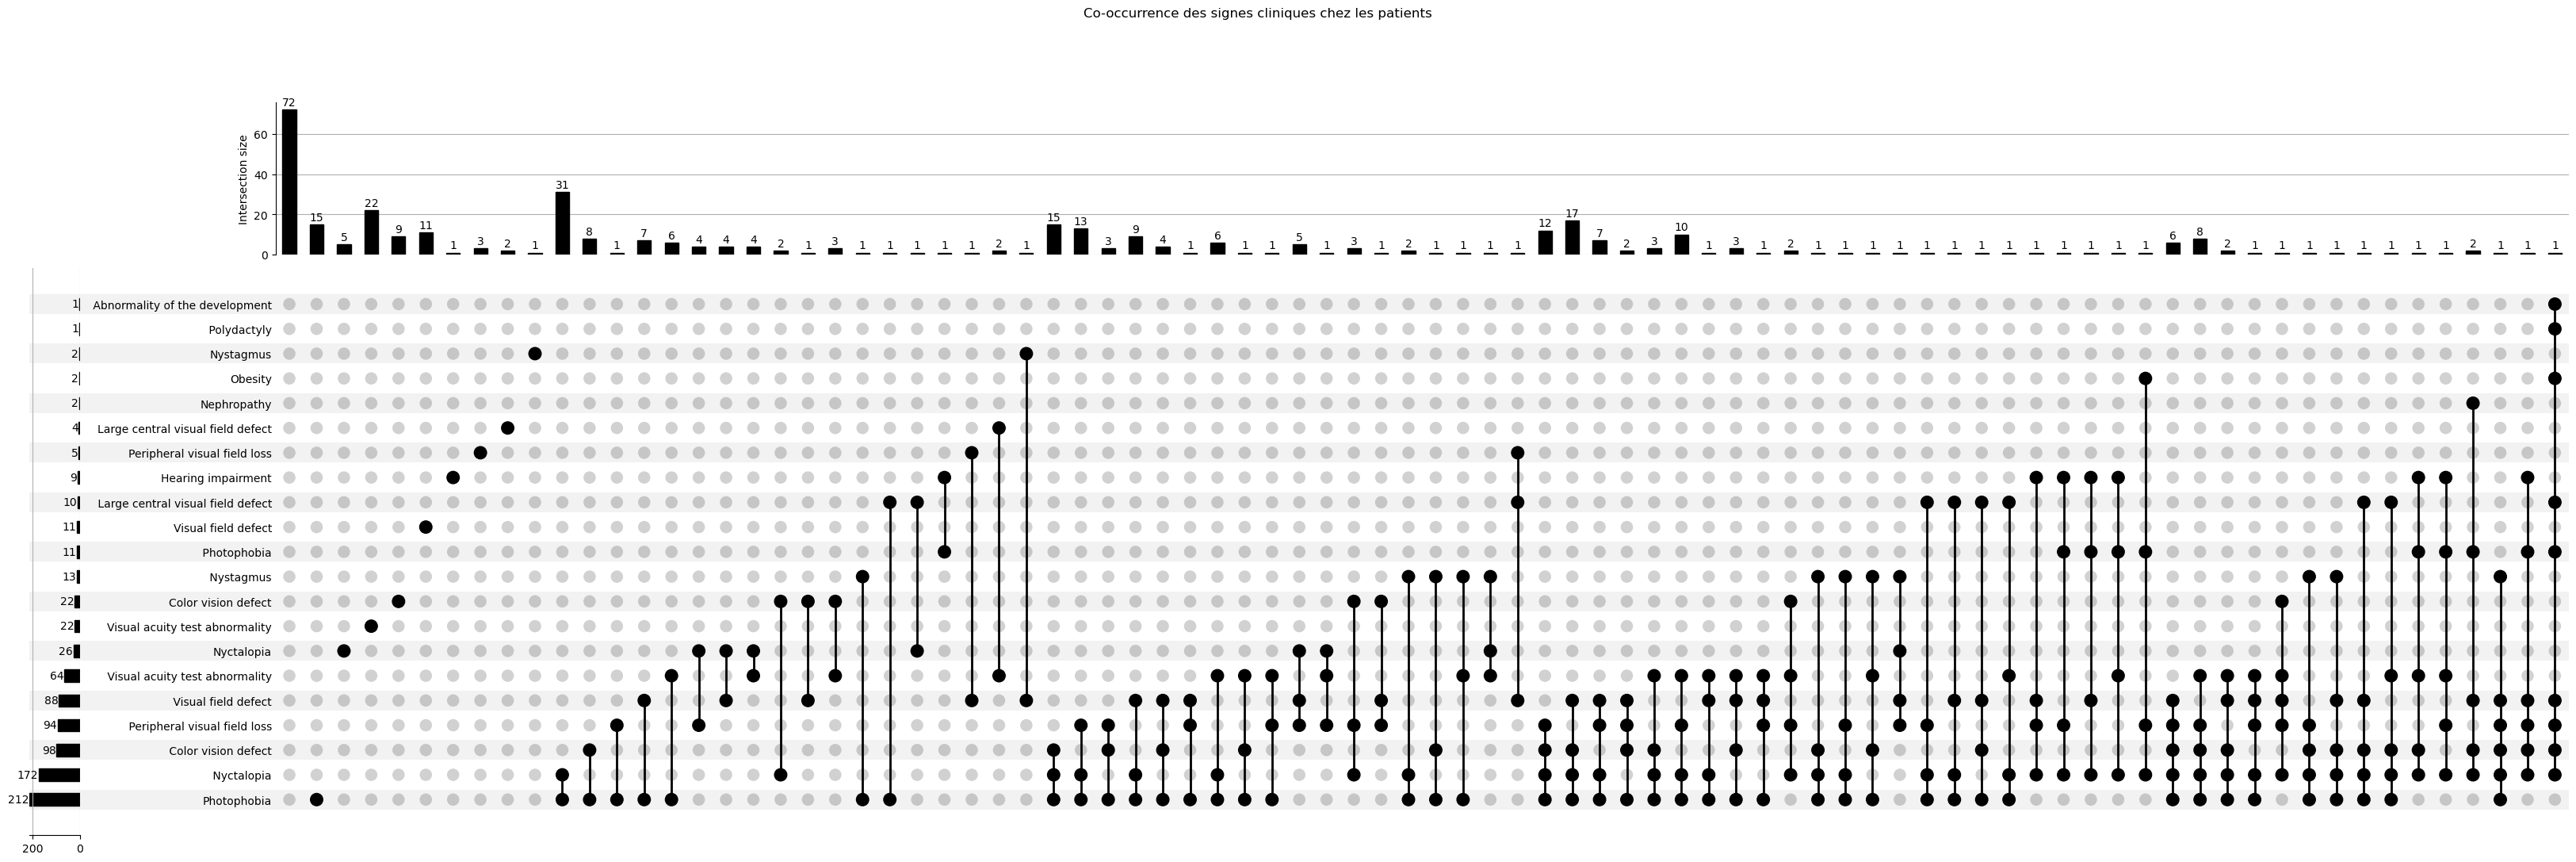
\includegraphics[keepaspectratio]{project_Fredd_files/figure-pdf/cell-22-output-2.png}}

\paragraph{2.5.5 Investigations réalisées sur le
patient}\label{investigations-ruxe9alisuxe9es-sur-le-patient}

\begin{Shaded}
\begin{Highlighting}[]
\ImportTok{from}\NormalTok{ plotly.subplots }\ImportTok{import}\NormalTok{ make\_subplots}
\ImportTok{import}\NormalTok{ plotly.graph\_objects }\ImportTok{as}\NormalTok{ go}

\NormalTok{variables }\OperatorTok{=}\NormalTok{ [            }
    \StringTok{\textquotesingle{}diaCli\_invesCli\textquotesingle{}}\NormalTok{, }\StringTok{\textquotesingle{}diaCli\_invesBio\textquotesingle{}}\NormalTok{, }\StringTok{\textquotesingle{}diaCli\_invesBiol\textquotesingle{}}\NormalTok{, }\StringTok{\textquotesingle{}diaCli\_invesIma\textquotesingle{}}\NormalTok{,}
    \StringTok{\textquotesingle{}diaCli\_invesExp\textquotesingle{}}\NormalTok{, }\StringTok{\textquotesingle{}diaCli\_invesAna\textquotesingle{}}\NormalTok{, }\StringTok{\textquotesingle{}diaCli\_invesGen\textquotesingle{}}\NormalTok{, }\StringTok{\textquotesingle{}diaCli\_invesERG\textquotesingle{}}\NormalTok{, }\StringTok{\textquotesingle{}diaCli\_invesAut\textquotesingle{}}
\NormalTok{]}

\NormalTok{fig }\OperatorTok{=}\NormalTok{ make\_subplots(}
\NormalTok{    rows}\OperatorTok{=}\DecValTok{3}\NormalTok{, cols}\OperatorTok{=}\DecValTok{3}\NormalTok{,}
\NormalTok{    subplot\_titles}\OperatorTok{=}\NormalTok{variables,}
\NormalTok{    specs}\OperatorTok{=}\NormalTok{[[\{}\StringTok{"type"}\NormalTok{: }\StringTok{"domain"}\NormalTok{\}]}\OperatorTok{*}\DecValTok{3}\NormalTok{]}\OperatorTok{*}\DecValTok{3}
\NormalTok{)}

\NormalTok{couleurs }\OperatorTok{=}\NormalTok{ \{}
    \StringTok{\textquotesingle{}1\textquotesingle{}}\NormalTok{: }\StringTok{\textquotesingle{}green\textquotesingle{}}\NormalTok{,}
    \StringTok{\textquotesingle{}2\textquotesingle{}}\NormalTok{: }\StringTok{\textquotesingle{}firebrick\textquotesingle{}}\NormalTok{,}
    \StringTok{\textquotesingle{}nan\textquotesingle{}}\NormalTok{: }\StringTok{\textquotesingle{}lightgrey\textquotesingle{}}\NormalTok{,}
    \StringTok{\textquotesingle{}Genetic test\textquotesingle{}}\NormalTok{ : }\StringTok{\textquotesingle{}royalblue\textquotesingle{}}\NormalTok{,}
    \StringTok{\textquotesingle{}test de performance\textquotesingle{}}\NormalTok{ : }\StringTok{\textquotesingle{}yellow\textquotesingle{}}\NormalTok{,}
\NormalTok{\}}

\ControlFlowTok{for}\NormalTok{ i, col }\KeywordTok{in} \BuiltInTok{enumerate}\NormalTok{(variables):}
\NormalTok{    counts }\OperatorTok{=}\NormalTok{ data1[col].value\_counts(dropna}\OperatorTok{=}\VariableTok{False}\NormalTok{).reset\_index()}
\NormalTok{    counts.columns }\OperatorTok{=}\NormalTok{ [}\StringTok{\textquotesingle{}category\textquotesingle{}}\NormalTok{, }\StringTok{\textquotesingle{}count\textquotesingle{}}\NormalTok{]}
\NormalTok{    totals\_counts }\OperatorTok{=}\NormalTok{ counts[}\StringTok{\textquotesingle{}count\textquotesingle{}}\NormalTok{].}\BuiltInTok{sum}\NormalTok{()}
\NormalTok{    counts[}\StringTok{\textquotesingle{}Percentage\textquotesingle{}}\NormalTok{] }\OperatorTok{=}\NormalTok{ (counts[}\StringTok{\textquotesingle{}count\textquotesingle{}}\NormalTok{] }\OperatorTok{/}\NormalTok{ totals\_counts }\OperatorTok{*} \DecValTok{100}\NormalTok{).}\BuiltInTok{round}\NormalTok{(}\DecValTok{1}\NormalTok{)}
\NormalTok{    counts[}\StringTok{\textquotesingle{}category\textquotesingle{}}\NormalTok{] }\OperatorTok{=}\NormalTok{ counts[}\StringTok{\textquotesingle{}category\textquotesingle{}}\NormalTok{].astype(}\BuiltInTok{str}\NormalTok{)}
\NormalTok{    counts[}\StringTok{\textquotesingle{}label\textquotesingle{}}\NormalTok{] }\OperatorTok{=}\NormalTok{ counts[}\StringTok{\textquotesingle{}category\textquotesingle{}}\NormalTok{].replace(\{}\StringTok{\textquotesingle{}1\textquotesingle{}}\NormalTok{: }\StringTok{\textquotesingle{}Oui\textquotesingle{}}\NormalTok{, }\StringTok{\textquotesingle{}2\textquotesingle{}}\NormalTok{: }\StringTok{\textquotesingle{}Non\textquotesingle{}}\NormalTok{, }\StringTok{\textquotesingle{}nan\textquotesingle{}}\NormalTok{: }\StringTok{\textquotesingle{}Inconnu\textquotesingle{}}\NormalTok{\})}


\NormalTok{    pie }\OperatorTok{=}\NormalTok{ go.Pie(}
\NormalTok{        labels}\OperatorTok{=}\NormalTok{counts[}\StringTok{\textquotesingle{}label\textquotesingle{}}\NormalTok{],}
\NormalTok{        values}\OperatorTok{=}\NormalTok{counts[}\StringTok{\textquotesingle{}count\textquotesingle{}}\NormalTok{],}
\NormalTok{        marker\_colors}\OperatorTok{=}\NormalTok{[couleurs.get(x, }\StringTok{\textquotesingle{}grey\textquotesingle{}}\NormalTok{) }\ControlFlowTok{for}\NormalTok{ x }\KeywordTok{in}\NormalTok{ counts[}\StringTok{\textquotesingle{}category\textquotesingle{}}\NormalTok{]],}
\NormalTok{        textinfo}\OperatorTok{=}\StringTok{\textquotesingle{}percent+label+value\textquotesingle{}}\NormalTok{,}
\NormalTok{        showlegend}\OperatorTok{=}\VariableTok{False}  
\NormalTok{    )}

\NormalTok{    row }\OperatorTok{=}\NormalTok{ i }\OperatorTok{//} \DecValTok{3} \OperatorTok{+} \DecValTok{1}
\NormalTok{    col\_idx }\OperatorTok{=}\NormalTok{ i }\OperatorTok{\%} \DecValTok{3} \OperatorTok{+} \DecValTok{1}
\NormalTok{    fig.add\_trace(pie, row}\OperatorTok{=}\NormalTok{row, col}\OperatorTok{=}\NormalTok{col\_idx)}

\NormalTok{fig.update\_layout(}
\NormalTok{    height}\OperatorTok{=}\DecValTok{700}\NormalTok{, width}\OperatorTok{=}\DecValTok{800}\NormalTok{,}
\NormalTok{    title\_text}\OperatorTok{=}\StringTok{"\textless{}b\textgreater{}Investigations réalisées"}
\NormalTok{)}
\NormalTok{fig.show()}
\end{Highlighting}
\end{Shaded}

\begin{verbatim}
Unable to display output for mime type(s): text/html
\end{verbatim}

\subsubsection{2.6 Informations du test
génétique}\label{informations-du-test-guxe9nuxe9tique}

\paragraph{2.6.1 Listes des techniques pour le test
génétique}\label{listes-des-techniques-pour-le-test-guxe9nuxe9tique}

\begin{Shaded}
\begin{Highlighting}[]
\NormalTok{data1[}\StringTok{\textquotesingle{}diaGen\_liste\_tec\textquotesingle{}}\NormalTok{].unique()}
\end{Highlighting}
\end{Shaded}

\begin{verbatim}
array([nan,  2.,  9.,  1.,  7.,  6.,  5.])
\end{verbatim}

\begin{Shaded}
\begin{Highlighting}[]
\NormalTok{counts }\OperatorTok{=}\NormalTok{ data1[}\StringTok{\textquotesingle{}diaGen\_liste\_tec\textquotesingle{}}\NormalTok{].value\_counts(dropna}\OperatorTok{=}\VariableTok{False}\NormalTok{).reset\_index()}
\NormalTok{counts.columns }\OperatorTok{=}\NormalTok{ [}\StringTok{\textquotesingle{}category\textquotesingle{}}\NormalTok{, }\StringTok{\textquotesingle{}count\textquotesingle{}}\NormalTok{]}
\NormalTok{totals\_counts }\OperatorTok{=}\NormalTok{ counts[}\StringTok{\textquotesingle{}count\textquotesingle{}}\NormalTok{].}\BuiltInTok{sum}\NormalTok{()}
\NormalTok{counts[}\StringTok{\textquotesingle{}Percentage\textquotesingle{}}\NormalTok{] }\OperatorTok{=}\NormalTok{ (counts[}\StringTok{\textquotesingle{}count\textquotesingle{}}\NormalTok{] }\OperatorTok{/}\NormalTok{ totals\_counts }\OperatorTok{*} \DecValTok{100}\NormalTok{).}\BuiltInTok{round}\NormalTok{(}\DecValTok{1}\NormalTok{)}

\NormalTok{counts[}\StringTok{\textquotesingle{}category\textquotesingle{}}\NormalTok{] }\OperatorTok{=}\NormalTok{ counts[}\StringTok{\textquotesingle{}category\textquotesingle{}}\NormalTok{].astype(}\BuiltInTok{str}\NormalTok{)}
\NormalTok{counts[}\StringTok{\textquotesingle{}label\textquotesingle{}}\NormalTok{] }\OperatorTok{=}\NormalTok{ counts[}\StringTok{\textquotesingle{}category\textquotesingle{}}\NormalTok{].replace(\{}\StringTok{\textquotesingle{}1.0\textquotesingle{}}\NormalTok{: }\StringTok{\textquotesingle{}Séquençage SANGER simple\textquotesingle{}}\NormalTok{, }
                                              \StringTok{\textquotesingle{}2.0\textquotesingle{}}\NormalTok{: }\StringTok{\textquotesingle{}Séquençage ciblé avec panel de 10{-}30 gènes\textquotesingle{}}\NormalTok{, }
                                              \StringTok{\textquotesingle{}5.0\textquotesingle{}}\NormalTok{: }\StringTok{\textquotesingle{}PCR Quantitative\textquotesingle{}}\NormalTok{, }
                                              \StringTok{\textquotesingle{}6.0\textquotesingle{}}\NormalTok{: }\StringTok{\textquotesingle{}Séquençage exome entier (WES)\textquotesingle{}}\NormalTok{,}
                                              \StringTok{\textquotesingle{}7.0\textquotesingle{}}\NormalTok{: }\StringTok{\textquotesingle{}Séquençage génome entier (WGS)\textquotesingle{}}\NormalTok{, }
                                              \StringTok{\textquotesingle{}9.0\textquotesingle{}}\NormalTok{: }\StringTok{\textquotesingle{}Others\textquotesingle{}}\NormalTok{,}
                                              \StringTok{\textquotesingle{}nan\textquotesingle{}}\NormalTok{: }\StringTok{\textquotesingle{}Unknown\textquotesingle{}}\NormalTok{\})}


\NormalTok{fig }\OperatorTok{=}\NormalTok{ px.pie(}
\NormalTok{        counts,}
\NormalTok{        names}\OperatorTok{=}\StringTok{\textquotesingle{}label\textquotesingle{}}\NormalTok{,}
\NormalTok{        values}\OperatorTok{=}\StringTok{\textquotesingle{}count\textquotesingle{}}\NormalTok{,}
\NormalTok{        title}\OperatorTok{=}\SpecialStringTok{f"\textless{}b\textgreater{}Methodes utilisées pour le test génétique"}\NormalTok{,}
\NormalTok{        color\_discrete\_sequence}\OperatorTok{=}\NormalTok{px.colors.qualitative.Bold}

\NormalTok{    )}
\NormalTok{fig.update\_traces(textposition}\OperatorTok{=}\StringTok{\textquotesingle{}inside\textquotesingle{}}\NormalTok{, textinfo}\OperatorTok{=}\StringTok{\textquotesingle{}percent+label+value\textquotesingle{}}\NormalTok{)}
\NormalTok{fig.update\_layout(}
\NormalTok{    width}\OperatorTok{=}\DecValTok{850}\NormalTok{,  }
\NormalTok{    height}\OperatorTok{=}\DecValTok{450}\NormalTok{,  }
\NormalTok{    margin}\OperatorTok{=}\BuiltInTok{dict}\NormalTok{(t}\OperatorTok{=}\DecValTok{50}\NormalTok{, b}\OperatorTok{=}\DecValTok{50}\NormalTok{, l}\OperatorTok{=}\DecValTok{50}\NormalTok{, r}\OperatorTok{=}\DecValTok{50}\NormalTok{)}
\NormalTok{)}
\NormalTok{fig.show()}
\end{Highlighting}
\end{Shaded}

\begin{verbatim}
Unable to display output for mime type(s): text/html
\end{verbatim}

\paragraph{2.6.2 Statut du dernier test
génétique}\label{statut-du-dernier-test-guxe9nuxe9tique}

\begin{Shaded}
\begin{Highlighting}[]
\NormalTok{counts }\OperatorTok{=}\NormalTok{ data1[}\StringTok{\textquotesingle{}diaGen\_statut\_analyse\textquotesingle{}}\NormalTok{].value\_counts(dropna}\OperatorTok{=}\VariableTok{False}\NormalTok{).reset\_index()}
\NormalTok{counts.columns }\OperatorTok{=}\NormalTok{ [}\StringTok{\textquotesingle{}category\textquotesingle{}}\NormalTok{, }\StringTok{\textquotesingle{}count\textquotesingle{}}\NormalTok{]}
\NormalTok{totals\_counts }\OperatorTok{=}\NormalTok{ counts[}\StringTok{\textquotesingle{}count\textquotesingle{}}\NormalTok{].}\BuiltInTok{sum}\NormalTok{()}
\NormalTok{counts[}\StringTok{\textquotesingle{}Percentage\textquotesingle{}}\NormalTok{] }\OperatorTok{=}\NormalTok{ (counts[}\StringTok{\textquotesingle{}count\textquotesingle{}}\NormalTok{] }\OperatorTok{/}\NormalTok{ totals\_counts }\OperatorTok{*} \DecValTok{100}\NormalTok{).}\BuiltInTok{round}\NormalTok{(}\DecValTok{1}\NormalTok{)}

\NormalTok{counts[}\StringTok{\textquotesingle{}category\textquotesingle{}}\NormalTok{] }\OperatorTok{=}\NormalTok{ counts[}\StringTok{\textquotesingle{}category\textquotesingle{}}\NormalTok{].astype(}\BuiltInTok{str}\NormalTok{)}
\NormalTok{counts[}\StringTok{\textquotesingle{}label\textquotesingle{}}\NormalTok{] }\OperatorTok{=}\NormalTok{ counts[}\StringTok{\textquotesingle{}category\textquotesingle{}}\NormalTok{].replace(\{}\StringTok{\textquotesingle{}1\textquotesingle{}}\NormalTok{: }\StringTok{\textquotesingle{}En cours\textquotesingle{}}\NormalTok{, }
                                              \StringTok{\textquotesingle{}2\textquotesingle{}}\NormalTok{: }\StringTok{\textquotesingle{}Terminé\textquotesingle{}}\NormalTok{,}
                                              \StringTok{\textquotesingle{}3\textquotesingle{}}\NormalTok{: }\StringTok{\textquotesingle{}Inconnu\textquotesingle{}}
\NormalTok{                                             \})}


\NormalTok{fig }\OperatorTok{=}\NormalTok{ px.pie(}
\NormalTok{        counts,}
\NormalTok{        names}\OperatorTok{=}\StringTok{\textquotesingle{}label\textquotesingle{}}\NormalTok{,}
\NormalTok{        values}\OperatorTok{=}\StringTok{\textquotesingle{}count\textquotesingle{}}\NormalTok{,}
\NormalTok{        title}\OperatorTok{=}\SpecialStringTok{f"\textless{}b\textgreater{}Statut du dernier test génétique\textless{}b\textgreater{}"}\NormalTok{,}
\NormalTok{        color\_discrete\_sequence}\OperatorTok{=}\NormalTok{px.colors.qualitative.Bold}

\NormalTok{    )}
\NormalTok{fig.update\_traces(textposition}\OperatorTok{=}\StringTok{\textquotesingle{}inside\textquotesingle{}}\NormalTok{, textinfo}\OperatorTok{=}\StringTok{\textquotesingle{}percent+label+value\textquotesingle{}}\NormalTok{)}
\NormalTok{fig.update\_layout(}
\NormalTok{    width}\OperatorTok{=}\DecValTok{850}\NormalTok{,  }
\NormalTok{    height}\OperatorTok{=}\DecValTok{450}\NormalTok{,  }
\NormalTok{    margin}\OperatorTok{=}\BuiltInTok{dict}\NormalTok{(t}\OperatorTok{=}\DecValTok{50}\NormalTok{, b}\OperatorTok{=}\DecValTok{50}\NormalTok{, l}\OperatorTok{=}\DecValTok{50}\NormalTok{, r}\OperatorTok{=}\DecValTok{50}\NormalTok{)}
\NormalTok{)}
\NormalTok{fig.show()}
\end{Highlighting}
\end{Shaded}

\begin{verbatim}
Unable to display output for mime type(s): text/html
\end{verbatim}

\paragraph{2.6.3 Analyse des patients n'ayant pas de date du test
génétique}\label{analyse-des-patients-nayant-pas-de-date-du-test-guxe9nuxe9tique}

\begin{Shaded}
\begin{Highlighting}[]
\BuiltInTok{print}\NormalTok{(data1[}\StringTok{\textquotesingle{}diaGen\_CR\_date\textquotesingle{}}\NormalTok{].value\_counts().}\BuiltInTok{sum}\NormalTok{(), }\StringTok{"dates présentes"}\NormalTok{)}
\end{Highlighting}
\end{Shaded}

\begin{verbatim}
190 dates présentes
\end{verbatim}

\begin{Shaded}
\begin{Highlighting}[]
\NormalTok{data1[(data1[}\StringTok{\textquotesingle{}diaGen\_CR\_date\textquotesingle{}}\NormalTok{].isna()) }\OperatorTok{\&}\NormalTok{ (data1[}\StringTok{\textquotesingle{}diaGen\_statut\_analyse\textquotesingle{}}\NormalTok{] }\OperatorTok{==} \DecValTok{2}\NormalTok{)][}
\NormalTok{[}\StringTok{\textquotesingle{}adm\_date\_naissance\textquotesingle{}}\NormalTok{, }\StringTok{\textquotesingle{}diaGen\_statut\_analyse\textquotesingle{}}\NormalTok{, }\StringTok{\textquotesingle{}diaGen\_CR\_date\textquotesingle{}}\NormalTok{,}\StringTok{\textquotesingle{}diaGen\_caract\textquotesingle{}}\NormalTok{, }\StringTok{\textquotesingle{}diaGen\_var\_hgcn\_1\textquotesingle{}}\NormalTok{]].head(}\DecValTok{10}\NormalTok{)}
\end{Highlighting}
\end{Shaded}

\begin{longtable}[]{@{}llllll@{}}
\toprule\noalign{}
& adm\_date\_naissance & diaGen\_statut\_analyse & diaGen\_CR\_date &
diaGen\_caract & diaGen\_var\_hgcn\_1 \\
\midrule\noalign{}
\endhead
\bottomrule\noalign{}
\endlastfoot
0 & 1963-04-16 & 2 & NaT & True & WDR19 \\
2 & 2014-09-26 & 2 & NaT & True & CNGB3 \\
5 & 1969-12-12 & 2 & NaT & True & USH2A \\
6 & 1992-01-22 & 2 & NaT & True & CLRN1 \\
7 & 1951-07-09 & 2 & NaT & False & HGSNAT \\
9 & 2003-07-09 & 2 & NaT & False & CNGB1 \\
10 & 1954-10-13 & 2 & NaT & True & PRPH2 \\
20 & 1964-02-02 & 2 & NaT & True & PRPH2 \\
21 & 1946-07-07 & 2 & NaT & False & CNGA3 \\
23 & 2011-01-26 & 2 & NaT & True & ABCA4 \\
\end{longtable}

\paragraph{2.6.4 Patients n'ayant pas de Caractérisation du dernier test
génétique}\label{patients-nayant-pas-de-caractuxe9risation-du-dernier-test-guxe9nuxe9tique}

\begin{Shaded}
\begin{Highlighting}[]
\NormalTok{data\_car }\OperatorTok{=}\NormalTok{ data1[(data1[}\StringTok{\textquotesingle{}diaGen\_caract\textquotesingle{}}\NormalTok{].isna()) }\OperatorTok{\&}\NormalTok{ (data1[}\StringTok{\textquotesingle{}diaGen\_statut\_analyse\textquotesingle{}}\NormalTok{] }\OperatorTok{==} \DecValTok{2}\NormalTok{)][}
\NormalTok{[}\StringTok{\textquotesingle{}adm\_date\_naissance\textquotesingle{}}\NormalTok{, }\StringTok{\textquotesingle{}diaGen\_statut\_analyse\textquotesingle{}}\NormalTok{, }\StringTok{\textquotesingle{}diaGen\_caract\textquotesingle{}}\NormalTok{, }\StringTok{\textquotesingle{}diaGen\_var\_hgcn\_1\textquotesingle{}}\NormalTok{]]}
\NormalTok{data\_car}
\end{Highlighting}
\end{Shaded}

\begin{longtable}[]{@{}lllll@{}}
\toprule\noalign{}
& adm\_date\_naissance & diaGen\_statut\_analyse & diaGen\_caract &
diaGen\_var\_hgcn\_1 \\
\midrule\noalign{}
\endhead
\bottomrule\noalign{}
\endlastfoot
121 & 1982-04-29 & 2 & NaN & ATXN7 \\
273 & 1962-01-24 & 2 & NaN & CDK5RAP3 \\
\end{longtable}

\begin{Shaded}
\begin{Highlighting}[]
\NormalTok{counts }\OperatorTok{=}\NormalTok{ data1[}\StringTok{\textquotesingle{}diaGen\_caract\textquotesingle{}}\NormalTok{].value\_counts(dropna}\OperatorTok{=}\VariableTok{False}\NormalTok{).reset\_index()}
\NormalTok{counts.columns }\OperatorTok{=}\NormalTok{ [}\StringTok{\textquotesingle{}category\textquotesingle{}}\NormalTok{, }\StringTok{\textquotesingle{}count\textquotesingle{}}\NormalTok{]}
\NormalTok{totals\_counts }\OperatorTok{=}\NormalTok{ counts[}\StringTok{\textquotesingle{}count\textquotesingle{}}\NormalTok{].}\BuiltInTok{sum}\NormalTok{()}
\NormalTok{counts[}\StringTok{\textquotesingle{}Percentage\textquotesingle{}}\NormalTok{] }\OperatorTok{=}\NormalTok{ (counts[}\StringTok{\textquotesingle{}count\textquotesingle{}}\NormalTok{] }\OperatorTok{/}\NormalTok{ totals\_counts }\OperatorTok{*} \DecValTok{100}\NormalTok{).}\BuiltInTok{round}\NormalTok{(}\DecValTok{1}\NormalTok{)}

\NormalTok{counts[}\StringTok{\textquotesingle{}category\textquotesingle{}}\NormalTok{] }\OperatorTok{=}\NormalTok{ counts[}\StringTok{\textquotesingle{}category\textquotesingle{}}\NormalTok{].astype(}\BuiltInTok{str}\NormalTok{)}

\NormalTok{fig }\OperatorTok{=}\NormalTok{ px.pie(}
\NormalTok{        counts,}
\NormalTok{        names}\OperatorTok{=}\StringTok{\textquotesingle{}category\textquotesingle{}}\NormalTok{,}
\NormalTok{        values}\OperatorTok{=}\StringTok{\textquotesingle{}count\textquotesingle{}}\NormalTok{,}
\NormalTok{        title}\OperatorTok{=}\SpecialStringTok{f"\textless{}b\textgreater{}Caractérisation du dernier test génétique\textless{}b\textgreater{}"}\NormalTok{,}
\NormalTok{        color\_discrete\_sequence}\OperatorTok{=}\NormalTok{px.colors.qualitative.Bold}

\NormalTok{    )}
\NormalTok{fig.update\_traces(textposition}\OperatorTok{=}\StringTok{\textquotesingle{}inside\textquotesingle{}}\NormalTok{, textinfo}\OperatorTok{=}\StringTok{\textquotesingle{}percent+label+value\textquotesingle{}}\NormalTok{)}
\NormalTok{fig.update\_layout(}
\NormalTok{    width}\OperatorTok{=}\DecValTok{850}\NormalTok{,  }
\NormalTok{    height}\OperatorTok{=}\DecValTok{450}\NormalTok{,  }
\NormalTok{    margin}\OperatorTok{=}\BuiltInTok{dict}\NormalTok{(t}\OperatorTok{=}\DecValTok{50}\NormalTok{, b}\OperatorTok{=}\DecValTok{50}\NormalTok{, l}\OperatorTok{=}\DecValTok{50}\NormalTok{, r}\OperatorTok{=}\DecValTok{50}\NormalTok{)}
\NormalTok{)}
\NormalTok{fig.show()}
\end{Highlighting}
\end{Shaded}

\begin{verbatim}
Unable to display output for mime type(s): text/html
\end{verbatim}

\begin{Shaded}
\begin{Highlighting}[]
\NormalTok{data1[}\StringTok{"diaGen\_caract"}\NormalTok{].value\_counts()}
\end{Highlighting}
\end{Shaded}

\begin{verbatim}
diaGen_caract
True     297
False     50
Name: count, dtype: int64
\end{verbatim}

\subparagraph{Pas cohérent avec le statut du dernier
test}\label{pas-cohuxe9rent-avec-le-statut-du-dernier-test}

\paragraph{2.6.5 Nombre de Gène porteur par
patient}\label{nombre-de-guxe8ne-porteur-par-patient}

\begin{Shaded}
\begin{Highlighting}[]
\NormalTok{data1[}\StringTok{"diaGen\_var\_nbgene"}\NormalTok{].value\_counts()}
\end{Highlighting}
\end{Shaded}

\begin{verbatim}
diaGen_var_nbgene
1    319
0     65
2      5
Name: count, dtype: int64
\end{verbatim}

\begin{Shaded}
\begin{Highlighting}[]
\NormalTok{counts }\OperatorTok{=}\NormalTok{ data1[}\StringTok{\textquotesingle{}diaGen\_var\_nbgene\textquotesingle{}}\NormalTok{].value\_counts(dropna}\OperatorTok{=}\VariableTok{False}\NormalTok{).reset\_index()}
\NormalTok{counts.columns }\OperatorTok{=}\NormalTok{ [}\StringTok{\textquotesingle{}category\textquotesingle{}}\NormalTok{, }\StringTok{\textquotesingle{}count\textquotesingle{}}\NormalTok{]}
\NormalTok{totals\_counts }\OperatorTok{=}\NormalTok{ counts[}\StringTok{\textquotesingle{}count\textquotesingle{}}\NormalTok{].}\BuiltInTok{sum}\NormalTok{()}
\NormalTok{counts[}\StringTok{\textquotesingle{}Percentage\textquotesingle{}}\NormalTok{] }\OperatorTok{=}\NormalTok{ (counts[}\StringTok{\textquotesingle{}count\textquotesingle{}}\NormalTok{] }\OperatorTok{/}\NormalTok{ totals\_counts }\OperatorTok{*} \DecValTok{100}\NormalTok{).}\BuiltInTok{round}\NormalTok{(}\DecValTok{1}\NormalTok{)}

\NormalTok{counts[}\StringTok{\textquotesingle{}category\textquotesingle{}}\NormalTok{] }\OperatorTok{=}\NormalTok{ counts[}\StringTok{\textquotesingle{}category\textquotesingle{}}\NormalTok{].astype(}\BuiltInTok{str}\NormalTok{)}
\NormalTok{counts[}\StringTok{\textquotesingle{}label\textquotesingle{}}\NormalTok{] }\OperatorTok{=}\NormalTok{ counts[}\StringTok{\textquotesingle{}category\textquotesingle{}}\NormalTok{].replace(\{}\StringTok{\textquotesingle{}0\textquotesingle{}}\NormalTok{ : }\StringTok{\textquotesingle{}0 gene\textquotesingle{}}\NormalTok{, }\StringTok{\textquotesingle{}1\textquotesingle{}}\NormalTok{ : }\StringTok{\textquotesingle{}1 gene\textquotesingle{}}\NormalTok{, }\StringTok{\textquotesingle{}2\textquotesingle{}}\NormalTok{ : }\StringTok{\textquotesingle{}2 gene\textquotesingle{}}\NormalTok{\})}

\NormalTok{fig }\OperatorTok{=}\NormalTok{ px.pie(}
\NormalTok{        counts,}
\NormalTok{        names}\OperatorTok{=}\StringTok{\textquotesingle{}label\textquotesingle{}}\NormalTok{,}
\NormalTok{        values}\OperatorTok{=}\StringTok{\textquotesingle{}count\textquotesingle{}}\NormalTok{,}
\NormalTok{        title}\OperatorTok{=}\SpecialStringTok{f"\textless{}b\textgreater{}Nombre de patient porteur de 0, 1, 2 génes"}\NormalTok{,}
\NormalTok{        color\_discrete\_sequence}\OperatorTok{=}\NormalTok{px.colors.qualitative.Bold}

\NormalTok{    )}
\NormalTok{fig.update\_traces(textposition}\OperatorTok{=}\StringTok{\textquotesingle{}auto\textquotesingle{}}\NormalTok{, textinfo}\OperatorTok{=}\StringTok{\textquotesingle{}percent+label+value\textquotesingle{}}\NormalTok{)}
\NormalTok{fig.update\_layout(}
\NormalTok{    width}\OperatorTok{=}\DecValTok{850}\NormalTok{,  }
\NormalTok{    height}\OperatorTok{=}\DecValTok{450}\NormalTok{,  }
\NormalTok{    margin}\OperatorTok{=}\BuiltInTok{dict}\NormalTok{(t}\OperatorTok{=}\DecValTok{50}\NormalTok{, b}\OperatorTok{=}\DecValTok{50}\NormalTok{, l}\OperatorTok{=}\DecValTok{50}\NormalTok{, r}\OperatorTok{=}\DecValTok{50}\NormalTok{)}
\NormalTok{)}
\NormalTok{fig.show()}
\end{Highlighting}
\end{Shaded}

\begin{verbatim}
Unable to display output for mime type(s): text/html
\end{verbatim}

\paragraph{2.6.6 Patients ayant 2
gènes}\label{patients-ayant-2-guxe8nes}

\begin{Shaded}
\begin{Highlighting}[]
\NormalTok{data1[data1[}\StringTok{"diaGen\_var\_nbgene"}\NormalTok{] }\OperatorTok{==} \DecValTok{2}\NormalTok{][[}\StringTok{"adm\_date\_naissance"}\NormalTok{, }\StringTok{"diaGen\_var\_hgcn\_1"}\NormalTok{, }\StringTok{"diaGen\_var\_hgcn\_2"}\NormalTok{]]}
\end{Highlighting}
\end{Shaded}

\begin{longtable}[]{@{}llll@{}}
\toprule\noalign{}
& adm\_date\_naissance & diaGen\_var\_hgcn\_1 & diaGen\_var\_hgcn\_2 \\
\midrule\noalign{}
\endhead
\bottomrule\noalign{}
\endlastfoot
7 & 1951-07-09 & HGSNAT & PRPF31 \\
121 & 1982-04-29 & ATXN7 & SCAT7 \\
132 & 1971-04-10 & CLN3 & CRB1 \\
149 & 1992-05-08 & RPGR & RGR \\
363 & 1988-01-25 & CDHR1 & CDH23 \\
\end{longtable}

\paragraph{2.6.7 Listes des Gènes
repertoriés}\label{listes-des-guxe8nes-repertoriuxe9s}

\begin{Shaded}
\begin{Highlighting}[]
\ImportTok{import}\NormalTok{ plotly.express }\ImportTok{as}\NormalTok{ px}
\ImportTok{import}\NormalTok{ pandas }\ImportTok{as}\NormalTok{ pd}

\NormalTok{diagnosis\_counts }\OperatorTok{=}\NormalTok{ data1[}\StringTok{\textquotesingle{}diaGen\_var\_hgcn\_1\textquotesingle{}}\NormalTok{].value\_counts(dropna}\OperatorTok{=}\VariableTok{False}\NormalTok{).reset\_index()}
\NormalTok{diagnosis\_counts.columns }\OperatorTok{=}\NormalTok{ [}\StringTok{\textquotesingle{}Diagnosis\textquotesingle{}}\NormalTok{, }\StringTok{\textquotesingle{}Number of cases\textquotesingle{}}\NormalTok{]}

\NormalTok{diagnosis\_counts[}\StringTok{\textquotesingle{}Diagnosis\textquotesingle{}}\NormalTok{] }\OperatorTok{=}\NormalTok{ diagnosis\_counts[}\StringTok{\textquotesingle{}Diagnosis\textquotesingle{}}\NormalTok{].fillna(}\StringTok{\textquotesingle{}Missing\textquotesingle{}}\NormalTok{)}


\NormalTok{total\_cases }\OperatorTok{=}\NormalTok{ diagnosis\_counts[}\StringTok{\textquotesingle{}Number of cases\textquotesingle{}}\NormalTok{].}\BuiltInTok{sum}\NormalTok{()}
\NormalTok{diagnosis\_counts[}\StringTok{\textquotesingle{}Percentage\textquotesingle{}}\NormalTok{] }\OperatorTok{=}\NormalTok{ (diagnosis\_counts[}\StringTok{\textquotesingle{}Number of cases\textquotesingle{}}\NormalTok{] }\OperatorTok{/}\NormalTok{ total\_cases }\OperatorTok{*} \DecValTok{100}\NormalTok{).}\BuiltInTok{round}\NormalTok{(}\DecValTok{1}\NormalTok{)}

\NormalTok{fig }\OperatorTok{=}\NormalTok{ px.bar(}
\NormalTok{    diagnosis\_counts,}
\NormalTok{    y}\OperatorTok{=}\StringTok{\textquotesingle{}Diagnosis\textquotesingle{}}\NormalTok{,}
\NormalTok{    x}\OperatorTok{=}\StringTok{\textquotesingle{}Number of cases\textquotesingle{}}\NormalTok{,}
\NormalTok{    color}\OperatorTok{=}\StringTok{\textquotesingle{}Number of cases\textquotesingle{}}\NormalTok{,}
\NormalTok{    orientation}\OperatorTok{=}\StringTok{\textquotesingle{}h\textquotesingle{}}\NormalTok{,}
\NormalTok{    color\_continuous\_scale}\OperatorTok{=}\StringTok{\textquotesingle{}Plasma\textquotesingle{}}\NormalTok{,}
\NormalTok{    text}\OperatorTok{=}\StringTok{\textquotesingle{}Number of cases\textquotesingle{}}\NormalTok{,}
\NormalTok{    title}\OperatorTok{=}\StringTok{\textquotesingle{}\textless{}b\textgreater{}Répartition des gènes selon le test clinique\textless{}/b\textgreater{}\textquotesingle{}}\NormalTok{,}
\NormalTok{    labels}\OperatorTok{=}\NormalTok{\{}\StringTok{\textquotesingle{}Number of cases\textquotesingle{}}\NormalTok{: }\StringTok{\textquotesingle{}Nb cases\textquotesingle{}}\NormalTok{, }\StringTok{\textquotesingle{}Diagnosis\textquotesingle{}}\NormalTok{: }\StringTok{\textquotesingle{}Genes\textquotesingle{}}\NormalTok{\},}
\NormalTok{    height}\OperatorTok{=}\DecValTok{900}
\NormalTok{)}

\NormalTok{fig.update\_layout(}
\NormalTok{    yaxis}\OperatorTok{=}\NormalTok{\{}\StringTok{\textquotesingle{}categoryorder\textquotesingle{}}\NormalTok{:}\StringTok{\textquotesingle{}total ascending\textquotesingle{}}\NormalTok{\}, }
\NormalTok{    plot\_bgcolor}\OperatorTok{=}\StringTok{\textquotesingle{}rgba(0,0,0,0)\textquotesingle{}}\NormalTok{,}
\NormalTok{    hovermode}\OperatorTok{=}\StringTok{\textquotesingle{}y unified\textquotesingle{}}\NormalTok{,}
\NormalTok{    title\_font}\OperatorTok{=}\NormalTok{\{}\StringTok{\textquotesingle{}size\textquotesingle{}}\NormalTok{: }\DecValTok{20}\NormalTok{\},}
\NormalTok{    uniformtext\_minsize}\OperatorTok{=}\DecValTok{20}

\NormalTok{)}

\NormalTok{fig.update\_traces(}
\NormalTok{    texttemplate}\OperatorTok{=}\StringTok{\textquotesingle{}\textless{}b\textgreater{}\%}\SpecialCharTok{\{x\}}\StringTok{\textless{}/b\textgreater{}\textless{}br\textgreater{}(\%}\SpecialCharTok{\{customdata[0]\}}\StringTok{\%)\textquotesingle{}}\NormalTok{,}
\NormalTok{    hovertemplate}\OperatorTok{=}\StringTok{"\textless{}b\textgreater{}\%}\SpecialCharTok{\{y\}}\StringTok{\textless{}/b\textgreater{}\textless{}br\textgreater{}Cases: \%}\SpecialCharTok{\{x\}}\StringTok{\textless{}br\textgreater{}Proportion: \%}\SpecialCharTok{\{customdata[0]\}}\StringTok{\%"}\NormalTok{,}
\NormalTok{    textposition}\OperatorTok{=}\StringTok{\textquotesingle{}auto\textquotesingle{}}\NormalTok{,}
\NormalTok{    customdata}\OperatorTok{=}\NormalTok{diagnosis\_counts[[}\StringTok{\textquotesingle{}Percentage\textquotesingle{}}\NormalTok{]],}
\NormalTok{    textfont\_size}\OperatorTok{=}\DecValTok{30}\NormalTok{,}
\NormalTok{)}

\NormalTok{fig.show()}
\end{Highlighting}
\end{Shaded}

\begin{verbatim}
Unable to display output for mime type(s): text/html
\end{verbatim}

\paragraph{2.6.8 Méthodes de transmission de
gènes}\label{muxe9thodes-de-transmission-de-guxe8nes}

\begin{Shaded}
\begin{Highlighting}[]
\NormalTok{counts }\OperatorTok{=}\NormalTok{ data1[}\StringTok{\textquotesingle{}diaGen\_var\_trans\_1\textquotesingle{}}\NormalTok{].value\_counts(dropna}\OperatorTok{=}\VariableTok{False}\NormalTok{).reset\_index()}
\NormalTok{counts.columns }\OperatorTok{=}\NormalTok{ [}\StringTok{\textquotesingle{}category\textquotesingle{}}\NormalTok{, }\StringTok{\textquotesingle{}count\textquotesingle{}}\NormalTok{]}
\NormalTok{totals\_counts }\OperatorTok{=}\NormalTok{ counts[}\StringTok{\textquotesingle{}count\textquotesingle{}}\NormalTok{].}\BuiltInTok{sum}\NormalTok{()}
\NormalTok{counts[}\StringTok{\textquotesingle{}Percentage\textquotesingle{}}\NormalTok{] }\OperatorTok{=}\NormalTok{ (counts[}\StringTok{\textquotesingle{}count\textquotesingle{}}\NormalTok{] }\OperatorTok{/}\NormalTok{ totals\_counts }\OperatorTok{*} \DecValTok{100}\NormalTok{).}\BuiltInTok{round}\NormalTok{(}\DecValTok{1}\NormalTok{)}

\NormalTok{counts[}\StringTok{\textquotesingle{}category\textquotesingle{}}\NormalTok{] }\OperatorTok{=}\NormalTok{ counts[}\StringTok{\textquotesingle{}category\textquotesingle{}}\NormalTok{].astype(}\BuiltInTok{str}\NormalTok{)}
\NormalTok{counts[}\StringTok{\textquotesingle{}label\textquotesingle{}}\NormalTok{] }\OperatorTok{=}\NormalTok{ counts[}\StringTok{\textquotesingle{}category\textquotesingle{}}\NormalTok{].replace(\{}\StringTok{\textquotesingle{}1.0\textquotesingle{}}\NormalTok{: }\StringTok{\textquotesingle{}De novo\textquotesingle{}}\NormalTok{, }\StringTok{\textquotesingle{}2.0\textquotesingle{}}\NormalTok{: }\StringTok{\textquotesingle{}Autosomique dominant\textquotesingle{}}\NormalTok{, }
                                              \StringTok{\textquotesingle{}3.0\textquotesingle{}}\NormalTok{: }\StringTok{\textquotesingle{}Autosomique récessif\textquotesingle{}}\NormalTok{, }\StringTok{\textquotesingle{}nan\textquotesingle{}}\NormalTok{: }\StringTok{\textquotesingle{}Unknown\textquotesingle{}}\NormalTok{\})}


\NormalTok{fig }\OperatorTok{=}\NormalTok{ px.pie(}
\NormalTok{        counts,}
\NormalTok{        names}\OperatorTok{=}\StringTok{\textquotesingle{}label\textquotesingle{}}\NormalTok{,}
\NormalTok{        values}\OperatorTok{=}\StringTok{\textquotesingle{}count\textquotesingle{}}\NormalTok{,}
\NormalTok{        title}\OperatorTok{=}\SpecialStringTok{f"\textless{}b\textgreater{}Méthodes de transmission"}\NormalTok{,}
\NormalTok{        color\_discrete\_sequence}\OperatorTok{=}\NormalTok{px.colors.qualitative.Bold}

\NormalTok{    )}
\NormalTok{fig.update\_traces(textposition}\OperatorTok{=}\StringTok{\textquotesingle{}inside\textquotesingle{}}\NormalTok{, textinfo}\OperatorTok{=}\StringTok{\textquotesingle{}percent+label+value\textquotesingle{}}\NormalTok{)}
\NormalTok{fig.update\_layout(}
\NormalTok{    width}\OperatorTok{=}\DecValTok{850}\NormalTok{,  }
\NormalTok{    height}\OperatorTok{=}\DecValTok{450}\NormalTok{,  }
\NormalTok{    margin}\OperatorTok{=}\BuiltInTok{dict}\NormalTok{(t}\OperatorTok{=}\DecValTok{50}\NormalTok{, b}\OperatorTok{=}\DecValTok{50}\NormalTok{, l}\OperatorTok{=}\DecValTok{50}\NormalTok{, r}\OperatorTok{=}\DecValTok{50}\NormalTok{)}
\NormalTok{)}
\NormalTok{fig.show()}
\end{Highlighting}
\end{Shaded}

\begin{verbatim}
Unable to display output for mime type(s): text/html
\end{verbatim}

\subsubsection{2.7 Correlation genotype/
phenotype}\label{correlation-genotype-phenotype}

\begin{Shaded}
\begin{Highlighting}[]
\NormalTok{counts }\OperatorTok{=}\NormalTok{ data1[}\StringTok{\textquotesingle{}diaGen\_corr\textquotesingle{}}\NormalTok{].value\_counts(dropna}\OperatorTok{=}\VariableTok{False}\NormalTok{).reset\_index()}
\NormalTok{counts.columns }\OperatorTok{=}\NormalTok{ [}\StringTok{\textquotesingle{}category\textquotesingle{}}\NormalTok{, }\StringTok{\textquotesingle{}count\textquotesingle{}}\NormalTok{]}
\NormalTok{totals\_counts }\OperatorTok{=}\NormalTok{ counts[}\StringTok{\textquotesingle{}count\textquotesingle{}}\NormalTok{].}\BuiltInTok{sum}\NormalTok{()}
\NormalTok{counts[}\StringTok{\textquotesingle{}Percentage\textquotesingle{}}\NormalTok{] }\OperatorTok{=}\NormalTok{ (counts[}\StringTok{\textquotesingle{}count\textquotesingle{}}\NormalTok{] }\OperatorTok{/}\NormalTok{ totals\_counts }\OperatorTok{*} \DecValTok{100}\NormalTok{).}\BuiltInTok{round}\NormalTok{(}\DecValTok{1}\NormalTok{)}

\NormalTok{counts[}\StringTok{\textquotesingle{}category\textquotesingle{}}\NormalTok{] }\OperatorTok{=}\NormalTok{ counts[}\StringTok{\textquotesingle{}category\textquotesingle{}}\NormalTok{].astype(}\BuiltInTok{str}\NormalTok{)}
\NormalTok{counts[}\StringTok{\textquotesingle{}label\textquotesingle{}}\NormalTok{] }\OperatorTok{=}\NormalTok{ counts[}\StringTok{\textquotesingle{}category\textquotesingle{}}\NormalTok{].replace(\{}\StringTok{\textquotesingle{}1.0\textquotesingle{}}\NormalTok{: }\StringTok{\textquotesingle{}Yes(cas classique)\textquotesingle{}}\NormalTok{,  }
                                              \StringTok{\textquotesingle{}0.0\textquotesingle{}}\NormalTok{: }\StringTok{\textquotesingle{}No(cas atypique) \textquotesingle{}}\NormalTok{, }
                                              \StringTok{\textquotesingle{}nan\textquotesingle{}}\NormalTok{: }\StringTok{\textquotesingle{}Inconnu\textquotesingle{}}\NormalTok{\})}


\NormalTok{fig }\OperatorTok{=}\NormalTok{ px.pie(}
\NormalTok{        counts,}
\NormalTok{        names}\OperatorTok{=}\StringTok{\textquotesingle{}label\textquotesingle{}}\NormalTok{,}
\NormalTok{        values}\OperatorTok{=}\StringTok{\textquotesingle{}count\textquotesingle{}}\NormalTok{,}
\NormalTok{        title}\OperatorTok{=}\SpecialStringTok{f"\textless{}b\textgreater{}Correlation Genotype/Phenotype"}\NormalTok{,}
\NormalTok{        color\_discrete\_sequence}\OperatorTok{=}\NormalTok{px.colors.qualitative.Bold}

\NormalTok{    )}
\NormalTok{fig.update\_traces(textposition}\OperatorTok{=}\StringTok{\textquotesingle{}inside\textquotesingle{}}\NormalTok{, textinfo}\OperatorTok{=}\StringTok{\textquotesingle{}percent+label+value\textquotesingle{}}\NormalTok{)}
\NormalTok{fig.update\_layout(}
\NormalTok{    width}\OperatorTok{=}\DecValTok{850}\NormalTok{,  }
\NormalTok{    height}\OperatorTok{=}\DecValTok{450}\NormalTok{,  }
\NormalTok{    margin}\OperatorTok{=}\BuiltInTok{dict}\NormalTok{(t}\OperatorTok{=}\DecValTok{50}\NormalTok{, b}\OperatorTok{=}\DecValTok{50}\NormalTok{, l}\OperatorTok{=}\DecValTok{50}\NormalTok{, r}\OperatorTok{=}\DecValTok{50}\NormalTok{)}
\NormalTok{)}
\NormalTok{fig.show()}
\end{Highlighting}
\end{Shaded}

\begin{verbatim}
Unable to display output for mime type(s): text/html
\end{verbatim}

\begin{Shaded}
\begin{Highlighting}[]
\ImportTok{import}\NormalTok{ seaborn }\ImportTok{as}\NormalTok{ sns}
\ImportTok{import}\NormalTok{ matplotlib.pyplot }\ImportTok{as}\NormalTok{ plt}

\NormalTok{pivot }\OperatorTok{=}\NormalTok{ data1.pivot\_table(}
\NormalTok{    index}\OperatorTok{=}\StringTok{\textquotesingle{}diaCli\_diagMR\_nom\textquotesingle{}}\NormalTok{,}
\NormalTok{    columns}\OperatorTok{=}\StringTok{\textquotesingle{}diaGen\_var\_hgcn\_1\textquotesingle{}}\NormalTok{,}
\NormalTok{    aggfunc}\OperatorTok{=}\StringTok{\textquotesingle{}size\textquotesingle{}}\NormalTok{,}
\NormalTok{    fill\_value}\OperatorTok{=}\DecValTok{0}
\NormalTok{)}

\NormalTok{plt.figure(figsize}\OperatorTok{=}\NormalTok{(}\DecValTok{18}\NormalTok{, }\DecValTok{10}\NormalTok{))}
\NormalTok{sns.heatmap(pivot, cmap}\OperatorTok{=}\StringTok{\textquotesingle{}YlGnBu\textquotesingle{}}\NormalTok{, annot}\OperatorTok{=}\VariableTok{True}\NormalTok{, fmt}\OperatorTok{=}\StringTok{"d"}\NormalTok{)}
\NormalTok{plt.title(}\StringTok{"Fréquence des combinaisons Diagnostic {-} Gène"}\NormalTok{)}
\NormalTok{plt.ylabel(}\StringTok{"Diagnostic"}\NormalTok{)}
\NormalTok{plt.xlabel(}\StringTok{"Gène identifié"}\NormalTok{)}
\NormalTok{plt.tight\_layout()}
\NormalTok{plt.show()}
\end{Highlighting}
\end{Shaded}

\pandocbounded{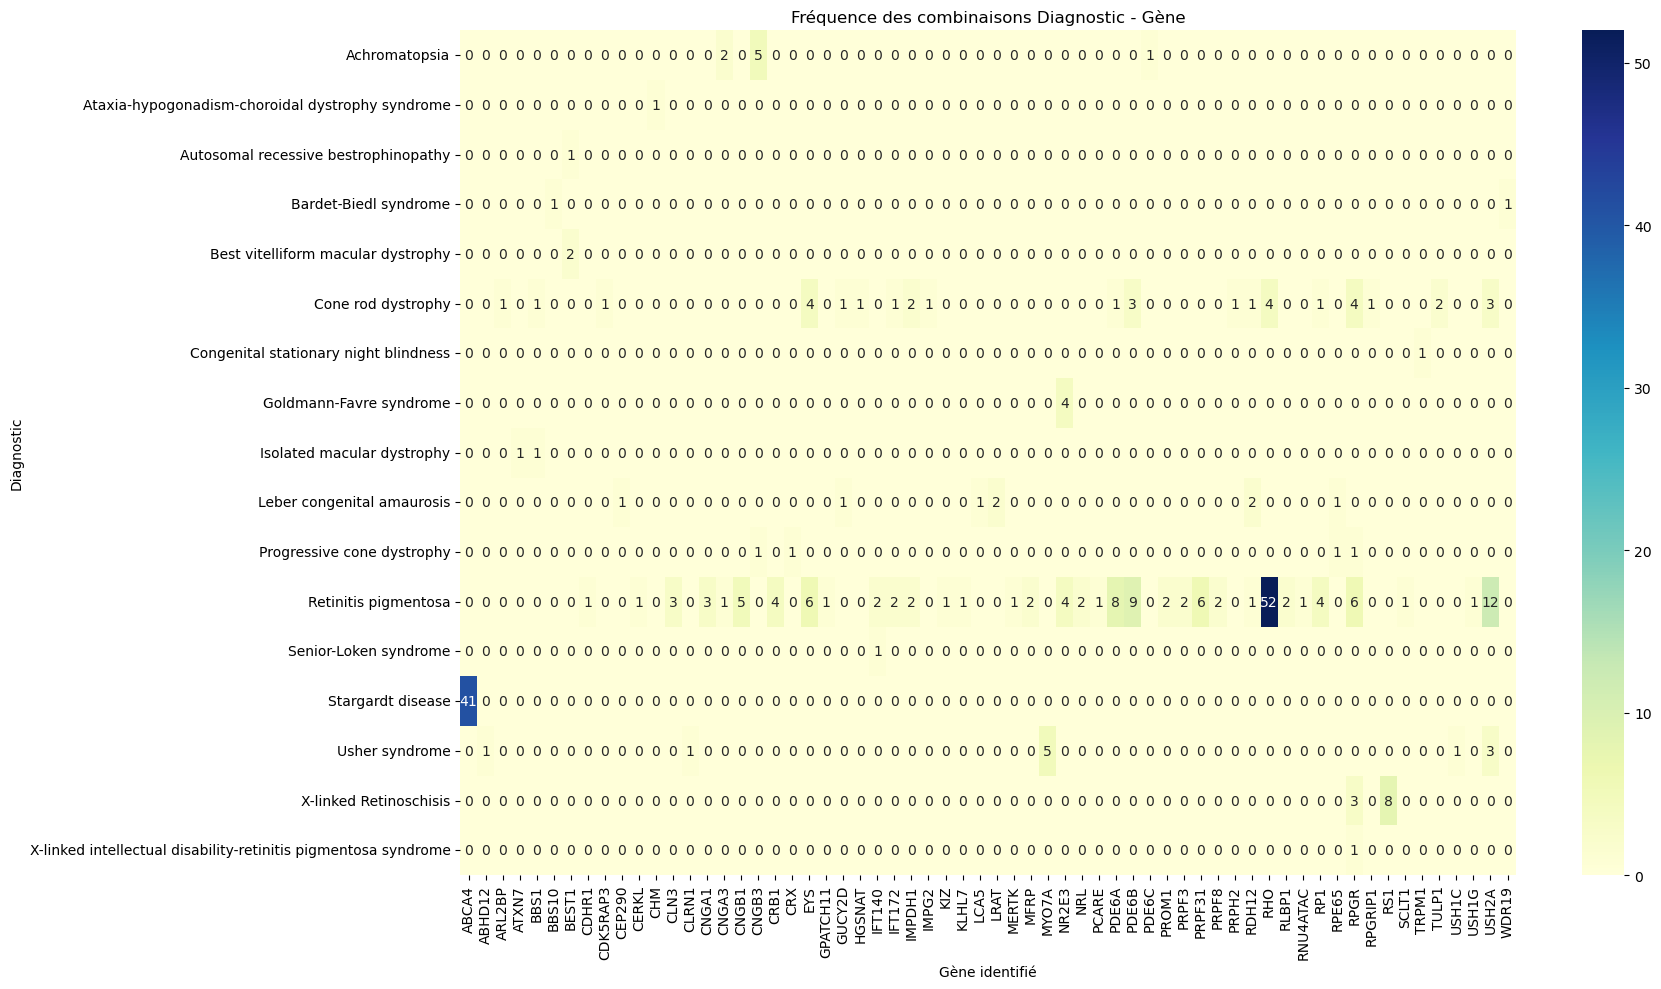
\includegraphics[keepaspectratio]{project_Fredd_files/figure-pdf/cell-38-output-1.png}}

\subsubsection{2.8 Examen Acuité
visuelle}\label{examen-acuituxe9-visuelle}

\begin{Shaded}
\begin{Highlighting}[]
\NormalTok{data1[}\StringTok{"exaAcu\_type\_examen\_OG"}\NormalTok{].unique()}
\end{Highlighting}
\end{Shaded}

\begin{verbatim}
array([ 5.,  6., nan,  1.])
\end{verbatim}

\begin{Shaded}
\begin{Highlighting}[]
\ImportTok{from}\NormalTok{ plotly.subplots }\ImportTok{import}\NormalTok{ make\_subplots}
\ImportTok{import}\NormalTok{ plotly.graph\_objects }\ImportTok{as}\NormalTok{ go}

\NormalTok{variables }\OperatorTok{=}\NormalTok{ [}\StringTok{\textquotesingle{}exaAcu\_type\_examen\_OG\textquotesingle{}}\NormalTok{, }\StringTok{\textquotesingle{}exaAcu\_type\_examen\_OD\textquotesingle{}}\NormalTok{]}

\NormalTok{fig }\OperatorTok{=}\NormalTok{ make\_subplots(}
\NormalTok{    rows}\OperatorTok{=}\DecValTok{1}\NormalTok{, cols}\OperatorTok{=}\DecValTok{2}\NormalTok{,}
\NormalTok{    subplot\_titles}\OperatorTok{=}\NormalTok{variables,}
\NormalTok{    specs}\OperatorTok{=}\NormalTok{[[\{}\StringTok{\textquotesingle{}type\textquotesingle{}}\NormalTok{: }\StringTok{\textquotesingle{}domain\textquotesingle{}}\NormalTok{\}, \{}\StringTok{\textquotesingle{}type\textquotesingle{}}\NormalTok{: }\StringTok{\textquotesingle{}domain\textquotesingle{}}\NormalTok{\}]]}
\NormalTok{)}

\ControlFlowTok{for}\NormalTok{ i, col }\KeywordTok{in} \BuiltInTok{enumerate}\NormalTok{(variables):}
\NormalTok{    counts }\OperatorTok{=}\NormalTok{ data1[col].value\_counts(dropna}\OperatorTok{=}\VariableTok{False}\NormalTok{).reset\_index()}
\NormalTok{    counts.columns }\OperatorTok{=}\NormalTok{ [}\StringTok{\textquotesingle{}category\textquotesingle{}}\NormalTok{, }\StringTok{\textquotesingle{}count\textquotesingle{}}\NormalTok{]}
\NormalTok{    totals\_counts }\OperatorTok{=}\NormalTok{ counts[}\StringTok{\textquotesingle{}count\textquotesingle{}}\NormalTok{].}\BuiltInTok{sum}\NormalTok{()}
\NormalTok{    counts[}\StringTok{\textquotesingle{}Percentage\textquotesingle{}}\NormalTok{] }\OperatorTok{=}\NormalTok{ (counts[}\StringTok{\textquotesingle{}count\textquotesingle{}}\NormalTok{] }\OperatorTok{/}\NormalTok{ totals\_counts }\OperatorTok{*} \DecValTok{100}\NormalTok{).}\BuiltInTok{round}\NormalTok{(}\DecValTok{1}\NormalTok{)}
\NormalTok{    counts[}\StringTok{\textquotesingle{}category\textquotesingle{}}\NormalTok{] }\OperatorTok{=}\NormalTok{ counts[}\StringTok{\textquotesingle{}category\textquotesingle{}}\NormalTok{].astype(}\BuiltInTok{str}\NormalTok{)}
\NormalTok{    counts[}\StringTok{\textquotesingle{}label\textquotesingle{}}\NormalTok{] }\OperatorTok{=}\NormalTok{ counts[}\StringTok{\textquotesingle{}category\textquotesingle{}}\NormalTok{].replace(\{}\StringTok{\textquotesingle{}1.0\textquotesingle{}}\NormalTok{: }\StringTok{\textquotesingle{}Monoyer\textquotesingle{}}\NormalTok{, }\StringTok{\textquotesingle{}2.0\textquotesingle{}}\NormalTok{: }\StringTok{\textquotesingle{}Pigassou\textquotesingle{}}\NormalTok{,}
                                                  \StringTok{\textquotesingle{}3.0\textquotesingle{}}\NormalTok{: }\StringTok{\textquotesingle{}Bébé vision\textquotesingle{}}\NormalTok{, }\StringTok{\textquotesingle{}4.0\textquotesingle{}}\NormalTok{: }\StringTok{\textquotesingle{}Cardiff\textquotesingle{}}\NormalTok{,}
                                                 \StringTok{\textquotesingle{}5.0\textquotesingle{}}\NormalTok{: }\StringTok{\textquotesingle{}EDTRS\textquotesingle{}}\NormalTok{,}\StringTok{\textquotesingle{}6.0\textquotesingle{}}\NormalTok{ : }\StringTok{\textquotesingle{}Autre\textquotesingle{}}\NormalTok{\})}
\NormalTok{    pie }\OperatorTok{=}\NormalTok{ go.Pie(}
\NormalTok{        labels}\OperatorTok{=}\NormalTok{counts[}\StringTok{\textquotesingle{}label\textquotesingle{}}\NormalTok{],}
\NormalTok{        values}\OperatorTok{=}\NormalTok{counts[}\StringTok{\textquotesingle{}count\textquotesingle{}}\NormalTok{],}
\NormalTok{        textinfo}\OperatorTok{=}\StringTok{\textquotesingle{}percent+label\textquotesingle{}}\NormalTok{,}
\NormalTok{        showlegend}\OperatorTok{=}\VariableTok{False}  
\NormalTok{    )}

\NormalTok{    row }\OperatorTok{=} \DecValTok{1}
\NormalTok{    col\_idx }\OperatorTok{=}\NormalTok{ i }\OperatorTok{+} \DecValTok{1}
\NormalTok{    fig.add\_trace(pie, row}\OperatorTok{=}\NormalTok{row, col}\OperatorTok{=}\NormalTok{col\_idx)}

\NormalTok{fig.update\_layout(}
\NormalTok{    height}\OperatorTok{=}\DecValTok{450}\NormalTok{, width}\OperatorTok{=}\DecValTok{850}\NormalTok{,}
\NormalTok{    title\_text}\OperatorTok{=}\StringTok{"\textless{}b\textgreater{}Types d\textquotesingle{}examen pour la mesure de l\textquotesingle{}acuité visuelle\textless{}/b\textgreater{}"}
\NormalTok{)}
\NormalTok{fig.update\_traces(textposition}\OperatorTok{=}\StringTok{\textquotesingle{}inside\textquotesingle{}}\NormalTok{, textinfo}\OperatorTok{=}\StringTok{\textquotesingle{}percent+label+value\textquotesingle{}}\NormalTok{)}

\NormalTok{fig.show()}
\end{Highlighting}
\end{Shaded}

\begin{verbatim}
Unable to display output for mime type(s): text/html
\end{verbatim}

\subsubsection{2.9 Examen champ visuel}\label{examen-champ-visuel}

\begin{Shaded}
\begin{Highlighting}[]
\NormalTok{data1[}\StringTok{\textquotesingle{}exaChv\_fait\textquotesingle{}}\NormalTok{].unique()}
\end{Highlighting}
\end{Shaded}

\begin{verbatim}
array([ True, False])
\end{verbatim}

\begin{Shaded}
\begin{Highlighting}[]
\NormalTok{proportions }\OperatorTok{=}\NormalTok{ data1[}\StringTok{\textquotesingle{}exaChv\_fait\textquotesingle{}}\NormalTok{].value\_counts().reset\_index()}
\NormalTok{proportions.columns }\OperatorTok{=}\NormalTok{ [}\StringTok{\textquotesingle{}exaChv\_fait\textquotesingle{}}\NormalTok{, }\StringTok{\textquotesingle{}proportion\textquotesingle{}}\NormalTok{]}
\NormalTok{totals\_counts }\OperatorTok{=}\NormalTok{ proportions[}\StringTok{\textquotesingle{}proportion\textquotesingle{}}\NormalTok{].}\BuiltInTok{sum}\NormalTok{()}
\NormalTok{proportions[}\StringTok{\textquotesingle{}Percentage\textquotesingle{}}\NormalTok{] }\OperatorTok{=}\NormalTok{ (proportions[}\StringTok{\textquotesingle{}proportion\textquotesingle{}}\NormalTok{] }\OperatorTok{/}\NormalTok{ totals\_counts }\OperatorTok{*} \DecValTok{100}\NormalTok{).}\BuiltInTok{round}\NormalTok{(}\DecValTok{1}\NormalTok{)}

\NormalTok{proportions[}\StringTok{\textquotesingle{}exaChv\_fait\textquotesingle{}}\NormalTok{] }\OperatorTok{=}\NormalTok{ proportions[}\StringTok{\textquotesingle{}exaChv\_fait\textquotesingle{}}\NormalTok{].astype(}\BuiltInTok{str}\NormalTok{)}
\NormalTok{proportions[}\StringTok{\textquotesingle{}label\textquotesingle{}}\NormalTok{] }\OperatorTok{=}\NormalTok{ proportions[}\StringTok{\textquotesingle{}exaChv\_fait\textquotesingle{}}\NormalTok{].replace(\{}\StringTok{\textquotesingle{}True\textquotesingle{}}\NormalTok{: }\StringTok{\textquotesingle{}Oui\textquotesingle{}}\NormalTok{, }\StringTok{\textquotesingle{}False\textquotesingle{}}\NormalTok{: }\StringTok{\textquotesingle{}Non\textquotesingle{}}\NormalTok{\})}

\NormalTok{fig }\OperatorTok{=}\NormalTok{ px.pie(}
\NormalTok{        proportions,}
\NormalTok{        names}\OperatorTok{=}\StringTok{\textquotesingle{}label\textquotesingle{}}\NormalTok{,}
\NormalTok{        values}\OperatorTok{=}\StringTok{\textquotesingle{}proportion\textquotesingle{}}\NormalTok{,}
\NormalTok{        title}\OperatorTok{=}\SpecialStringTok{f"\textless{}b\textgreater{} Examen champ visuel réalisé"}\NormalTok{,}
\NormalTok{        color\_discrete\_sequence}\OperatorTok{=}\NormalTok{px.colors.qualitative.Bold}

\NormalTok{    )}
\NormalTok{fig.update\_traces(textposition}\OperatorTok{=}\StringTok{\textquotesingle{}inside\textquotesingle{}}\NormalTok{, textinfo}\OperatorTok{=}\StringTok{\textquotesingle{}percent+label+value\textquotesingle{}}\NormalTok{)}
\NormalTok{fig.update\_layout(}
\NormalTok{    width}\OperatorTok{=}\DecValTok{850}\NormalTok{,  }
\NormalTok{    height}\OperatorTok{=}\DecValTok{450}\NormalTok{,  }
\NormalTok{    margin}\OperatorTok{=}\BuiltInTok{dict}\NormalTok{(t}\OperatorTok{=}\DecValTok{50}\NormalTok{, b}\OperatorTok{=}\DecValTok{50}\NormalTok{, l}\OperatorTok{=}\DecValTok{50}\NormalTok{, r}\OperatorTok{=}\DecValTok{50}\NormalTok{)}
\NormalTok{)}
\NormalTok{fig.show()}
\end{Highlighting}
\end{Shaded}

\begin{verbatim}
Unable to display output for mime type(s): text/html
\end{verbatim}

\paragraph{2.9.1 Examen est-il interprétable
?}\label{examen-est-il-interpruxe9table}

\begin{Shaded}
\begin{Highlighting}[]
\NormalTok{data1[}\StringTok{\textquotesingle{}exaChv\_interpOG\textquotesingle{}}\NormalTok{].unique()}
\end{Highlighting}
\end{Shaded}

\begin{verbatim}
array([ True])
\end{verbatim}

\begin{Shaded}
\begin{Highlighting}[]
\ImportTok{from}\NormalTok{ plotly.subplots }\ImportTok{import}\NormalTok{ make\_subplots}
\ImportTok{import}\NormalTok{ plotly.graph\_objects }\ImportTok{as}\NormalTok{ go}

\NormalTok{variables }\OperatorTok{=}\NormalTok{ [}\StringTok{\textquotesingle{}exaChv\_interpOG\textquotesingle{}}\NormalTok{, }\StringTok{\textquotesingle{}exaChv\_interpOD\textquotesingle{}}\NormalTok{]}

\NormalTok{fig }\OperatorTok{=}\NormalTok{ make\_subplots(}
\NormalTok{    rows}\OperatorTok{=}\DecValTok{1}\NormalTok{, cols}\OperatorTok{=}\DecValTok{2}\NormalTok{,}
\NormalTok{    subplot\_titles}\OperatorTok{=}\NormalTok{variables,}
\NormalTok{    specs}\OperatorTok{=}\NormalTok{[[\{}\StringTok{\textquotesingle{}type\textquotesingle{}}\NormalTok{: }\StringTok{\textquotesingle{}domain\textquotesingle{}}\NormalTok{\}, \{}\StringTok{\textquotesingle{}type\textquotesingle{}}\NormalTok{: }\StringTok{\textquotesingle{}domain\textquotesingle{}}\NormalTok{\}]]}
\NormalTok{)}

\ControlFlowTok{for}\NormalTok{ i, col }\KeywordTok{in} \BuiltInTok{enumerate}\NormalTok{(variables):}
\NormalTok{    counts }\OperatorTok{=}\NormalTok{ data1[col].value\_counts(dropna}\OperatorTok{=}\VariableTok{False}\NormalTok{).reset\_index()}
\NormalTok{    counts.columns }\OperatorTok{=}\NormalTok{ [}\StringTok{\textquotesingle{}category\textquotesingle{}}\NormalTok{, }\StringTok{\textquotesingle{}count\textquotesingle{}}\NormalTok{]}
\NormalTok{    totals\_counts }\OperatorTok{=}\NormalTok{ counts[}\StringTok{\textquotesingle{}count\textquotesingle{}}\NormalTok{].}\BuiltInTok{sum}\NormalTok{()}
\NormalTok{    counts[}\StringTok{\textquotesingle{}Percentage\textquotesingle{}}\NormalTok{] }\OperatorTok{=}\NormalTok{ (counts[}\StringTok{\textquotesingle{}count\textquotesingle{}}\NormalTok{] }\OperatorTok{/}\NormalTok{ totals\_counts }\OperatorTok{*} \DecValTok{100}\NormalTok{).}\BuiltInTok{round}\NormalTok{(}\DecValTok{1}\NormalTok{)}
\NormalTok{    counts[}\StringTok{\textquotesingle{}category\textquotesingle{}}\NormalTok{] }\OperatorTok{=}\NormalTok{ counts[}\StringTok{\textquotesingle{}category\textquotesingle{}}\NormalTok{].astype(}\BuiltInTok{str}\NormalTok{)}
\NormalTok{    counts[}\StringTok{\textquotesingle{}label\textquotesingle{}}\NormalTok{] }\OperatorTok{=}\NormalTok{ counts[}\StringTok{\textquotesingle{}category\textquotesingle{}}\NormalTok{].replace(\{}\StringTok{\textquotesingle{}True\textquotesingle{}}\NormalTok{: }\StringTok{\textquotesingle{}Oui\textquotesingle{}}\NormalTok{, }\StringTok{\textquotesingle{}False\textquotesingle{}}\NormalTok{: }\StringTok{\textquotesingle{}Non\textquotesingle{}}\NormalTok{\})}
\NormalTok{    pie }\OperatorTok{=}\NormalTok{ go.Pie(}
\NormalTok{        labels}\OperatorTok{=}\NormalTok{counts[}\StringTok{\textquotesingle{}label\textquotesingle{}}\NormalTok{],}
\NormalTok{        values}\OperatorTok{=}\NormalTok{counts[}\StringTok{\textquotesingle{}count\textquotesingle{}}\NormalTok{],}
\NormalTok{        textinfo}\OperatorTok{=}\StringTok{\textquotesingle{}percent+label\textquotesingle{}}\NormalTok{,}
\NormalTok{        showlegend}\OperatorTok{=}\VariableTok{False}  
\NormalTok{    )}

\NormalTok{    row }\OperatorTok{=} \DecValTok{1}
\NormalTok{    col\_idx }\OperatorTok{=}\NormalTok{ i }\OperatorTok{+} \DecValTok{1}
\NormalTok{    fig.add\_trace(pie, row}\OperatorTok{=}\NormalTok{row, col}\OperatorTok{=}\NormalTok{col\_idx)}

\NormalTok{fig.update\_layout(}
\NormalTok{    height}\OperatorTok{=}\DecValTok{350}\NormalTok{, width}\OperatorTok{=}\DecValTok{800}\NormalTok{,}
\NormalTok{    title\_text}\OperatorTok{=}\StringTok{"\textless{}b\textgreater{}Examen interpretable\textless{}/b\textgreater{}"}
\NormalTok{)}
\NormalTok{fig.update\_traces(textposition}\OperatorTok{=}\StringTok{\textquotesingle{}inside\textquotesingle{}}\NormalTok{, textinfo}\OperatorTok{=}\StringTok{\textquotesingle{}percent+label+value\textquotesingle{}}\NormalTok{)}
\NormalTok{fig.update\_layout(}
\NormalTok{    width}\OperatorTok{=}\DecValTok{850}\NormalTok{,  }
\NormalTok{    height}\OperatorTok{=}\DecValTok{450}\NormalTok{,  }
\NormalTok{    margin}\OperatorTok{=}\BuiltInTok{dict}\NormalTok{(t}\OperatorTok{=}\DecValTok{50}\NormalTok{, b}\OperatorTok{=}\DecValTok{50}\NormalTok{, l}\OperatorTok{=}\DecValTok{50}\NormalTok{, r}\OperatorTok{=}\DecValTok{50}\NormalTok{)}
\NormalTok{)}
\NormalTok{fig.show()}
\end{Highlighting}
\end{Shaded}

\begin{verbatim}
Unable to display output for mime type(s): text/html
\end{verbatim}

\subparagraph{Incohérence avec le pourcentage d'examen
réalisé}\label{incohuxe9rence-avec-le-pourcentage-dexamen-ruxe9alisuxe9}

\paragraph{2.9.2 Types d'examen du champ visuel
réalisé}\label{types-dexamen-du-champ-visuel-ruxe9alisuxe9}

\begin{Shaded}
\begin{Highlighting}[]
\NormalTok{data1[}\StringTok{\textquotesingle{}exaChv\_type\textquotesingle{}}\NormalTok{].unique()}
\end{Highlighting}
\end{Shaded}

\begin{verbatim}
array(['1', nan, '1, 2, 3', '1, 3', '1, 2', '5', '2', '1, 5', '2, 5', '3'],
      dtype=object)
\end{verbatim}

\begin{Shaded}
\begin{Highlighting}[]
\ImportTok{import}\NormalTok{ plotly.express }\ImportTok{as}\NormalTok{ px}
\ImportTok{import}\NormalTok{ pandas }\ImportTok{as}\NormalTok{ pd}

\NormalTok{proportions }\OperatorTok{=}\NormalTok{ data1[}\StringTok{\textquotesingle{}exaChv\_type\textquotesingle{}}\NormalTok{].value\_counts(dropna}\OperatorTok{=}\VariableTok{False}\NormalTok{).reset\_index()}
\NormalTok{proportions.columns }\OperatorTok{=}\NormalTok{ [}\StringTok{\textquotesingle{}exaChv\_type\textquotesingle{}}\NormalTok{, }\StringTok{\textquotesingle{}Number of cases\textquotesingle{}}\NormalTok{]}

\NormalTok{proportions[}\StringTok{\textquotesingle{}exaChv\_type\textquotesingle{}}\NormalTok{] }\OperatorTok{=}\NormalTok{ proportions[}\StringTok{\textquotesingle{}exaChv\_type\textquotesingle{}}\NormalTok{].fillna(}\StringTok{\textquotesingle{}Missing\textquotesingle{}}\NormalTok{)}
\NormalTok{proportions[}\StringTok{\textquotesingle{}label\textquotesingle{}}\NormalTok{] }\OperatorTok{=}\NormalTok{ proportions[}\StringTok{\textquotesingle{}exaChv\_type\textquotesingle{}}\NormalTok{].replace(\{}\StringTok{\textquotesingle{}1\textquotesingle{}}\NormalTok{: }\StringTok{\textquotesingle{}Champs cinétiques (Goldmann)\textquotesingle{}}\NormalTok{, }
                    \StringTok{\textquotesingle{}2\textquotesingle{}}\NormalTok{: }\StringTok{\textquotesingle{}Champs statiques\textquotesingle{}}\NormalTok{,}\StringTok{\textquotesingle{}3\textquotesingle{}}\NormalTok{: }\StringTok{\textquotesingle{}Micropérimétrie\textquotesingle{}}\NormalTok{, }\StringTok{\textquotesingle{}5\textquotesingle{}}\NormalTok{: }\StringTok{\textquotesingle{}Autre \textquotesingle{}}\NormalTok{,}
                    \StringTok{\textquotesingle{}1, 2, 3\textquotesingle{}}\NormalTok{: }\StringTok{\textquotesingle{}Champs cinétiques (Goldmann)\textless{}br\textgreater{}Champs statiques\textless{}br\textgreater{}Micropérimétrie\textquotesingle{}}\NormalTok{,}
                    \StringTok{\textquotesingle{}1, 2\textquotesingle{}}\NormalTok{: }\StringTok{\textquotesingle{}Champs cinétiques (Goldmann)\textless{}br\textgreater{}Champs statiques\textquotesingle{}}\NormalTok{,}
                    \StringTok{\textquotesingle{}1, 3\textquotesingle{}}\NormalTok{: }\StringTok{\textquotesingle{}Champs cinétiques (Goldmann)\textless{}br\textgreater{}Micropérimétrie\textquotesingle{}}\NormalTok{,}
                    \StringTok{\textquotesingle{}1, 5\textquotesingle{}}\NormalTok{: }\StringTok{\textquotesingle{}Champs cinétiques (Goldmann)\textless{}br\textgreater{}Autre\textquotesingle{}}\NormalTok{,}
                    \StringTok{\textquotesingle{}2, 5\textquotesingle{}}\NormalTok{: }\StringTok{\textquotesingle{}Champs statiques\textless{}br\textgreater{}Autre\textquotesingle{}}\NormalTok{\})}
                                                           

\NormalTok{total\_cases }\OperatorTok{=}\NormalTok{ proportions[}\StringTok{\textquotesingle{}Number of cases\textquotesingle{}}\NormalTok{].}\BuiltInTok{sum}\NormalTok{()}
\NormalTok{proportions[}\StringTok{\textquotesingle{}Percentage\textquotesingle{}}\NormalTok{] }\OperatorTok{=}\NormalTok{ (proportions[}\StringTok{\textquotesingle{}Number of cases\textquotesingle{}}\NormalTok{] }\OperatorTok{/}\NormalTok{ total\_cases }\OperatorTok{*} \DecValTok{100}\NormalTok{).}\BuiltInTok{round}\NormalTok{(}\DecValTok{1}\NormalTok{)}

\NormalTok{fig }\OperatorTok{=}\NormalTok{ px.bar(}
\NormalTok{    proportions,}
\NormalTok{    y}\OperatorTok{=}\StringTok{\textquotesingle{}label\textquotesingle{}}\NormalTok{,}
\NormalTok{    x}\OperatorTok{=}\StringTok{\textquotesingle{}Number of cases\textquotesingle{}}\NormalTok{,}
\NormalTok{    color}\OperatorTok{=}\StringTok{\textquotesingle{}Number of cases\textquotesingle{}}\NormalTok{,}
\NormalTok{    orientation}\OperatorTok{=}\StringTok{\textquotesingle{}h\textquotesingle{}}\NormalTok{,}
\NormalTok{    color\_continuous\_scale}\OperatorTok{=}\StringTok{\textquotesingle{}Plasma\textquotesingle{}}\NormalTok{,}
\NormalTok{    text}\OperatorTok{=}\StringTok{\textquotesingle{}Number of cases\textquotesingle{}}\NormalTok{,}
\NormalTok{    title}\OperatorTok{=}\StringTok{"\textless{}b\textgreater{}Type d\textquotesingle{}examen champ visuel réalisé\textless{}/b\textgreater{}"}\NormalTok{,}
\NormalTok{    labels}\OperatorTok{=}\NormalTok{\{}\StringTok{\textquotesingle{}Number of cases\textquotesingle{}}\NormalTok{: }\StringTok{\textquotesingle{}Nb cases\textquotesingle{}}\NormalTok{, }\StringTok{\textquotesingle{}exaChv\_type\textquotesingle{}}\NormalTok{: }\StringTok{\textquotesingle{}Type exam\textquotesingle{}}\NormalTok{\},}
\NormalTok{    height}\OperatorTok{=}\DecValTok{900}
\NormalTok{)}

\NormalTok{fig.update\_layout(}
\NormalTok{    yaxis}\OperatorTok{=}\NormalTok{\{}\StringTok{\textquotesingle{}categoryorder\textquotesingle{}}\NormalTok{:}\StringTok{\textquotesingle{}total ascending\textquotesingle{}}\NormalTok{\}, }
\NormalTok{    plot\_bgcolor}\OperatorTok{=}\StringTok{\textquotesingle{}rgba(0,0,0,0)\textquotesingle{}}\NormalTok{,}
\NormalTok{    hovermode}\OperatorTok{=}\StringTok{\textquotesingle{}y unified\textquotesingle{}}\NormalTok{,}
\NormalTok{    title\_font}\OperatorTok{=}\NormalTok{\{}\StringTok{\textquotesingle{}size\textquotesingle{}}\NormalTok{: }\DecValTok{20}\NormalTok{\},}
\NormalTok{    uniformtext\_minsize}\OperatorTok{=}\DecValTok{8}

\NormalTok{)}

\NormalTok{fig.update\_traces(}
\NormalTok{    texttemplate}\OperatorTok{=}\StringTok{\textquotesingle{}\textless{}b\textgreater{}\%}\SpecialCharTok{\{x\}}\StringTok{\textless{}/b\textgreater{}\textless{}br\textgreater{}(\%}\SpecialCharTok{\{customdata[0]\}}\StringTok{\%)\textquotesingle{}}\NormalTok{,}
\NormalTok{    hovertemplate}\OperatorTok{=}\StringTok{"\textless{}b\textgreater{}\%}\SpecialCharTok{\{y\}}\StringTok{\textless{}/b\textgreater{}\textless{}br\textgreater{}Cases: \%}\SpecialCharTok{\{x\}}\StringTok{\textless{}br\textgreater{}Proportion: \%}\SpecialCharTok{\{customdata[0]\}}\StringTok{\%"}\NormalTok{,}
\NormalTok{    textposition}\OperatorTok{=}\StringTok{\textquotesingle{}inside\textquotesingle{}}\NormalTok{,}
\NormalTok{    customdata}\OperatorTok{=}\NormalTok{proportions[[}\StringTok{\textquotesingle{}Percentage\textquotesingle{}}\NormalTok{]]}
\NormalTok{)}

\NormalTok{fig.show()}
\end{Highlighting}
\end{Shaded}

\begin{verbatim}
Unable to display output for mime type(s): text/html
\end{verbatim}

\paragraph{2.9.3 Patient ayant fait l'examen, mais n'ayant pas le type
d'examen
réalisé}\label{patient-ayant-fait-lexamen-mais-nayant-pas-le-type-dexamen-ruxe9alisuxe9}

\begin{Shaded}
\begin{Highlighting}[]
\NormalTok{data1[(data1[}\StringTok{"exaChv\_fait"}\NormalTok{] }\OperatorTok{==} \VariableTok{True}\NormalTok{) }\OperatorTok{\&}\NormalTok{ (data1[}\StringTok{\textquotesingle{}exaChv\_type\textquotesingle{}}\NormalTok{].isna())][}
\NormalTok{                            [}\StringTok{"leg\_num\_EpiGenRet"}\NormalTok{, }\StringTok{"exaChv\_fait"}\NormalTok{, }
                             \StringTok{"adm\_sexe"}\NormalTok{, }\StringTok{"exaChv\_date"}\NormalTok{, }\StringTok{"exaChv\_type"}\NormalTok{]]}
\end{Highlighting}
\end{Shaded}

\begin{longtable}[]{@{}llllll@{}}
\toprule\noalign{}
& leg\_num\_EpiGenRet & exaChv\_fait & adm\_sexe & exaChv\_date &
exaChv\_type \\
\midrule\noalign{}
\endhead
\bottomrule\noalign{}
\endlastfoot
3 & 003-034 & True & 2 & 2022-01-25 & NaN \\
13 & 003-038 & True & 2 & 2022-01-27 & NaN \\
56 & 003-043 & True & 2 & 2022-01-27 & NaN \\
62 & 003-013 & True & 2 & 2022-01-13 & NaN \\
130 & 003-047 & True & 1 & 2022-01-20 & NaN \\
154 & 003-058 & True & 1 & 2022-02-11 & NaN \\
216 & 003-054 & True & 1 & 2022-02-01 & NaN \\
246 & 003-017 & True & 2 & 2022-01-13 & NaN \\
251 & 003-053 & True & 2 & 2022-02-01 & NaN \\
303 & 003-076 & True & 1 & 2022-02-15 & NaN \\
381 & 003-226 & True & 1 & 2022-05-16 & NaN \\
387 & 003-225 & True & 2 & 2022-05-16 & NaN \\
\end{longtable}

\paragraph{2.9.4 Autre Examen réalisé}\label{autre-examen-ruxe9alisuxe9}

\begin{Shaded}
\begin{Highlighting}[]
\NormalTok{data1[}\StringTok{\textquotesingle{}exaChv\_typePrec\textquotesingle{}}\NormalTok{].unique()}
\end{Highlighting}
\end{Shaded}

\begin{verbatim}
array([nan,  4.])
\end{verbatim}

\begin{Shaded}
\begin{Highlighting}[]
\NormalTok{proportions }\OperatorTok{=}\NormalTok{ data1[}\StringTok{\textquotesingle{}exaChv\_typePrec\textquotesingle{}}\NormalTok{].value\_counts(dropna}\OperatorTok{=}\VariableTok{False}\NormalTok{).reset\_index()}
\NormalTok{proportions.columns }\OperatorTok{=}\NormalTok{ [}\StringTok{\textquotesingle{}exaChv\_typePrec\textquotesingle{}}\NormalTok{, }\StringTok{\textquotesingle{}proportion\textquotesingle{}}\NormalTok{]}
\NormalTok{totals\_counts }\OperatorTok{=}\NormalTok{ proportions[}\StringTok{\textquotesingle{}proportion\textquotesingle{}}\NormalTok{].}\BuiltInTok{sum}\NormalTok{()}
\NormalTok{proportions[}\StringTok{\textquotesingle{}Percentage\textquotesingle{}}\NormalTok{] }\OperatorTok{=}\NormalTok{ (proportions[}\StringTok{\textquotesingle{}proportion\textquotesingle{}}\NormalTok{] }\OperatorTok{/}\NormalTok{ totals\_counts }\OperatorTok{*} \DecValTok{100}\NormalTok{).}\BuiltInTok{round}\NormalTok{(}\DecValTok{1}\NormalTok{)}

\NormalTok{proportions[}\StringTok{\textquotesingle{}exaChv\_typePrec\textquotesingle{}}\NormalTok{] }\OperatorTok{=}\NormalTok{ proportions[}\StringTok{\textquotesingle{}exaChv\_typePrec\textquotesingle{}}\NormalTok{].astype(}\BuiltInTok{str}\NormalTok{)}
\NormalTok{proportions[}\StringTok{\textquotesingle{}label\textquotesingle{}}\NormalTok{] }\OperatorTok{=}\NormalTok{ proportions[}\StringTok{\textquotesingle{}exaChv\_typePrec\textquotesingle{}}\NormalTok{].replace(\{}\StringTok{\textquotesingle{}4.0\textquotesingle{}}\NormalTok{: }\StringTok{\textquotesingle{}Binoculaire\textquotesingle{}}\NormalTok{\})}
\NormalTok{proportions[}\StringTok{\textquotesingle{}exaChv\_typePrec\textquotesingle{}}\NormalTok{] }\OperatorTok{=}\NormalTok{ proportions[}\StringTok{\textquotesingle{}exaChv\_typePrec\textquotesingle{}}\NormalTok{].fillna(}\StringTok{\textquotesingle{}Missing\textquotesingle{}}\NormalTok{)}

\NormalTok{fig }\OperatorTok{=}\NormalTok{ px.pie(}
\NormalTok{        proportions,}
\NormalTok{        names}\OperatorTok{=}\StringTok{\textquotesingle{}label\textquotesingle{}}\NormalTok{,}
\NormalTok{        values}\OperatorTok{=}\StringTok{\textquotesingle{}proportion\textquotesingle{}}\NormalTok{,}
\NormalTok{        title}\OperatorTok{=}\SpecialStringTok{f"\textless{}b\textgreater{} Autre Examen champ visuel réalisé"}\NormalTok{,}
\NormalTok{        color\_discrete\_sequence}\OperatorTok{=}\NormalTok{px.colors.qualitative.Bold}

\NormalTok{    )}
\NormalTok{fig.update\_traces(textposition}\OperatorTok{=}\StringTok{\textquotesingle{}inside\textquotesingle{}}\NormalTok{, textinfo}\OperatorTok{=}\StringTok{\textquotesingle{}percent+label+value\textquotesingle{}}\NormalTok{)}
\NormalTok{fig.update\_layout(}
\NormalTok{    width}\OperatorTok{=}\DecValTok{850}\NormalTok{,  }
\NormalTok{    height}\OperatorTok{=}\DecValTok{450}\NormalTok{,  }
\NormalTok{    margin}\OperatorTok{=}\BuiltInTok{dict}\NormalTok{(t}\OperatorTok{=}\DecValTok{50}\NormalTok{, b}\OperatorTok{=}\DecValTok{50}\NormalTok{, l}\OperatorTok{=}\DecValTok{50}\NormalTok{, r}\OperatorTok{=}\DecValTok{50}\NormalTok{)}
\NormalTok{)}
\NormalTok{fig.show()}
\end{Highlighting}
\end{Shaded}

\begin{verbatim}
Unable to display output for mime type(s): text/html
\end{verbatim}

\paragraph{2.9.5 Examen a t'il été réalisé avec des isoptères types V4e
?''}\label{examen-a-til-uxe9tuxe9-ruxe9alisuxe9-avec-des-isoptuxe8res-types-v4e}

\begin{Shaded}
\begin{Highlighting}[]
\NormalTok{data1[}\StringTok{"exaChv\_isoptOD"}\NormalTok{].unique()}
\end{Highlighting}
\end{Shaded}

\begin{verbatim}
array([1, 0])
\end{verbatim}

\begin{Shaded}
\begin{Highlighting}[]
\ImportTok{from}\NormalTok{ plotly.subplots }\ImportTok{import}\NormalTok{ make\_subplots}
\ImportTok{import}\NormalTok{ plotly.graph\_objects }\ImportTok{as}\NormalTok{ go}

\NormalTok{variables }\OperatorTok{=}\NormalTok{ [}\StringTok{\textquotesingle{}exaChv\_isoptOG\textquotesingle{}}\NormalTok{, }\StringTok{\textquotesingle{}exaChv\_isoptOD\textquotesingle{}}\NormalTok{]}

\NormalTok{fig }\OperatorTok{=}\NormalTok{ make\_subplots(}
\NormalTok{    rows}\OperatorTok{=}\DecValTok{1}\NormalTok{, cols}\OperatorTok{=}\DecValTok{2}\NormalTok{,}
\NormalTok{    subplot\_titles}\OperatorTok{=}\NormalTok{variables,}
\NormalTok{    specs}\OperatorTok{=}\NormalTok{[[\{}\StringTok{\textquotesingle{}type\textquotesingle{}}\NormalTok{: }\StringTok{\textquotesingle{}domain\textquotesingle{}}\NormalTok{\}, \{}\StringTok{\textquotesingle{}type\textquotesingle{}}\NormalTok{: }\StringTok{\textquotesingle{}domain\textquotesingle{}}\NormalTok{\}]]}
\NormalTok{)}

\ControlFlowTok{for}\NormalTok{ i, col }\KeywordTok{in} \BuiltInTok{enumerate}\NormalTok{(variables):}
\NormalTok{    counts }\OperatorTok{=}\NormalTok{ data1[col].value\_counts(dropna}\OperatorTok{=}\VariableTok{False}\NormalTok{).reset\_index()}
\NormalTok{    counts.columns }\OperatorTok{=}\NormalTok{ [}\StringTok{\textquotesingle{}category\textquotesingle{}}\NormalTok{, }\StringTok{\textquotesingle{}count\textquotesingle{}}\NormalTok{]}
\NormalTok{    totals\_counts }\OperatorTok{=}\NormalTok{ counts[}\StringTok{\textquotesingle{}count\textquotesingle{}}\NormalTok{].}\BuiltInTok{sum}\NormalTok{()}
\NormalTok{    counts[}\StringTok{\textquotesingle{}Percentage\textquotesingle{}}\NormalTok{] }\OperatorTok{=}\NormalTok{ (counts[}\StringTok{\textquotesingle{}count\textquotesingle{}}\NormalTok{] }\OperatorTok{/}\NormalTok{ totals\_counts }\OperatorTok{*} \DecValTok{100}\NormalTok{).}\BuiltInTok{round}\NormalTok{(}\DecValTok{1}\NormalTok{)}
\NormalTok{    counts[}\StringTok{\textquotesingle{}category\textquotesingle{}}\NormalTok{] }\OperatorTok{=}\NormalTok{ counts[}\StringTok{\textquotesingle{}category\textquotesingle{}}\NormalTok{].astype(}\BuiltInTok{str}\NormalTok{)}
\NormalTok{    counts[}\StringTok{\textquotesingle{}label\textquotesingle{}}\NormalTok{] }\OperatorTok{=}\NormalTok{ counts[}\StringTok{\textquotesingle{}category\textquotesingle{}}\NormalTok{].replace(\{}\StringTok{\textquotesingle{}0\textquotesingle{}}\NormalTok{: }\StringTok{\textquotesingle{}Non\textquotesingle{}}\NormalTok{, }\StringTok{\textquotesingle{}1\textquotesingle{}}\NormalTok{: }\StringTok{\textquotesingle{}Oui\textquotesingle{}}\NormalTok{\})}
\NormalTok{    pie }\OperatorTok{=}\NormalTok{ go.Pie(}
\NormalTok{        labels}\OperatorTok{=}\NormalTok{counts[}\StringTok{\textquotesingle{}label\textquotesingle{}}\NormalTok{],}
\NormalTok{        values}\OperatorTok{=}\NormalTok{counts[}\StringTok{\textquotesingle{}count\textquotesingle{}}\NormalTok{],}
\NormalTok{        showlegend}\OperatorTok{=}\VariableTok{True}  
\NormalTok{    )}

\NormalTok{    row }\OperatorTok{=} \DecValTok{1}
\NormalTok{    col\_idx }\OperatorTok{=}\NormalTok{ i }\OperatorTok{+} \DecValTok{1}
\NormalTok{    fig.add\_trace(pie, row}\OperatorTok{=}\NormalTok{row, col}\OperatorTok{=}\NormalTok{col\_idx)}

\NormalTok{fig.update\_layout(}
\NormalTok{    width}\OperatorTok{=}\DecValTok{850}\NormalTok{,  }
\NormalTok{    height}\OperatorTok{=}\DecValTok{450}\NormalTok{,  }
\NormalTok{    margin}\OperatorTok{=}\BuiltInTok{dict}\NormalTok{(t}\OperatorTok{=}\DecValTok{50}\NormalTok{, b}\OperatorTok{=}\DecValTok{50}\NormalTok{, l}\OperatorTok{=}\DecValTok{50}\NormalTok{, r}\OperatorTok{=}\DecValTok{50}\NormalTok{),}
\NormalTok{    title\_text}\OperatorTok{=}\StringTok{"\textless{}b\textgreater{}Examen réalisé avec isoptères V4e\textless{}/b\textgreater{}"}
\NormalTok{)}
\NormalTok{fig.update\_traces(textposition}\OperatorTok{=}\StringTok{\textquotesingle{}inside\textquotesingle{}}\NormalTok{, textinfo}\OperatorTok{=}\StringTok{\textquotesingle{}percent+label+value\textquotesingle{}}\NormalTok{)}
   
\NormalTok{fig.show()}
\end{Highlighting}
\end{Shaded}

\begin{verbatim}
Unable to display output for mime type(s): text/html
\end{verbatim}

\paragraph{2.9.6 Champ visuel central est-il compromis
?}\label{champ-visuel-central-est-il-compromis}

\begin{Shaded}
\begin{Highlighting}[]
\NormalTok{data1[}\StringTok{"exaChv\_cen\_compOG"}\NormalTok{].unique()}
\end{Highlighting}
\end{Shaded}

\begin{verbatim}
array([ 0., nan,  1.])
\end{verbatim}

\begin{Shaded}
\begin{Highlighting}[]
\ImportTok{from}\NormalTok{ plotly.subplots }\ImportTok{import}\NormalTok{ make\_subplots}
\ImportTok{import}\NormalTok{ plotly.graph\_objects }\ImportTok{as}\NormalTok{ go}

\NormalTok{variables }\OperatorTok{=}\NormalTok{ [}\StringTok{\textquotesingle{}exaChv\_cen\_compOG\textquotesingle{}}\NormalTok{, }\StringTok{\textquotesingle{}exaChv\_cen\_compOD\textquotesingle{}}\NormalTok{]}

\NormalTok{fig }\OperatorTok{=}\NormalTok{ make\_subplots(}
\NormalTok{    rows}\OperatorTok{=}\DecValTok{1}\NormalTok{, cols}\OperatorTok{=}\DecValTok{2}\NormalTok{,}
\NormalTok{    subplot\_titles}\OperatorTok{=}\NormalTok{variables,}
\NormalTok{    specs}\OperatorTok{=}\NormalTok{[[\{}\StringTok{\textquotesingle{}type\textquotesingle{}}\NormalTok{: }\StringTok{\textquotesingle{}domain\textquotesingle{}}\NormalTok{\}, \{}\StringTok{\textquotesingle{}type\textquotesingle{}}\NormalTok{: }\StringTok{\textquotesingle{}domain\textquotesingle{}}\NormalTok{\}]]}
\NormalTok{)}

\NormalTok{couleurs }\OperatorTok{=}\NormalTok{ \{}
    \StringTok{\textquotesingle{}0.0\textquotesingle{}}\NormalTok{: }\StringTok{\textquotesingle{}red\textquotesingle{}}\NormalTok{,}
    \StringTok{\textquotesingle{}1.0\textquotesingle{}}\NormalTok{: }\StringTok{\textquotesingle{}green\textquotesingle{}}\NormalTok{,}
\NormalTok{\}}

\ControlFlowTok{for}\NormalTok{ i, col }\KeywordTok{in} \BuiltInTok{enumerate}\NormalTok{(variables):}
\NormalTok{    counts }\OperatorTok{=}\NormalTok{ data1[col].value\_counts(dropna}\OperatorTok{=}\VariableTok{False}\NormalTok{).reset\_index()}
\NormalTok{    counts.columns }\OperatorTok{=}\NormalTok{ [}\StringTok{\textquotesingle{}category\textquotesingle{}}\NormalTok{, }\StringTok{\textquotesingle{}count\textquotesingle{}}\NormalTok{]}
\NormalTok{    totals\_counts }\OperatorTok{=}\NormalTok{ counts[}\StringTok{\textquotesingle{}count\textquotesingle{}}\NormalTok{].}\BuiltInTok{sum}\NormalTok{()}
\NormalTok{    counts[}\StringTok{\textquotesingle{}Percentage\textquotesingle{}}\NormalTok{] }\OperatorTok{=}\NormalTok{ (counts[}\StringTok{\textquotesingle{}count\textquotesingle{}}\NormalTok{] }\OperatorTok{/}\NormalTok{ totals\_counts }\OperatorTok{*} \DecValTok{100}\NormalTok{).}\BuiltInTok{round}\NormalTok{(}\DecValTok{1}\NormalTok{)}
\NormalTok{    counts[}\StringTok{\textquotesingle{}category\textquotesingle{}}\NormalTok{] }\OperatorTok{=}\NormalTok{ counts[}\StringTok{\textquotesingle{}category\textquotesingle{}}\NormalTok{].astype(}\BuiltInTok{str}\NormalTok{)}
\NormalTok{    counts[}\StringTok{\textquotesingle{}label\textquotesingle{}}\NormalTok{] }\OperatorTok{=}\NormalTok{ counts[}\StringTok{\textquotesingle{}category\textquotesingle{}}\NormalTok{].replace(\{}\StringTok{\textquotesingle{}0.0\textquotesingle{}}\NormalTok{: }\StringTok{\textquotesingle{}Non\textquotesingle{}}\NormalTok{, }\StringTok{\textquotesingle{}1.0\textquotesingle{}}\NormalTok{: }\StringTok{\textquotesingle{}Oui\textquotesingle{}}\NormalTok{\})}
\NormalTok{    counts[}\StringTok{\textquotesingle{}label\textquotesingle{}}\NormalTok{] }\OperatorTok{=}\NormalTok{ counts[}\StringTok{\textquotesingle{}label\textquotesingle{}}\NormalTok{].replace(}\StringTok{\textquotesingle{}nan\textquotesingle{}}\NormalTok{, }\StringTok{\textquotesingle{}Missing\textquotesingle{}}\NormalTok{)}

    
\NormalTok{    pie }\OperatorTok{=}\NormalTok{ go.Pie(}
\NormalTok{        labels}\OperatorTok{=}\NormalTok{counts[}\StringTok{\textquotesingle{}label\textquotesingle{}}\NormalTok{],}
\NormalTok{        values}\OperatorTok{=}\NormalTok{counts[}\StringTok{\textquotesingle{}count\textquotesingle{}}\NormalTok{],}
\NormalTok{        showlegend}\OperatorTok{=}\VariableTok{True}\NormalTok{,}
\NormalTok{        marker\_colors}\OperatorTok{=}\NormalTok{[couleurs.get(x, }\StringTok{\textquotesingle{}goldenrod\textquotesingle{}}\NormalTok{) }\ControlFlowTok{for}\NormalTok{ x }\KeywordTok{in}\NormalTok{ counts[}\StringTok{\textquotesingle{}category\textquotesingle{}}\NormalTok{]]}
\NormalTok{    )}

\NormalTok{    row }\OperatorTok{=} \DecValTok{1}
\NormalTok{    col\_idx }\OperatorTok{=}\NormalTok{ i }\OperatorTok{+} \DecValTok{1}
\NormalTok{    fig.add\_trace(pie, row}\OperatorTok{=}\NormalTok{row, col}\OperatorTok{=}\NormalTok{col\_idx)}

\NormalTok{fig.update\_layout(}
\NormalTok{    width}\OperatorTok{=}\DecValTok{850}\NormalTok{,  }
\NormalTok{    height}\OperatorTok{=}\DecValTok{450}\NormalTok{,  }
\NormalTok{    margin}\OperatorTok{=}\BuiltInTok{dict}\NormalTok{(t}\OperatorTok{=}\DecValTok{50}\NormalTok{, b}\OperatorTok{=}\DecValTok{50}\NormalTok{, l}\OperatorTok{=}\DecValTok{50}\NormalTok{, r}\OperatorTok{=}\DecValTok{50}\NormalTok{),}
\NormalTok{    title\_text}\OperatorTok{=}\StringTok{"\textless{}b\textgreater{}Champ visuel central compromis\textless{}/b\textgreater{}"}
\NormalTok{)}
\NormalTok{fig.update\_traces(textposition}\OperatorTok{=}\StringTok{\textquotesingle{}inside\textquotesingle{}}\NormalTok{, textinfo}\OperatorTok{=}\StringTok{\textquotesingle{}percent+label+value\textquotesingle{}}\NormalTok{)}

\NormalTok{fig.show()}
\end{Highlighting}
\end{Shaded}

\begin{verbatim}
Unable to display output for mime type(s): text/html
\end{verbatim}

\paragraph{2.9.7 Evaluation de la perte du champ visuel
central}\label{evaluation-de-la-perte-du-champ-visuel-central}

\begin{Shaded}
\begin{Highlighting}[]
\NormalTok{data1[}\StringTok{"exaChv\_evalPCenOD"}\NormalTok{].unique()}
\end{Highlighting}
\end{Shaded}

\begin{verbatim}
array([nan,  5.,  1.,  2.,  4.,  7.,  6.])
\end{verbatim}

\begin{Shaded}
\begin{Highlighting}[]
\ImportTok{from}\NormalTok{ plotly.subplots }\ImportTok{import}\NormalTok{ make\_subplots}
\ImportTok{import}\NormalTok{ plotly.graph\_objects }\ImportTok{as}\NormalTok{ go}

\NormalTok{variables }\OperatorTok{=}\NormalTok{ [}\StringTok{\textquotesingle{}exaChv\_evalPCenOG\textquotesingle{}}\NormalTok{, }\StringTok{\textquotesingle{}exaChv\_evalPCenOD\textquotesingle{}}\NormalTok{]}

\NormalTok{fig }\OperatorTok{=}\NormalTok{ make\_subplots(}
\NormalTok{    rows}\OperatorTok{=}\DecValTok{1}\NormalTok{, cols}\OperatorTok{=}\DecValTok{2}\NormalTok{,}
\NormalTok{    subplot\_titles}\OperatorTok{=}\NormalTok{variables,}
\NormalTok{    specs}\OperatorTok{=}\NormalTok{[[\{}\StringTok{\textquotesingle{}type\textquotesingle{}}\NormalTok{: }\StringTok{\textquotesingle{}domain\textquotesingle{}}\NormalTok{\}, \{}\StringTok{\textquotesingle{}type\textquotesingle{}}\NormalTok{: }\StringTok{\textquotesingle{}domain\textquotesingle{}}\NormalTok{\}]]}
\NormalTok{)}

\ControlFlowTok{for}\NormalTok{ i, col }\KeywordTok{in} \BuiltInTok{enumerate}\NormalTok{(variables):}
\NormalTok{    counts }\OperatorTok{=}\NormalTok{ data1[col].value\_counts(dropna}\OperatorTok{=}\VariableTok{False}\NormalTok{).reset\_index()}
\NormalTok{    counts.columns }\OperatorTok{=}\NormalTok{ [}\StringTok{\textquotesingle{}category\textquotesingle{}}\NormalTok{, }\StringTok{\textquotesingle{}count\textquotesingle{}}\NormalTok{]}
\NormalTok{    totals\_counts }\OperatorTok{=}\NormalTok{ counts[}\StringTok{\textquotesingle{}count\textquotesingle{}}\NormalTok{].}\BuiltInTok{sum}\NormalTok{()}
\NormalTok{    counts[}\StringTok{\textquotesingle{}Percentage\textquotesingle{}}\NormalTok{] }\OperatorTok{=}\NormalTok{ (counts[}\StringTok{\textquotesingle{}count\textquotesingle{}}\NormalTok{] }\OperatorTok{/}\NormalTok{ totals\_counts }\OperatorTok{*} \DecValTok{100}\NormalTok{).}\BuiltInTok{round}\NormalTok{(}\DecValTok{1}\NormalTok{)}
\NormalTok{    counts[}\StringTok{\textquotesingle{}category\textquotesingle{}}\NormalTok{] }\OperatorTok{=}\NormalTok{ counts[}\StringTok{\textquotesingle{}category\textquotesingle{}}\NormalTok{].astype(}\BuiltInTok{str}\NormalTok{)}
\NormalTok{    counts[}\StringTok{\textquotesingle{}label\textquotesingle{}}\NormalTok{] }\OperatorTok{=}\NormalTok{ counts[}\StringTok{\textquotesingle{}category\textquotesingle{}}\NormalTok{].replace(\{}\StringTok{\textquotesingle{}1.0\textquotesingle{}}\NormalTok{: }\StringTok{\textquotesingle{}Scotome central\textquotesingle{}}\NormalTok{, }\StringTok{\textquotesingle{}2.0\textquotesingle{}}\NormalTok{: }\StringTok{\textquotesingle{}Scotome paracentral\textquotesingle{}}\NormalTok{,}
                                                 \StringTok{\textquotesingle{}3.0\textquotesingle{}}\NormalTok{: }\StringTok{\textquotesingle{}Scotome en arc\textquotesingle{}}\NormalTok{, }\StringTok{\textquotesingle{}4.0\textquotesingle{}}\NormalTok{: }\StringTok{\textquotesingle{}Scotome péricentral\textquotesingle{}}\NormalTok{,}
                                                 \StringTok{\textquotesingle{}5.0\textquotesingle{}}\NormalTok{: }\StringTok{\textquotesingle{}Scotome annulaire\textquotesingle{}}\NormalTok{, }\StringTok{\textquotesingle{}6.0\textquotesingle{}}\NormalTok{: }\StringTok{\textquotesingle{}Scotome centrocecal\textquotesingle{}}\NormalTok{,}
                                                 \StringTok{\textquotesingle{}7.0\textquotesingle{}}\NormalTok{: }\StringTok{\textquotesingle{}Baisse de la sensibilité centrale\textquotesingle{}}\NormalTok{\})}
\NormalTok{    counts[}\StringTok{\textquotesingle{}label\textquotesingle{}}\NormalTok{] }\OperatorTok{=}\NormalTok{ counts[}\StringTok{\textquotesingle{}label\textquotesingle{}}\NormalTok{].replace(}\StringTok{\textquotesingle{}nan\textquotesingle{}}\NormalTok{, }\StringTok{\textquotesingle{}Missing\textquotesingle{}}\NormalTok{)}

    
\NormalTok{    pie }\OperatorTok{=}\NormalTok{ go.Pie(}
\NormalTok{        labels}\OperatorTok{=}\NormalTok{counts[}\StringTok{\textquotesingle{}label\textquotesingle{}}\NormalTok{],}
\NormalTok{        values}\OperatorTok{=}\NormalTok{counts[}\StringTok{\textquotesingle{}count\textquotesingle{}}\NormalTok{],}
\NormalTok{        showlegend}\OperatorTok{=}\VariableTok{True}  
\NormalTok{    )}
\NormalTok{    row }\OperatorTok{=} \DecValTok{1}
\NormalTok{    col\_idx }\OperatorTok{=}\NormalTok{ i }\OperatorTok{+} \DecValTok{1}
\NormalTok{    fig.add\_trace(pie, row}\OperatorTok{=}\NormalTok{row, col}\OperatorTok{=}\NormalTok{col\_idx)}

\NormalTok{fig.update\_layout(}
\NormalTok{     width}\OperatorTok{=}\DecValTok{850}\NormalTok{,  }
\NormalTok{     height}\OperatorTok{=}\DecValTok{450}\NormalTok{,  }
\NormalTok{     margin}\OperatorTok{=}\BuiltInTok{dict}\NormalTok{(t}\OperatorTok{=}\DecValTok{50}\NormalTok{, b}\OperatorTok{=}\DecValTok{50}\NormalTok{, l}\OperatorTok{=}\DecValTok{50}\NormalTok{, r}\OperatorTok{=}\DecValTok{50}\NormalTok{),}
\NormalTok{     title\_text}\OperatorTok{=}\StringTok{"\textless{}b\textgreater{}Evaluation de la perte du champ visuel central\textless{}/b\textgreater{}"}
\NormalTok{)}
\NormalTok{fig.update\_traces(textposition}\OperatorTok{=}\StringTok{\textquotesingle{}inside\textquotesingle{}}\NormalTok{, textinfo}\OperatorTok{=}\StringTok{\textquotesingle{}percent+label+value\textquotesingle{}}\NormalTok{)}

\NormalTok{fig.show()}
\end{Highlighting}
\end{Shaded}

\begin{verbatim}
Unable to display output for mime type(s): text/html
\end{verbatim}

\paragraph{2.9.8 Le champ visuel périphérique est-il compromis
?}\label{le-champ-visuel-puxe9riphuxe9rique-est-il-compromis}

\begin{Shaded}
\begin{Highlighting}[]
\NormalTok{data1[}\StringTok{"exaChv\_peri\_compOD"}\NormalTok{].unique()}
\end{Highlighting}
\end{Shaded}

\begin{verbatim}
array([1, 0])
\end{verbatim}

\begin{Shaded}
\begin{Highlighting}[]
\ImportTok{from}\NormalTok{ plotly.subplots }\ImportTok{import}\NormalTok{ make\_subplots}
\ImportTok{import}\NormalTok{ plotly.graph\_objects }\ImportTok{as}\NormalTok{ go}

\NormalTok{variables }\OperatorTok{=}\NormalTok{ [}\StringTok{\textquotesingle{}exaChv\_peri\_compOG\textquotesingle{}}\NormalTok{, }\StringTok{\textquotesingle{}exaChv\_peri\_compOD\textquotesingle{}}\NormalTok{]}

\NormalTok{fig }\OperatorTok{=}\NormalTok{ make\_subplots(}
\NormalTok{    rows}\OperatorTok{=}\DecValTok{1}\NormalTok{, cols}\OperatorTok{=}\DecValTok{2}\NormalTok{,}
\NormalTok{    subplot\_titles}\OperatorTok{=}\NormalTok{variables,}
\NormalTok{    specs}\OperatorTok{=}\NormalTok{[[\{}\StringTok{\textquotesingle{}type\textquotesingle{}}\NormalTok{: }\StringTok{\textquotesingle{}domain\textquotesingle{}}\NormalTok{\}, \{}\StringTok{\textquotesingle{}type\textquotesingle{}}\NormalTok{: }\StringTok{\textquotesingle{}domain\textquotesingle{}}\NormalTok{\}]]}
\NormalTok{)}
\NormalTok{couleurs }\OperatorTok{=}\NormalTok{ \{}
    \StringTok{\textquotesingle{}0\textquotesingle{}}\NormalTok{: }\StringTok{\textquotesingle{}red\textquotesingle{}}\NormalTok{, }\StringTok{\textquotesingle{}1\textquotesingle{}}\NormalTok{: }\StringTok{\textquotesingle{}green\textquotesingle{}}\NormalTok{,}
\NormalTok{\}}

\ControlFlowTok{for}\NormalTok{ i, col }\KeywordTok{in} \BuiltInTok{enumerate}\NormalTok{(variables):}
\NormalTok{    counts }\OperatorTok{=}\NormalTok{ data1[col].value\_counts(dropna}\OperatorTok{=}\VariableTok{False}\NormalTok{).reset\_index()}
\NormalTok{    counts.columns }\OperatorTok{=}\NormalTok{ [}\StringTok{\textquotesingle{}category\textquotesingle{}}\NormalTok{, }\StringTok{\textquotesingle{}count\textquotesingle{}}\NormalTok{]}
\NormalTok{    totals\_counts }\OperatorTok{=}\NormalTok{ counts[}\StringTok{\textquotesingle{}count\textquotesingle{}}\NormalTok{].}\BuiltInTok{sum}\NormalTok{()}
\NormalTok{    counts[}\StringTok{\textquotesingle{}Percentage\textquotesingle{}}\NormalTok{] }\OperatorTok{=}\NormalTok{ (counts[}\StringTok{\textquotesingle{}count\textquotesingle{}}\NormalTok{] }\OperatorTok{/}\NormalTok{ totals\_counts }\OperatorTok{*} \DecValTok{100}\NormalTok{).}\BuiltInTok{round}\NormalTok{(}\DecValTok{1}\NormalTok{)}
\NormalTok{    counts[}\StringTok{\textquotesingle{}category\textquotesingle{}}\NormalTok{] }\OperatorTok{=}\NormalTok{ counts[}\StringTok{\textquotesingle{}category\textquotesingle{}}\NormalTok{].astype(}\BuiltInTok{str}\NormalTok{)}
\NormalTok{    counts[}\StringTok{\textquotesingle{}label\textquotesingle{}}\NormalTok{] }\OperatorTok{=}\NormalTok{ counts[}\StringTok{\textquotesingle{}category\textquotesingle{}}\NormalTok{].replace(\{}\StringTok{\textquotesingle{}0\textquotesingle{}}\NormalTok{: }\StringTok{\textquotesingle{}Non\textquotesingle{}}\NormalTok{, }\StringTok{\textquotesingle{}1\textquotesingle{}}\NormalTok{: }\StringTok{\textquotesingle{}Oui\textquotesingle{}}\NormalTok{\})}
\NormalTok{    counts[}\StringTok{\textquotesingle{}label\textquotesingle{}}\NormalTok{] }\OperatorTok{=}\NormalTok{ counts[}\StringTok{\textquotesingle{}label\textquotesingle{}}\NormalTok{].replace(}\StringTok{\textquotesingle{}nan\textquotesingle{}}\NormalTok{, }\StringTok{\textquotesingle{}Missing\textquotesingle{}}\NormalTok{)}

    
\NormalTok{    pie }\OperatorTok{=}\NormalTok{ go.Pie(}
\NormalTok{        labels}\OperatorTok{=}\NormalTok{counts[}\StringTok{\textquotesingle{}label\textquotesingle{}}\NormalTok{],}
\NormalTok{        values}\OperatorTok{=}\NormalTok{counts[}\StringTok{\textquotesingle{}count\textquotesingle{}}\NormalTok{],}
\NormalTok{        showlegend}\OperatorTok{=}\VariableTok{True}\NormalTok{,}
\NormalTok{        marker\_colors}\OperatorTok{=}\NormalTok{[couleurs.get(x, }\StringTok{\textquotesingle{}grey\textquotesingle{}}\NormalTok{) }\ControlFlowTok{for}\NormalTok{ x }\KeywordTok{in}\NormalTok{ counts[}\StringTok{\textquotesingle{}category\textquotesingle{}}\NormalTok{]]}

\NormalTok{    )}

\NormalTok{    row }\OperatorTok{=} \DecValTok{1}
\NormalTok{    col\_idx }\OperatorTok{=}\NormalTok{ i }\OperatorTok{+} \DecValTok{1}
\NormalTok{    fig.add\_trace(pie, row}\OperatorTok{=}\NormalTok{row, col}\OperatorTok{=}\NormalTok{col\_idx)}

\NormalTok{fig.update\_layout(}
\NormalTok{    width}\OperatorTok{=}\DecValTok{850}\NormalTok{,  }
\NormalTok{    height}\OperatorTok{=}\DecValTok{450}\NormalTok{,  }
\NormalTok{    margin}\OperatorTok{=}\BuiltInTok{dict}\NormalTok{(t}\OperatorTok{=}\DecValTok{50}\NormalTok{, b}\OperatorTok{=}\DecValTok{50}\NormalTok{, l}\OperatorTok{=}\DecValTok{50}\NormalTok{, r}\OperatorTok{=}\DecValTok{50}\NormalTok{),}
\NormalTok{    title\_text}\OperatorTok{=}\StringTok{"\textless{}b\textgreater{}Champ visuel périphérique compromis\textless{}/b\textgreater{}"}
\NormalTok{)}
\NormalTok{fig.update\_traces(textposition}\OperatorTok{=}\StringTok{\textquotesingle{}inside\textquotesingle{}}\NormalTok{, textinfo}\OperatorTok{=}\StringTok{\textquotesingle{}percent+label+value\textquotesingle{}}\NormalTok{)}

\NormalTok{fig.show()}
\end{Highlighting}
\end{Shaded}

\begin{verbatim}
Unable to display output for mime type(s): text/html
\end{verbatim}

\subsubsection{2.10 Présence ou non de la
cataracte}\label{pruxe9sence-ou-non-de-la-cataracte}

\begin{Shaded}
\begin{Highlighting}[]
\NormalTok{data1[}\StringTok{"hisPer\_presence\_cataOG"}\NormalTok{].unique()}
\end{Highlighting}
\end{Shaded}

\begin{verbatim}
array([nan,  0.,  2.,  1.])
\end{verbatim}

\begin{Shaded}
\begin{Highlighting}[]
\ImportTok{from}\NormalTok{ plotly.subplots }\ImportTok{import}\NormalTok{ make\_subplots}
\ImportTok{import}\NormalTok{ plotly.graph\_objects }\ImportTok{as}\NormalTok{ go}

\NormalTok{variables }\OperatorTok{=}\NormalTok{ [}\StringTok{\textquotesingle{}hisPer\_presence\_cataOG\textquotesingle{}}\NormalTok{, }\StringTok{\textquotesingle{}hisPer\_presence\_cataOD\textquotesingle{}}\NormalTok{]}

\NormalTok{fig }\OperatorTok{=}\NormalTok{ make\_subplots(}
\NormalTok{    rows}\OperatorTok{=}\DecValTok{1}\NormalTok{, cols}\OperatorTok{=}\DecValTok{2}\NormalTok{,}
\NormalTok{    subplot\_titles}\OperatorTok{=}\NormalTok{variables,}
\NormalTok{    specs}\OperatorTok{=}\NormalTok{[[\{}\StringTok{\textquotesingle{}type\textquotesingle{}}\NormalTok{: }\StringTok{\textquotesingle{}domain\textquotesingle{}}\NormalTok{\}, \{}\StringTok{\textquotesingle{}type\textquotesingle{}}\NormalTok{: }\StringTok{\textquotesingle{}domain\textquotesingle{}}\NormalTok{\}]]}
\NormalTok{)}
\NormalTok{couleurs }\OperatorTok{=}\NormalTok{ \{}\StringTok{\textquotesingle{}0.0\textquotesingle{}}\NormalTok{: }\StringTok{\textquotesingle{}red\textquotesingle{}}\NormalTok{, }\StringTok{\textquotesingle{}1.0\textquotesingle{}}\NormalTok{: }\StringTok{\textquotesingle{}green\textquotesingle{}}\NormalTok{, }\StringTok{\textquotesingle{}2.0\textquotesingle{}}\NormalTok{: }\StringTok{\textquotesingle{}blue\textquotesingle{}}\NormalTok{\}}

\ControlFlowTok{for}\NormalTok{ i, col }\KeywordTok{in} \BuiltInTok{enumerate}\NormalTok{(variables):}
\NormalTok{    counts }\OperatorTok{=}\NormalTok{ data1[col].value\_counts(dropna}\OperatorTok{=}\VariableTok{False}\NormalTok{).reset\_index()}
\NormalTok{    counts.columns }\OperatorTok{=}\NormalTok{ [}\StringTok{\textquotesingle{}category\textquotesingle{}}\NormalTok{, }\StringTok{\textquotesingle{}count\textquotesingle{}}\NormalTok{]}
\NormalTok{    totals\_counts }\OperatorTok{=}\NormalTok{ counts[}\StringTok{\textquotesingle{}count\textquotesingle{}}\NormalTok{].}\BuiltInTok{sum}\NormalTok{()}
\NormalTok{    counts[}\StringTok{\textquotesingle{}Percentage\textquotesingle{}}\NormalTok{] }\OperatorTok{=}\NormalTok{ (counts[}\StringTok{\textquotesingle{}count\textquotesingle{}}\NormalTok{] }\OperatorTok{/}\NormalTok{ totals\_counts }\OperatorTok{*} \DecValTok{100}\NormalTok{).}\BuiltInTok{round}\NormalTok{(}\DecValTok{1}\NormalTok{)}
\NormalTok{    counts[}\StringTok{\textquotesingle{}category\textquotesingle{}}\NormalTok{] }\OperatorTok{=}\NormalTok{ counts[}\StringTok{\textquotesingle{}category\textquotesingle{}}\NormalTok{].astype(}\BuiltInTok{str}\NormalTok{)}
\NormalTok{    counts[}\StringTok{\textquotesingle{}label\textquotesingle{}}\NormalTok{] }\OperatorTok{=}\NormalTok{ counts[}\StringTok{\textquotesingle{}category\textquotesingle{}}\NormalTok{].replace(\{}\StringTok{\textquotesingle{}0.0\textquotesingle{}}\NormalTok{: }\StringTok{\textquotesingle{}Non\textquotesingle{}}\NormalTok{, }\StringTok{\textquotesingle{}1.0\textquotesingle{}}\NormalTok{: }\StringTok{\textquotesingle{}Oui\textquotesingle{}}\NormalTok{, }
                                                  \StringTok{\textquotesingle{}2.0\textquotesingle{}}\NormalTok{: }\StringTok{\textquotesingle{}Traitée par chirurgie\textquotesingle{}}\NormalTok{\})}
\NormalTok{    counts[}\StringTok{\textquotesingle{}label\textquotesingle{}}\NormalTok{] }\OperatorTok{=}\NormalTok{ counts[}\StringTok{\textquotesingle{}label\textquotesingle{}}\NormalTok{].replace(}\StringTok{\textquotesingle{}nan\textquotesingle{}}\NormalTok{, }\StringTok{\textquotesingle{}Missing\textquotesingle{}}\NormalTok{)}

    
\NormalTok{    pie }\OperatorTok{=}\NormalTok{ go.Pie(}
\NormalTok{        labels}\OperatorTok{=}\NormalTok{counts[}\StringTok{\textquotesingle{}label\textquotesingle{}}\NormalTok{],}
\NormalTok{        values}\OperatorTok{=}\NormalTok{counts[}\StringTok{\textquotesingle{}count\textquotesingle{}}\NormalTok{],}
\NormalTok{        showlegend}\OperatorTok{=}\VariableTok{True}\NormalTok{,}
\NormalTok{        marker\_colors}\OperatorTok{=}\NormalTok{[couleurs.get(x, }\StringTok{\textquotesingle{}goldenrod\textquotesingle{}}\NormalTok{) }\ControlFlowTok{for}\NormalTok{ x }\KeywordTok{in}\NormalTok{ counts[}\StringTok{\textquotesingle{}category\textquotesingle{}}\NormalTok{]]}

\NormalTok{    )}

\NormalTok{    row }\OperatorTok{=} \DecValTok{1}
\NormalTok{    col\_idx }\OperatorTok{=}\NormalTok{ i }\OperatorTok{+} \DecValTok{1}
\NormalTok{    fig.add\_trace(pie, row}\OperatorTok{=}\NormalTok{row, col}\OperatorTok{=}\NormalTok{col\_idx)}

\NormalTok{fig.update\_layout(}
\NormalTok{    width}\OperatorTok{=}\DecValTok{850}\NormalTok{,  }
\NormalTok{    height}\OperatorTok{=}\DecValTok{450}\NormalTok{,  }
\NormalTok{    margin}\OperatorTok{=}\BuiltInTok{dict}\NormalTok{(t}\OperatorTok{=}\DecValTok{50}\NormalTok{, b}\OperatorTok{=}\DecValTok{50}\NormalTok{, l}\OperatorTok{=}\DecValTok{50}\NormalTok{, r}\OperatorTok{=}\DecValTok{50}\NormalTok{),}
\NormalTok{    title\_text}\OperatorTok{=}\StringTok{"\textless{}b\textgreater{}Présence ou non de la cataracte\textless{}/b\textgreater{}"}
\NormalTok{)}
\NormalTok{fig.update\_traces(textposition}\OperatorTok{=}\StringTok{\textquotesingle{}inside\textquotesingle{}}\NormalTok{, textinfo}\OperatorTok{=}\StringTok{\textquotesingle{}percent+label+value\textquotesingle{}}\NormalTok{)}

\NormalTok{fig.show()}
\end{Highlighting}
\end{Shaded}

\begin{verbatim}
Unable to display output for mime type(s): text/html
\end{verbatim}

\subsection{3. Analyse du Data frame des Hopitaux Universitaires de
Strasbourg -
HUS}\label{analyse-du-data-frame-des-hopitaux-universitaires-de-strasbourg---hus}

\begin{Shaded}
\begin{Highlighting}[]
\ImportTok{import}\NormalTok{ pandas }\ImportTok{as}\NormalTok{ pd}
\NormalTok{file\_path }\OperatorTok{=} \StringTok{\textquotesingle{}C:}\CharTok{\textbackslash{}\textbackslash{}}\StringTok{Users}\CharTok{\textbackslash{}\textbackslash{}}\StringTok{Administrateur PC}\CharTok{\textbackslash{}\textbackslash{}}\StringTok{seadrive\_root}\CharTok{\textbackslash{}\textbackslash{}}\StringTok{Harold K}\CharTok{\textbackslash{}\textbackslash{}}\StringTok{Mes bibliothèques}\CharTok{\textbackslash{}\textbackslash{}}\StringTok{Ma bibliothèque}\CharTok{\textbackslash{}\textbackslash{}}\StringTok{Stage\_Fredd}\CharTok{\textbackslash{}\textbackslash{}}\StringTok{Answers.csv\textquotesingle{}}
\NormalTok{data2 }\OperatorTok{=}\NormalTok{ pd.read\_csv(file\_path, sep }\OperatorTok{=}\StringTok{\textquotesingle{};\textquotesingle{}}\NormalTok{, low\_memory}\OperatorTok{=}\VariableTok{False}\NormalTok{,)}
\NormalTok{pd.set\_option(}\StringTok{\textquotesingle{}display.max\_columns\textquotesingle{}}\NormalTok{, }\VariableTok{None}\NormalTok{)}
\NormalTok{data2.head()}
\end{Highlighting}
\end{Shaded}

\begin{longtable}[]{@{}lllllllllllllllllllllllllllllllllllllllllllllllllllllllllllllllllllllllllllllllllllllllllllllllllllllllllllllllllllllllllllllllllllllllllllllllllllllllllllllllllllllllllllllllllllllllllllllllllllllllllllllllllllllllllllllllllllllllllllllllllllllllllllllllllllllllllllllllllllllllllllllllllllllllllllllllllllllllllllllllllllllllllllllllllllllllllllllllllllllllllllllllllllllllllllllllllllllllllllllllllllllllllllllllllllllllllllllllllllllllllllllllllllllllllllllllllllllllllllllllllllllllllllllllllllllllllllllllllllllllllll@{}}
\toprule\noalign{}
& id & joinDate & completionDate & status & unsubscribed & tags &
leg\_site\_inc\_nom & leg\_site\_inc & leg\_notice\_info &
leg\_date\_incFREDD & leg\_age\_patientFREDD & leg\_date\_suppFREDD\_j &
leg\_date\_suppFREDD\_m & leg\_date\_suppFREDD\_a & leg\_num\_EpiGenRet
& leg\_patient\_REDgistryCons & leg\_patient\_REDgistry & adm\_sexe &
adm\_date\_naissance & adm\_patient\_MR & adm\_identifiant\_bamara &
adm\_lien\_apparente & adm\_bamara\_apparente & adm\_pays\_naissance &
adm\_ville\_naissance & adm\_occupation & adm\_hebergement &
adm\_origines\_boo & adm\_origines\_eth\_pays1 &
adm\_origines\_eth\_pays2 & adm\_origines\_eth\_pays3 & sta\_statut &
sta\_date\_deces & sta\_deces\_MR & sta\_cause\_deces &
diaCli\_signes\_inhCode\_item1 & diaCli\_signes\_assCode\_item2 &
question1 & diaCli\_diagMR\_code\_item1 & diaCli\_nb\_MR &
diaCli\_stat\_diag & diaCli\_sans\_diag & diaCli\_diagMR\_nom &
diaCli\_diagMR\_code & diaCli\_signes\_assBoo & diaCli\_signes\_ass1 &
diaCli\_signes\_ass2 & diaCli\_signes\_ass3 & diaCli\_signes\_ass4 &
diaCli\_signes\_ass5 & diaCli\_signes\_ass6 & diaCli\_signes\_ass7 &
diaCli\_signes\_ass8 & diaCli\_signes\_ass9 & diaCli\_signes\_ass10 &
diaCli\_signes\_inh1 & diaCli\_signes\_inh2 & diaCli\_signes\_inh3 &
diaCli\_signes\_inh4 & diaCli\_signes\_inh5 & diaCli\_investigationsBoo
& diaCli\_invesCli & diaCli\_invesBio & diaCli\_invesBiol &
diaCli\_invesIma & diaCli\_invesExp & diaCli\_invesAna &
diaCli\_invesGen & diaCli\_invesERG & diaCli\_invesAut &
diaCli\_stat\_diagAdd & diaCli\_sans\_diagAdd & diaCli\_diagMR\_nomAdd &
diaCli\_diagMR\_codeAdd & diaCli\_signes\_assBooAdd &
diaCli\_signes\_ass1Add & diaCli\_signes\_ass2Add &
diaCli\_signes\_ass3Add & diaCli\_signes\_ass4Add &
diaCli\_signes\_ass5Add & diaCli\_signes\_ass6Add &
diaCli\_signes\_ass7Add & diaCli\_signes\_ass8Add &
diaCli\_signes\_ass9Add & diaCli\_signes\_ass10Add &
diaCli\_signes\_inh1Add & diaCli\_signes\_inh2Add &
diaCli\_signes\_inh3Add & diaCli\_signes\_inh4Add &
diaCli\_signes\_inh5Add & diaCli\_investigationsBooAdd &
diaCli\_invesCliAdd & diaCli\_invesBioAdd & diaCli\_invesBiolAdd &
diaCli\_invesImaAdd & diaCli\_invesExpAdd & diaCli\_invesAnaAdd &
diaCli\_invesGenAdd & diaCli\_invesERGAdd & diaCli\_invesAutAdd &
rappel\_MR1 & diaGen\_liste\_tec & diaGen\_liste\_tecPrec &
diaGen\_presc\_boo & diaGen\_presc\_date & diaGen\_presc\_age &
diaGen\_statut\_analyse & diaGen\_CR\_date & diaGen\_CR\_age &
diaGen\_caract & rappel\_MR2 & diaGen\_var\_nbgene &
diaGen\_var\_hgcn\_1 & diaGen\_var\_trans\_1 & diaGen\_var\_nbvar\_1 &
diaGen\_var\_classe\_1\_1 & diaGen\_var\_nature\_1\_1 &
diaGen\_var\_refseq\_1\_1 & diaGen\_var\_nom\_1\_1 & nom\_verif\_1\_1 &
diaGen\_var\_okMutalizer\_1\_1 & diaGen\_var\_stat\_1\_1 &
diaGen\_var\_cause\_1\_1 & diaGen\_var\_parents\_1\_1Boo &
diaGen\_var\_parents\_1\_1 & diaGen\_var\_classe\_1\_2 &
diaGen\_var\_nature\_1\_2 & diaGen\_var\_refseq\_1\_2 &
diaGen\_var\_nom\_1\_2 & nom\_verif\_1\_2 &
diaGen\_var\_okMutalizer\_1\_2 & diaGen\_var\_stat\_1\_2 &
diaGen\_var\_cause\_1\_2 & diaGen\_var\_parents\_1\_2Boo &
diaGen\_var\_parents\_1\_2 & diaGen\_var\_classe\_1\_3 &
diaGen\_var\_nature\_1\_3 & diaGen\_var\_refseq\_1\_3 &
diaGen\_var\_nom\_1\_3 & nom\_verif\_1\_3 &
diaGen\_var\_okMutalizer\_1\_3 & diaGen\_var\_stat\_1\_3 &
diaGen\_var\_cause\_1\_3 & diaGen\_var\_parents\_1\_3Boo &
diaGen\_var\_parents\_1\_3 & diaGen\_var\_hgcn\_2 &
diaGen\_var\_trans\_2 & diaGen\_var\_nbvar\_2 &
diaGen\_var\_classe\_2\_1 & diaGen\_var\_nature\_2\_1 &
diaGen\_var\_refseq\_2\_1 & diaGen\_var\_nom\_2\_1 & nom\_verif\_2\_1 &
diaGen\_var\_okMutalizer\_2\_1 & diaGen\_var\_stat\_2\_1 &
diaGen\_var\_cause\_2\_1 & diaGen\_var\_parents\_2\_1Boo &
diaGen\_var\_parents\_2\_1 & diaGen\_var\_classe\_2\_2 &
diaGen\_var\_nature\_2\_2 & diaGen\_var\_refseq\_2\_2 &
diaGen\_var\_nom\_2\_2 & nom\_verif\_2\_2 &
diaGen\_var\_okMutalizer\_2\_2 & diaGen\_var\_stat\_2\_2 &
diaGen\_var\_cause\_2\_2 & diaGen\_var\_parents\_2\_2Boo &
diaGen\_var\_parents\_2\_2 & diaGen\_var\_classe\_2\_3 &
diaGen\_var\_nature\_2\_3 & diaGen\_var\_refseq\_2\_3 & nom\_verif\_2\_3
& diaGen\_var\_okMutalizer\_2\_3 & diaGen\_var\_stat\_2\_3 &
diaGen\_var\_cause\_2\_3 & diaGen\_var\_parents\_2\_3Boo &
diaGen\_var\_parents\_2\_3 & diaGen\_var\_hgcn\_3 &
diaGen\_var\_trans\_3 & diaGen\_var\_nbvar\_3 &
diaGen\_var\_classe\_3\_1 & diaGen\_var\_nature\_3\_1 &
diaGen\_var\_refseq\_3\_1 & diaGen\_var\_nom\_3\_1 & nom\_verif\_3\_1 &
diaGen\_var\_okMutalizer\_3\_1 & diaGen\_var\_stat\_3\_1 &
diaGen\_var\_cause\_3\_1 & diaGen\_var\_parents\_3\_1Boo &
diaGen\_var\_parents\_3\_1 & diaGen\_var\_classe\_3\_2 &
diaGen\_var\_nature\_3\_2 & diaGen\_var\_refseq\_3\_2 &
diaGen\_var\_nom\_3\_2 & nom\_verif\_3\_2 &
diaGen\_var\_okMutalizer\_3\_2 & question4 & diaGen\_var\_stat\_3\_2 &
diaGen\_var\_cause\_3\_2 & diaGen\_var\_parents\_3\_2Boo &
diaGen\_var\_classe\_3\_3 & diaGen\_var\_nature\_3\_3 &
diaGen\_var\_refseq\_3\_3 & diaGen\_var\_nom\_3\_3 & nom\_verif\_3\_3 &
diaGen\_var\_okMutalizer\_3\_3 & diaGen\_var\_stat\_3\_3 &
diaGen\_var\_cause\_3\_3 & diaGen\_var\_parents\_3\_3Boo &
diaGen\_var\_parents\_3\_3 & rappel\_MR1Add & diaGen\_liste\_tecAdd &
diaGen\_liste\_tecPrecAdd & diaGen\_presc\_dateAdd &
diaGen\_presc\_ageAdd & diaGen\_statut\_analyseAdd & diaGen\_CR\_dateAdd
& diaGen\_CR\_ageAdd & diaGen\_caractAdd & rappel\_MR2Add &
diaGen\_var\_nbgeneAdd & diaGen\_var\_hgcn\_1Add &
diaGen\_var\_trans\_1Add & diaGen\_var\_nbvar\_1Add &
diaGen\_var\_classe\_1\_1Add & diaGen\_var\_nature\_1\_1Add &
diaGen\_var\_refseq\_1\_1Add & diaGen\_var\_nom\_1\_1Add &
nom\_verif\_1\_1Add & diaGen\_var\_okMutalizer\_1\_1Add &
diaGen\_var\_stat\_1\_1Add & diaGen\_var\_cause\_1\_1Add &
diaGen\_var\_parents\_1\_1BooAdd & diaGen\_var\_parents\_1\_1Add &
diaGen\_var\_classe\_1\_2Add & diaGen\_var\_nature\_1\_2Add &
diaGen\_var\_refseq\_1\_2Add & diaGen\_var\_nom\_1\_2Add &
nom\_verif\_1\_2Add & diaGen\_var\_okMutalizer\_1\_2Add &
diaGen\_var\_stat\_1\_2Add & diaGen\_var\_cause\_1\_2Add &
diaGen\_var\_parents\_1\_2BooAdd & diaGen\_var\_parents\_1\_2Add &
diaGen\_var\_classe\_1\_3Add & diaGen\_var\_nature\_1\_3Add &
diaGen\_var\_refseq\_1\_3Add & diaGen\_var\_nom\_1\_3Add &
nom\_verif\_1\_3Add & diaGen\_var\_okMutalizer\_1\_3Add &
diaGen\_var\_stat\_1\_3Add & diaGen\_var\_cause\_1\_3Add &
diaGen\_var\_parents\_1\_3BooAdd & diaGen\_var\_parents\_1\_3Add &
diaGen\_var\_hgcn\_2Add & diaGen\_var\_trans\_2Add &
diaGen\_var\_nbvar\_2Add & diaGen\_var\_classe\_2\_1Add &
diaGen\_var\_nature\_2\_1Add & diaGen\_var\_refseq\_2\_1Add &
diaGen\_var\_nom\_2\_1Add & nom\_verif\_2\_1Add &
diaGen\_var\_okMutalizer\_2\_1Add & diaGen\_var\_stat\_2\_1Add &
diaGen\_var\_cause\_2\_1Add & diaGen\_var\_parents\_2\_1BooAdd &
diaGen\_var\_parents\_2\_1Add & diaGen\_var\_classe\_2\_2Add &
diaGen\_var\_nature\_2\_2Add & diaGen\_var\_refseq\_2\_2Add &
diaGen\_var\_nom\_2\_2Add & nom\_verif\_2\_2Add &
diaGen\_var\_okMutalizer\_2\_2Add & diaGen\_var\_stat\_2\_2Add &
diaGen\_var\_cause\_2\_2Add & diaGen\_var\_parents\_2\_2BooAdd &
diaGen\_var\_parents\_2\_2Add & diaGen\_var\_classe\_2\_3Add &
diaGen\_var\_nature\_2\_3Add & diaGen\_var\_refseq\_2\_3Add &
diaGen\_var\_nom\_2\_3Add & nom\_verif\_2\_3Add &
diaGen\_var\_okMutalizer\_2\_3Add & diaGen\_var\_stat\_2\_3Add &
diaGen\_var\_cause\_2\_3Add & diaGen\_var\_parents\_2\_3BooAdd &
diaGen\_var\_parents\_2\_3Add & diaGen\_var\_hgcn\_3Add &
diaGen\_var\_trans\_3Add & diaGen\_var\_nbvar\_3Add &
diaGen\_var\_classe\_3\_1Add & diaGen\_var\_nature\_3\_1Add &
diaGen\_var\_refseq\_3\_1Add & diaGen\_var\_nom\_3\_1Add &
nom\_verif\_3\_1Add & diaGen\_var\_okMutalizer\_3\_1Add &
diaGen\_var\_stat\_3\_1Add & diaGen\_var\_cause\_3\_1Add &
diaGen\_var\_parents\_3\_1BooAdd & diaGen\_var\_parents\_3\_1Add &
diaGen\_var\_classe\_3\_2Add & diaGen\_var\_nature\_3\_2Add &
diaGen\_var\_refseq\_3\_2Add & diaGen\_var\_nom\_3\_2Add &
nom\_verif\_3\_2Add & diaGen\_var\_okMutalizer\_3\_2Add &
diaGen\_var\_stat\_3\_2Add & diaGen\_var\_cause\_3\_2Add &
diaGen\_var\_parents\_3\_2BooAdd & diaGen\_var\_parents\_3\_2Add &
diaGen\_var\_classe\_3\_3Add & diaGen\_var\_nature\_3\_3Add &
diaGen\_var\_refseq\_3\_3Add & diaGen\_var\_nom\_3\_3Add &
nom\_verif\_3\_3Add & diaGen\_var\_okMutalizer\_3\_3Add &
diaGen\_var\_stat\_3\_3Add & diaGen\_var\_cause\_3\_3Add &
diaGen\_var\_parents\_3\_3BooAdd & diaGen\_var\_parents\_3\_3Add &
his\_consanguinite & his\_date\_MR & his\_date\_MR\_ageCalcul &
rappel\_MR3 & his\_age\_psignes & his\_age\_psignPrec &
his\_age\_psignPrecA & his\_circ\_dec & his\_circ\_decPrec &
his\_sporadique & his\_age\_diagMR & his\_age\_diagMRPrec &
his\_age\_diagMRPrecA & diaGen\_age & diaGen\_agePrec & diaGen\_agePrecA
& diaGen\_corr & rappel\_MR3Add & his\_age\_psignesAdd &
his\_age\_psignPrecAdd & his\_age\_psignPrecAddA & his\_circ\_decAdd &
his\_sporadiqueAdd & his\_circ\_decPrecAdd & his\_age\_diagMRAdd &
his\_age\_diagMRPrecAdd & his\_age\_diagMRPrecAddA & diaGen\_ageAdd &
diaGen\_agePrecAdd & diaGen\_agePrecAddA & diaGen\_corrAdd &
exaAcu\_fait & exaAcu\_date & exaAcu\_age & exaAcu\_quant\_OD &
exaAcu\_quant\_OG & exaAcu\_patient\_rep & exaAcu\_type\_examen\_OD &
exaAcu\_type\_examen\_OG & exaAcu\_unite\_mesureOD &
exaAcu\_unite\_mesureOG & exaAcu\_etdrs\_OD & exaAcu\_etdrs\_OG &
exaAcu\_autre\_OD & exaAcu\_autre\_OG & exaAcu\_dec\_OD &
exaAcu\_dec\_OG & exaAcu\_logM\_OD & exaAcu\_logM\_OG & exaAcu\_snel\_OD
& exaAcu\_snel\_OG & exaAcu\_loin\_ODfait & exaAcu\_loin\_OGfait &
exaAcu\_loin\_OD & exaAcu\_loin\_OG & exaAcu\_attVisOD &
exaAcu\_attVisOG & exaAcu\_suiviObjOD & exaAcu\_suiviObjOG &
exaAcu\_evalOD & exaAcu\_evalOG & exaChv\_fait & exaChv\_date &
exaChv\_age & exaChv\_interpOD & exaChv\_interpOG & exaChv\_type &
exaChv\_typePrec & exaChv\_isoptOD & exaChv\_isoptOG &
exaChv\_prec\_isopt1\_OD & exaChv\_prec\_isopt2\_OD &
exaChv\_prec\_isopt3\_OD & exaChv\_prec\_isopt1\_OG &
exaChv\_prec\_isopt2\_OG & exaChv\_prec\_isopt3\_OG &
exaChv\_cen\_compOD & exaChv\_cen\_compOG & exaChv\_evalPCenOD &
exaChv\_evalPCenOG & exaChv\_peri\_compOD & exaChv\_peri\_compOG &
exaChv\_evalPeriOD & exaChv\_evalPeriOG & tra\_MR & tra\_traitements &
tra\_liste\_atc\_thG & tra\_liste\_atc\_medO & tra\_liste\_atc\_inj &
tra\_med\_orph & han\_aides & han\_classif & han\_score\_cog &
han\_score\_mob & han\_score\_auto & han\_score\_soc & hisPer\_malfo &
hisPer\_terme & hisPer\_sa & hisPer\_taille & hisPer\_poids &
hisPer\_presence\_cataOD & hisPer\_presence\_cataOG &
hisPer\_date\_chir\_OD & hisPer\_date\_chir\_OG & hisPer\_age\_chir\_OD
& hisPer\_age\_chir\_OG & hisPer\_stat\_crisOD & hisPer\_stat\_crisOG &
hisPer\_anom\_ORL & hisPer\_anom\_ORLPrec & hisPer\_anom\_cardio &
hisPer\_anom\_cardioPrec & hisPer\_anom\_rein & hisPer\_anom\_reinPrec &
hisPer\_anom\_malfo & hisPer\_anom\_malfoPrec & hisPer\_anom\_intel &
hisPer\_anom\_intelPrec & hisPer\_anom\_endo & hisPer\_anom\_endoPrec &
hisPer\_anom\_nerf & hisPer\_anom\_nerfPrec & hisPer\_anom\_immu &
hisPer\_anom\_immuPrec & hisPer\_anom\_derm & hisPer\_anom\_dermPrec &
hisPer\_anom\_grave & hisPer\_anom\_gravePrec & pro\_participation &
pro\_nom\_1 & pro\_type\_1 & pro\_site\_1 & pro\_statut\_1 & pro\_nom\_2
& pro\_type\_2 & pro\_site\_2 & pro\_statut\_2 & pro\_type\_3 &
pro\_nom\_3 & pro\_site\_3 & pro\_statut\_3 &
dep\_FO\_dep\_dispo\_FO\_dep\_dispo\_FO\_OD &
dep\_FO\_dep\_dispo\_FO\_dep\_dispo\_FO\_OG & dep\_date\_FO &
dep\_age\_FO &
dep\_dispo\_OCT\_dep\_dispo\_OCT\_mac\_dep\_dispo\_OCT\_OD &
dep\_dispo\_OCT\_dep\_dispo\_OCT\_mac\_dep\_dispo\_OCT\_OG &
dep\_dispo\_OCT\_dep\_dispo\_OCT\_temp\_dep\_dispo\_OCT\_OD &
dep\_dispo\_OCT\_dep\_dispo\_OCT\_temp\_dep\_dispo\_OCT\_OG &
dep\_date\_OCT & dep\_age\_OCT &
dep\_dispo\_AF\_dep\_dispo\_AF\_mac\_dep\_dispo\_AF\_OD &
dep\_dispo\_AF\_dep\_dispo\_AF\_mac\_dep\_dispo\_AF\_OG &
dep\_dispo\_AF\_dep\_dispo\_AF\_gc\_dep\_dispo\_AF\_OD &
dep\_dispo\_AF\_dep\_dispo\_AF\_gc\_dep\_dispo\_AF\_OG & dep\_date\_AF &
dep\_age\_AF & dep\_AF\_OCT & imaFO\_macula\_OD & imaFO\_macula\_OG &
imaFO\_vitre\_OD & imaFO\_vitre\_OG & imaFO\_papille\_OD &
imaFO\_papille\_OG & imaFO\_vaisseau\_OD & imaFO\_vaisseau\_OG &
imaFO\_peri\_OD & imaFO\_peri\_OG &
imaFO\_pseudo\_titre\_imaFO\_pseudo\_imaFO\_pseudo\_OD &
imaFO\_pseudo\_titre\_imaFO\_pseudo\_imaFO\_pseudo\_OG &
imaAF\_macula\_OD & imaAF\_macula\_OG & imaAF\_papille\_OD &
imaAF\_papille\_OG & imaAF\_periph\_OD & imaAF\_periph\_OG &
imaOCT\_imaOCT\_OD\_imaOCT\_photoFov &
imaOCT\_imaOCT\_OD\_imaOCT\_photoExFov &
imaOCT\_imaOCT\_OD\_imaOCT\_oedemeMac &
imaOCT\_imaOCT\_OD\_imaOCT\_membrane & imaOCT\_imaOCT\_OD\_imaOCT\_dsr &
imaOCT\_imaOCT\_OD\_imaOCT\_dep & imaOCT\_imaOCT\_OD\_imaOCT\_aspRecFov
& imaOCT\_imaOCT\_OD\_imaOCT\_hypoFov &
imaOCT\_imaOCT\_OG\_imaOCT\_photoFov &
imaOCT\_imaOCT\_OG\_imaOCT\_photoExFov &
imaOCT\_imaOCT\_OG\_imaOCT\_oedemeMac &
imaOCT\_imaOCT\_OG\_imaOCT\_membrane & imaOCT\_imaOCT\_OG\_imaOCT\_dsr &
imaOCT\_imaOCT\_OG\_imaOCT\_dep & imaOCT\_imaOCT\_OG\_imaOCT\_aspRecFov
& imaOCT\_imaOCT\_OG\_imaOCT\_hypoFov & imaOCT\_epChoro\_OD &
imaOCT\_epChoro\_OG & imaOCT\_epFov\_OD & imaOCT\_epFov\_OG &
imaOCT\_epFibres\_OD & imaOCT\_epFibres\_OG & imaOCT\_drusen\_OD &
imaOCT\_drusen\_OG & ageInc \\
\midrule\noalign{}
\endhead
\bottomrule\noalign{}
\endlastfoot
0 & 6dad3ed5-5008-4dfd-9b43-7ab27903a388 & 2025-04-02T18:38:22.796Z &
NaN & IN\_PROGRESS & NaN & EDS-FREDD-CARGO\_HUS & HUS & 2 & True &
2025-03-13 & NaN & NaN & NaN & NaN & 001-033 & 0 & 0 & 2 & NaN & 1 & NaN
& NaN & NaN & NaN & NaN & 2.0 & NaN & NaN & NaN & NaN & NaN & 1 & NaN &
NaN & NaN & NaN & NaN & NaN & NaN & False & 3 & NaN & Stargardt disease
& 827.0 & True & Photophobia & Nyctalopia & Visual field defect & Large
central visual field defect & NaN & NaN & NaN & NaN & NaN & NaN & NaN &
NaN & NaN & NaN & NaN & False & 1 & 2 & 2 & 1 & 2 & 2 & 1 & 1 & NaN &
NaN & NaN & NaN & NaN & NaN & NaN & NaN & NaN & NaN & NaN & NaN & NaN &
NaN & NaN & NaN & NaN & NaN & NaN & NaN & NaN & NaN & NaN & NaN & NaN &
NaN & NaN & NaN & NaN & NaN & NaN & NaN & 1.0 & NaN & NaN & NaN & NaN &
2 & 2018-01-16 & NaN & True & NaN & 1 & ABCA4 & 2.0 & 2 & 5.0 & 9.0 &
NaN & c.5461-10T\textbar\textgreater\textbar C & NaN & NaN & 2.0 & NaN &
1 & 2 & 5.0 & 2.0 & NaN & c.5603A\textbar\textgreater\textbar T & NaN &
NaN & 2.0 & NaN & 1 & 1 & NaN & NaN & NaN & NaN & NaN & NaN & NaN & NaN
& 2 & NaN & NaN & NaN & 0 & NaN & NaN & NaN & NaN & NaN & NaN & NaN &
NaN & 2 & NaN & NaN & NaN & NaN & NaN & NaN & NaN & NaN & NaN & 2 & NaN
& NaN & NaN & NaN & NaN & NaN & NaN & NaN & NaN & NaN & NaN & NaN & 0 &
NaN & NaN & NaN & NaN & NaN & NaN & NaN & NaN & 2 & NaN & NaN & NaN &
NaN & NaN & NaN & NaN & NaN & NaN & NaN & NaN & NaN & NaN & NaN & NaN &
NaN & NaN & NaN & NaN & NaN & NaN & NaN & NaN & NaN & NaN & NaN & NaN &
NaN & NaN & NaN & NaN & NaN & NaN & NaN & NaN & NaN & NaN & NaN & NaN &
NaN & NaN & NaN & NaN & NaN & NaN & NaN & NaN & NaN & NaN & NaN & NaN &
NaN & NaN & NaN & NaN & NaN & NaN & NaN & NaN & NaN & NaN & NaN & NaN &
NaN & NaN & NaN & NaN & NaN & NaN & NaN & NaN & NaN & NaN & NaN & NaN &
NaN & NaN & NaN & NaN & NaN & NaN & NaN & NaN & NaN & NaN & NaN & NaN &
NaN & NaN & NaN & NaN & NaN & NaN & NaN & NaN & NaN & NaN & NaN & NaN &
NaN & NaN & NaN & NaN & NaN & NaN & NaN & NaN & NaN & NaN & NaN & NaN &
NaN & NaN & NaN & NaN & NaN & NaN & NaN & NaN & NaN & NaN & NaN & NaN &
NaN & NaN & NaN & NaN & NaN & NaN & NaN & NaN & NaN & 2003-05-02 & NaN &
NaN & 4 & NaN & NaN & 6, 7 & NaN & NaN & 5 & NaN & NaN & NaN & NaN & NaN
& 1.0 & NaN & NaN & NaN & NaN & NaN & NaN & NaN & NaN & NaN & NaN & NaN
& NaN & NaN & NaN & True & 2022-01-26 & NaN & False & True & True & NaN
& 1.0 & NaN & 1.0 & NaN & NaN & NaN & NaN & NaN & 0.60 & NaN & NaN & NaN
& NaN & NaN & NaN & NaN & NaN & NaN & NaN & NaN & NaN & 1.0 & NaN & True
& 2022-01-26 & NaN & True & True & 1 & NaN & 1 & 1 & 1.0 & 4.0 & 5.0 &
1.0 & 4.0 & 5.0 & 1.0 & 1.0 & 1 & 1, 2 & 1 & 1 & 1 & 1 & 1 & NaN & NaN &
NaN & NaN & NaN & NaN & NaN & NaN & NaN & NaN & NaN & NaN & NaN & NaN &
NaN & NaN & 0 & 0 & NaN & NaN & NaN & NaN & 1 & 1 & NaN & NaN & NaN &
NaN & NaN & NaN & NaN & NaN & NaN & NaN & NaN & NaN & NaN & NaN & NaN &
NaN & NaN & NaN & NaN & NaN & 1 & EpiGenRet & 2 & Hôpitaux
Universitaires de Strasbourg & 2 & NaN & NaN & NaN & NaN & NaN & NaN &
NaN & NaN & NaN & NaN & NaN & NaN & NaN & NaN & NaN & NaN & NaN & NaN &
NaN & NaN & NaN & NaN & NaN & NaN & NaN & NaN & NaN & NaN & NaN & NaN &
NaN & NaN & NaN & NaN & NaN & NaN & NaN & NaN & NaN & NaN & NaN & NaN &
NaN & NaN & NaN & NaN & NaN & NaN & NaN & NaN & NaN & NaN & NaN & NaN &
NaN & NaN & NaN & NaN & NaN & NaN & NaN & NaN & NaN & NaN & NaN & NaN &
NaN & NaN \\
1 & 56b6aa01-95cd-4ce7-9b5c-491f7cd1bc7c & 2025-04-02T18:38:25.412Z &
NaN & IN\_PROGRESS & NaN & EDS-FREDD-CARGO\_HUS & HUS & 2 & True &
2025-03-13 & NaN & NaN & NaN & NaN & 001-041 & 0 & 0 & 2 & 2001-05-21 &
1 & NaN & NaN & NaN & NaN & NaN & 1.0 & NaN & NaN & NaN & NaN & NaN & 1
& NaN & NaN & NaN & NaN & NaN & NaN & NaN & False & 3 & NaN & Leber
congenital amaurosis & 65.0 & True & Peripheral visual field loss &
Nystagmus & Visual field defect & NaN & NaN & NaN & NaN & NaN & NaN &
NaN & NaN & NaN & NaN & NaN & NaN & False & 1 & 2 & 2 & 1 & 2 & 2 & 1 &
1 & NaN & NaN & NaN & NaN & NaN & NaN & NaN & NaN & NaN & NaN & NaN &
NaN & NaN & NaN & NaN & NaN & NaN & NaN & NaN & NaN & NaN & NaN & NaN &
NaN & NaN & NaN & NaN & NaN & NaN & NaN & NaN & NaN & 1.0 & NaN & NaN &
NaN & NaN & 2 & 2006-01-01 & NaN & True & NaN & 1 & CEP290 & 2.0 & 0 &
NaN & 9.0 & NaN & c.1711+5G\textbar\textgreater\textbar A & NaN & NaN &
2.0 & NaN & 1 & 1 & NaN & 9.0 & NaN &
c.5587-1G\textbar\textgreater\textbar C & NaN & NaN & 2.0 & NaN & 1 & 2
& NaN & NaN & NaN & NaN & NaN & NaN & NaN & NaN & 2 & NaN & NaN & NaN &
0 & NaN & NaN & NaN & NaN & NaN & NaN & NaN & NaN & 2 & NaN & NaN & NaN
& NaN & NaN & NaN & NaN & NaN & NaN & 2 & NaN & NaN & NaN & NaN & NaN &
NaN & NaN & NaN & NaN & NaN & NaN & NaN & 0 & NaN & NaN & NaN & NaN &
NaN & NaN & NaN & NaN & 2 & NaN & NaN & NaN & NaN & NaN & NaN & NaN &
NaN & NaN & NaN & NaN & NaN & NaN & NaN & NaN & NaN & NaN & NaN & NaN &
NaN & NaN & NaN & NaN & NaN & NaN & NaN & NaN & NaN & NaN & NaN & NaN &
NaN & NaN & NaN & NaN & NaN & NaN & NaN & NaN & NaN & NaN & NaN & NaN &
NaN & NaN & NaN & NaN & NaN & NaN & NaN & NaN & NaN & NaN & NaN & NaN &
NaN & NaN & NaN & NaN & NaN & NaN & NaN & NaN & NaN & NaN & NaN & NaN &
NaN & NaN & NaN & NaN & NaN & NaN & NaN & NaN & NaN & NaN & NaN & NaN &
NaN & NaN & NaN & NaN & NaN & NaN & NaN & NaN & NaN & NaN & NaN & NaN &
NaN & NaN & NaN & NaN & NaN & NaN & NaN & NaN & NaN & NaN & NaN & NaN &
NaN & NaN & NaN & NaN & NaN & NaN & NaN & NaN & NaN & NaN & NaN & NaN &
NaN & NaN & NaN & NaN & NaN & NaN & NaN & NaN & NaN & NaN & NaN & NaN &
NaN & NaN & NaN & NaN & NaN & 2001-11-24 & NaN & NaN & 1 & NaN & 0.0 &
1, 3 & NaN & NaN & 1 & NaN & 0.0 & NaN & NaN & NaN & 1.0 & NaN & NaN &
NaN & NaN & NaN & NaN & NaN & NaN & NaN & NaN & NaN & NaN & NaN & NaN &
True & 2022-02-16 & NaN & False & False & True & NaN & NaN & NaN & NaN &
NaN & NaN & NaN & NaN & NaN & NaN & NaN & NaN & NaN & NaN & NaN & NaN &
NaN & NaN & NaN & NaN & NaN & NaN & 5.0 & 5.0 & False & NaN & NaN & True
& True & NaN & NaN & 0 & 0 & NaN & NaN & NaN & NaN & NaN & NaN & NaN &
NaN & NaN & NaN & 0 & 0 & NaN & NaN & 1 & NaN & NaN & NaN & NaN & NaN &
NaN & NaN & NaN & NaN & NaN & NaN & NaN & NaN & NaN & NaN & NaN & 1 & 1
& NaN & NaN & NaN & NaN & 1 & 1 & NaN & NaN & NaN & NaN & NaN & NaN &
NaN & NaN & NaN & NaN & NaN & NaN & 1.0 & NaN & NaN & NaN & NaN & NaN &
NaN & NaN & 1 & EpiGenRet & 2 & Hôpitaux Universitaires de Strasbourg &
2 & NaN & NaN & NaN & NaN & NaN & NaN & NaN & NaN & NaN & NaN & NaN &
NaN & NaN & NaN & NaN & NaN & NaN & NaN & NaN & NaN & NaN & NaN & NaN &
NaN & NaN & NaN & NaN & NaN & NaN & NaN & NaN & NaN & NaN & NaN & NaN &
NaN & NaN & NaN & NaN & NaN & NaN & NaN & NaN & NaN & NaN & NaN & NaN &
NaN & NaN & NaN & NaN & NaN & NaN & NaN & NaN & NaN & NaN & NaN & NaN &
NaN & NaN & NaN & NaN & NaN & NaN & NaN & NaN & NaN \\
2 & ecdf1749-8a3c-400f-9fa5-788007ed0a38 & 2025-04-02T18:38:27.691Z &
NaN & IN\_PROGRESS & NaN & EDS-FREDD-CARGO\_HUS & HUS & 2 & True &
2025-03-13 & NaN & NaN & NaN & NaN & 001-048 & 0 & 0 & 2 & 1948-11-30 &
1 & NaN & NaN & NaN & NaN & NaN & 2.0 & NaN & NaN & NaN & NaN & NaN & 1
& NaN & NaN & NaN & NaN & NaN & NaN & NaN & False & 3 & NaN & Best
vitelliform macular dystrophy & 1243.0 & True & Photophobia & Large
central visual field defect & NaN & NaN & NaN & NaN & NaN & NaN & NaN &
NaN & NaN & NaN & NaN & NaN & NaN & False & 1 & 2 & 2 & 1 & 2 & 2 & 1 &
2 & NaN & NaN & NaN & NaN & NaN & NaN & NaN & NaN & NaN & NaN & NaN &
NaN & NaN & NaN & NaN & NaN & NaN & NaN & NaN & NaN & NaN & NaN & NaN &
NaN & NaN & NaN & NaN & NaN & NaN & NaN & NaN & NaN & 2.0 & NaN & NaN &
NaN & NaN & 2 & 2020-06-15 & NaN & True & NaN & 1 & BEST1 & 1.0 & 1 &
4.0 & 2.0 & NaN & c.422G\textbar\textgreater\textbar A & NaN & NaN & 2.0
& NaN & 2 & NaN & NaN & NaN & NaN & NaN & NaN & NaN & NaN & NaN & 2 &
NaN & NaN & NaN & NaN & NaN & NaN & NaN & NaN & NaN & 2 & NaN & NaN &
NaN & 0 & NaN & NaN & NaN & NaN & NaN & NaN & NaN & NaN & 2 & NaN & NaN
& NaN & NaN & NaN & NaN & NaN & NaN & NaN & 2 & NaN & NaN & NaN & NaN &
NaN & NaN & NaN & NaN & NaN & NaN & NaN & NaN & 0 & NaN & NaN & NaN &
NaN & NaN & NaN & NaN & NaN & 2 & NaN & NaN & NaN & NaN & NaN & NaN &
NaN & NaN & NaN & NaN & NaN & NaN & NaN & NaN & NaN & NaN & NaN & NaN &
NaN & NaN & NaN & NaN & NaN & NaN & NaN & NaN & NaN & NaN & NaN & NaN &
NaN & NaN & NaN & NaN & NaN & NaN & NaN & NaN & NaN & NaN & NaN & NaN &
NaN & NaN & NaN & NaN & NaN & NaN & NaN & NaN & NaN & NaN & NaN & NaN &
NaN & NaN & NaN & NaN & NaN & NaN & NaN & NaN & NaN & NaN & NaN & NaN &
NaN & NaN & NaN & NaN & NaN & NaN & NaN & NaN & NaN & NaN & NaN & NaN &
NaN & NaN & NaN & NaN & NaN & NaN & NaN & NaN & NaN & NaN & NaN & NaN &
NaN & NaN & NaN & NaN & NaN & NaN & NaN & NaN & NaN & NaN & NaN & NaN &
NaN & NaN & NaN & NaN & NaN & NaN & NaN & NaN & NaN & NaN & NaN & NaN &
NaN & NaN & NaN & NaN & NaN & NaN & NaN & NaN & NaN & NaN & NaN & NaN &
NaN & NaN & NaN & NaN & NaN & NaN & 2019-03-06 & NaN & NaN & 3 & NaN &
61.0 & 4 & NaN & NaN & 3 & NaN & 61.0 & NaN & NaN & NaN & 1.0 & NaN &
NaN & NaN & NaN & NaN & NaN & NaN & NaN & NaN & NaN & NaN & NaN & NaN &
NaN & True & 2022-03-09 & NaN & True & True & True & 1.0 & 1.0 & 1.0 &
1.0 & NaN & NaN & NaN & NaN & 0.30 & 0.30 & NaN & NaN & NaN & NaN & NaN
& NaN & NaN & NaN & NaN & NaN & NaN & NaN & NaN & NaN & True &
2022-03-09 & NaN & True & True & 1 & NaN & 0 & 0 & NaN & NaN & NaN & NaN
& NaN & NaN & 1.0 & 1.0 & 2 & 2 & 1 & 1 & 1 & 1 & 1 & NaN & NaN & NaN &
NaN & NaN & NaN & NaN & NaN & NaN & NaN & NaN & NaN & NaN & NaN & NaN &
NaN & 0 & 0 & NaN & NaN & NaN & NaN & 1 & 1 & NaN & NaN & NaN & NaN &
NaN & NaN & NaN & NaN & NaN & NaN & NaN & NaN & NaN & NaN & NaN & NaN &
NaN & NaN & NaN & NaN & 1 & EpiGenRet & 2 & Hôpitaux Universitaires de
Strasbourg & 2 & NaN & NaN & NaN & NaN & NaN & NaN & NaN & NaN & NaN &
NaN & NaN & NaN & NaN & NaN & NaN & NaN & NaN & NaN & NaN & NaN & NaN &
NaN & NaN & NaN & NaN & NaN & NaN & NaN & NaN & NaN & NaN & NaN & NaN &
NaN & NaN & NaN & NaN & NaN & NaN & NaN & NaN & NaN & NaN & NaN & NaN &
NaN & NaN & NaN & NaN & NaN & NaN & NaN & NaN & NaN & NaN & NaN & NaN &
NaN & NaN & NaN & NaN & NaN & NaN & NaN & NaN & NaN & NaN & NaN \\
3 & 1a4c44cf-0b18-4d9e-beb0-53b28fa26824 & 2025-04-02T18:38:35.198Z &
NaN & IN\_PROGRESS & NaN & EDS-FREDD-CARGO\_HUS & HUS & 2 & True &
2025-03-13 & NaN & NaN & NaN & NaN & 001-072 & 0 & 0 & 1 & 1999-03-08 &
1 & NaN & NaN & NaN & NaN & NaN & 1.0 & NaN & NaN & NaN & NaN & NaN & 1
& NaN & NaN & NaN & NaN & NaN & NaN & NaN & False & 2 & NaN & Refsum
disease & 773.0 & True & Hearing impairment & Peripheral visual field
loss & Nystagmus & Visual field defect & Large central visual field
defect & NaN & NaN & NaN & NaN & NaN & NaN & NaN & NaN & NaN & NaN &
False & 1 & 2 & 2 & 1 & 2 & 2 & 2 & 2 & NaN & NaN & NaN & NaN & NaN &
NaN & NaN & NaN & NaN & NaN & NaN & NaN & NaN & NaN & NaN & NaN & NaN &
NaN & NaN & NaN & NaN & NaN & NaN & NaN & NaN & NaN & NaN & NaN & NaN &
NaN & NaN & NaN & NaN & NaN & NaN & NaN & NaN & 3 & NaN & NaN & NaN &
NaN & 0 & NaN & NaN & 0 & NaN & NaN & NaN & NaN & NaN & NaN & NaN & NaN
& 2 & NaN & NaN & NaN & NaN & NaN & NaN & NaN & NaN & NaN & 2 & NaN &
NaN & NaN & NaN & NaN & NaN & NaN & NaN & NaN & 2 & NaN & NaN & NaN & 0
& NaN & NaN & NaN & NaN & NaN & NaN & NaN & NaN & 2 & NaN & NaN & NaN &
NaN & NaN & NaN & NaN & NaN & NaN & 2 & NaN & NaN & NaN & NaN & NaN &
NaN & NaN & NaN & NaN & NaN & NaN & NaN & 0 & NaN & NaN & NaN & NaN &
NaN & NaN & NaN & NaN & 2 & NaN & NaN & NaN & NaN & NaN & NaN & NaN &
NaN & NaN & NaN & NaN & NaN & NaN & NaN & NaN & NaN & NaN & NaN & NaN &
NaN & NaN & NaN & NaN & NaN & NaN & NaN & NaN & NaN & NaN & NaN & NaN &
NaN & NaN & NaN & NaN & NaN & NaN & NaN & NaN & NaN & NaN & NaN & NaN &
NaN & NaN & NaN & NaN & NaN & NaN & NaN & NaN & NaN & NaN & NaN & NaN &
NaN & NaN & NaN & NaN & NaN & NaN & NaN & NaN & NaN & NaN & NaN & NaN &
NaN & NaN & NaN & NaN & NaN & NaN & NaN & NaN & NaN & NaN & NaN & NaN &
NaN & NaN & NaN & NaN & NaN & NaN & NaN & NaN & NaN & NaN & NaN & NaN &
NaN & NaN & NaN & NaN & NaN & NaN & NaN & NaN & NaN & NaN & NaN & NaN &
NaN & NaN & NaN & NaN & NaN & NaN & NaN & NaN & NaN & NaN & NaN & NaN &
NaN & NaN & NaN & NaN & NaN & NaN & NaN & NaN & NaN & NaN & NaN & NaN &
NaN & NaN & NaN & NaN & NaN & 2008-06-11 & NaN & NaN & 3 & NaN & 2.0 &
7, 8, 9 & surdite neuro-sensorielle & NaN & 3 & NaN & 5.0 & NaN & NaN &
NaN & NaN & NaN & NaN & NaN & NaN & NaN & NaN & NaN & NaN & NaN & NaN &
NaN & NaN & NaN & NaN & True & 2022-04-20 & NaN & True & True & True &
1.0 & 1.0 & 1.0 & 1.0 & NaN & NaN & NaN & NaN & 0.06 & 0.08 & NaN & NaN
& NaN & NaN & NaN & NaN & NaN & NaN & NaN & NaN & NaN & NaN & NaN & NaN
& True & 2022-04-20 & NaN & True & True & 1 & NaN & 0 & 0 & NaN & NaN &
NaN & NaN & NaN & NaN & 1.0 & 1.0 & 7 & 7 & 1 & 1 & 2 & 2 & 1 & NaN &
NaN & NaN & NaN & NaN & NaN & NaN & NaN & NaN & NaN & NaN & NaN & NaN &
NaN & NaN & NaN & 0 & 0 & NaN & NaN & NaN & NaN & 1 & 1 & NaN & NaN &
NaN & NaN & NaN & NaN & NaN & NaN & NaN & NaN & NaN & NaN & NaN & NaN &
NaN & NaN & NaN & NaN & NaN & NaN & 1 & EpiGenRet & 2 & Hôpitaux
Universitaires de Strasbourg & 2 & NaN & NaN & NaN & NaN & NaN & NaN &
NaN & NaN & NaN & NaN & NaN & NaN & NaN & NaN & NaN & NaN & NaN & NaN &
NaN & NaN & NaN & NaN & NaN & NaN & NaN & NaN & NaN & NaN & NaN & NaN &
NaN & NaN & NaN & NaN & NaN & NaN & NaN & NaN & NaN & NaN & NaN & NaN &
NaN & NaN & NaN & NaN & NaN & NaN & NaN & NaN & NaN & NaN & NaN & NaN &
NaN & NaN & NaN & NaN & NaN & NaN & NaN & NaN & NaN & NaN & NaN & NaN &
NaN & NaN \\
4 & fd4bc56a-8388-4066-9e76-f28f1c1a8757 & 2025-04-02T18:39:08.854Z &
NaN & IN\_PROGRESS & NaN & EDS-FREDD-CARGO\_HUS & HUS & 2 & True &
2025-03-13 & NaN & NaN & NaN & NaN & 001-180 & 0 & 0 & 1 & 1956-07-30 &
1 & NaN & NaN & NaN & NaN & NaN & 3.0 & NaN & NaN & NaN & NaN & NaN & 1
& NaN & NaN & NaN & NaN & NaN & NaN & NaN & False & 3 & NaN & Stargardt
disease & 827.0 & True & Photophobia & Visual field defect & NaN & NaN &
NaN & NaN & NaN & NaN & NaN & NaN & NaN & NaN & NaN & NaN & NaN & False
& 1 & 2 & 2 & 1 & 2 & 2 & 1 & 1 & NaN & NaN & NaN & NaN & NaN & NaN &
NaN & NaN & NaN & NaN & NaN & NaN & NaN & NaN & NaN & NaN & NaN & NaN &
NaN & NaN & NaN & NaN & NaN & NaN & NaN & NaN & NaN & NaN & NaN & NaN &
NaN & NaN & 2.0 & NaN & NaN & NaN & NaN & 2 & 2021-08-11 & NaN & True &
NaN & 1 & ABCA4 & 2.0 & 2 & 5.0 & 1.0 & NaN &
c.3994C\textbar\textgreater\textbar T & NaN & NaN & 2.0 & NaN & 1 & 2 &
4.0 & 2.0 & NaN & c.5603A\textbar\textgreater\textbar T & NaN & NaN &
2.0 & NaN & 2 & NaN & NaN & NaN & NaN & NaN & NaN & NaN & NaN & NaN & 2
& NaN & NaN & NaN & 0 & NaN & NaN & NaN & NaN & NaN & NaN & NaN & NaN &
2 & NaN & NaN & NaN & NaN & NaN & NaN & NaN & NaN & NaN & 2 & NaN & NaN
& NaN & NaN & NaN & NaN & NaN & NaN & NaN & NaN & NaN & NaN & 0 & NaN &
NaN & NaN & NaN & NaN & NaN & NaN & NaN & 2 & NaN & NaN & NaN & NaN &
NaN & NaN & NaN & NaN & NaN & NaN & NaN & NaN & NaN & NaN & NaN & NaN &
NaN & NaN & NaN & NaN & NaN & NaN & NaN & NaN & NaN & NaN & NaN & NaN &
NaN & NaN & NaN & NaN & NaN & NaN & NaN & NaN & NaN & NaN & NaN & NaN &
NaN & NaN & NaN & NaN & NaN & NaN & NaN & NaN & NaN & NaN & NaN & NaN &
NaN & NaN & NaN & NaN & NaN & NaN & NaN & NaN & NaN & NaN & NaN & NaN &
NaN & NaN & NaN & NaN & NaN & NaN & NaN & NaN & NaN & NaN & NaN & NaN &
NaN & NaN & NaN & NaN & NaN & NaN & NaN & NaN & NaN & NaN & NaN & NaN &
NaN & NaN & NaN & NaN & NaN & NaN & NaN & NaN & NaN & NaN & NaN & NaN &
NaN & NaN & NaN & NaN & NaN & NaN & NaN & NaN & NaN & NaN & NaN & NaN &
NaN & NaN & NaN & NaN & NaN & NaN & NaN & NaN & NaN & NaN & NaN & NaN &
NaN & NaN & NaN & NaN & NaN & NaN & NaN & NaN & 2016-11-08 & NaN & NaN &
4 & NaN & NaN & 4 & NaN & NaN & 3 & NaN & 60.0 & NaN & NaN & NaN & 1.0 &
NaN & NaN & NaN & NaN & NaN & NaN & NaN & NaN & NaN & NaN & NaN & NaN &
NaN & NaN & True & 2022-10-12 & NaN & True & True & True & 1.0 & 1.0 &
1.0 & 1.0 & NaN & NaN & NaN & NaN & 1.00 & 1.00 & NaN & NaN & NaN & NaN
& NaN & NaN & NaN & NaN & NaN & NaN & NaN & NaN & NaN & NaN & True &
2022-10-12 & NaN & True & True & 1 & NaN & 0 & 0 & NaN & NaN & NaN & NaN
& NaN & NaN & 1.0 & 1.0 & 7 & 7 & 1 & 1 & 1 & 1 & 1 & NaN & NaN & NaN &
NaN & NaN & NaN & NaN & NaN & NaN & NaN & NaN & NaN & NaN & NaN & NaN &
NaN & 0 & 0 & NaN & NaN & NaN & NaN & 1 & 1 & NaN & NaN & 1.0 & AVC in
2013 & NaN & NaN & NaN & NaN & NaN & NaN & NaN & NaN & NaN & NaN & NaN &
NaN & NaN & NaN & NaN & NaN & 1 & EpiGenRet & 2 & Hôpitaux
Universitaires de Strasbourg & 2 & NaN & NaN & NaN & NaN & NaN & NaN &
NaN & NaN & NaN & NaN & NaN & NaN & NaN & NaN & NaN & NaN & NaN & NaN &
NaN & NaN & NaN & NaN & NaN & NaN & NaN & NaN & NaN & NaN & NaN & NaN &
NaN & NaN & NaN & NaN & NaN & NaN & NaN & NaN & NaN & NaN & NaN & NaN &
NaN & NaN & NaN & NaN & NaN & NaN & NaN & NaN & NaN & NaN & NaN & NaN &
NaN & NaN & NaN & NaN & NaN & NaN & NaN & NaN & NaN & NaN & NaN & NaN &
NaN & NaN \\
\end{longtable}

\begin{Shaded}
\begin{Highlighting}[]
\NormalTok{data2.info()}
\end{Highlighting}
\end{Shaded}

\begin{verbatim}
<class 'pandas.core.frame.DataFrame'>
RangeIndex: 193 entries, 0 to 192
Columns: 522 entries, id to ageInc
dtypes: bool(10), float64(425), int64(40), object(47)
memory usage: 774.0+ KB
\end{verbatim}

\subsubsection{3.1 Aperçu des données à travers une
Heatmap}\label{aperuxe7u-des-donnuxe9es-uxe0-travers-une-heatmap-1}

\begin{Shaded}
\begin{Highlighting}[]
\ImportTok{import}\NormalTok{ plotly.express }\ImportTok{as}\NormalTok{ px}
\NormalTok{fig }\OperatorTok{=}\NormalTok{ px.imshow(data2.isna(), text\_auto}\OperatorTok{=}\VariableTok{True}\NormalTok{)}
\NormalTok{fig.update\_layout(width}\OperatorTok{=}\DecValTok{1000}\NormalTok{, height}\OperatorTok{=}\DecValTok{900}\NormalTok{)}
\NormalTok{fig.show()}
\end{Highlighting}
\end{Shaded}

\begin{verbatim}
Unable to display output for mime type(s): text/html
\end{verbatim}

\subsubsection{3.2 Prétraitement des
données}\label{pruxe9traitement-des-donnuxe9es-1}

\begin{Shaded}
\begin{Highlighting}[]
\CommentTok{\# Codage des dates }
\NormalTok{data2[}\StringTok{\textquotesingle{}leg\_date\_incFREDD\textquotesingle{}}\NormalTok{] }\OperatorTok{=}\NormalTok{ pd.to\_datetime(data2[}\StringTok{\textquotesingle{}leg\_date\_incFREDD\textquotesingle{}}\NormalTok{], errors}\OperatorTok{=}\StringTok{\textquotesingle{}coerce\textquotesingle{}}\NormalTok{)}
\NormalTok{data2[}\StringTok{\textquotesingle{}adm\_date\_naissance\textquotesingle{}}\NormalTok{] }\OperatorTok{=}\NormalTok{ pd.to\_datetime(data2[}\StringTok{\textquotesingle{}adm\_date\_naissance\textquotesingle{}}\NormalTok{],errors}\OperatorTok{=}\StringTok{\textquotesingle{}coerce\textquotesingle{}}\NormalTok{)}
\NormalTok{data2[}\StringTok{\textquotesingle{}diaGen\_CR\_date\textquotesingle{}}\NormalTok{] }\OperatorTok{=}\NormalTok{ pd.to\_datetime(data2[}\StringTok{\textquotesingle{}diaGen\_CR\_date\textquotesingle{}}\NormalTok{], errors}\OperatorTok{=}\StringTok{\textquotesingle{}coerce\textquotesingle{}}\NormalTok{)}
\NormalTok{data2[}\StringTok{\textquotesingle{}his\_date\_MR\textquotesingle{}}\NormalTok{] }\OperatorTok{=}\NormalTok{ pd.to\_datetime(data2[}\StringTok{\textquotesingle{}his\_date\_MR\textquotesingle{}}\NormalTok{], errors}\OperatorTok{=}\StringTok{\textquotesingle{}coerce\textquotesingle{}}\NormalTok{)}
\NormalTok{data2[}\StringTok{\textquotesingle{}exaAcu\_date\textquotesingle{}}\NormalTok{] }\OperatorTok{=}\NormalTok{ pd.to\_datetime(data2[}\StringTok{\textquotesingle{}exaAcu\_date\textquotesingle{}}\NormalTok{], errors}\OperatorTok{=}\StringTok{\textquotesingle{}coerce\textquotesingle{}}\NormalTok{)}
\NormalTok{data2[}\StringTok{\textquotesingle{}exaChv\_date\textquotesingle{}}\NormalTok{] }\OperatorTok{=}\NormalTok{ pd.to\_datetime(data2[}\StringTok{\textquotesingle{}exaChv\_date\textquotesingle{}}\NormalTok{], errors}\OperatorTok{=}\StringTok{\textquotesingle{}coerce\textquotesingle{}}\NormalTok{)}
\end{Highlighting}
\end{Shaded}

\begin{Shaded}
\begin{Highlighting}[]
\CommentTok{\# Age à l\textquotesingle{}inclusion dans FREDD}
\NormalTok{data2[}\StringTok{\textquotesingle{}leg\_age\_patientFREDD\textquotesingle{}}\NormalTok{] }\OperatorTok{=}\NormalTok{ (data2[}\StringTok{\textquotesingle{}leg\_date\_incFREDD\textquotesingle{}}\NormalTok{] }\OperatorTok{{-}}\NormalTok{ data2[}\StringTok{\textquotesingle{}adm\_date\_naissance\textquotesingle{}}\NormalTok{]).dt.days }\OperatorTok{/} \FloatTok{365.25}

\CommentTok{\# Age au moment du dernier compte rendu génétique (juste patients ayant statut confirmé)}
\NormalTok{data2[}\StringTok{\textquotesingle{}age\_diagnostic\textquotesingle{}}\NormalTok{] }\OperatorTok{=}\NormalTok{ (data2[}\StringTok{\textquotesingle{}diaGen\_CR\_date\textquotesingle{}}\NormalTok{] }\OperatorTok{{-}}\NormalTok{ data2[}\StringTok{\textquotesingle{}adm\_date\_naissance\textquotesingle{}}\NormalTok{]).dt.days }\OperatorTok{/} \FloatTok{365.25}
\end{Highlighting}
\end{Shaded}

\subsubsection{3.3 Patients n'ayant pas de date de naissance
saisie}\label{patients-nayant-pas-de-date-de-naissance-saisie}

\begin{Shaded}
\begin{Highlighting}[]
\NormalTok{data2[data2[}\StringTok{"adm\_date\_naissance"}\NormalTok{].isna()][}
\NormalTok{                    [}\StringTok{\textquotesingle{}adm\_date\_naissance\textquotesingle{}}\NormalTok{, }
                     \StringTok{\textquotesingle{}diaCli\_stat\_diag\textquotesingle{}}\NormalTok{, }
                     \StringTok{\textquotesingle{}diaCli\_diagMR\_nom\textquotesingle{}}\NormalTok{, }
                     \StringTok{\textquotesingle{}diaCli\_diagMR\_code\textquotesingle{}}\NormalTok{]]}
\end{Highlighting}
\end{Shaded}

\begin{longtable}[]{@{}lllll@{}}
\toprule\noalign{}
& adm\_date\_naissance & diaCli\_stat\_diag & diaCli\_diagMR\_nom &
diaCli\_diagMR\_code \\
\midrule\noalign{}
\endhead
\bottomrule\noalign{}
\endlastfoot
0 & NaT & 3 & Stargardt disease & 827.0 \\
28 & NaT & 2 & Retinitis pigmentosa & 791.0 \\
41 & NaT & 3 & Retinitis pigmentosa & 791.0 \\
49 & NaT & 3 & NaN & NaN \\
80 & NaT & 3 & Bardet-Biedl syndrome & 110.0 \\
111 & NaT & 3 & Bardet-Biedl syndrome & 110.0 \\
115 & NaT & 3 & Bardet-Biedl syndrome & 110.0 \\
167 & NaT & 3 & Retinitis pigmentosa & 791.0 \\
\end{longtable}

\subsubsection{3.4 Aperçu des données administratives des
patients}\label{aperuxe7u-des-donnuxe9es-administratives-des-patients-1}

\begin{Shaded}
\begin{Highlighting}[]
\ImportTok{import}\NormalTok{ plotly.express }\ImportTok{as}\NormalTok{ px}

\NormalTok{fig }\OperatorTok{=}\NormalTok{ px.histogram(}
\NormalTok{    data2,}
\NormalTok{    x}\OperatorTok{=}\StringTok{"leg\_age\_patientFREDD"}\NormalTok{,}
\NormalTok{    nbins}\OperatorTok{=}\DecValTok{20}\NormalTok{,  }
\NormalTok{    title}\OperatorTok{=}\StringTok{\textquotesingle{}\textless{}b\textgreater{}Nombre de personnes par âge\textquotesingle{}}\NormalTok{,}
\NormalTok{    histfunc}\OperatorTok{=}\StringTok{"count"}\NormalTok{,}
\NormalTok{    labels}\OperatorTok{=}\NormalTok{\{}\StringTok{"leg\_age\_patientFREDD"}\NormalTok{: }\StringTok{"Âge"}\NormalTok{, }\StringTok{"count"}\NormalTok{: }\StringTok{"Nombre de personnes"}\NormalTok{\},}
\NormalTok{)}
\NormalTok{fig.update\_traces(}
\NormalTok{    texttemplate}\OperatorTok{=}\StringTok{\textquotesingle{}\%}\SpecialCharTok{\{y\}}\StringTok{\textquotesingle{}}\NormalTok{,  }
\NormalTok{    textposition}\OperatorTok{=}\StringTok{\textquotesingle{}outside\textquotesingle{}}
\NormalTok{)}
\NormalTok{fig.update\_layout(}
\NormalTok{    xaxis\_title}\OperatorTok{=}\StringTok{"Âge"}\NormalTok{,}
\NormalTok{    yaxis\_title}\OperatorTok{=}\StringTok{"Nombre de personnes"}\NormalTok{,}
\NormalTok{    title\_font\_size}\OperatorTok{=}\DecValTok{22}
\NormalTok{)}

\NormalTok{fig.show()}
\end{Highlighting}
\end{Shaded}

\begin{verbatim}
Unable to display output for mime type(s): text/html
\end{verbatim}

\begin{Shaded}
\begin{Highlighting}[]
\NormalTok{mean\_age }\OperatorTok{=}\NormalTok{ data2[}\StringTok{\textquotesingle{}leg\_age\_patientFREDD\textquotesingle{}}\NormalTok{].mean().}\BuiltInTok{round}\NormalTok{(}\DecValTok{0}\NormalTok{)}
\BuiltInTok{print}\NormalTok{(}\StringTok{"Moyenne d\textquotesingle{}age: "}\NormalTok{, mean\_age, }\StringTok{"ans"}\NormalTok{)}
\end{Highlighting}
\end{Shaded}

\begin{verbatim}
Moyenne d'age:  39.0 ans
\end{verbatim}

\begin{Shaded}
\begin{Highlighting}[]
\NormalTok{proportions }\OperatorTok{=}\NormalTok{ data2[}\StringTok{\textquotesingle{}adm\_occupation\textquotesingle{}}\NormalTok{].value\_counts().reset\_index()}
\NormalTok{proportions.columns }\OperatorTok{=}\NormalTok{ [}\StringTok{\textquotesingle{}adm\_occupation\textquotesingle{}}\NormalTok{, }\StringTok{\textquotesingle{}proportion\textquotesingle{}}\NormalTok{]}
\NormalTok{totals\_counts }\OperatorTok{=}\NormalTok{ proportions[}\StringTok{\textquotesingle{}proportion\textquotesingle{}}\NormalTok{].}\BuiltInTok{sum}\NormalTok{()}
\NormalTok{proportions[}\StringTok{\textquotesingle{}Percentage\textquotesingle{}}\NormalTok{] }\OperatorTok{=}\NormalTok{ (proportions[}\StringTok{\textquotesingle{}proportion\textquotesingle{}}\NormalTok{] }\OperatorTok{/}\NormalTok{ totals\_counts }\OperatorTok{*} \DecValTok{100}\NormalTok{).}\BuiltInTok{round}\NormalTok{(}\DecValTok{1}\NormalTok{)}

\NormalTok{proportions[}\StringTok{\textquotesingle{}adm\_occupation\textquotesingle{}}\NormalTok{] }\OperatorTok{=}\NormalTok{ proportions[}\StringTok{\textquotesingle{}adm\_occupation\textquotesingle{}}\NormalTok{].astype(}\BuiltInTok{str}\NormalTok{)}
\NormalTok{proportions[}\StringTok{\textquotesingle{}label\textquotesingle{}}\NormalTok{] }\OperatorTok{=}\NormalTok{ proportions[}\StringTok{\textquotesingle{}adm\_occupation\textquotesingle{}}\NormalTok{].replace(\{}\StringTok{\textquotesingle{}1.0\textquotesingle{}}\NormalTok{: }\StringTok{\textquotesingle{}Salary\textquotesingle{}}\NormalTok{, }
                                                              \StringTok{\textquotesingle{}2.0\textquotesingle{}}\NormalTok{: }\StringTok{\textquotesingle{}Retired\textquotesingle{}}\NormalTok{,}
                                                              \StringTok{\textquotesingle{}3.0\textquotesingle{}}\NormalTok{: }\StringTok{\textquotesingle{}Unemployed\textquotesingle{}}\NormalTok{,}
                                                              \StringTok{\textquotesingle{}4.0\textquotesingle{}}\NormalTok{: }\StringTok{\textquotesingle{}Student\textquotesingle{}}\NormalTok{,}
                                                              \StringTok{\textquotesingle{}5.0\textquotesingle{}}\NormalTok{: }\StringTok{\textquotesingle{}Children\textquotesingle{}}\NormalTok{,}
                                                              \StringTok{\textquotesingle{}6.0\textquotesingle{}}\NormalTok{: }\StringTok{\textquotesingle{}Unknown\textquotesingle{}}\NormalTok{\})}

\NormalTok{fig }\OperatorTok{=}\NormalTok{ px.pie(}
\NormalTok{        proportions,}
\NormalTok{        names}\OperatorTok{=}\StringTok{\textquotesingle{}label\textquotesingle{}}\NormalTok{,}
\NormalTok{        values}\OperatorTok{=}\StringTok{\textquotesingle{}proportion\textquotesingle{}}\NormalTok{,}
\NormalTok{        title}\OperatorTok{=}\SpecialStringTok{f" Occupation des patients"}\NormalTok{,}
\NormalTok{        color\_discrete\_sequence}\OperatorTok{=}\NormalTok{px.colors.qualitative.Bold}

\NormalTok{    )}
\NormalTok{fig.update\_traces(textposition}\OperatorTok{=}\StringTok{\textquotesingle{}auto\textquotesingle{}}\NormalTok{, textinfo}\OperatorTok{=}\StringTok{\textquotesingle{}percent+label\textquotesingle{}}\NormalTok{)}

\NormalTok{fig.show()}
\end{Highlighting}
\end{Shaded}

\begin{verbatim}
Unable to display output for mime type(s): text/html
\end{verbatim}

\begin{Shaded}
\begin{Highlighting}[]
\NormalTok{proportions }\OperatorTok{=}\NormalTok{ data2[}\StringTok{\textquotesingle{}adm\_sexe\textquotesingle{}}\NormalTok{].value\_counts().reset\_index()}
\NormalTok{proportions.columns }\OperatorTok{=}\NormalTok{ [}\StringTok{\textquotesingle{}adm\_sexe\textquotesingle{}}\NormalTok{, }\StringTok{\textquotesingle{}proportion\textquotesingle{}}\NormalTok{]}
\NormalTok{totals\_counts }\OperatorTok{=}\NormalTok{ proportions[}\StringTok{\textquotesingle{}proportion\textquotesingle{}}\NormalTok{].}\BuiltInTok{sum}\NormalTok{()}
\NormalTok{proportions[}\StringTok{\textquotesingle{}Percentage\textquotesingle{}}\NormalTok{] }\OperatorTok{=}\NormalTok{ (proportions[}\StringTok{\textquotesingle{}proportion\textquotesingle{}}\NormalTok{] }\OperatorTok{/}\NormalTok{ totals\_counts }\OperatorTok{*} \DecValTok{100}\NormalTok{).}\BuiltInTok{round}\NormalTok{(}\DecValTok{1}\NormalTok{)}

\NormalTok{proportions[}\StringTok{\textquotesingle{}adm\_sexe\textquotesingle{}}\NormalTok{] }\OperatorTok{=}\NormalTok{ proportions[}\StringTok{\textquotesingle{}adm\_sexe\textquotesingle{}}\NormalTok{].astype(}\BuiltInTok{str}\NormalTok{)}
\NormalTok{proportions[}\StringTok{\textquotesingle{}label\textquotesingle{}}\NormalTok{] }\OperatorTok{=}\NormalTok{ proportions[}\StringTok{\textquotesingle{}adm\_sexe\textquotesingle{}}\NormalTok{].replace(\{}\StringTok{\textquotesingle{}1\textquotesingle{}}\NormalTok{: }\StringTok{\textquotesingle{}Male\textquotesingle{}}\NormalTok{, }\StringTok{\textquotesingle{}2\textquotesingle{}}\NormalTok{: }\StringTok{\textquotesingle{}Female\textquotesingle{}}\NormalTok{\})}

\NormalTok{fig }\OperatorTok{=}\NormalTok{ px.pie(}
\NormalTok{        proportions,}
\NormalTok{        names}\OperatorTok{=}\StringTok{\textquotesingle{}label\textquotesingle{}}\NormalTok{,}
\NormalTok{        values}\OperatorTok{=}\StringTok{\textquotesingle{}proportion\textquotesingle{}}\NormalTok{,}
\NormalTok{        title}\OperatorTok{=}\SpecialStringTok{f"\textless{}b\textgreater{}Sexe des patients"}\NormalTok{,}
\NormalTok{        color\_discrete\_sequence}\OperatorTok{=}\NormalTok{px.colors.qualitative.Bold}

\NormalTok{    )}
\NormalTok{fig.update\_traces(textposition}\OperatorTok{=}\StringTok{\textquotesingle{}inside\textquotesingle{}}\NormalTok{, textinfo}\OperatorTok{=}\StringTok{\textquotesingle{}percent+label+value\textquotesingle{}}\NormalTok{)}

\NormalTok{fig.show()}
\end{Highlighting}
\end{Shaded}

\begin{verbatim}
Unable to display output for mime type(s): text/html
\end{verbatim}

\subsubsection{3.5 Periode des premiers signes de la
maladie}\label{periode-des-premiers-signes-de-la-maladie-1}

\begin{Shaded}
\begin{Highlighting}[]
\NormalTok{counts }\OperatorTok{=}\NormalTok{ data2[}\StringTok{\textquotesingle{}his\_age\_psignes\textquotesingle{}}\NormalTok{].value\_counts(dropna}\OperatorTok{=}\VariableTok{False}\NormalTok{).reset\_index()}
\NormalTok{counts.columns }\OperatorTok{=}\NormalTok{ [}\StringTok{\textquotesingle{}category\textquotesingle{}}\NormalTok{, }\StringTok{\textquotesingle{}count\textquotesingle{}}\NormalTok{]}
\NormalTok{totals\_counts }\OperatorTok{=}\NormalTok{ counts[}\StringTok{\textquotesingle{}count\textquotesingle{}}\NormalTok{].}\BuiltInTok{sum}\NormalTok{()}
\NormalTok{counts[}\StringTok{\textquotesingle{}Percentage\textquotesingle{}}\NormalTok{] }\OperatorTok{=}\NormalTok{ (counts[}\StringTok{\textquotesingle{}count\textquotesingle{}}\NormalTok{] }\OperatorTok{/}\NormalTok{ totals\_counts }\OperatorTok{*} \DecValTok{100}\NormalTok{).}\BuiltInTok{round}\NormalTok{(}\DecValTok{1}\NormalTok{)}

\NormalTok{counts[}\StringTok{\textquotesingle{}category\textquotesingle{}}\NormalTok{] }\OperatorTok{=}\NormalTok{ counts[}\StringTok{\textquotesingle{}category\textquotesingle{}}\NormalTok{].astype(}\BuiltInTok{str}\NormalTok{)}
\NormalTok{counts[}\StringTok{\textquotesingle{}label\textquotesingle{}}\NormalTok{] }\OperatorTok{=}\NormalTok{ counts[}\StringTok{\textquotesingle{}category\textquotesingle{}}\NormalTok{].replace(\{}\StringTok{\textquotesingle{}1\textquotesingle{}}\NormalTok{: }\StringTok{\textquotesingle{}Anténatal\textquotesingle{}}\NormalTok{,  }
                                              \StringTok{\textquotesingle{}2\textquotesingle{}}\NormalTok{: }\StringTok{\textquotesingle{}A la naissance\textquotesingle{}}\NormalTok{, }
                                              \StringTok{\textquotesingle{}3\textquotesingle{}}\NormalTok{: }\StringTok{\textquotesingle{}Post natal\textquotesingle{}}\NormalTok{,}
                                              \StringTok{\textquotesingle{}4\textquotesingle{}}\NormalTok{: }\StringTok{\textquotesingle{}Non déterminé\textquotesingle{}}\NormalTok{\})}


\NormalTok{fig }\OperatorTok{=}\NormalTok{ px.pie(}
\NormalTok{        counts,}
\NormalTok{        names}\OperatorTok{=}\StringTok{\textquotesingle{}label\textquotesingle{}}\NormalTok{,}
\NormalTok{        values}\OperatorTok{=}\StringTok{\textquotesingle{}count\textquotesingle{}}\NormalTok{,}
\NormalTok{        title}\OperatorTok{=}\SpecialStringTok{f"\textless{}b\textgreater{}Periode des premiers sines de la maladie "}\NormalTok{,}
\NormalTok{        color\_discrete\_sequence}\OperatorTok{=}\NormalTok{px.colors.qualitative.Bold}

\NormalTok{    )}
\NormalTok{fig.update\_traces(textposition}\OperatorTok{=}\StringTok{\textquotesingle{}auto\textquotesingle{}}\NormalTok{, textinfo}\OperatorTok{=}\StringTok{\textquotesingle{}percent+label+value\textquotesingle{}}\NormalTok{)}

\NormalTok{fig.show()}
\end{Highlighting}
\end{Shaded}

\begin{verbatim}
Unable to display output for mime type(s): text/html
\end{verbatim}

\subsubsection{3.6 Statut du diagnostique
clinique}\label{statut-du-diagnostique-clinique-1}

\begin{Shaded}
\begin{Highlighting}[]
\NormalTok{counts }\OperatorTok{=}\NormalTok{ data2[}\StringTok{\textquotesingle{}diaCli\_stat\_diag\textquotesingle{}}\NormalTok{].value\_counts(dropna}\OperatorTok{=}\VariableTok{False}\NormalTok{).reset\_index()}
\NormalTok{counts.columns }\OperatorTok{=}\NormalTok{ [}\StringTok{\textquotesingle{}category\textquotesingle{}}\NormalTok{, }\StringTok{\textquotesingle{}count\textquotesingle{}}\NormalTok{]}
\NormalTok{totals\_counts }\OperatorTok{=}\NormalTok{ counts[}\StringTok{\textquotesingle{}count\textquotesingle{}}\NormalTok{].}\BuiltInTok{sum}\NormalTok{()}
\NormalTok{counts[}\StringTok{\textquotesingle{}Percentage\textquotesingle{}}\NormalTok{] }\OperatorTok{=}\NormalTok{ (counts[}\StringTok{\textquotesingle{}count\textquotesingle{}}\NormalTok{] }\OperatorTok{/}\NormalTok{ totals\_counts }\OperatorTok{*} \DecValTok{100}\NormalTok{).}\BuiltInTok{round}\NormalTok{(}\DecValTok{1}\NormalTok{)}

\NormalTok{counts[}\StringTok{\textquotesingle{}category\textquotesingle{}}\NormalTok{] }\OperatorTok{=}\NormalTok{ counts[}\StringTok{\textquotesingle{}category\textquotesingle{}}\NormalTok{].astype(}\BuiltInTok{str}\NormalTok{)}
\NormalTok{counts[}\StringTok{\textquotesingle{}label\textquotesingle{}}\NormalTok{] }\OperatorTok{=}\NormalTok{ counts[}\StringTok{\textquotesingle{}category\textquotesingle{}}\NormalTok{].replace(\{}\StringTok{\textquotesingle{}2\textquotesingle{}}\NormalTok{: }\StringTok{\textquotesingle{}Likely\textquotesingle{}}\NormalTok{, }\StringTok{\textquotesingle{}3\textquotesingle{}}\NormalTok{: }\StringTok{\textquotesingle{}Confirmed\textquotesingle{}}\NormalTok{, }\StringTok{\textquotesingle{}4\textquotesingle{}}\NormalTok{: }\StringTok{\textquotesingle{}Indeterminate\textquotesingle{}}\NormalTok{\})}


\NormalTok{fig }\OperatorTok{=}\NormalTok{ px.pie(}
\NormalTok{        counts,}
\NormalTok{        names}\OperatorTok{=}\StringTok{\textquotesingle{}label\textquotesingle{}}\NormalTok{,}
\NormalTok{        values}\OperatorTok{=}\StringTok{\textquotesingle{}count\textquotesingle{}}\NormalTok{,}
\NormalTok{        title}\OperatorTok{=}\SpecialStringTok{f"\textless{}b\textgreater{}Statut du diagnostique clinique"}\NormalTok{,}
\NormalTok{        color\_discrete\_sequence}\OperatorTok{=}\NormalTok{px.colors.qualitative.Bold}

\NormalTok{    )}
\NormalTok{fig.update\_traces(textposition}\OperatorTok{=}\StringTok{\textquotesingle{}auto\textquotesingle{}}\NormalTok{, textinfo}\OperatorTok{=}\StringTok{\textquotesingle{}percent+label+value\textquotesingle{}}\NormalTok{)}

\NormalTok{fig.show()}
\end{Highlighting}
\end{Shaded}

\begin{verbatim}
Unable to display output for mime type(s): text/html
\end{verbatim}

\paragraph{3.6.1 Patient n'ayant pas de diagnostic
clinique}\label{patient-nayant-pas-de-diagnostic-clinique}

\begin{Shaded}
\begin{Highlighting}[]
\NormalTok{data2[(data2[}\StringTok{\textquotesingle{}diaCli\_diagMR\_nom\textquotesingle{}}\NormalTok{].isna()) }\OperatorTok{\&}\NormalTok{ (data2[}\StringTok{\textquotesingle{}diaCli\_stat\_diag\textquotesingle{}}\NormalTok{] }\OperatorTok{!=} \DecValTok{4}\NormalTok{)][}
\NormalTok{[}\StringTok{\textquotesingle{}adm\_date\_naissance\textquotesingle{}}\NormalTok{, }\StringTok{\textquotesingle{}diaCli\_stat\_diag\textquotesingle{}}\NormalTok{, }\StringTok{\textquotesingle{}diaCli\_diagMR\_nom\textquotesingle{}}\NormalTok{, }\StringTok{\textquotesingle{}diaCli\_diagMR\_code\textquotesingle{}}\NormalTok{]}
\NormalTok{]}
\end{Highlighting}
\end{Shaded}

\begin{longtable}[]{@{}lllll@{}}
\toprule\noalign{}
& adm\_date\_naissance & diaCli\_stat\_diag & diaCli\_diagMR\_nom &
diaCli\_diagMR\_code \\
\midrule\noalign{}
\endhead
\bottomrule\noalign{}
\endlastfoot
49 & NaT & 3 & NaN & NaN \\
\end{longtable}

\paragraph{3.6.2 Maladies répertoriées après le diagnostic
clinique}\label{maladies-ruxe9pertoriuxe9es-apruxe8s-le-diagnostic-clinique-1}

\begin{Shaded}
\begin{Highlighting}[]
\BuiltInTok{print}\NormalTok{(data2[}\StringTok{\textquotesingle{}diaCli\_diagMR\_nom\textquotesingle{}}\NormalTok{].value\_counts().}\BuiltInTok{sum}\NormalTok{(), }\StringTok{"patients ayant une maladie repertoriée "}\NormalTok{)}
\end{Highlighting}
\end{Shaded}

\begin{verbatim}
189 patients ayant une maladie repertoriée 
\end{verbatim}

\begin{Shaded}
\begin{Highlighting}[]
\ImportTok{import}\NormalTok{ plotly.express }\ImportTok{as}\NormalTok{ px}
\ImportTok{import}\NormalTok{ pandas }\ImportTok{as}\NormalTok{ pd}

\NormalTok{diagnosis\_counts }\OperatorTok{=}\NormalTok{ data2[}\StringTok{\textquotesingle{}diaCli\_diagMR\_nom\textquotesingle{}}\NormalTok{].value\_counts(dropna}\OperatorTok{=}\VariableTok{False}\NormalTok{).reset\_index()}
\NormalTok{diagnosis\_counts.columns }\OperatorTok{=}\NormalTok{ [}\StringTok{\textquotesingle{}Diagnosis\textquotesingle{}}\NormalTok{, }\StringTok{\textquotesingle{}Number of cases\textquotesingle{}}\NormalTok{]}

\NormalTok{diagnosis\_counts[}\StringTok{\textquotesingle{}Diagnosis\textquotesingle{}}\NormalTok{] }\OperatorTok{=}\NormalTok{ diagnosis\_counts[}\StringTok{\textquotesingle{}Diagnosis\textquotesingle{}}\NormalTok{].fillna(}\StringTok{\textquotesingle{}Missing\textquotesingle{}}\NormalTok{)}


\NormalTok{total\_cases }\OperatorTok{=}\NormalTok{ diagnosis\_counts[}\StringTok{\textquotesingle{}Number of cases\textquotesingle{}}\NormalTok{].}\BuiltInTok{sum}\NormalTok{()}
\NormalTok{diagnosis\_counts[}\StringTok{\textquotesingle{}Percentage\textquotesingle{}}\NormalTok{] }\OperatorTok{=}\NormalTok{ (diagnosis\_counts[}\StringTok{\textquotesingle{}Number of cases\textquotesingle{}}\NormalTok{] }\OperatorTok{/}\NormalTok{ total\_cases }\OperatorTok{*} \DecValTok{100}\NormalTok{).}\BuiltInTok{round}\NormalTok{(}\DecValTok{1}\NormalTok{)}

\NormalTok{fig }\OperatorTok{=}\NormalTok{ px.bar(}
\NormalTok{    diagnosis\_counts,}
\NormalTok{    y}\OperatorTok{=}\StringTok{\textquotesingle{}Diagnosis\textquotesingle{}}\NormalTok{,}
\NormalTok{    x}\OperatorTok{=}\StringTok{\textquotesingle{}Number of cases\textquotesingle{}}\NormalTok{,}
\NormalTok{    color}\OperatorTok{=}\StringTok{\textquotesingle{}Number of cases\textquotesingle{}}\NormalTok{,}
\NormalTok{    orientation}\OperatorTok{=}\StringTok{\textquotesingle{}h\textquotesingle{}}\NormalTok{,}
\NormalTok{    color\_continuous\_scale}\OperatorTok{=}\StringTok{\textquotesingle{}Plasma\textquotesingle{}}\NormalTok{,}
\NormalTok{    text}\OperatorTok{=}\StringTok{\textquotesingle{}Number of cases\textquotesingle{}}\NormalTok{,}
\NormalTok{    title}\OperatorTok{=}\StringTok{\textquotesingle{}\textless{}b\textgreater{}Répartition des maladies selon le diagnostic clinique\textless{}/b\textgreater{}\textquotesingle{}}\NormalTok{,}
\NormalTok{    labels}\OperatorTok{=}\NormalTok{\{}\StringTok{\textquotesingle{}Number of cases\textquotesingle{}}\NormalTok{: }\StringTok{\textquotesingle{}Nb cas\textquotesingle{}}\NormalTok{, }\StringTok{\textquotesingle{}Diagnosis\textquotesingle{}}\NormalTok{: }\StringTok{\textquotesingle{}Maladies\textquotesingle{}}\NormalTok{\},}
\NormalTok{    height}\OperatorTok{=}\DecValTok{900}
\NormalTok{)}

\NormalTok{fig.update\_layout(}
\NormalTok{    yaxis}\OperatorTok{=}\NormalTok{\{}\StringTok{\textquotesingle{}categoryorder\textquotesingle{}}\NormalTok{:}\StringTok{\textquotesingle{}total ascending\textquotesingle{}}\NormalTok{\}, }
\NormalTok{    plot\_bgcolor}\OperatorTok{=}\StringTok{\textquotesingle{}rgba(0,0,0,0)\textquotesingle{}}\NormalTok{,}
\NormalTok{    hovermode}\OperatorTok{=}\StringTok{\textquotesingle{}y unified\textquotesingle{}}\NormalTok{,}
\NormalTok{    title\_font}\OperatorTok{=}\NormalTok{\{}\StringTok{\textquotesingle{}size\textquotesingle{}}\NormalTok{: }\DecValTok{20}\NormalTok{\},}
\NormalTok{    uniformtext\_minsize}\OperatorTok{=}\DecValTok{8}\NormalTok{,}
\NormalTok{    margin}\OperatorTok{=}\BuiltInTok{dict}\NormalTok{(r}\OperatorTok{=}\DecValTok{150}\NormalTok{),}
\NormalTok{    bargap}\OperatorTok{=}\FloatTok{0.1}

\NormalTok{)}

\NormalTok{fig.update\_traces(}
\NormalTok{    texttemplate}\OperatorTok{=}\StringTok{\textquotesingle{}\textless{}b\textgreater{}\%}\SpecialCharTok{\{x\}}\StringTok{\textless{}/b\textgreater{}\textless{}br\textgreater{}(\%}\SpecialCharTok{\{customdata[0]\}}\StringTok{\%)\textquotesingle{}}\NormalTok{,}
\NormalTok{    hovertemplate}\OperatorTok{=}\StringTok{"\textless{}b\textgreater{}\%}\SpecialCharTok{\{y\}}\StringTok{\textless{}/b\textgreater{}\textless{}br\textgreater{}Cases: \%}\SpecialCharTok{\{x\}}\StringTok{\textless{}br\textgreater{}Proportion: \%}\SpecialCharTok{\{customdata[0]\}}\StringTok{\%"}\NormalTok{,}
\NormalTok{    textposition}\OperatorTok{=}\StringTok{\textquotesingle{}auto\textquotesingle{}}\NormalTok{,}
\NormalTok{    customdata}\OperatorTok{=}\NormalTok{diagnosis\_counts[[}\StringTok{\textquotesingle{}Percentage\textquotesingle{}}\NormalTok{]]}
\NormalTok{)}

\NormalTok{fig.show()}
\end{Highlighting}
\end{Shaded}

\begin{verbatim}
Unable to display output for mime type(s): text/html
\end{verbatim}

\paragraph{3.6.3 Patients ayant des signes
cliniques}\label{patients-ayant-des-signes-cliniques}

\begin{Shaded}
\begin{Highlighting}[]
\NormalTok{counts }\OperatorTok{=}\NormalTok{ data2[}\StringTok{\textquotesingle{}diaCli\_signes\_assBoo\textquotesingle{}}\NormalTok{].value\_counts(dropna}\OperatorTok{=}\VariableTok{False}\NormalTok{).reset\_index()}
\NormalTok{counts.columns }\OperatorTok{=}\NormalTok{ [}\StringTok{\textquotesingle{}category\textquotesingle{}}\NormalTok{, }\StringTok{\textquotesingle{}count\textquotesingle{}}\NormalTok{]}
\NormalTok{totals\_counts }\OperatorTok{=}\NormalTok{ counts[}\StringTok{\textquotesingle{}count\textquotesingle{}}\NormalTok{].}\BuiltInTok{sum}\NormalTok{()}
\NormalTok{counts[}\StringTok{\textquotesingle{}Percentage\textquotesingle{}}\NormalTok{] }\OperatorTok{=}\NormalTok{ (counts[}\StringTok{\textquotesingle{}count\textquotesingle{}}\NormalTok{] }\OperatorTok{/}\NormalTok{ totals\_counts }\OperatorTok{*} \DecValTok{100}\NormalTok{).}\BuiltInTok{round}\NormalTok{(}\DecValTok{1}\NormalTok{)}

\NormalTok{counts[}\StringTok{\textquotesingle{}category\textquotesingle{}}\NormalTok{] }\OperatorTok{=}\NormalTok{ counts[}\StringTok{\textquotesingle{}category\textquotesingle{}}\NormalTok{].astype(}\BuiltInTok{str}\NormalTok{)}


\NormalTok{fig }\OperatorTok{=}\NormalTok{ px.pie(}
\NormalTok{        counts,}
\NormalTok{        names}\OperatorTok{=}\StringTok{\textquotesingle{}category\textquotesingle{}}\NormalTok{,}
\NormalTok{        values}\OperatorTok{=}\StringTok{\textquotesingle{}count\textquotesingle{}}\NormalTok{,}
\NormalTok{        title}\OperatorTok{=}\SpecialStringTok{f"\textless{}b\textgreater{}Nombre de Personne ayant des signes cliniques"}\NormalTok{,}
\NormalTok{        color\_discrete\_sequence}\OperatorTok{=}\NormalTok{px.colors.qualitative.Bold}

\NormalTok{    )}
\NormalTok{fig.update\_traces(textposition}\OperatorTok{=}\StringTok{\textquotesingle{}inside\textquotesingle{}}\NormalTok{, textinfo}\OperatorTok{=}\StringTok{\textquotesingle{}percent+label+value\textquotesingle{}}\NormalTok{)}

\NormalTok{fig.show()}
\end{Highlighting}
\end{Shaded}

\begin{verbatim}
Unable to display output for mime type(s): text/html
\end{verbatim}

\paragraph{3.6.4 Proportion des patients ayant des signes cliniques
associées aux
maladies}\label{proportion-des-patients-ayant-des-signes-cliniques-associuxe9es-aux-maladies-1}

\begin{Shaded}
\begin{Highlighting}[]
\ImportTok{import}\NormalTok{ plotly.express }\ImportTok{as}\NormalTok{ px}

\NormalTok{variables }\OperatorTok{=}\NormalTok{ [}
\NormalTok{    (}\StringTok{\textquotesingle{}diaCli\_signes\_ass1\textquotesingle{}}\NormalTok{),}
\NormalTok{    (}\StringTok{\textquotesingle{}diaCli\_signes\_ass2\textquotesingle{}}\NormalTok{),}
\NormalTok{    (}\StringTok{\textquotesingle{}diaCli\_signes\_ass3\textquotesingle{}}\NormalTok{),}
\NormalTok{    (}\StringTok{\textquotesingle{}diaCli\_signes\_ass4\textquotesingle{}}\NormalTok{),}
\NormalTok{    (}\StringTok{\textquotesingle{}diaCli\_signes\_ass5\textquotesingle{}}\NormalTok{),}
\NormalTok{    (}\StringTok{\textquotesingle{}diaCli\_signes\_ass6\textquotesingle{}}\NormalTok{),}
\NormalTok{    (}\StringTok{\textquotesingle{}diaCli\_signes\_ass7\textquotesingle{}}\NormalTok{),}
\NormalTok{    (}\StringTok{\textquotesingle{}diaCli\_signes\_ass8\textquotesingle{}}\NormalTok{),}
\NormalTok{    (}\StringTok{\textquotesingle{}diaCli\_signes\_ass9\textquotesingle{}}\NormalTok{),}
\NormalTok{    (}\StringTok{\textquotesingle{}diaCli\_signes\_ass10\textquotesingle{}}\NormalTok{)}
\NormalTok{]}

\ControlFlowTok{for}\NormalTok{ col }\KeywordTok{in}\NormalTok{ variables:}
\NormalTok{    counts }\OperatorTok{=}\NormalTok{ data2[col].value\_counts(dropna}\OperatorTok{=}\VariableTok{False}\NormalTok{).reset\_index()}
\NormalTok{    counts.columns }\OperatorTok{=}\NormalTok{ [}\StringTok{\textquotesingle{}category\textquotesingle{}}\NormalTok{, }\StringTok{\textquotesingle{}count\textquotesingle{}}\NormalTok{]}
\NormalTok{    totals\_counts }\OperatorTok{=}\NormalTok{ counts[}\StringTok{\textquotesingle{}count\textquotesingle{}}\NormalTok{].}\BuiltInTok{sum}\NormalTok{()}
\NormalTok{    counts[}\StringTok{\textquotesingle{}Percentage\textquotesingle{}}\NormalTok{] }\OperatorTok{=}\NormalTok{ (counts[}\StringTok{\textquotesingle{}count\textquotesingle{}}\NormalTok{] }\OperatorTok{/}\NormalTok{ totals\_counts }\OperatorTok{*} \DecValTok{100}\NormalTok{).}\BuiltInTok{round}\NormalTok{(}\DecValTok{1}\NormalTok{)}

\NormalTok{    counts[}\StringTok{\textquotesingle{}category\textquotesingle{}}\NormalTok{] }\OperatorTok{=}\NormalTok{ counts[}\StringTok{\textquotesingle{}category\textquotesingle{}}\NormalTok{].astype(}\BuiltInTok{str}\NormalTok{)}
\NormalTok{    fig }\OperatorTok{=}\NormalTok{ px.bar(}
\NormalTok{    counts,}
\NormalTok{    x}\OperatorTok{=}\StringTok{\textquotesingle{}category\textquotesingle{}}\NormalTok{,}
\NormalTok{    y}\OperatorTok{=}\StringTok{\textquotesingle{}count\textquotesingle{}}\NormalTok{,}
\NormalTok{    color}\OperatorTok{=}\StringTok{\textquotesingle{}count\textquotesingle{}}\NormalTok{,}
\NormalTok{    color\_continuous\_scale}\OperatorTok{=}\StringTok{\textquotesingle{}Plasma\textquotesingle{}}\NormalTok{,}
\NormalTok{    text}\OperatorTok{=}\StringTok{\textquotesingle{}count\textquotesingle{}}\NormalTok{,}
\NormalTok{    title}\OperatorTok{=}\SpecialStringTok{f"\textless{}b\textgreater{} Distribution du }\SpecialCharTok{\{}\NormalTok{col}\SpecialCharTok{\}}\SpecialStringTok{"}\NormalTok{,}
\NormalTok{    labels}\OperatorTok{=}\NormalTok{\{}\StringTok{\textquotesingle{}count\textquotesingle{}}\NormalTok{: }\StringTok{\textquotesingle{}Nb patients\textquotesingle{}}\NormalTok{, }\StringTok{\textquotesingle{}category\textquotesingle{}}\NormalTok{: }\StringTok{\textquotesingle{}\textquotesingle{}}\NormalTok{\},}
\NormalTok{    height}\OperatorTok{=}\DecValTok{900}
\NormalTok{    )}

\NormalTok{    fig.update\_layout(}
\NormalTok{    xaxis}\OperatorTok{=}\NormalTok{\{}\StringTok{\textquotesingle{}categoryorder\textquotesingle{}}\NormalTok{:}\StringTok{\textquotesingle{}total descending\textquotesingle{}}\NormalTok{\},}
\NormalTok{    plot\_bgcolor}\OperatorTok{=}\StringTok{\textquotesingle{}rgba(0,0,0,0)\textquotesingle{}}\NormalTok{,}
\NormalTok{    hovermode}\OperatorTok{=}\StringTok{\textquotesingle{}x unified\textquotesingle{}}\NormalTok{,}
\NormalTok{    title\_font}\OperatorTok{=}\NormalTok{\{}\StringTok{\textquotesingle{}size\textquotesingle{}}\NormalTok{: }\DecValTok{20}\NormalTok{\},}
\NormalTok{    uniformtext\_minsize}\OperatorTok{=}\DecValTok{8}
\NormalTok{    )}

\NormalTok{    fig.update\_traces(}
\NormalTok{    texttemplate}\OperatorTok{=}\StringTok{\textquotesingle{}\textless{}b\textgreater{}\%}\SpecialCharTok{\{y\}}\StringTok{\textless{}/b\textgreater{}\textless{}br\textgreater{}(\%}\SpecialCharTok{\{customdata[0]\}}\StringTok{\%)\textquotesingle{}}\NormalTok{,}
\NormalTok{    hovertemplate}\OperatorTok{=}\StringTok{"\textless{}b\textgreater{}\%}\SpecialCharTok{\{x\}}\StringTok{\textless{}/b\textgreater{}\textless{}br\textgreater{}Patients: \%}\SpecialCharTok{\{y\}}\StringTok{\textless{}br\textgreater{}Proportion: \%}\SpecialCharTok{\{customdata[0]\}}\StringTok{\%"}\NormalTok{,}
\NormalTok{    textposition}\OperatorTok{=}\StringTok{\textquotesingle{}outside\textquotesingle{}}\NormalTok{,}
\NormalTok{    customdata}\OperatorTok{=}\NormalTok{counts[[}\StringTok{\textquotesingle{}Percentage\textquotesingle{}}\NormalTok{]]}
\NormalTok{    )}

\NormalTok{    fig.show()}
\end{Highlighting}
\end{Shaded}

\begin{verbatim}
Unable to display output for mime type(s): text/html
\end{verbatim}

\begin{verbatim}
Unable to display output for mime type(s): text/html
\end{verbatim}

\begin{verbatim}
Unable to display output for mime type(s): text/html
\end{verbatim}

\begin{verbatim}
Unable to display output for mime type(s): text/html
\end{verbatim}

\begin{verbatim}
Unable to display output for mime type(s): text/html
\end{verbatim}

\begin{verbatim}
Unable to display output for mime type(s): text/html
\end{verbatim}

\begin{verbatim}
Unable to display output for mime type(s): text/html
\end{verbatim}

\begin{verbatim}
Unable to display output for mime type(s): text/html
\end{verbatim}

\begin{verbatim}
Unable to display output for mime type(s): text/html
\end{verbatim}

\begin{verbatim}
Unable to display output for mime type(s): text/html
\end{verbatim}

\begin{Shaded}
\begin{Highlighting}[]
\ImportTok{import}\NormalTok{ pandas }\ImportTok{as}\NormalTok{ pd}
\ImportTok{from}\NormalTok{ upsetplot }\ImportTok{import}\NormalTok{ UpSet, from\_indicators }\CommentTok{\# type: ignore}
\ImportTok{import}\NormalTok{ matplotlib.pyplot }\ImportTok{as}\NormalTok{ plt}

\CommentTok{\# Liste des colonnes représentant les signes cliniques}
\NormalTok{variables }\OperatorTok{=}\NormalTok{ [}
    \StringTok{\textquotesingle{}diaCli\_signes\_ass1\textquotesingle{}}\NormalTok{, }\StringTok{\textquotesingle{}diaCli\_signes\_ass2\textquotesingle{}}\NormalTok{, }\StringTok{\textquotesingle{}diaCli\_signes\_ass3\textquotesingle{}}\NormalTok{,}
    \StringTok{\textquotesingle{}diaCli\_signes\_ass4\textquotesingle{}}\NormalTok{, }\StringTok{\textquotesingle{}diaCli\_signes\_ass5\textquotesingle{}}\NormalTok{,}
    \StringTok{\textquotesingle{}diaCli\_signes\_ass6\textquotesingle{}}\NormalTok{, }\StringTok{\textquotesingle{}diaCli\_signes\_ass7\textquotesingle{}}\NormalTok{, }\StringTok{\textquotesingle{}diaCli\_signes\_ass8\textquotesingle{}}\NormalTok{,}
    \StringTok{\textquotesingle{}diaCli\_signes\_ass9\textquotesingle{}}\NormalTok{, }\StringTok{\textquotesingle{}diaCli\_signes\_ass10\textquotesingle{}}
\NormalTok{]}
\CommentTok{\# Copie de data1 pour travailler proprement}
\NormalTok{df }\OperatorTok{=}\NormalTok{ data2[variables].copy()}

\CommentTok{\# Remplacer les NaN par une valeur générique pour pouvoir encoder}
\NormalTok{df}\OperatorTok{=}\NormalTok{ df.fillna(}\StringTok{\textquotesingle{}missing\textquotesingle{}}\NormalTok{)}
\CommentTok{\# data1[col] = data1[col].fillna(\textquotesingle{}missing\textquotesingle{})  \# ✅ Plus sûr et propre}

\CommentTok{\# On crée une copie de data1 et on remplace les valeurs manquantes}
\CommentTok{\# df = data1[variables].fillna(\textquotesingle{}missing\textquotesingle{}).astype(str)}

\CommentTok{\# On extrait tous les signes cliniques uniques (hors \textquotesingle{}missing\textquotesingle{})}
\NormalTok{unique\_signs }\OperatorTok{=}\NormalTok{ pd.unique(df.values.ravel())}
\NormalTok{unique\_signs }\OperatorTok{=}\NormalTok{ [sign }\ControlFlowTok{for}\NormalTok{ sign }\KeywordTok{in}\NormalTok{ unique\_signs }\ControlFlowTok{if}\NormalTok{ sign }\OperatorTok{!=} \StringTok{\textquotesingle{}missing\textquotesingle{}}\NormalTok{]}

\CommentTok{\# Création d\textquotesingle{}un DataFrame binaire : chaque signe devient une colonne}
\NormalTok{binary\_df }\OperatorTok{=}\NormalTok{ pd.DataFrame(}\VariableTok{False}\NormalTok{, index}\OperatorTok{=}\NormalTok{df.index, columns}\OperatorTok{=}\NormalTok{unique\_signs)}

\CommentTok{\# On remplit le DataFrame : True si le patient présente le signe}
\ControlFlowTok{for}\NormalTok{ sign }\KeywordTok{in}\NormalTok{ unique\_signs:}
\NormalTok{    binary\_df[sign] }\OperatorTok{=}\NormalTok{ df.}\BuiltInTok{apply}\NormalTok{(}\KeywordTok{lambda}\NormalTok{ row: sign }\KeywordTok{in}\NormalTok{ row.values, axis}\OperatorTok{=}\DecValTok{1}\NormalTok{)}

\CommentTok{\# Création des données pour l\textquotesingle{}UpSet plot}
\NormalTok{upset\_data }\OperatorTok{=}\NormalTok{ from\_indicators(binary\_df.columns, binary\_df)}

\CommentTok{\# Affichage}
\NormalTok{plt.figure(figsize}\OperatorTok{=}\NormalTok{(}\DecValTok{14}\NormalTok{, }\DecValTok{8}\NormalTok{))}
\NormalTok{upset }\OperatorTok{=}\NormalTok{ UpSet(upset\_data, subset\_size}\OperatorTok{=}\StringTok{\textquotesingle{}count\textquotesingle{}}\NormalTok{, show\_counts}\OperatorTok{=}\VariableTok{True}\NormalTok{)}
\NormalTok{upset.plot()}
\NormalTok{plt.suptitle(}\StringTok{"Co{-}occurrence des signes cliniques chez les patients"}\NormalTok{)}
\CommentTok{\# plt.tight\_layout()}
\NormalTok{plt.show()}
\end{Highlighting}
\end{Shaded}

\begin{verbatim}
<Figure size 1400x800 with 0 Axes>
\end{verbatim}

\pandocbounded{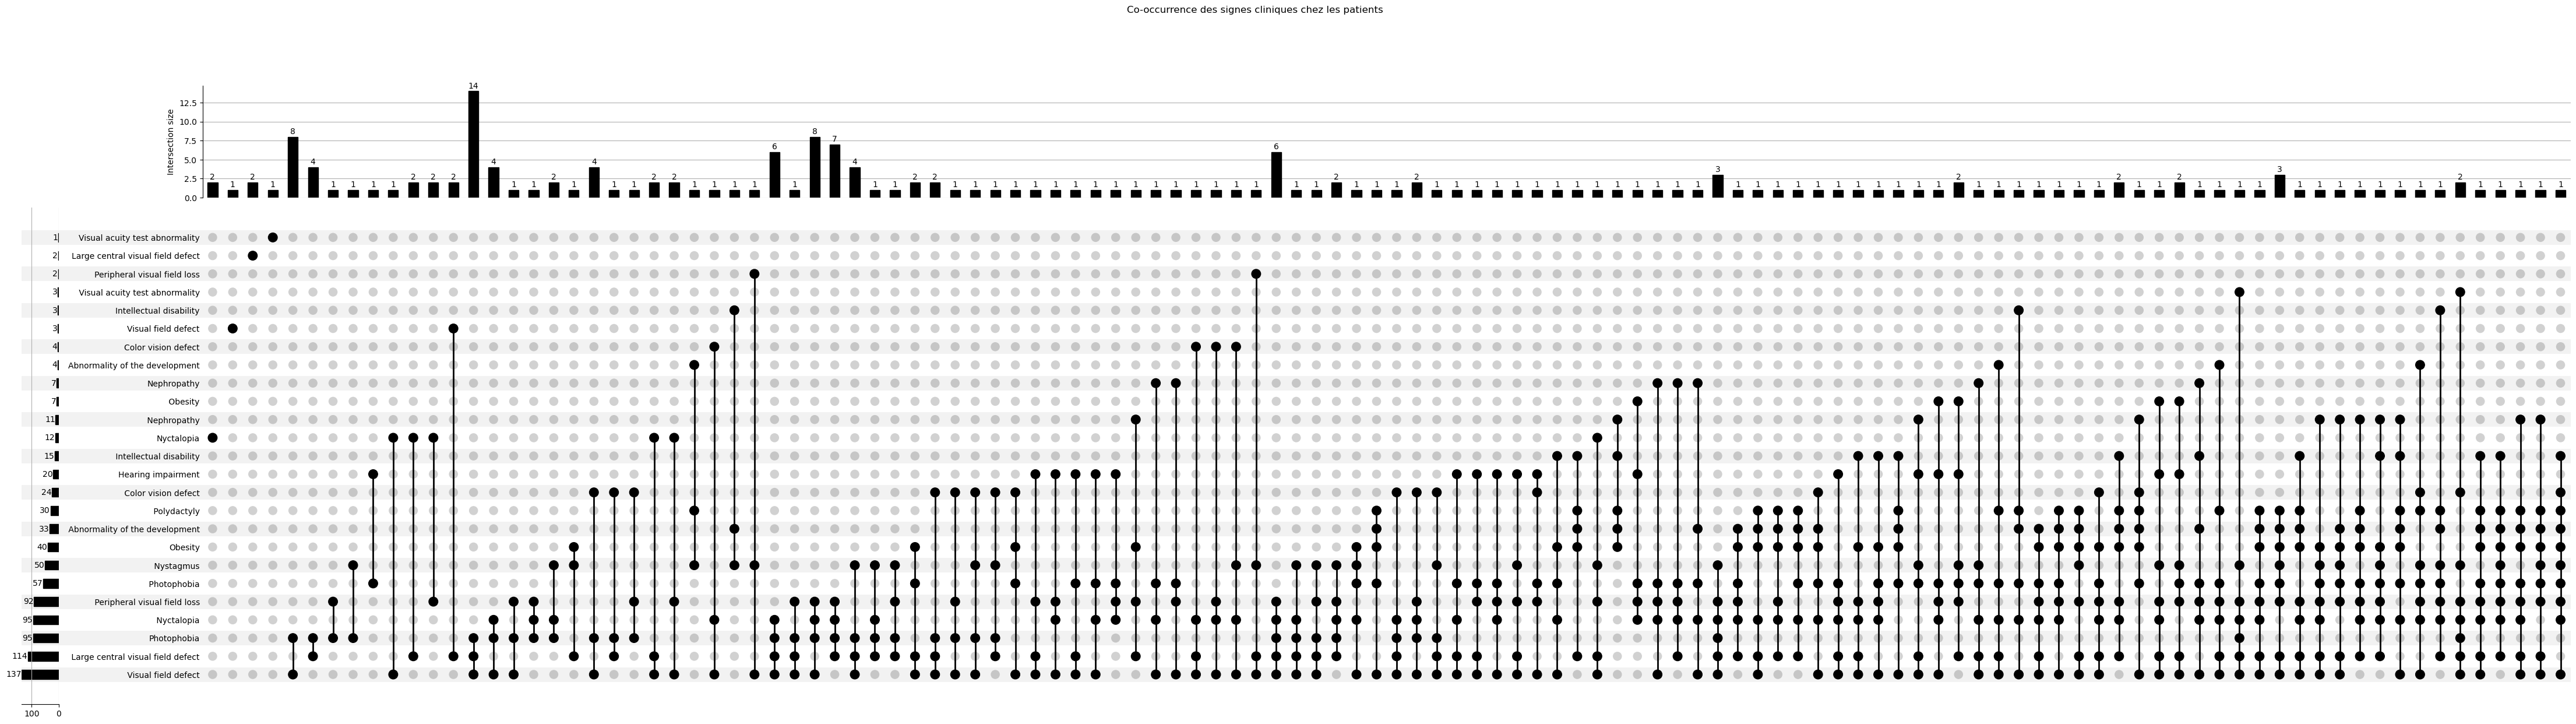
\includegraphics[keepaspectratio]{project_Fredd_files/figure-pdf/cell-77-output-2.png}}

\paragraph{3.6.5 Investigation cliniques
réalisées}\label{investigation-cliniques-ruxe9alisuxe9es}

\begin{Shaded}
\begin{Highlighting}[]
\ImportTok{from}\NormalTok{ plotly.subplots }\ImportTok{import}\NormalTok{ make\_subplots}
\ImportTok{import}\NormalTok{ plotly.graph\_objects }\ImportTok{as}\NormalTok{ go}

\NormalTok{variables }\OperatorTok{=}\NormalTok{ [}
    \StringTok{\textquotesingle{}diaCli\_invesCli\textquotesingle{}}\NormalTok{, }\StringTok{\textquotesingle{}diaCli\_invesBio\textquotesingle{}}\NormalTok{, }\StringTok{\textquotesingle{}diaCli\_invesBiol\textquotesingle{}}\NormalTok{, }\StringTok{\textquotesingle{}diaCli\_invesIma\textquotesingle{}}\NormalTok{,}
    \StringTok{\textquotesingle{}diaCli\_invesExp\textquotesingle{}}\NormalTok{, }\StringTok{\textquotesingle{}diaCli\_invesAna\textquotesingle{}}\NormalTok{, }\StringTok{\textquotesingle{}diaCli\_invesGen\textquotesingle{}}\NormalTok{, }\StringTok{\textquotesingle{}diaCli\_invesERG\textquotesingle{}}\NormalTok{, }\StringTok{\textquotesingle{}diaCli\_invesAut\textquotesingle{}}
\NormalTok{]}

\NormalTok{fig }\OperatorTok{=}\NormalTok{ make\_subplots(}
\NormalTok{    rows}\OperatorTok{=}\DecValTok{3}\NormalTok{, cols}\OperatorTok{=}\DecValTok{3}\NormalTok{,}
\NormalTok{    subplot\_titles}\OperatorTok{=}\NormalTok{variables,}
\NormalTok{    specs}\OperatorTok{=}\NormalTok{[[\{}\StringTok{"type"}\NormalTok{: }\StringTok{"domain"}\NormalTok{\}]}\OperatorTok{*}\DecValTok{3}\NormalTok{]}\OperatorTok{*}\DecValTok{3}
\NormalTok{)}

\NormalTok{couleurs }\OperatorTok{=}\NormalTok{ \{}
    \StringTok{\textquotesingle{}1\textquotesingle{}}\NormalTok{: }\StringTok{\textquotesingle{}green\textquotesingle{}}\NormalTok{,}
    \StringTok{\textquotesingle{}2\textquotesingle{}}\NormalTok{: }\StringTok{\textquotesingle{}firebrick\textquotesingle{}}\NormalTok{,}
    \StringTok{\textquotesingle{}nan\textquotesingle{}}\NormalTok{: }\StringTok{\textquotesingle{}lightgrey\textquotesingle{}}\NormalTok{,}
    \StringTok{\textquotesingle{}Genetic test\textquotesingle{}}\NormalTok{ : }\StringTok{\textquotesingle{}royalblue\textquotesingle{}}\NormalTok{,}
    \StringTok{\textquotesingle{}test de performance\textquotesingle{}}\NormalTok{ : }\StringTok{\textquotesingle{}yellow\textquotesingle{}}\NormalTok{,}
\NormalTok{\}}

\ControlFlowTok{for}\NormalTok{ i, col }\KeywordTok{in} \BuiltInTok{enumerate}\NormalTok{(variables):}
\NormalTok{    counts }\OperatorTok{=}\NormalTok{ data2[col].value\_counts(dropna}\OperatorTok{=}\VariableTok{False}\NormalTok{).reset\_index()}
\NormalTok{    counts.columns }\OperatorTok{=}\NormalTok{ [}\StringTok{\textquotesingle{}category\textquotesingle{}}\NormalTok{, }\StringTok{\textquotesingle{}count\textquotesingle{}}\NormalTok{]}
\NormalTok{    totals\_counts }\OperatorTok{=}\NormalTok{ counts[}\StringTok{\textquotesingle{}count\textquotesingle{}}\NormalTok{].}\BuiltInTok{sum}\NormalTok{()}
\NormalTok{    counts[}\StringTok{\textquotesingle{}Percentage\textquotesingle{}}\NormalTok{] }\OperatorTok{=}\NormalTok{ (counts[}\StringTok{\textquotesingle{}count\textquotesingle{}}\NormalTok{] }\OperatorTok{/}\NormalTok{ totals\_counts }\OperatorTok{*} \DecValTok{100}\NormalTok{).}\BuiltInTok{round}\NormalTok{(}\DecValTok{1}\NormalTok{)}
\NormalTok{    counts[}\StringTok{\textquotesingle{}category\textquotesingle{}}\NormalTok{] }\OperatorTok{=}\NormalTok{ counts[}\StringTok{\textquotesingle{}category\textquotesingle{}}\NormalTok{].astype(}\BuiltInTok{str}\NormalTok{)}
\NormalTok{    counts[}\StringTok{\textquotesingle{}label\textquotesingle{}}\NormalTok{] }\OperatorTok{=}\NormalTok{ counts[}\StringTok{\textquotesingle{}category\textquotesingle{}}\NormalTok{].replace(\{}\StringTok{\textquotesingle{}1\textquotesingle{}}\NormalTok{: }\StringTok{\textquotesingle{}Yes\textquotesingle{}}\NormalTok{, }\StringTok{\textquotesingle{}2\textquotesingle{}}\NormalTok{: }\StringTok{\textquotesingle{}No\textquotesingle{}}\NormalTok{, }\StringTok{\textquotesingle{}nan\textquotesingle{}}\NormalTok{: }\StringTok{\textquotesingle{}Unknown\textquotesingle{}}\NormalTok{\})}

\NormalTok{    pie }\OperatorTok{=}\NormalTok{ go.Pie(}
\NormalTok{        labels}\OperatorTok{=}\NormalTok{counts[}\StringTok{\textquotesingle{}label\textquotesingle{}}\NormalTok{],}
\NormalTok{        values}\OperatorTok{=}\NormalTok{counts[}\StringTok{\textquotesingle{}count\textquotesingle{}}\NormalTok{],}
\NormalTok{        marker\_colors}\OperatorTok{=}\NormalTok{[couleurs.get(x, }\StringTok{\textquotesingle{}grey\textquotesingle{}}\NormalTok{) }\ControlFlowTok{for}\NormalTok{ x }\KeywordTok{in}\NormalTok{ counts[}\StringTok{\textquotesingle{}category\textquotesingle{}}\NormalTok{]],}
\NormalTok{        textinfo}\OperatorTok{=}\StringTok{\textquotesingle{}percent+label+value\textquotesingle{}}\NormalTok{,}
\NormalTok{        showlegend}\OperatorTok{=}\VariableTok{False}  
\NormalTok{    )}

\NormalTok{    row }\OperatorTok{=}\NormalTok{ i }\OperatorTok{//} \DecValTok{3} \OperatorTok{+} \DecValTok{1}
\NormalTok{    col\_idx }\OperatorTok{=}\NormalTok{ i }\OperatorTok{\%} \DecValTok{3} \OperatorTok{+} \DecValTok{1}
\NormalTok{    fig.add\_trace(pie, row}\OperatorTok{=}\NormalTok{row, col}\OperatorTok{=}\NormalTok{col\_idx)}

\NormalTok{fig.update\_layout(}
\NormalTok{    height}\OperatorTok{=}\DecValTok{700}\NormalTok{, width}\OperatorTok{=}\DecValTok{800}\NormalTok{,}
\NormalTok{    title\_text}\OperatorTok{=}\StringTok{"\textless{}b\textgreater{} Investigation cliniques réalisées"}
\NormalTok{)}
\NormalTok{fig.show()}
\end{Highlighting}
\end{Shaded}

\begin{verbatim}
Unable to display output for mime type(s): text/html
\end{verbatim}

\subsubsection{3.7 Informations du test
génétique}\label{informations-du-test-guxe9nuxe9tique-1}

\paragraph{3.7.1 Listes des techniques pour le test
génétique}\label{listes-des-techniques-pour-le-test-guxe9nuxe9tique-1}

\begin{Shaded}
\begin{Highlighting}[]
\NormalTok{counts }\OperatorTok{=}\NormalTok{ data2[}\StringTok{\textquotesingle{}diaGen\_liste\_tec\textquotesingle{}}\NormalTok{].value\_counts(dropna}\OperatorTok{=}\VariableTok{False}\NormalTok{).reset\_index()}
\NormalTok{counts.columns }\OperatorTok{=}\NormalTok{ [}\StringTok{\textquotesingle{}category\textquotesingle{}}\NormalTok{, }\StringTok{\textquotesingle{}count\textquotesingle{}}\NormalTok{]}
\NormalTok{totals\_counts }\OperatorTok{=}\NormalTok{ counts[}\StringTok{\textquotesingle{}count\textquotesingle{}}\NormalTok{].}\BuiltInTok{sum}\NormalTok{()}
\NormalTok{counts[}\StringTok{\textquotesingle{}Percentage\textquotesingle{}}\NormalTok{] }\OperatorTok{=}\NormalTok{ (counts[}\StringTok{\textquotesingle{}count\textquotesingle{}}\NormalTok{] }\OperatorTok{/}\NormalTok{ totals\_counts }\OperatorTok{*} \DecValTok{100}\NormalTok{).}\BuiltInTok{round}\NormalTok{(}\DecValTok{1}\NormalTok{)}

\NormalTok{counts[}\StringTok{\textquotesingle{}category\textquotesingle{}}\NormalTok{] }\OperatorTok{=}\NormalTok{ counts[}\StringTok{\textquotesingle{}category\textquotesingle{}}\NormalTok{].astype(}\BuiltInTok{str}\NormalTok{)}
\NormalTok{counts[}\StringTok{\textquotesingle{}label\textquotesingle{}}\NormalTok{] }\OperatorTok{=}\NormalTok{ counts[}\StringTok{\textquotesingle{}category\textquotesingle{}}\NormalTok{].replace(\{}\StringTok{\textquotesingle{}1.0\textquotesingle{}}\NormalTok{: }\StringTok{\textquotesingle{}Séquençage SANGER simple\textquotesingle{}}\NormalTok{, }
                                              \StringTok{\textquotesingle{}2.0\textquotesingle{}}\NormalTok{: }\StringTok{\textquotesingle{}Séquençage ciblé avec panel de 10{-}30 gènes\textquotesingle{}}\NormalTok{, }
                                              \StringTok{\textquotesingle{}5.0\textquotesingle{}}\NormalTok{: }\StringTok{\textquotesingle{}PCR Quantitative\textquotesingle{}}\NormalTok{, }
                                              \StringTok{\textquotesingle{}6.0\textquotesingle{}}\NormalTok{: }\StringTok{\textquotesingle{}Séquençage exome entier (WES)\textquotesingle{}}\NormalTok{,}
                                              \StringTok{\textquotesingle{}7.0\textquotesingle{}}\NormalTok{: }\StringTok{\textquotesingle{}Séquençage génome entier (WGS)\textquotesingle{}}\NormalTok{, }
                                              \StringTok{\textquotesingle{}9.0\textquotesingle{}}\NormalTok{: }\StringTok{\textquotesingle{}Others\textquotesingle{}}\NormalTok{,}
                                              \StringTok{\textquotesingle{}nan\textquotesingle{}}\NormalTok{: }\StringTok{\textquotesingle{}Unknown\textquotesingle{}}\NormalTok{\})}


\NormalTok{fig }\OperatorTok{=}\NormalTok{ px.pie(}
\NormalTok{        counts,}
\NormalTok{        names}\OperatorTok{=}\StringTok{\textquotesingle{}label\textquotesingle{}}\NormalTok{,}
\NormalTok{        values}\OperatorTok{=}\StringTok{\textquotesingle{}count\textquotesingle{}}\NormalTok{,}
\NormalTok{        title}\OperatorTok{=}\SpecialStringTok{f"\textless{}b\textgreater{}Méthode utilisées pour le test génétique"}\NormalTok{,}
        \CommentTok{\# pull=[0, 0, 0, 0.2, 0, 0],}
\NormalTok{        color\_discrete\_sequence}\OperatorTok{=}\NormalTok{px.colors.qualitative.Bold}

\NormalTok{    )}
\NormalTok{fig.update\_traces(textposition}\OperatorTok{=}\StringTok{\textquotesingle{}auto\textquotesingle{}}\NormalTok{, textinfo}\OperatorTok{=}\StringTok{\textquotesingle{}percent+label+value\textquotesingle{}}\NormalTok{)}

\NormalTok{fig.show()}
\end{Highlighting}
\end{Shaded}

\begin{verbatim}
Unable to display output for mime type(s): text/html
\end{verbatim}

\paragraph{3.7.2 Statut du dernier test
genetique}\label{statut-du-dernier-test-genetique}

\begin{Shaded}
\begin{Highlighting}[]
\NormalTok{counts }\OperatorTok{=}\NormalTok{ data2[}\StringTok{\textquotesingle{}diaGen\_statut\_analyse\textquotesingle{}}\NormalTok{].value\_counts(dropna}\OperatorTok{=}\VariableTok{False}\NormalTok{).reset\_index()}
\NormalTok{counts.columns }\OperatorTok{=}\NormalTok{ [}\StringTok{\textquotesingle{}category\textquotesingle{}}\NormalTok{, }\StringTok{\textquotesingle{}count\textquotesingle{}}\NormalTok{]}
\NormalTok{totals\_counts }\OperatorTok{=}\NormalTok{ counts[}\StringTok{\textquotesingle{}count\textquotesingle{}}\NormalTok{].}\BuiltInTok{sum}\NormalTok{()}
\NormalTok{counts[}\StringTok{\textquotesingle{}Percentage\textquotesingle{}}\NormalTok{] }\OperatorTok{=}\NormalTok{ (counts[}\StringTok{\textquotesingle{}count\textquotesingle{}}\NormalTok{] }\OperatorTok{/}\NormalTok{ totals\_counts }\OperatorTok{*} \DecValTok{100}\NormalTok{).}\BuiltInTok{round}\NormalTok{(}\DecValTok{1}\NormalTok{)}

\NormalTok{counts[}\StringTok{\textquotesingle{}category\textquotesingle{}}\NormalTok{] }\OperatorTok{=}\NormalTok{ counts[}\StringTok{\textquotesingle{}category\textquotesingle{}}\NormalTok{].astype(}\BuiltInTok{str}\NormalTok{)}
\NormalTok{counts[}\StringTok{\textquotesingle{}label\textquotesingle{}}\NormalTok{] }\OperatorTok{=}\NormalTok{ counts[}\StringTok{\textquotesingle{}category\textquotesingle{}}\NormalTok{].replace(\{}\StringTok{\textquotesingle{}1\textquotesingle{}}\NormalTok{: }\StringTok{\textquotesingle{}En cours\textquotesingle{}}\NormalTok{, }
                                              \StringTok{\textquotesingle{}2\textquotesingle{}}\NormalTok{: }\StringTok{\textquotesingle{}Terminé\textquotesingle{}}\NormalTok{,}
                                              \StringTok{\textquotesingle{}3\textquotesingle{}}\NormalTok{: }\StringTok{\textquotesingle{}Indéterminé\textquotesingle{}}
\NormalTok{                                             \})}

\NormalTok{fig }\OperatorTok{=}\NormalTok{ px.pie(}
\NormalTok{        counts,}
\NormalTok{        names}\OperatorTok{=}\StringTok{\textquotesingle{}label\textquotesingle{}}\NormalTok{,}
\NormalTok{        values}\OperatorTok{=}\StringTok{\textquotesingle{}count\textquotesingle{}}\NormalTok{,}
\NormalTok{        title}\OperatorTok{=}\SpecialStringTok{f"\textless{}b\textgreater{}Statut du dernier test"}\NormalTok{,}
\NormalTok{        color\_discrete\_sequence}\OperatorTok{=}\NormalTok{px.colors.qualitative.Bold}

\NormalTok{    )}
\NormalTok{fig.update\_traces(textposition}\OperatorTok{=}\StringTok{\textquotesingle{}inside\textquotesingle{}}\NormalTok{, textinfo}\OperatorTok{=}\StringTok{\textquotesingle{}percent+label+value\textquotesingle{}}\NormalTok{)}

\NormalTok{fig.show()}
\end{Highlighting}
\end{Shaded}

\begin{verbatim}
Unable to display output for mime type(s): text/html
\end{verbatim}

\paragraph{3.7.3 Patients n'ayant pas de date du dernier test avec le
statut
confirmé}\label{patients-nayant-pas-de-date-du-dernier-test-avec-le-statut-confirmuxe9}

\begin{Shaded}
\begin{Highlighting}[]
\NormalTok{data2[(data2[}\StringTok{\textquotesingle{}diaGen\_CR\_date\textquotesingle{}}\NormalTok{].isna()) }\OperatorTok{\&}\NormalTok{ (data2[}\StringTok{\textquotesingle{}diaGen\_statut\_analyse\textquotesingle{}}\NormalTok{] }\OperatorTok{==} \DecValTok{2}\NormalTok{)][}
\NormalTok{[}\StringTok{\textquotesingle{}adm\_date\_naissance\textquotesingle{}}\NormalTok{, }\StringTok{\textquotesingle{}diaGen\_statut\_analyse\textquotesingle{}}\NormalTok{, }\StringTok{\textquotesingle{}diaGen\_CR\_date\textquotesingle{}}\NormalTok{, }\StringTok{\textquotesingle{}diaGen\_var\_hgcn\_1\textquotesingle{}}\NormalTok{]]}
\end{Highlighting}
\end{Shaded}

\begin{longtable}[]{@{}lllll@{}}
\toprule\noalign{}
& adm\_date\_naissance & diaGen\_statut\_analyse & diaGen\_CR\_date &
diaGen\_var\_hgcn\_1 \\
\midrule\noalign{}
\endhead
\bottomrule\noalign{}
\endlastfoot
5 & 1958-03-05 & 2 & NaT & ABCA4 \\
86 & 1982-06-12 & 2 & NaT & ABCA4 \\
\end{longtable}

\paragraph{3.7.4 Proportions des Patients ayant 0, 1, 2
gènes}\label{proportions-des-patients-ayant-0-1-2-guxe8nes}

\begin{Shaded}
\begin{Highlighting}[]
\NormalTok{counts }\OperatorTok{=}\NormalTok{ data2[}\StringTok{\textquotesingle{}diaGen\_var\_nbgene\textquotesingle{}}\NormalTok{].value\_counts(dropna}\OperatorTok{=}\VariableTok{False}\NormalTok{).reset\_index()}
\NormalTok{counts.columns }\OperatorTok{=}\NormalTok{ [}\StringTok{\textquotesingle{}category\textquotesingle{}}\NormalTok{, }\StringTok{\textquotesingle{}count\textquotesingle{}}\NormalTok{]}
\NormalTok{totals\_counts }\OperatorTok{=}\NormalTok{ counts[}\StringTok{\textquotesingle{}count\textquotesingle{}}\NormalTok{].}\BuiltInTok{sum}\NormalTok{()}
\NormalTok{counts[}\StringTok{\textquotesingle{}Percentage\textquotesingle{}}\NormalTok{] }\OperatorTok{=}\NormalTok{ (counts[}\StringTok{\textquotesingle{}count\textquotesingle{}}\NormalTok{] }\OperatorTok{/}\NormalTok{ totals\_counts }\OperatorTok{*} \DecValTok{100}\NormalTok{).}\BuiltInTok{round}\NormalTok{(}\DecValTok{1}\NormalTok{)}

\NormalTok{counts[}\StringTok{\textquotesingle{}category\textquotesingle{}}\NormalTok{] }\OperatorTok{=}\NormalTok{ counts[}\StringTok{\textquotesingle{}category\textquotesingle{}}\NormalTok{].astype(}\BuiltInTok{str}\NormalTok{)}
\NormalTok{counts[}\StringTok{\textquotesingle{}label\textquotesingle{}}\NormalTok{] }\OperatorTok{=}\NormalTok{ counts[}\StringTok{\textquotesingle{}category\textquotesingle{}}\NormalTok{].replace(\{}\StringTok{\textquotesingle{}0\textquotesingle{}}\NormalTok{ : }\StringTok{\textquotesingle{}0 gene\textquotesingle{}}\NormalTok{, }\StringTok{\textquotesingle{}1\textquotesingle{}}\NormalTok{ : }\StringTok{\textquotesingle{}1 gene\textquotesingle{}}\NormalTok{, }\StringTok{\textquotesingle{}2\textquotesingle{}}\NormalTok{ : }\StringTok{\textquotesingle{}2 gene\textquotesingle{}}\NormalTok{\})}


\NormalTok{fig }\OperatorTok{=}\NormalTok{ px.pie(}
\NormalTok{        counts,}
\NormalTok{        names}\OperatorTok{=}\StringTok{\textquotesingle{}label\textquotesingle{}}\NormalTok{,}
\NormalTok{        values}\OperatorTok{=}\StringTok{\textquotesingle{}count\textquotesingle{}}\NormalTok{,}
\NormalTok{        title}\OperatorTok{=}\SpecialStringTok{f"\textless{}b\textgreater{} Nombre de patients ayant 0, 1, 2 gènes"}\NormalTok{,}
\NormalTok{        color\_discrete\_sequence}\OperatorTok{=}\NormalTok{px.colors.qualitative.Bold}

\NormalTok{    )}
\NormalTok{fig.update\_traces(textposition}\OperatorTok{=}\StringTok{\textquotesingle{}auto\textquotesingle{}}\NormalTok{, textinfo}\OperatorTok{=}\StringTok{\textquotesingle{}percent+label+value\textquotesingle{}}\NormalTok{)}

\NormalTok{fig.show()}
\end{Highlighting}
\end{Shaded}

\begin{verbatim}
Unable to display output for mime type(s): text/html
\end{verbatim}

\paragraph{3.7.5 Listes des Gènes
repertoriés}\label{listes-des-guxe8nes-repertoriuxe9s-1}

\begin{Shaded}
\begin{Highlighting}[]
\ImportTok{import}\NormalTok{ plotly.express }\ImportTok{as}\NormalTok{ px}
\ImportTok{import}\NormalTok{ pandas }\ImportTok{as}\NormalTok{ pd}

\NormalTok{diagnosis\_counts }\OperatorTok{=}\NormalTok{ data2[}\StringTok{\textquotesingle{}diaGen\_var\_hgcn\_1\textquotesingle{}}\NormalTok{].value\_counts().reset\_index()}
\NormalTok{diagnosis\_counts.columns }\OperatorTok{=}\NormalTok{ [}\StringTok{\textquotesingle{}Diagnosis\textquotesingle{}}\NormalTok{, }\StringTok{\textquotesingle{}Number of cases\textquotesingle{}}\NormalTok{]}

\NormalTok{total\_patients }\OperatorTok{=}\NormalTok{ diagnosis\_counts[}\StringTok{\textquotesingle{}Number of cases\textquotesingle{}}\NormalTok{].}\BuiltInTok{sum}\NormalTok{()}
\NormalTok{diagnosis\_counts[}\StringTok{\textquotesingle{}Percentage\textquotesingle{}}\NormalTok{] }\OperatorTok{=}\NormalTok{ (diagnosis\_counts[}\StringTok{\textquotesingle{}Number of cases\textquotesingle{}}\NormalTok{] }\OperatorTok{/}\NormalTok{ total\_patients }\OperatorTok{*} \DecValTok{100}\NormalTok{).}\BuiltInTok{round}\NormalTok{(}\DecValTok{1}\NormalTok{)}

\NormalTok{fig }\OperatorTok{=}\NormalTok{ px.bar(}
\NormalTok{    diagnosis\_counts,}
\NormalTok{    x}\OperatorTok{=}\StringTok{\textquotesingle{}Diagnosis\textquotesingle{}}\NormalTok{,}
\NormalTok{    y}\OperatorTok{=}\StringTok{\textquotesingle{}Number of cases\textquotesingle{}}\NormalTok{,}
\NormalTok{    color}\OperatorTok{=}\StringTok{\textquotesingle{}Number of cases\textquotesingle{}}\NormalTok{,}
\NormalTok{    color\_continuous\_scale}\OperatorTok{=}\StringTok{\textquotesingle{}Plasma\textquotesingle{}}\NormalTok{,}
\NormalTok{    text}\OperatorTok{=}\StringTok{\textquotesingle{}Number of cases\textquotesingle{}}\NormalTok{,  }
\NormalTok{    title}\OperatorTok{=}\StringTok{\textquotesingle{}\textless{}b\textgreater{}Distribution du nombre de gènes  diagnosis\textless{}/b\textgreater{}\textquotesingle{}}\NormalTok{,}
\NormalTok{    labels}\OperatorTok{=}\NormalTok{\{}\StringTok{\textquotesingle{}Number of cases\textquotesingle{}}\NormalTok{: }\StringTok{\textquotesingle{}Nb cases\textquotesingle{}}\NormalTok{, }\StringTok{\textquotesingle{}Diagnosis\textquotesingle{}}\NormalTok{: }\StringTok{\textquotesingle{}Genes\textquotesingle{}}\NormalTok{\},}
\NormalTok{    height}\OperatorTok{=}\DecValTok{900}
\NormalTok{)}

\NormalTok{fig.update\_layout(}
\NormalTok{    xaxis}\OperatorTok{=}\NormalTok{\{}\StringTok{\textquotesingle{}categoryorder\textquotesingle{}}\NormalTok{:}\StringTok{\textquotesingle{}total descending\textquotesingle{}}\NormalTok{\},}
\NormalTok{    plot\_bgcolor}\OperatorTok{=}\StringTok{\textquotesingle{}rgba(0,0,0,0)\textquotesingle{}}\NormalTok{,}
\NormalTok{    hovermode}\OperatorTok{=}\StringTok{\textquotesingle{}x unified\textquotesingle{}}\NormalTok{,}
\NormalTok{    title\_font}\OperatorTok{=}\NormalTok{\{}\StringTok{\textquotesingle{}size\textquotesingle{}}\NormalTok{: }\DecValTok{20}\NormalTok{\},}
\NormalTok{    uniformtext\_minsize}\OperatorTok{=}\DecValTok{8}
\NormalTok{)}

\NormalTok{fig.update\_traces(}
\NormalTok{    texttemplate}\OperatorTok{=}\StringTok{\textquotesingle{}\textless{}b\textgreater{}\%}\SpecialCharTok{\{y\}}\StringTok{\textless{}/b\textgreater{}\textless{}br\textgreater{}(\%}\SpecialCharTok{\{customdata[0]\}}\StringTok{\%)\textquotesingle{}}\NormalTok{,}
\NormalTok{    hovertemplate}\OperatorTok{=}\StringTok{"\textless{}b\textgreater{}\%}\SpecialCharTok{\{x\}}\StringTok{\textless{}/b\textgreater{}\textless{}br\textgreater{}Cases: \%}\SpecialCharTok{\{y\}}\StringTok{\textless{}br\textgreater{}Proportion: \%}\SpecialCharTok{\{customdata[0]\}}\StringTok{\%"}\NormalTok{,}
\NormalTok{    textposition}\OperatorTok{=}\StringTok{\textquotesingle{}outside\textquotesingle{}}\NormalTok{,}
\NormalTok{    customdata}\OperatorTok{=}\NormalTok{diagnosis\_counts[[}\StringTok{\textquotesingle{}Percentage\textquotesingle{}}\NormalTok{]]}
\NormalTok{)}

\NormalTok{fig.show()}
\end{Highlighting}
\end{Shaded}

\begin{verbatim}
Unable to display output for mime type(s): text/html
\end{verbatim}

\paragraph{3.7.6 Méthodes de transmission de
gènes}\label{muxe9thodes-de-transmission-de-guxe8nes-1}

\begin{Shaded}
\begin{Highlighting}[]
\NormalTok{counts }\OperatorTok{=}\NormalTok{ data2[}\StringTok{\textquotesingle{}diaGen\_var\_trans\_1\textquotesingle{}}\NormalTok{].value\_counts(dropna}\OperatorTok{=}\VariableTok{False}\NormalTok{).reset\_index()}
\NormalTok{counts.columns }\OperatorTok{=}\NormalTok{ [}\StringTok{\textquotesingle{}category\textquotesingle{}}\NormalTok{, }\StringTok{\textquotesingle{}count\textquotesingle{}}\NormalTok{]}
\NormalTok{totals\_counts }\OperatorTok{=}\NormalTok{ counts[}\StringTok{\textquotesingle{}count\textquotesingle{}}\NormalTok{].}\BuiltInTok{sum}\NormalTok{()}
\NormalTok{counts[}\StringTok{\textquotesingle{}Percentage\textquotesingle{}}\NormalTok{] }\OperatorTok{=}\NormalTok{ (counts[}\StringTok{\textquotesingle{}count\textquotesingle{}}\NormalTok{] }\OperatorTok{/}\NormalTok{ totals\_counts }\OperatorTok{*} \DecValTok{100}\NormalTok{).}\BuiltInTok{round}\NormalTok{(}\DecValTok{1}\NormalTok{)}

\NormalTok{counts[}\StringTok{\textquotesingle{}category\textquotesingle{}}\NormalTok{] }\OperatorTok{=}\NormalTok{ counts[}\StringTok{\textquotesingle{}category\textquotesingle{}}\NormalTok{].astype(}\BuiltInTok{str}\NormalTok{)}
\NormalTok{counts[}\StringTok{\textquotesingle{}label\textquotesingle{}}\NormalTok{] }\OperatorTok{=}\NormalTok{ counts[}\StringTok{\textquotesingle{}category\textquotesingle{}}\NormalTok{].replace(\{}\StringTok{\textquotesingle{}1.0\textquotesingle{}}\NormalTok{: }\StringTok{\textquotesingle{}De novo\textquotesingle{}}\NormalTok{, }\StringTok{\textquotesingle{}2.0\textquotesingle{}}\NormalTok{: }\StringTok{\textquotesingle{}Autosomique dominant\textquotesingle{}}\NormalTok{, }
                                              \StringTok{\textquotesingle{}3.0\textquotesingle{}}\NormalTok{: }\StringTok{\textquotesingle{}Autosomique récessif\textquotesingle{}}\NormalTok{, }\StringTok{\textquotesingle{}nan\textquotesingle{}}\NormalTok{: }\StringTok{\textquotesingle{}Unknown\textquotesingle{}}\NormalTok{\})}


\NormalTok{fig }\OperatorTok{=}\NormalTok{ px.pie(}
\NormalTok{        counts,}
\NormalTok{        names}\OperatorTok{=}\StringTok{\textquotesingle{}label\textquotesingle{}}\NormalTok{,}
\NormalTok{        values}\OperatorTok{=}\StringTok{\textquotesingle{}count\textquotesingle{}}\NormalTok{,}
\NormalTok{        title}\OperatorTok{=}\SpecialStringTok{f"\textless{}b\textgreater{} Méthode de transmission"}\NormalTok{,}
\NormalTok{        color\_discrete\_sequence}\OperatorTok{=}\NormalTok{px.colors.qualitative.Bold}

\NormalTok{    )}
\NormalTok{fig.update\_traces(textposition}\OperatorTok{=}\StringTok{\textquotesingle{}inside\textquotesingle{}}\NormalTok{, textinfo}\OperatorTok{=}\StringTok{\textquotesingle{}percent+label+value\textquotesingle{}}\NormalTok{)}

\NormalTok{fig.show()}
\end{Highlighting}
\end{Shaded}

\begin{verbatim}
Unable to display output for mime type(s): text/html
\end{verbatim}

\subsubsection{3.8 Correlation
Genotype/Phenotype}\label{correlation-genotypephenotype}

\begin{Shaded}
\begin{Highlighting}[]
\NormalTok{counts }\OperatorTok{=}\NormalTok{ data2[}\StringTok{\textquotesingle{}diaGen\_corr\textquotesingle{}}\NormalTok{].value\_counts(dropna}\OperatorTok{=}\VariableTok{False}\NormalTok{).reset\_index()}
\NormalTok{counts.columns }\OperatorTok{=}\NormalTok{ [}\StringTok{\textquotesingle{}category\textquotesingle{}}\NormalTok{, }\StringTok{\textquotesingle{}count\textquotesingle{}}\NormalTok{]}
\NormalTok{totals\_counts }\OperatorTok{=}\NormalTok{ counts[}\StringTok{\textquotesingle{}count\textquotesingle{}}\NormalTok{].}\BuiltInTok{sum}\NormalTok{()}
\NormalTok{counts[}\StringTok{\textquotesingle{}Percentage\textquotesingle{}}\NormalTok{] }\OperatorTok{=}\NormalTok{ (counts[}\StringTok{\textquotesingle{}count\textquotesingle{}}\NormalTok{] }\OperatorTok{/}\NormalTok{ totals\_counts }\OperatorTok{*} \DecValTok{100}\NormalTok{).}\BuiltInTok{round}\NormalTok{(}\DecValTok{1}\NormalTok{)}

\NormalTok{counts[}\StringTok{\textquotesingle{}category\textquotesingle{}}\NormalTok{] }\OperatorTok{=}\NormalTok{ counts[}\StringTok{\textquotesingle{}category\textquotesingle{}}\NormalTok{].astype(}\BuiltInTok{str}\NormalTok{)}
\NormalTok{counts[}\StringTok{\textquotesingle{}label\textquotesingle{}}\NormalTok{] }\OperatorTok{=}\NormalTok{ counts[}\StringTok{\textquotesingle{}category\textquotesingle{}}\NormalTok{].replace(\{}\StringTok{\textquotesingle{}1.0\textquotesingle{}}\NormalTok{: }\StringTok{\textquotesingle{}Yes(classical case)\textquotesingle{}}\NormalTok{,  }
                                              \StringTok{\textquotesingle{}0.0\textquotesingle{}}\NormalTok{: }\StringTok{\textquotesingle{}No(atypic case) \textquotesingle{}}\NormalTok{, }
                                              \StringTok{\textquotesingle{}nan\textquotesingle{}}\NormalTok{: }\StringTok{\textquotesingle{}Unknown\textquotesingle{}}\NormalTok{\})}


\NormalTok{fig }\OperatorTok{=}\NormalTok{ px.pie(}
\NormalTok{        counts,}
\NormalTok{        names}\OperatorTok{=}\StringTok{\textquotesingle{}label\textquotesingle{}}\NormalTok{,}
\NormalTok{        values}\OperatorTok{=}\StringTok{\textquotesingle{}count\textquotesingle{}}\NormalTok{,}
\NormalTok{        title}\OperatorTok{=}\SpecialStringTok{f"\textless{}b\textgreater{}Correlation Genotype/Phenotype"}\NormalTok{,}
\NormalTok{        color\_discrete\_sequence}\OperatorTok{=}\NormalTok{px.colors.qualitative.Bold}

\NormalTok{    )}
\NormalTok{fig.update\_traces(textposition}\OperatorTok{=}\StringTok{\textquotesingle{}inside\textquotesingle{}}\NormalTok{, textinfo}\OperatorTok{=}\StringTok{\textquotesingle{}percent+label\textquotesingle{}}\NormalTok{)}

\NormalTok{fig.show()}
\end{Highlighting}
\end{Shaded}

\begin{verbatim}
Unable to display output for mime type(s): text/html
\end{verbatim}

\begin{Shaded}
\begin{Highlighting}[]
\ImportTok{import}\NormalTok{ seaborn }\ImportTok{as}\NormalTok{ sns}
\ImportTok{import}\NormalTok{ matplotlib.pyplot }\ImportTok{as}\NormalTok{ plt}

\NormalTok{pivot }\OperatorTok{=}\NormalTok{ data2.pivot\_table(}
\NormalTok{    index}\OperatorTok{=}\StringTok{\textquotesingle{}diaCli\_diagMR\_nom\textquotesingle{}}\NormalTok{,}
\NormalTok{    columns}\OperatorTok{=}\StringTok{\textquotesingle{}diaGen\_var\_hgcn\_1\textquotesingle{}}\NormalTok{,}
\NormalTok{    aggfunc}\OperatorTok{=}\StringTok{\textquotesingle{}size\textquotesingle{}}\NormalTok{,}
\NormalTok{    fill\_value}\OperatorTok{=}\DecValTok{0}
\NormalTok{)}

\NormalTok{plt.figure(figsize}\OperatorTok{=}\NormalTok{(}\DecValTok{18}\NormalTok{, }\DecValTok{10}\NormalTok{))}
\NormalTok{sns.heatmap(pivot, cmap}\OperatorTok{=}\StringTok{\textquotesingle{}YlGnBu\textquotesingle{}}\NormalTok{, annot}\OperatorTok{=}\VariableTok{True}\NormalTok{, fmt}\OperatorTok{=}\StringTok{"d"}\NormalTok{)}
\NormalTok{plt.title(}\StringTok{"Fréquence des combinaisons Diagnostic {-} Gène"}\NormalTok{)}
\NormalTok{plt.ylabel(}\StringTok{"Diagnostic"}\NormalTok{)}
\NormalTok{plt.xlabel(}\StringTok{"Gène identifié"}\NormalTok{)}
\NormalTok{plt.tight\_layout()}
\NormalTok{plt.show()}
\end{Highlighting}
\end{Shaded}

\pandocbounded{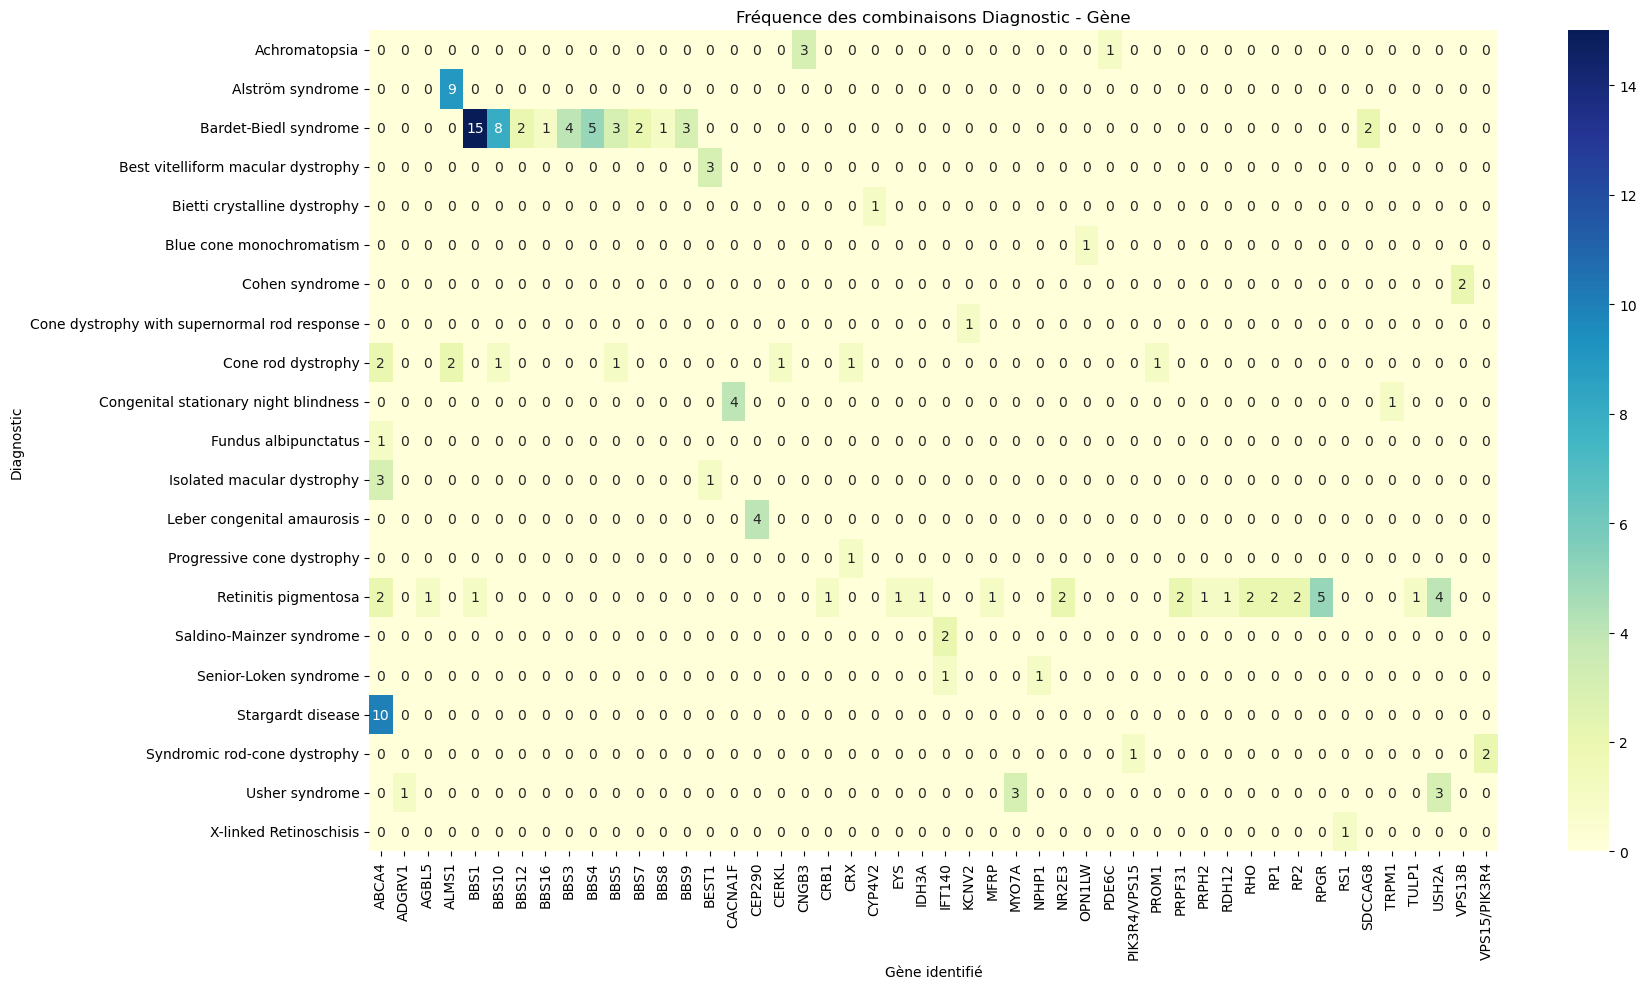
\includegraphics[keepaspectratio]{project_Fredd_files/figure-pdf/cell-86-output-1.png}}

\subsubsection{3.9 Examen Acuité
visuelle}\label{examen-acuituxe9-visuelle-1}

\begin{Shaded}
\begin{Highlighting}[]
\NormalTok{data2[}\StringTok{\textquotesingle{}exaAcu\_type\_examen\_OD\textquotesingle{}}\NormalTok{].unique()}
\end{Highlighting}
\end{Shaded}

\begin{verbatim}
array([nan,  1.,  2.,  4.])
\end{verbatim}

\begin{Shaded}
\begin{Highlighting}[]
\ImportTok{from}\NormalTok{ plotly.subplots }\ImportTok{import}\NormalTok{ make\_subplots}
\ImportTok{import}\NormalTok{ plotly.graph\_objects }\ImportTok{as}\NormalTok{ go}

\NormalTok{variables }\OperatorTok{=}\NormalTok{ [}\StringTok{\textquotesingle{}exaAcu\_type\_examen\_OG\textquotesingle{}}\NormalTok{, }\StringTok{\textquotesingle{}exaAcu\_type\_examen\_OD\textquotesingle{}}\NormalTok{]}

\NormalTok{fig }\OperatorTok{=}\NormalTok{ make\_subplots(}
\NormalTok{    rows}\OperatorTok{=}\DecValTok{1}\NormalTok{, cols}\OperatorTok{=}\DecValTok{2}\NormalTok{,}
\NormalTok{    subplot\_titles}\OperatorTok{=}\NormalTok{variables,}
\NormalTok{    specs}\OperatorTok{=}\NormalTok{[[\{}\StringTok{\textquotesingle{}type\textquotesingle{}}\NormalTok{: }\StringTok{\textquotesingle{}domain\textquotesingle{}}\NormalTok{\}, \{}\StringTok{\textquotesingle{}type\textquotesingle{}}\NormalTok{: }\StringTok{\textquotesingle{}domain\textquotesingle{}}\NormalTok{\}]]}
\NormalTok{)}

\ControlFlowTok{for}\NormalTok{ i, col }\KeywordTok{in} \BuiltInTok{enumerate}\NormalTok{(variables):}
\NormalTok{    counts }\OperatorTok{=}\NormalTok{ data2[col].value\_counts(dropna}\OperatorTok{=}\VariableTok{False}\NormalTok{).reset\_index()}
\NormalTok{    counts.columns }\OperatorTok{=}\NormalTok{ [}\StringTok{\textquotesingle{}category\textquotesingle{}}\NormalTok{, }\StringTok{\textquotesingle{}count\textquotesingle{}}\NormalTok{]}
\NormalTok{    totals\_counts }\OperatorTok{=}\NormalTok{ counts[}\StringTok{\textquotesingle{}count\textquotesingle{}}\NormalTok{].}\BuiltInTok{sum}\NormalTok{()}
\NormalTok{    counts[}\StringTok{\textquotesingle{}Percentage\textquotesingle{}}\NormalTok{] }\OperatorTok{=}\NormalTok{ (counts[}\StringTok{\textquotesingle{}count\textquotesingle{}}\NormalTok{] }\OperatorTok{/}\NormalTok{ totals\_counts }\OperatorTok{*} \DecValTok{100}\NormalTok{).}\BuiltInTok{round}\NormalTok{(}\DecValTok{1}\NormalTok{)}
\NormalTok{    counts[}\StringTok{\textquotesingle{}category\textquotesingle{}}\NormalTok{] }\OperatorTok{=}\NormalTok{ counts[}\StringTok{\textquotesingle{}category\textquotesingle{}}\NormalTok{].astype(}\BuiltInTok{str}\NormalTok{)}
\NormalTok{    counts[}\StringTok{\textquotesingle{}label\textquotesingle{}}\NormalTok{] }\OperatorTok{=}\NormalTok{ counts[}\StringTok{\textquotesingle{}category\textquotesingle{}}\NormalTok{].replace(\{}\StringTok{\textquotesingle{}1.0\textquotesingle{}}\NormalTok{: }\StringTok{\textquotesingle{}Monoyer\textquotesingle{}}\NormalTok{, }\StringTok{\textquotesingle{}2.0\textquotesingle{}}\NormalTok{: }\StringTok{\textquotesingle{}Pigassou\textquotesingle{}}\NormalTok{,}
                                                  \StringTok{\textquotesingle{}3.0\textquotesingle{}}\NormalTok{: }\StringTok{\textquotesingle{}Bébé vision\textquotesingle{}}\NormalTok{, }\StringTok{\textquotesingle{}4.0\textquotesingle{}}\NormalTok{: }\StringTok{\textquotesingle{}Cardiff\textquotesingle{}}\NormalTok{,}
                                                 \StringTok{\textquotesingle{}5.0\textquotesingle{}}\NormalTok{: }\StringTok{\textquotesingle{}EDTRS\textquotesingle{}}\NormalTok{,}\StringTok{\textquotesingle{}6.0\textquotesingle{}}\NormalTok{ : }\StringTok{\textquotesingle{}Autre\textquotesingle{}}\NormalTok{\})}
\NormalTok{    pie }\OperatorTok{=}\NormalTok{ go.Pie(}
\NormalTok{        labels}\OperatorTok{=}\NormalTok{counts[}\StringTok{\textquotesingle{}label\textquotesingle{}}\NormalTok{],}
\NormalTok{        values}\OperatorTok{=}\NormalTok{counts[}\StringTok{\textquotesingle{}count\textquotesingle{}}\NormalTok{],}
\NormalTok{        textinfo}\OperatorTok{=}\StringTok{\textquotesingle{}percent+label\textquotesingle{}}\NormalTok{,}
\NormalTok{        showlegend}\OperatorTok{=}\VariableTok{False}  
\NormalTok{    )}

\NormalTok{    row }\OperatorTok{=} \DecValTok{1}
\NormalTok{    col\_idx }\OperatorTok{=}\NormalTok{ i }\OperatorTok{+} \DecValTok{1}
\NormalTok{    fig.add\_trace(pie, row}\OperatorTok{=}\NormalTok{row, col}\OperatorTok{=}\NormalTok{col\_idx)}

\NormalTok{fig.update\_layout(}
\NormalTok{    height}\OperatorTok{=}\DecValTok{450}\NormalTok{, width}\OperatorTok{=}\DecValTok{850}\NormalTok{,}
\NormalTok{    title\_text}\OperatorTok{=}\StringTok{"\textless{}b\textgreater{}Types d\textquotesingle{}examen pour la mesure de l\textquotesingle{}acuité visuelle\textless{}/b\textgreater{}"}
\NormalTok{)}
\NormalTok{fig.update\_traces(textposition}\OperatorTok{=}\StringTok{\textquotesingle{}inside\textquotesingle{}}\NormalTok{, textinfo}\OperatorTok{=}\StringTok{\textquotesingle{}percent+label+value\textquotesingle{}}\NormalTok{)}

\NormalTok{fig.show()}
\end{Highlighting}
\end{Shaded}

\begin{verbatim}
Unable to display output for mime type(s): text/html
\end{verbatim}

\subsubsection{3.10 Examen champ visuel}\label{examen-champ-visuel-1}

\begin{Shaded}
\begin{Highlighting}[]
\NormalTok{proportions }\OperatorTok{=}\NormalTok{ data2[}\StringTok{\textquotesingle{}exaChv\_fait\textquotesingle{}}\NormalTok{].value\_counts().reset\_index()}
\NormalTok{proportions.columns }\OperatorTok{=}\NormalTok{ [}\StringTok{\textquotesingle{}exaChv\_fait\textquotesingle{}}\NormalTok{, }\StringTok{\textquotesingle{}proportion\textquotesingle{}}\NormalTok{]}
\NormalTok{totals\_counts }\OperatorTok{=}\NormalTok{ proportions[}\StringTok{\textquotesingle{}proportion\textquotesingle{}}\NormalTok{].}\BuiltInTok{sum}\NormalTok{()}
\NormalTok{proportions[}\StringTok{\textquotesingle{}Percentage\textquotesingle{}}\NormalTok{] }\OperatorTok{=}\NormalTok{ (proportions[}\StringTok{\textquotesingle{}proportion\textquotesingle{}}\NormalTok{] }\OperatorTok{/}\NormalTok{ totals\_counts }\OperatorTok{*} \DecValTok{100}\NormalTok{).}\BuiltInTok{round}\NormalTok{(}\DecValTok{1}\NormalTok{)}

\NormalTok{proportions[}\StringTok{\textquotesingle{}exaChv\_fait\textquotesingle{}}\NormalTok{] }\OperatorTok{=}\NormalTok{ proportions[}\StringTok{\textquotesingle{}exaChv\_fait\textquotesingle{}}\NormalTok{].astype(}\BuiltInTok{str}\NormalTok{)}
\NormalTok{proportions[}\StringTok{\textquotesingle{}label\textquotesingle{}}\NormalTok{] }\OperatorTok{=}\NormalTok{ proportions[}\StringTok{\textquotesingle{}exaChv\_fait\textquotesingle{}}\NormalTok{].replace(\{}\StringTok{\textquotesingle{}True\textquotesingle{}}\NormalTok{: }\StringTok{\textquotesingle{}Oui\textquotesingle{}}\NormalTok{, }\StringTok{\textquotesingle{}False\textquotesingle{}}\NormalTok{: }\StringTok{\textquotesingle{}Non\textquotesingle{}}\NormalTok{\})}

\NormalTok{fig }\OperatorTok{=}\NormalTok{ px.pie(}
\NormalTok{        proportions,}
\NormalTok{        names}\OperatorTok{=}\StringTok{\textquotesingle{}label\textquotesingle{}}\NormalTok{,}
\NormalTok{        values}\OperatorTok{=}\StringTok{\textquotesingle{}proportion\textquotesingle{}}\NormalTok{,}
\NormalTok{        title}\OperatorTok{=}\SpecialStringTok{f"\textless{}b\textgreater{} Examen champ visuel réalisé"}\NormalTok{,}
\NormalTok{        color\_discrete\_sequence}\OperatorTok{=}\NormalTok{px.colors.qualitative.Bold}

\NormalTok{    )}
\NormalTok{fig.update\_traces(textposition}\OperatorTok{=}\StringTok{\textquotesingle{}inside\textquotesingle{}}\NormalTok{, textinfo}\OperatorTok{=}\StringTok{\textquotesingle{}percent+label+value\textquotesingle{}}\NormalTok{)}

\NormalTok{fig.show()}
\end{Highlighting}
\end{Shaded}

\begin{verbatim}
Unable to display output for mime type(s): text/html
\end{verbatim}

\paragraph{3.10.1 Examen est-il interprétable
?}\label{examen-est-il-interpruxe9table-1}

\begin{Shaded}
\begin{Highlighting}[]
\ImportTok{from}\NormalTok{ plotly.subplots }\ImportTok{import}\NormalTok{ make\_subplots}
\ImportTok{import}\NormalTok{ plotly.graph\_objects }\ImportTok{as}\NormalTok{ go}

\NormalTok{variables }\OperatorTok{=}\NormalTok{ [}\StringTok{\textquotesingle{}exaChv\_interpOG\textquotesingle{}}\NormalTok{, }\StringTok{\textquotesingle{}exaChv\_interpOD\textquotesingle{}}\NormalTok{]}

\NormalTok{fig }\OperatorTok{=}\NormalTok{ make\_subplots(}
\NormalTok{    rows}\OperatorTok{=}\DecValTok{1}\NormalTok{, cols}\OperatorTok{=}\DecValTok{2}\NormalTok{,}
\NormalTok{    subplot\_titles}\OperatorTok{=}\NormalTok{variables,}
\NormalTok{    specs}\OperatorTok{=}\NormalTok{[[\{}\StringTok{\textquotesingle{}type\textquotesingle{}}\NormalTok{: }\StringTok{\textquotesingle{}domain\textquotesingle{}}\NormalTok{\}, \{}\StringTok{\textquotesingle{}type\textquotesingle{}}\NormalTok{: }\StringTok{\textquotesingle{}domain\textquotesingle{}}\NormalTok{\}]]}
\NormalTok{)}

\ControlFlowTok{for}\NormalTok{ i, col }\KeywordTok{in} \BuiltInTok{enumerate}\NormalTok{(variables):}
\NormalTok{    counts }\OperatorTok{=}\NormalTok{ data2[col].value\_counts(dropna}\OperatorTok{=}\VariableTok{False}\NormalTok{).reset\_index()}
\NormalTok{    counts.columns }\OperatorTok{=}\NormalTok{ [}\StringTok{\textquotesingle{}category\textquotesingle{}}\NormalTok{, }\StringTok{\textquotesingle{}count\textquotesingle{}}\NormalTok{]}
\NormalTok{    totals\_counts }\OperatorTok{=}\NormalTok{ counts[}\StringTok{\textquotesingle{}count\textquotesingle{}}\NormalTok{].}\BuiltInTok{sum}\NormalTok{()}
\NormalTok{    counts[}\StringTok{\textquotesingle{}Percentage\textquotesingle{}}\NormalTok{] }\OperatorTok{=}\NormalTok{ (counts[}\StringTok{\textquotesingle{}count\textquotesingle{}}\NormalTok{] }\OperatorTok{/}\NormalTok{ totals\_counts }\OperatorTok{*} \DecValTok{100}\NormalTok{).}\BuiltInTok{round}\NormalTok{(}\DecValTok{1}\NormalTok{)}
\NormalTok{    counts[}\StringTok{\textquotesingle{}category\textquotesingle{}}\NormalTok{] }\OperatorTok{=}\NormalTok{ counts[}\StringTok{\textquotesingle{}category\textquotesingle{}}\NormalTok{].astype(}\BuiltInTok{str}\NormalTok{)}
\NormalTok{    counts[}\StringTok{\textquotesingle{}label\textquotesingle{}}\NormalTok{] }\OperatorTok{=}\NormalTok{ counts[}\StringTok{\textquotesingle{}category\textquotesingle{}}\NormalTok{].replace(\{}\StringTok{\textquotesingle{}True\textquotesingle{}}\NormalTok{: }\StringTok{\textquotesingle{}Oui\textquotesingle{}}\NormalTok{, }\StringTok{\textquotesingle{}False\textquotesingle{}}\NormalTok{: }\StringTok{\textquotesingle{}Non\textquotesingle{}}\NormalTok{\})}
\NormalTok{    pie }\OperatorTok{=}\NormalTok{ go.Pie(}
\NormalTok{        labels}\OperatorTok{=}\NormalTok{counts[}\StringTok{\textquotesingle{}label\textquotesingle{}}\NormalTok{],}
\NormalTok{        values}\OperatorTok{=}\NormalTok{counts[}\StringTok{\textquotesingle{}count\textquotesingle{}}\NormalTok{],}
\NormalTok{        textinfo}\OperatorTok{=}\StringTok{\textquotesingle{}percent+label\textquotesingle{}}\NormalTok{,}
\NormalTok{        showlegend}\OperatorTok{=}\VariableTok{False}  
\NormalTok{    )}

\NormalTok{    row }\OperatorTok{=} \DecValTok{1}
\NormalTok{    col\_idx }\OperatorTok{=}\NormalTok{ i }\OperatorTok{+} \DecValTok{1}
\NormalTok{    fig.add\_trace(pie, row}\OperatorTok{=}\NormalTok{row, col}\OperatorTok{=}\NormalTok{col\_idx)}

\NormalTok{fig.update\_layout(}
\NormalTok{    height}\OperatorTok{=}\DecValTok{350}\NormalTok{, width}\OperatorTok{=}\DecValTok{800}\NormalTok{,}
\NormalTok{    title\_text}\OperatorTok{=}\StringTok{"\textless{}b\textgreater{}Examen interpretable\textless{}/b\textgreater{}"}
\NormalTok{)}
\NormalTok{fig.update\_traces(textposition}\OperatorTok{=}\StringTok{\textquotesingle{}inside\textquotesingle{}}\NormalTok{, textinfo}\OperatorTok{=}\StringTok{\textquotesingle{}percent+label+value\textquotesingle{}}\NormalTok{)}

\NormalTok{fig.show()}
\end{Highlighting}
\end{Shaded}

\begin{verbatim}
Unable to display output for mime type(s): text/html
\end{verbatim}

\subparagraph{Incohérence avec le nombre d'examen
réalisé}\label{incohuxe9rence-avec-le-nombre-dexamen-ruxe9alisuxe9}

\paragraph{3.10.2 Type d'examen champ visuel
réalisé}\label{type-dexamen-champ-visuel-ruxe9alisuxe9}

\begin{Shaded}
\begin{Highlighting}[]
\NormalTok{data2[}\StringTok{\textquotesingle{}exaChv\_type\textquotesingle{}}\NormalTok{].unique()}
\end{Highlighting}
\end{Shaded}

\begin{verbatim}
array(['1', nan, '1, 2'], dtype=object)
\end{verbatim}

\begin{Shaded}
\begin{Highlighting}[]
\ImportTok{import}\NormalTok{ plotly.express }\ImportTok{as}\NormalTok{ px}
\ImportTok{import}\NormalTok{ pandas }\ImportTok{as}\NormalTok{ pd}

\NormalTok{proportions }\OperatorTok{=}\NormalTok{ data2[}\StringTok{\textquotesingle{}exaChv\_type\textquotesingle{}}\NormalTok{].value\_counts(dropna}\OperatorTok{=}\VariableTok{False}\NormalTok{).reset\_index()}
\NormalTok{proportions.columns }\OperatorTok{=}\NormalTok{ [}\StringTok{\textquotesingle{}exaChv\_type\textquotesingle{}}\NormalTok{, }\StringTok{\textquotesingle{}Number of cases\textquotesingle{}}\NormalTok{]}

\NormalTok{proportions[}\StringTok{\textquotesingle{}exaChv\_type\textquotesingle{}}\NormalTok{] }\OperatorTok{=}\NormalTok{ proportions[}\StringTok{\textquotesingle{}exaChv\_type\textquotesingle{}}\NormalTok{].fillna(}\StringTok{\textquotesingle{}Missing\textquotesingle{}}\NormalTok{)}
\NormalTok{proportions[}\StringTok{\textquotesingle{}label\textquotesingle{}}\NormalTok{] }\OperatorTok{=}\NormalTok{ proportions[}\StringTok{\textquotesingle{}exaChv\_type\textquotesingle{}}\NormalTok{].replace(\{}\StringTok{\textquotesingle{}1\textquotesingle{}}\NormalTok{: }\StringTok{\textquotesingle{}Champs cinétiques (Goldmann)\textquotesingle{}}\NormalTok{, }
                    \StringTok{\textquotesingle{}2\textquotesingle{}}\NormalTok{: }\StringTok{\textquotesingle{}Champs statiques\textquotesingle{}}\NormalTok{,}\StringTok{\textquotesingle{}3\textquotesingle{}}\NormalTok{: }\StringTok{\textquotesingle{}Micropérimétrie\textquotesingle{}}\NormalTok{, }\StringTok{\textquotesingle{}5\textquotesingle{}}\NormalTok{: }\StringTok{\textquotesingle{}Autre \textquotesingle{}}\NormalTok{,}
                    \StringTok{\textquotesingle{}1, 2, 3\textquotesingle{}}\NormalTok{: }\StringTok{\textquotesingle{}Champs cinétiques (Goldmann)\textless{}br\textgreater{}Champs statiques\textless{}br\textgreater{}Micropérimétrie\textquotesingle{}}\NormalTok{,}
                    \StringTok{\textquotesingle{}1, 2\textquotesingle{}}\NormalTok{: }\StringTok{\textquotesingle{}Champs cinétiques (Goldmann)\textless{}br\textgreater{}Champs statiques\textquotesingle{}}\NormalTok{,}
                    \StringTok{\textquotesingle{}1, 3\textquotesingle{}}\NormalTok{: }\StringTok{\textquotesingle{}Champs cinétiques (Goldmann)\textless{}br\textgreater{}Micropérimétrie\textquotesingle{}}\NormalTok{,}
                    \StringTok{\textquotesingle{}1, 5\textquotesingle{}}\NormalTok{: }\StringTok{\textquotesingle{}Champs cinétiques (Goldmann)\textless{}br\textgreater{}Autre\textquotesingle{}}\NormalTok{,}
                    \StringTok{\textquotesingle{}2, 5\textquotesingle{}}\NormalTok{: }\StringTok{\textquotesingle{}Champs statiques\textless{}br\textgreater{}Autre\textquotesingle{}}\NormalTok{\})}
                                                           

\NormalTok{total\_cases }\OperatorTok{=}\NormalTok{ proportions[}\StringTok{\textquotesingle{}Number of cases\textquotesingle{}}\NormalTok{].}\BuiltInTok{sum}\NormalTok{()}
\NormalTok{proportions[}\StringTok{\textquotesingle{}Percentage\textquotesingle{}}\NormalTok{] }\OperatorTok{=}\NormalTok{ (proportions[}\StringTok{\textquotesingle{}Number of cases\textquotesingle{}}\NormalTok{] }\OperatorTok{/}\NormalTok{ total\_cases }\OperatorTok{*} \DecValTok{100}\NormalTok{).}\BuiltInTok{round}\NormalTok{(}\DecValTok{1}\NormalTok{)}

\NormalTok{fig }\OperatorTok{=}\NormalTok{ px.bar(}
\NormalTok{    proportions,}
\NormalTok{    y}\OperatorTok{=}\StringTok{\textquotesingle{}label\textquotesingle{}}\NormalTok{,}
\NormalTok{    x}\OperatorTok{=}\StringTok{\textquotesingle{}Number of cases\textquotesingle{}}\NormalTok{,}
\NormalTok{    color}\OperatorTok{=}\StringTok{\textquotesingle{}Number of cases\textquotesingle{}}\NormalTok{,}
\NormalTok{    orientation}\OperatorTok{=}\StringTok{\textquotesingle{}h\textquotesingle{}}\NormalTok{,}
\NormalTok{    color\_continuous\_scale}\OperatorTok{=}\StringTok{\textquotesingle{}Plasma\textquotesingle{}}\NormalTok{,}
\NormalTok{    text}\OperatorTok{=}\StringTok{\textquotesingle{}Number of cases\textquotesingle{}}\NormalTok{,}
\NormalTok{    title}\OperatorTok{=}\StringTok{"\textless{}b\textgreater{}Type d\textquotesingle{}examen champ visuel réalisé\textless{}/b\textgreater{}"}\NormalTok{,}
\NormalTok{    labels}\OperatorTok{=}\NormalTok{\{}\StringTok{\textquotesingle{}Number of cases\textquotesingle{}}\NormalTok{: }\StringTok{\textquotesingle{}Nb cases\textquotesingle{}}\NormalTok{, }\StringTok{\textquotesingle{}Diagnosis\textquotesingle{}}\NormalTok{: }\StringTok{\textquotesingle{}Disease\textquotesingle{}}\NormalTok{\},}
\NormalTok{    height}\OperatorTok{=}\DecValTok{900}
\NormalTok{)}

\NormalTok{fig.update\_layout(}
\NormalTok{    yaxis}\OperatorTok{=}\NormalTok{\{}\StringTok{\textquotesingle{}categoryorder\textquotesingle{}}\NormalTok{:}\StringTok{\textquotesingle{}total ascending\textquotesingle{}}\NormalTok{\}, }
\NormalTok{    plot\_bgcolor}\OperatorTok{=}\StringTok{\textquotesingle{}rgba(0,0,0,0)\textquotesingle{}}\NormalTok{,}
\NormalTok{    hovermode}\OperatorTok{=}\StringTok{\textquotesingle{}y unified\textquotesingle{}}\NormalTok{,}
\NormalTok{    title\_font}\OperatorTok{=}\NormalTok{\{}\StringTok{\textquotesingle{}size\textquotesingle{}}\NormalTok{: }\DecValTok{20}\NormalTok{\},}
\NormalTok{    uniformtext\_minsize}\OperatorTok{=}\DecValTok{8}

\NormalTok{)}

\NormalTok{fig.update\_traces(}
\NormalTok{    texttemplate}\OperatorTok{=}\StringTok{\textquotesingle{}\textless{}b\textgreater{}\%}\SpecialCharTok{\{x\}}\StringTok{\textless{}/b\textgreater{}\textless{}br\textgreater{}(\%}\SpecialCharTok{\{customdata[0]\}}\StringTok{\%)\textquotesingle{}}\NormalTok{,}
\NormalTok{    hovertemplate}\OperatorTok{=}\StringTok{"\textless{}b\textgreater{}\%}\SpecialCharTok{\{y\}}\StringTok{\textless{}/b\textgreater{}\textless{}br\textgreater{}Cases: \%}\SpecialCharTok{\{x\}}\StringTok{\textless{}br\textgreater{}Proportion: \%}\SpecialCharTok{\{customdata[0]\}}\StringTok{\%"}\NormalTok{,}
\NormalTok{    textposition}\OperatorTok{=}\StringTok{\textquotesingle{}inside\textquotesingle{}}\NormalTok{,}
\NormalTok{    customdata}\OperatorTok{=}\NormalTok{proportions[[}\StringTok{\textquotesingle{}Percentage\textquotesingle{}}\NormalTok{]]}
\NormalTok{)}

\NormalTok{fig.show()}
\end{Highlighting}
\end{Shaded}

\begin{verbatim}
Unable to display output for mime type(s): text/html
\end{verbatim}

\paragraph{3.10.3 Patient n'ayant pas de type
d'examen}\label{patient-nayant-pas-de-type-dexamen}

\begin{Shaded}
\begin{Highlighting}[]
\NormalTok{data2[(data2[}\StringTok{"exaChv\_fait"}\NormalTok{] }\OperatorTok{==} \VariableTok{True}\NormalTok{) }\OperatorTok{\&}\NormalTok{ (data2[}\StringTok{\textquotesingle{}exaChv\_type\textquotesingle{}}\NormalTok{].isna())][}
\NormalTok{                            [}\StringTok{"leg\_num\_EpiGenRet"}\NormalTok{, }\StringTok{"exaChv\_fait"}\NormalTok{, }
                             \StringTok{"adm\_sexe"}\NormalTok{, }\StringTok{"exaChv\_date"}\NormalTok{, }\StringTok{"exaChv\_type"}\NormalTok{]]}
\end{Highlighting}
\end{Shaded}

\begin{longtable}[]{@{}llllll@{}}
\toprule\noalign{}
& leg\_num\_EpiGenRet & exaChv\_fait & adm\_sexe & exaChv\_date &
exaChv\_type \\
\midrule\noalign{}
\endhead
\bottomrule\noalign{}
\endlastfoot
29 & 001-035 & True & 1 & 2022-01-26 & NaN \\
52 & 001-031 & True & 1 & 2022-01-26 & NaN \\
95 & 001-032 & True & 2 & 2022-01-26 & NaN \\
129 & 001-084 & True & 1 & 2022-05-09 & NaN \\
\end{longtable}

\paragraph{3.10.4 Examen réalisé avec
isoptères}\label{examen-ruxe9alisuxe9-avec-isoptuxe8res}

\begin{Shaded}
\begin{Highlighting}[]
\NormalTok{data2[}\StringTok{"exaChv\_isoptOD"}\NormalTok{].unique()}
\end{Highlighting}
\end{Shaded}

\begin{verbatim}
array([1, 0])
\end{verbatim}

\begin{Shaded}
\begin{Highlighting}[]
\ImportTok{from}\NormalTok{ plotly.subplots }\ImportTok{import}\NormalTok{ make\_subplots}
\ImportTok{import}\NormalTok{ plotly.graph\_objects }\ImportTok{as}\NormalTok{ go}

\NormalTok{variables }\OperatorTok{=}\NormalTok{ [}\StringTok{\textquotesingle{}exaChv\_isoptOG\textquotesingle{}}\NormalTok{, }\StringTok{\textquotesingle{}exaChv\_isoptOD\textquotesingle{}}\NormalTok{]}

\NormalTok{fig }\OperatorTok{=}\NormalTok{ make\_subplots(}
\NormalTok{    rows}\OperatorTok{=}\DecValTok{1}\NormalTok{, cols}\OperatorTok{=}\DecValTok{2}\NormalTok{,}
\NormalTok{    subplot\_titles}\OperatorTok{=}\NormalTok{variables,}
\NormalTok{    specs}\OperatorTok{=}\NormalTok{[[\{}\StringTok{\textquotesingle{}type\textquotesingle{}}\NormalTok{: }\StringTok{\textquotesingle{}domain\textquotesingle{}}\NormalTok{\}, \{}\StringTok{\textquotesingle{}type\textquotesingle{}}\NormalTok{: }\StringTok{\textquotesingle{}domain\textquotesingle{}}\NormalTok{\}]]}
\NormalTok{)}

\ControlFlowTok{for}\NormalTok{ i, col }\KeywordTok{in} \BuiltInTok{enumerate}\NormalTok{(variables):}
\NormalTok{    counts }\OperatorTok{=}\NormalTok{ data2[col].value\_counts(dropna}\OperatorTok{=}\VariableTok{False}\NormalTok{).reset\_index()}
\NormalTok{    counts.columns }\OperatorTok{=}\NormalTok{ [}\StringTok{\textquotesingle{}category\textquotesingle{}}\NormalTok{, }\StringTok{\textquotesingle{}count\textquotesingle{}}\NormalTok{]}
\NormalTok{    totals\_counts }\OperatorTok{=}\NormalTok{ counts[}\StringTok{\textquotesingle{}count\textquotesingle{}}\NormalTok{].}\BuiltInTok{sum}\NormalTok{()}
\NormalTok{    counts[}\StringTok{\textquotesingle{}Percentage\textquotesingle{}}\NormalTok{] }\OperatorTok{=}\NormalTok{ (counts[}\StringTok{\textquotesingle{}count\textquotesingle{}}\NormalTok{] }\OperatorTok{/}\NormalTok{ totals\_counts }\OperatorTok{*} \DecValTok{100}\NormalTok{).}\BuiltInTok{round}\NormalTok{(}\DecValTok{1}\NormalTok{)}
\NormalTok{    counts[}\StringTok{\textquotesingle{}category\textquotesingle{}}\NormalTok{] }\OperatorTok{=}\NormalTok{ counts[}\StringTok{\textquotesingle{}category\textquotesingle{}}\NormalTok{].astype(}\BuiltInTok{str}\NormalTok{)}
\NormalTok{    counts[}\StringTok{\textquotesingle{}label\textquotesingle{}}\NormalTok{] }\OperatorTok{=}\NormalTok{ counts[}\StringTok{\textquotesingle{}category\textquotesingle{}}\NormalTok{].replace(\{}\StringTok{\textquotesingle{}0\textquotesingle{}}\NormalTok{: }\StringTok{\textquotesingle{}Non\textquotesingle{}}\NormalTok{, }\StringTok{\textquotesingle{}1\textquotesingle{}}\NormalTok{: }\StringTok{\textquotesingle{}Oui\textquotesingle{}}\NormalTok{\})}
\NormalTok{    pie }\OperatorTok{=}\NormalTok{ go.Pie(}
\NormalTok{        labels}\OperatorTok{=}\NormalTok{counts[}\StringTok{\textquotesingle{}label\textquotesingle{}}\NormalTok{],}
\NormalTok{        values}\OperatorTok{=}\NormalTok{counts[}\StringTok{\textquotesingle{}count\textquotesingle{}}\NormalTok{],}
\NormalTok{        showlegend}\OperatorTok{=}\VariableTok{True}  
\NormalTok{    )}

\NormalTok{    row }\OperatorTok{=} \DecValTok{1}
\NormalTok{    col\_idx }\OperatorTok{=}\NormalTok{ i }\OperatorTok{+} \DecValTok{1}
\NormalTok{    fig.add\_trace(pie, row}\OperatorTok{=}\NormalTok{row, col}\OperatorTok{=}\NormalTok{col\_idx)}

\NormalTok{fig.update\_layout(}
\NormalTok{    height}\OperatorTok{=}\DecValTok{500}\NormalTok{, width}\OperatorTok{=}\DecValTok{800}\NormalTok{,}
\NormalTok{    title\_text}\OperatorTok{=}\StringTok{"\textless{}b\textgreater{}Examen réalisé avec isoptères V4e\textless{}/b\textgreater{}"}
\NormalTok{)}
\NormalTok{fig.update\_traces(textposition}\OperatorTok{=}\StringTok{\textquotesingle{}inside\textquotesingle{}}\NormalTok{, textinfo}\OperatorTok{=}\StringTok{\textquotesingle{}percent+label+value\textquotesingle{}}\NormalTok{)}

\NormalTok{fig.show()}
\end{Highlighting}
\end{Shaded}

\begin{verbatim}
Unable to display output for mime type(s): text/html
\end{verbatim}

\paragraph{3.10.5 Le champ visuel central est'il compromis
?}\label{le-champ-visuel-central-estil-compromis}

\begin{Shaded}
\begin{Highlighting}[]
\NormalTok{data2[}\StringTok{"exaChv\_cen\_compOD"}\NormalTok{].unique()}
\end{Highlighting}
\end{Shaded}

\begin{verbatim}
array([ 1., nan,  0.])
\end{verbatim}

\begin{Shaded}
\begin{Highlighting}[]
\ImportTok{from}\NormalTok{ plotly.subplots }\ImportTok{import}\NormalTok{ make\_subplots}
\ImportTok{import}\NormalTok{ plotly.graph\_objects }\ImportTok{as}\NormalTok{ go}

\NormalTok{variables }\OperatorTok{=}\NormalTok{ [}\StringTok{\textquotesingle{}exaChv\_cen\_compOG\textquotesingle{}}\NormalTok{, }\StringTok{\textquotesingle{}exaChv\_cen\_compOD\textquotesingle{}}\NormalTok{]}

\NormalTok{fig }\OperatorTok{=}\NormalTok{ make\_subplots(}
\NormalTok{    rows}\OperatorTok{=}\DecValTok{1}\NormalTok{, cols}\OperatorTok{=}\DecValTok{2}\NormalTok{,}
\NormalTok{    subplot\_titles}\OperatorTok{=}\NormalTok{variables,}
\NormalTok{    specs}\OperatorTok{=}\NormalTok{[[\{}\StringTok{\textquotesingle{}type\textquotesingle{}}\NormalTok{: }\StringTok{\textquotesingle{}domain\textquotesingle{}}\NormalTok{\}, \{}\StringTok{\textquotesingle{}type\textquotesingle{}}\NormalTok{: }\StringTok{\textquotesingle{}domain\textquotesingle{}}\NormalTok{\}]]}
\NormalTok{)}

\NormalTok{couleurs }\OperatorTok{=}\NormalTok{ \{}\StringTok{\textquotesingle{}0.0\textquotesingle{}}\NormalTok{: }\StringTok{\textquotesingle{}red\textquotesingle{}}\NormalTok{, }\StringTok{\textquotesingle{}1.0\textquotesingle{}}\NormalTok{: }\StringTok{\textquotesingle{}green\textquotesingle{}}\NormalTok{\}}

\ControlFlowTok{for}\NormalTok{ i, col }\KeywordTok{in} \BuiltInTok{enumerate}\NormalTok{(variables):}
\NormalTok{    counts }\OperatorTok{=}\NormalTok{ data2[col].value\_counts(dropna}\OperatorTok{=}\VariableTok{False}\NormalTok{).reset\_index()}
\NormalTok{    counts.columns }\OperatorTok{=}\NormalTok{ [}\StringTok{\textquotesingle{}category\textquotesingle{}}\NormalTok{, }\StringTok{\textquotesingle{}count\textquotesingle{}}\NormalTok{]}
\NormalTok{    totals\_counts }\OperatorTok{=}\NormalTok{ counts[}\StringTok{\textquotesingle{}count\textquotesingle{}}\NormalTok{].}\BuiltInTok{sum}\NormalTok{()}
\NormalTok{    counts[}\StringTok{\textquotesingle{}Percentage\textquotesingle{}}\NormalTok{] }\OperatorTok{=}\NormalTok{ (counts[}\StringTok{\textquotesingle{}count\textquotesingle{}}\NormalTok{] }\OperatorTok{/}\NormalTok{ totals\_counts }\OperatorTok{*} \DecValTok{100}\NormalTok{).}\BuiltInTok{round}\NormalTok{(}\DecValTok{1}\NormalTok{)}
\NormalTok{    counts[}\StringTok{\textquotesingle{}category\textquotesingle{}}\NormalTok{] }\OperatorTok{=}\NormalTok{ counts[}\StringTok{\textquotesingle{}category\textquotesingle{}}\NormalTok{].astype(}\BuiltInTok{str}\NormalTok{)}
\NormalTok{    counts[}\StringTok{\textquotesingle{}label\textquotesingle{}}\NormalTok{] }\OperatorTok{=}\NormalTok{ counts[}\StringTok{\textquotesingle{}category\textquotesingle{}}\NormalTok{].replace(\{}\StringTok{\textquotesingle{}0.0\textquotesingle{}}\NormalTok{: }\StringTok{\textquotesingle{}Non\textquotesingle{}}\NormalTok{, }\StringTok{\textquotesingle{}1.0\textquotesingle{}}\NormalTok{: }\StringTok{\textquotesingle{}Oui\textquotesingle{}}\NormalTok{\})}
\NormalTok{    counts[}\StringTok{\textquotesingle{}label\textquotesingle{}}\NormalTok{] }\OperatorTok{=}\NormalTok{ counts[}\StringTok{\textquotesingle{}label\textquotesingle{}}\NormalTok{].replace(}\StringTok{\textquotesingle{}nan\textquotesingle{}}\NormalTok{, }\StringTok{\textquotesingle{}Missing\textquotesingle{}}\NormalTok{)}

    
\NormalTok{    pie }\OperatorTok{=}\NormalTok{ go.Pie(}
\NormalTok{        labels}\OperatorTok{=}\NormalTok{counts[}\StringTok{\textquotesingle{}label\textquotesingle{}}\NormalTok{],}
\NormalTok{        values}\OperatorTok{=}\NormalTok{counts[}\StringTok{\textquotesingle{}count\textquotesingle{}}\NormalTok{],}
\NormalTok{        showlegend}\OperatorTok{=}\VariableTok{True}\NormalTok{,}
\NormalTok{        marker\_colors}\OperatorTok{=}\NormalTok{[couleurs.get(x, }\StringTok{\textquotesingle{}goldenrod\textquotesingle{}}\NormalTok{) }\ControlFlowTok{for}\NormalTok{ x }\KeywordTok{in}\NormalTok{ counts[}\StringTok{\textquotesingle{}category\textquotesingle{}}\NormalTok{]]}
\NormalTok{    )}

\NormalTok{    row }\OperatorTok{=} \DecValTok{1}
\NormalTok{    col\_idx }\OperatorTok{=}\NormalTok{ i }\OperatorTok{+} \DecValTok{1}
\NormalTok{    fig.add\_trace(pie, row}\OperatorTok{=}\NormalTok{row, col}\OperatorTok{=}\NormalTok{col\_idx)}

\NormalTok{fig.update\_layout(}
\NormalTok{    height}\OperatorTok{=}\DecValTok{450}\NormalTok{, width}\OperatorTok{=}\DecValTok{850}\NormalTok{,}
\NormalTok{    title\_text}\OperatorTok{=}\StringTok{"\textless{}b\textgreater{}Champ visuel central compromis\textless{}/b\textgreater{}"}
\NormalTok{)}
\NormalTok{fig.update\_traces(textposition}\OperatorTok{=}\StringTok{\textquotesingle{}inside\textquotesingle{}}\NormalTok{, textinfo}\OperatorTok{=}\StringTok{\textquotesingle{}percent+label+value\textquotesingle{}}\NormalTok{)}

\NormalTok{fig.show()}
\end{Highlighting}
\end{Shaded}

\begin{verbatim}
Unable to display output for mime type(s): text/html
\end{verbatim}

\paragraph{3.10.6 Champ visuel périphérique compromis
?}\label{champ-visuel-puxe9riphuxe9rique-compromis}

\begin{Shaded}
\begin{Highlighting}[]
\ImportTok{from}\NormalTok{ plotly.subplots }\ImportTok{import}\NormalTok{ make\_subplots}
\ImportTok{import}\NormalTok{ plotly.graph\_objects }\ImportTok{as}\NormalTok{ go}

\NormalTok{variables }\OperatorTok{=}\NormalTok{ [}\StringTok{\textquotesingle{}exaChv\_peri\_compOG\textquotesingle{}}\NormalTok{, }\StringTok{\textquotesingle{}exaChv\_peri\_compOD\textquotesingle{}}\NormalTok{]}

\NormalTok{fig }\OperatorTok{=}\NormalTok{ make\_subplots(}
\NormalTok{    rows}\OperatorTok{=}\DecValTok{1}\NormalTok{, cols}\OperatorTok{=}\DecValTok{2}\NormalTok{,}
\NormalTok{    subplot\_titles}\OperatorTok{=}\NormalTok{variables,}
\NormalTok{    specs}\OperatorTok{=}\NormalTok{[[\{}\StringTok{\textquotesingle{}type\textquotesingle{}}\NormalTok{: }\StringTok{\textquotesingle{}domain\textquotesingle{}}\NormalTok{\}, \{}\StringTok{\textquotesingle{}type\textquotesingle{}}\NormalTok{: }\StringTok{\textquotesingle{}domain\textquotesingle{}}\NormalTok{\}]]}
\NormalTok{)}
\NormalTok{couleurs }\OperatorTok{=}\NormalTok{ \{}\StringTok{\textquotesingle{}0\textquotesingle{}}\NormalTok{: }\StringTok{\textquotesingle{}red\textquotesingle{}}\NormalTok{, }\StringTok{\textquotesingle{}1\textquotesingle{}}\NormalTok{: }\StringTok{\textquotesingle{}green\textquotesingle{}}\NormalTok{\}}

\ControlFlowTok{for}\NormalTok{ i, col }\KeywordTok{in} \BuiltInTok{enumerate}\NormalTok{(variables):}
\NormalTok{    counts }\OperatorTok{=}\NormalTok{ data2[col].value\_counts(dropna}\OperatorTok{=}\VariableTok{False}\NormalTok{).reset\_index()}
\NormalTok{    counts.columns }\OperatorTok{=}\NormalTok{ [}\StringTok{\textquotesingle{}category\textquotesingle{}}\NormalTok{, }\StringTok{\textquotesingle{}count\textquotesingle{}}\NormalTok{]}
\NormalTok{    totals\_counts }\OperatorTok{=}\NormalTok{ counts[}\StringTok{\textquotesingle{}count\textquotesingle{}}\NormalTok{].}\BuiltInTok{sum}\NormalTok{()}
\NormalTok{    counts[}\StringTok{\textquotesingle{}Percentage\textquotesingle{}}\NormalTok{] }\OperatorTok{=}\NormalTok{ (counts[}\StringTok{\textquotesingle{}count\textquotesingle{}}\NormalTok{] }\OperatorTok{/}\NormalTok{ totals\_counts }\OperatorTok{*} \DecValTok{100}\NormalTok{).}\BuiltInTok{round}\NormalTok{(}\DecValTok{1}\NormalTok{)}
\NormalTok{    counts[}\StringTok{\textquotesingle{}category\textquotesingle{}}\NormalTok{] }\OperatorTok{=}\NormalTok{ counts[}\StringTok{\textquotesingle{}category\textquotesingle{}}\NormalTok{].astype(}\BuiltInTok{str}\NormalTok{)}
\NormalTok{    counts[}\StringTok{\textquotesingle{}label\textquotesingle{}}\NormalTok{] }\OperatorTok{=}\NormalTok{ counts[}\StringTok{\textquotesingle{}category\textquotesingle{}}\NormalTok{].replace(\{}\StringTok{\textquotesingle{}0\textquotesingle{}}\NormalTok{: }\StringTok{\textquotesingle{}Non\textquotesingle{}}\NormalTok{, }\StringTok{\textquotesingle{}1\textquotesingle{}}\NormalTok{: }\StringTok{\textquotesingle{}Oui\textquotesingle{}}\NormalTok{\})}
\NormalTok{    counts[}\StringTok{\textquotesingle{}label\textquotesingle{}}\NormalTok{] }\OperatorTok{=}\NormalTok{ counts[}\StringTok{\textquotesingle{}label\textquotesingle{}}\NormalTok{].replace(}\StringTok{\textquotesingle{}nan\textquotesingle{}}\NormalTok{, }\StringTok{\textquotesingle{}Missing\textquotesingle{}}\NormalTok{)}

    
\NormalTok{    pie }\OperatorTok{=}\NormalTok{ go.Pie(}
\NormalTok{        labels}\OperatorTok{=}\NormalTok{counts[}\StringTok{\textquotesingle{}label\textquotesingle{}}\NormalTok{],}
\NormalTok{        values}\OperatorTok{=}\NormalTok{counts[}\StringTok{\textquotesingle{}count\textquotesingle{}}\NormalTok{],}
\NormalTok{        showlegend}\OperatorTok{=}\VariableTok{True}\NormalTok{,}
\NormalTok{        marker\_colors}\OperatorTok{=}\NormalTok{[couleurs.get(x, }\StringTok{\textquotesingle{}goldenrod\textquotesingle{}}\NormalTok{) }\ControlFlowTok{for}\NormalTok{ x }\KeywordTok{in}\NormalTok{ counts[}\StringTok{\textquotesingle{}category\textquotesingle{}}\NormalTok{]]}
\NormalTok{    )}

\NormalTok{    row }\OperatorTok{=} \DecValTok{1}
\NormalTok{    col\_idx }\OperatorTok{=}\NormalTok{ i }\OperatorTok{+} \DecValTok{1}
\NormalTok{    fig.add\_trace(pie, row}\OperatorTok{=}\NormalTok{row, col}\OperatorTok{=}\NormalTok{col\_idx)}

\NormalTok{fig.update\_layout(}
\NormalTok{    height}\OperatorTok{=}\DecValTok{450}\NormalTok{, width}\OperatorTok{=}\DecValTok{850}\NormalTok{,}
\NormalTok{    title\_text}\OperatorTok{=}\StringTok{"\textless{}b\textgreater{}Champ visuel périphérique compromis\textless{}/b\textgreater{}"}
\NormalTok{)}
\NormalTok{fig.update\_traces(textposition}\OperatorTok{=}\StringTok{\textquotesingle{}inside\textquotesingle{}}\NormalTok{, textinfo}\OperatorTok{=}\StringTok{\textquotesingle{}percent+label+value\textquotesingle{}}\NormalTok{)}

\NormalTok{fig.show()}
\end{Highlighting}
\end{Shaded}

\begin{verbatim}
Unable to display output for mime type(s): text/html
\end{verbatim}

\subsubsection{3.11 Présence ou non de la
cataracte}\label{pruxe9sence-ou-non-de-la-cataracte-1}

\begin{Shaded}
\begin{Highlighting}[]
\NormalTok{data2[}\StringTok{\textquotesingle{}hisPer\_presence\_cataOG\textquotesingle{}}\NormalTok{].unique()}
\end{Highlighting}
\end{Shaded}

\begin{verbatim}
array([0, 1, 2])
\end{verbatim}

\begin{Shaded}
\begin{Highlighting}[]
\ImportTok{from}\NormalTok{ plotly.subplots }\ImportTok{import}\NormalTok{ make\_subplots}
\ImportTok{import}\NormalTok{ plotly.graph\_objects }\ImportTok{as}\NormalTok{ go}

\NormalTok{variables }\OperatorTok{=}\NormalTok{ [}\StringTok{\textquotesingle{}hisPer\_presence\_cataOG\textquotesingle{}}\NormalTok{, }\StringTok{\textquotesingle{}hisPer\_presence\_cataOD\textquotesingle{}}\NormalTok{]}

\NormalTok{fig }\OperatorTok{=}\NormalTok{ make\_subplots(}
\NormalTok{    rows}\OperatorTok{=}\DecValTok{1}\NormalTok{, cols}\OperatorTok{=}\DecValTok{2}\NormalTok{,}
\NormalTok{    subplot\_titles}\OperatorTok{=}\NormalTok{variables,}
\NormalTok{    specs}\OperatorTok{=}\NormalTok{[[\{}\StringTok{\textquotesingle{}type\textquotesingle{}}\NormalTok{: }\StringTok{\textquotesingle{}domain\textquotesingle{}}\NormalTok{\}, \{}\StringTok{\textquotesingle{}type\textquotesingle{}}\NormalTok{: }\StringTok{\textquotesingle{}domain\textquotesingle{}}\NormalTok{\}]]}
\NormalTok{)}
\NormalTok{couleurs }\OperatorTok{=}\NormalTok{ \{}\StringTok{\textquotesingle{}0\textquotesingle{}}\NormalTok{: }\StringTok{\textquotesingle{}red\textquotesingle{}}\NormalTok{, }\StringTok{\textquotesingle{}1\textquotesingle{}}\NormalTok{: }\StringTok{\textquotesingle{}green\textquotesingle{}}\NormalTok{, }\StringTok{\textquotesingle{}2\textquotesingle{}}\NormalTok{: }\StringTok{\textquotesingle{}blue\textquotesingle{}}\NormalTok{\}}

\ControlFlowTok{for}\NormalTok{ i, col }\KeywordTok{in} \BuiltInTok{enumerate}\NormalTok{(variables):}
\NormalTok{    counts }\OperatorTok{=}\NormalTok{ data2[col].value\_counts(dropna}\OperatorTok{=}\VariableTok{False}\NormalTok{).reset\_index()}
\NormalTok{    counts.columns }\OperatorTok{=}\NormalTok{ [}\StringTok{\textquotesingle{}category\textquotesingle{}}\NormalTok{, }\StringTok{\textquotesingle{}count\textquotesingle{}}\NormalTok{]}
\NormalTok{    totals\_counts }\OperatorTok{=}\NormalTok{ counts[}\StringTok{\textquotesingle{}count\textquotesingle{}}\NormalTok{].}\BuiltInTok{sum}\NormalTok{()}
\NormalTok{    counts[}\StringTok{\textquotesingle{}Percentage\textquotesingle{}}\NormalTok{] }\OperatorTok{=}\NormalTok{ (counts[}\StringTok{\textquotesingle{}count\textquotesingle{}}\NormalTok{] }\OperatorTok{/}\NormalTok{ totals\_counts }\OperatorTok{*} \DecValTok{100}\NormalTok{).}\BuiltInTok{round}\NormalTok{(}\DecValTok{1}\NormalTok{)}
\NormalTok{    counts[}\StringTok{\textquotesingle{}category\textquotesingle{}}\NormalTok{] }\OperatorTok{=}\NormalTok{ counts[}\StringTok{\textquotesingle{}category\textquotesingle{}}\NormalTok{].astype(}\BuiltInTok{str}\NormalTok{)}
\NormalTok{    counts[}\StringTok{\textquotesingle{}label\textquotesingle{}}\NormalTok{] }\OperatorTok{=}\NormalTok{ counts[}\StringTok{\textquotesingle{}category\textquotesingle{}}\NormalTok{].replace(\{}\StringTok{\textquotesingle{}0\textquotesingle{}}\NormalTok{: }\StringTok{\textquotesingle{}Non\textquotesingle{}}\NormalTok{, }\StringTok{\textquotesingle{}1\textquotesingle{}}\NormalTok{: }\StringTok{\textquotesingle{}Oui\textquotesingle{}}\NormalTok{, }
                                                  \StringTok{\textquotesingle{}2\textquotesingle{}}\NormalTok{: }\StringTok{\textquotesingle{}Traitée par chirurgie\textquotesingle{}}\NormalTok{\})}
\NormalTok{    counts[}\StringTok{\textquotesingle{}label\textquotesingle{}}\NormalTok{] }\OperatorTok{=}\NormalTok{ counts[}\StringTok{\textquotesingle{}label\textquotesingle{}}\NormalTok{].replace(}\StringTok{\textquotesingle{}nan\textquotesingle{}}\NormalTok{, }\StringTok{\textquotesingle{}Missing\textquotesingle{}}\NormalTok{)}

    
\NormalTok{    pie }\OperatorTok{=}\NormalTok{ go.Pie(}
\NormalTok{        labels}\OperatorTok{=}\NormalTok{counts[}\StringTok{\textquotesingle{}label\textquotesingle{}}\NormalTok{],}
\NormalTok{        values}\OperatorTok{=}\NormalTok{counts[}\StringTok{\textquotesingle{}count\textquotesingle{}}\NormalTok{],}
\NormalTok{        showlegend}\OperatorTok{=}\VariableTok{True}\NormalTok{,}
\NormalTok{        marker\_colors}\OperatorTok{=}\NormalTok{[couleurs.get(x, }\StringTok{\textquotesingle{}goldenrod\textquotesingle{}}\NormalTok{) }\ControlFlowTok{for}\NormalTok{ x }\KeywordTok{in}\NormalTok{ counts[}\StringTok{\textquotesingle{}category\textquotesingle{}}\NormalTok{]]}

\NormalTok{    )}

\NormalTok{    row }\OperatorTok{=} \DecValTok{1}
\NormalTok{    col\_idx }\OperatorTok{=}\NormalTok{ i }\OperatorTok{+} \DecValTok{1}
\NormalTok{    fig.add\_trace(pie, row}\OperatorTok{=}\NormalTok{row, col}\OperatorTok{=}\NormalTok{col\_idx)}

\NormalTok{fig.update\_layout(}
\NormalTok{    width}\OperatorTok{=}\DecValTok{850}\NormalTok{,  }
\NormalTok{    height}\OperatorTok{=}\DecValTok{450}\NormalTok{,  }
\NormalTok{    margin}\OperatorTok{=}\BuiltInTok{dict}\NormalTok{(t}\OperatorTok{=}\DecValTok{50}\NormalTok{, b}\OperatorTok{=}\DecValTok{50}\NormalTok{, l}\OperatorTok{=}\DecValTok{50}\NormalTok{, r}\OperatorTok{=}\DecValTok{50}\NormalTok{),}
\NormalTok{    title\_text}\OperatorTok{=}\StringTok{"\textless{}b\textgreater{}Présence ou non de la cataracte\textless{}/b\textgreater{}"}
\NormalTok{)}
\NormalTok{fig.update\_traces(textposition}\OperatorTok{=}\StringTok{\textquotesingle{}inside\textquotesingle{}}\NormalTok{, textinfo}\OperatorTok{=}\StringTok{\textquotesingle{}percent+label+value\textquotesingle{}}\NormalTok{)}

\NormalTok{fig.show()}
\end{Highlighting}
\end{Shaded}

\begin{verbatim}
Unable to display output for mime type(s): text/html
\end{verbatim}

\begin{Shaded}
\begin{Highlighting}[]
\CommentTok{\# diaCli\_signes\_inhCode\_item1 dans le data2}
\CommentTok{\# ici : dans le data1}
\end{Highlighting}
\end{Shaded}

\subsection{4 Jointure des 2
dataFrames}\label{jointure-des-2-dataframes}

\begin{Shaded}
\begin{Highlighting}[]
\NormalTok{df\_final }\OperatorTok{=}\NormalTok{ pd.concat([data1, data2], axis}\OperatorTok{=}\DecValTok{0}\NormalTok{, ignore\_index}\OperatorTok{=}\VariableTok{True}\NormalTok{)}
\end{Highlighting}
\end{Shaded}

\begin{Shaded}
\begin{Highlighting}[]
\CommentTok{\# Telechargement du fichier joint }
\CommentTok{\# df\_final.to\_csv("fichier\_joint.csv", sep=\textquotesingle{};\textquotesingle{}, encoding=\textquotesingle{}utf{-}8{-}sig\textquotesingle{}, index=False)}
\end{Highlighting}
\end{Shaded}

\begin{Shaded}
\begin{Highlighting}[]
\NormalTok{df\_final.shape}
\end{Highlighting}
\end{Shaded}

\begin{verbatim}
(582, 524)
\end{verbatim}

\begin{Shaded}
\begin{Highlighting}[]
\NormalTok{df\_final.info()}
\end{Highlighting}
\end{Shaded}

\begin{verbatim}
<class 'pandas.core.frame.DataFrame'>
RangeIndex: 582 entries, 0 to 581
Columns: 524 entries, id to diaCli_signes_inhCode_item1
dtypes: bool(10), datetime64[ns](6), float64(401), int64(36), object(71)
memory usage: 2.3+ MB
\end{verbatim}

\subsubsection{4.1 Visualisation données
démographiques}\label{visualisation-donnuxe9es-duxe9mographiques}

\begin{Shaded}
\begin{Highlighting}[]
\ImportTok{import}\NormalTok{ plotly.express }\ImportTok{as}\NormalTok{ px}

\NormalTok{fig }\OperatorTok{=}\NormalTok{ px.histogram(}
\NormalTok{    df\_final,}
\NormalTok{    x}\OperatorTok{=}\StringTok{"leg\_age\_patientFREDD"}\NormalTok{,}
\NormalTok{    nbins}\OperatorTok{=}\DecValTok{20}\NormalTok{,}
\NormalTok{    title}\OperatorTok{=}\StringTok{\textquotesingle{}\textless{}b\textgreater{}Âge des patients\textquotesingle{}}\NormalTok{,}
\NormalTok{    labels}\OperatorTok{=}\NormalTok{\{}\StringTok{"leg\_age\_patientFREDD"}\NormalTok{: }\StringTok{"Âge"}\NormalTok{, }\StringTok{"count"}\NormalTok{: }\StringTok{"Nombre de patients"}\NormalTok{\},}
\NormalTok{    text\_auto}\OperatorTok{=}\VariableTok{True}  
\NormalTok{)}

\NormalTok{fig.update\_layout(}
\NormalTok{    xaxis\_title}\OperatorTok{=}\StringTok{"Âge"}\NormalTok{,}
\NormalTok{    yaxis\_title}\OperatorTok{=}\StringTok{"Nombre de patients"}\NormalTok{,}
\NormalTok{    title\_font\_size}\OperatorTok{=}\DecValTok{22}
\NormalTok{)}

\NormalTok{fig.show()}
\end{Highlighting}
\end{Shaded}

\begin{verbatim}
Unable to display output for mime type(s): text/html
\end{verbatim}

\begin{Shaded}
\begin{Highlighting}[]
\BuiltInTok{print}\NormalTok{(}\StringTok{"Age moyen : "}\NormalTok{, df\_final[}\StringTok{"leg\_age\_patientFREDD"}\NormalTok{].mean().}\BuiltInTok{round}\NormalTok{(), }\StringTok{"ans"}\NormalTok{)}
\end{Highlighting}
\end{Shaded}

\begin{verbatim}
Age moyen :  44.0 ans
\end{verbatim}

\begin{Shaded}
\begin{Highlighting}[]
\NormalTok{proportions }\OperatorTok{=}\NormalTok{ df\_final[}\StringTok{\textquotesingle{}adm\_sexe\textquotesingle{}}\NormalTok{].value\_counts(dropna}\OperatorTok{=}\VariableTok{False}\NormalTok{).reset\_index()}
\NormalTok{proportions.columns }\OperatorTok{=}\NormalTok{ [}\StringTok{\textquotesingle{}adm\_sexe\textquotesingle{}}\NormalTok{, }\StringTok{\textquotesingle{}proportion\textquotesingle{}}\NormalTok{]}
\NormalTok{totals\_counts }\OperatorTok{=}\NormalTok{ proportions[}\StringTok{\textquotesingle{}proportion\textquotesingle{}}\NormalTok{].}\BuiltInTok{sum}\NormalTok{()}
\NormalTok{proportions[}\StringTok{\textquotesingle{}Percentage\textquotesingle{}}\NormalTok{] }\OperatorTok{=}\NormalTok{ (proportions[}\StringTok{\textquotesingle{}proportion\textquotesingle{}}\NormalTok{] }\OperatorTok{/}\NormalTok{ totals\_counts }\OperatorTok{*} \DecValTok{100}\NormalTok{).}\BuiltInTok{round}\NormalTok{(}\DecValTok{1}\NormalTok{)}

\NormalTok{proportions[}\StringTok{\textquotesingle{}adm\_sexe\textquotesingle{}}\NormalTok{] }\OperatorTok{=}\NormalTok{ proportions[}\StringTok{\textquotesingle{}adm\_sexe\textquotesingle{}}\NormalTok{].astype(}\BuiltInTok{str}\NormalTok{)}
\NormalTok{proportions[}\StringTok{\textquotesingle{}label\textquotesingle{}}\NormalTok{] }\OperatorTok{=}\NormalTok{ proportions[}\StringTok{\textquotesingle{}adm\_sexe\textquotesingle{}}\NormalTok{].replace(\{}\StringTok{\textquotesingle{}1\textquotesingle{}}\NormalTok{: }\StringTok{\textquotesingle{}Homme\textquotesingle{}}\NormalTok{, }\StringTok{\textquotesingle{}2\textquotesingle{}}\NormalTok{: }\StringTok{\textquotesingle{}Femme\textquotesingle{}}\NormalTok{\})}
\NormalTok{couleurs }\OperatorTok{=}\NormalTok{ [ }\StringTok{\textquotesingle{}pink\textquotesingle{}}\NormalTok{, }\StringTok{\textquotesingle{}blue\textquotesingle{}}\NormalTok{ ]}
\NormalTok{fig }\OperatorTok{=}\NormalTok{ px.pie(}
\NormalTok{        proportions,}
\NormalTok{        names}\OperatorTok{=}\StringTok{\textquotesingle{}label\textquotesingle{}}\NormalTok{,}
\NormalTok{        values}\OperatorTok{=}\StringTok{\textquotesingle{}proportion\textquotesingle{}}\NormalTok{,}
\NormalTok{        title}\OperatorTok{=}\SpecialStringTok{f" \textless{}b\textgreater{}Sexe des patients"}\NormalTok{,}
        \CommentTok{\# color\_discrete\_sequence=px.colors.qualitative.Bold,}
\NormalTok{        color\_discrete\_sequence}\OperatorTok{=}\NormalTok{couleurs,}


\NormalTok{    )}
\NormalTok{fig.update\_traces(textposition}\OperatorTok{=}\StringTok{\textquotesingle{}inside\textquotesingle{}}\NormalTok{, textinfo}\OperatorTok{=}\StringTok{\textquotesingle{}percent+label+value\textquotesingle{}}\NormalTok{)}
\NormalTok{fig.update\_layout(}
\NormalTok{    width}\OperatorTok{=}\DecValTok{850}\NormalTok{,  }
\NormalTok{    height}\OperatorTok{=}\DecValTok{450}\NormalTok{,  }
\NormalTok{    margin}\OperatorTok{=}\BuiltInTok{dict}\NormalTok{(t}\OperatorTok{=}\DecValTok{50}\NormalTok{, b}\OperatorTok{=}\DecValTok{50}\NormalTok{, l}\OperatorTok{=}\DecValTok{50}\NormalTok{, r}\OperatorTok{=}\DecValTok{50}\NormalTok{)}
\NormalTok{)}
\NormalTok{fig.show()}
\end{Highlighting}
\end{Shaded}

\begin{verbatim}
Unable to display output for mime type(s): text/html
\end{verbatim}

\subsubsection{4.2 Periode des premiers signes de la
maladie}\label{periode-des-premiers-signes-de-la-maladie-2}

\begin{Shaded}
\begin{Highlighting}[]
\NormalTok{counts }\OperatorTok{=}\NormalTok{ df\_final[}\StringTok{\textquotesingle{}his\_age\_psignes\textquotesingle{}}\NormalTok{].value\_counts(dropna}\OperatorTok{=}\VariableTok{False}\NormalTok{).reset\_index()}
\NormalTok{counts.columns }\OperatorTok{=}\NormalTok{ [}\StringTok{\textquotesingle{}category\textquotesingle{}}\NormalTok{, }\StringTok{\textquotesingle{}count\textquotesingle{}}\NormalTok{]}
\NormalTok{totals\_counts }\OperatorTok{=}\NormalTok{ counts[}\StringTok{\textquotesingle{}count\textquotesingle{}}\NormalTok{].}\BuiltInTok{sum}\NormalTok{()}
\NormalTok{counts[}\StringTok{\textquotesingle{}Percentage\textquotesingle{}}\NormalTok{] }\OperatorTok{=}\NormalTok{ (counts[}\StringTok{\textquotesingle{}count\textquotesingle{}}\NormalTok{] }\OperatorTok{/}\NormalTok{ totals\_counts }\OperatorTok{*} \DecValTok{100}\NormalTok{).}\BuiltInTok{round}\NormalTok{(}\DecValTok{1}\NormalTok{)}

\NormalTok{counts[}\StringTok{\textquotesingle{}category\textquotesingle{}}\NormalTok{] }\OperatorTok{=}\NormalTok{ counts[}\StringTok{\textquotesingle{}category\textquotesingle{}}\NormalTok{].astype(}\BuiltInTok{str}\NormalTok{)}
\NormalTok{counts[}\StringTok{\textquotesingle{}label\textquotesingle{}}\NormalTok{] }\OperatorTok{=}\NormalTok{ counts[}\StringTok{\textquotesingle{}category\textquotesingle{}}\NormalTok{].replace(\{}\StringTok{\textquotesingle{}1\textquotesingle{}}\NormalTok{: }\StringTok{\textquotesingle{}Anténatal\textquotesingle{}}\NormalTok{,  }
                                              \StringTok{\textquotesingle{}2\textquotesingle{}}\NormalTok{: }\StringTok{\textquotesingle{}A la naissance\textquotesingle{}}\NormalTok{, }
                                              \StringTok{\textquotesingle{}3\textquotesingle{}}\NormalTok{: }\StringTok{\textquotesingle{}Post natal\textquotesingle{}}\NormalTok{,}
                                              \StringTok{\textquotesingle{}4\textquotesingle{}}\NormalTok{: }\StringTok{\textquotesingle{}Non déterminé\textquotesingle{}}\NormalTok{\})}


\NormalTok{fig }\OperatorTok{=}\NormalTok{ px.pie(}
\NormalTok{        counts,}
\NormalTok{        names}\OperatorTok{=}\StringTok{\textquotesingle{}label\textquotesingle{}}\NormalTok{,}
\NormalTok{        values}\OperatorTok{=}\StringTok{\textquotesingle{}count\textquotesingle{}}\NormalTok{,}
\NormalTok{        title}\OperatorTok{=}\SpecialStringTok{f"\textless{}b\textgreater{}Periode des premiers sines de la maladie "}\NormalTok{,}
\NormalTok{        color\_discrete\_sequence}\OperatorTok{=}\NormalTok{px.colors.qualitative.Bold}

\NormalTok{    )}
\NormalTok{fig.update\_traces(textposition}\OperatorTok{=}\StringTok{\textquotesingle{}auto\textquotesingle{}}\NormalTok{, textinfo}\OperatorTok{=}\StringTok{\textquotesingle{}percent+label+value\textquotesingle{}}\NormalTok{)}

\NormalTok{fig.show()}
\end{Highlighting}
\end{Shaded}

\begin{verbatim}
Unable to display output for mime type(s): text/html
\end{verbatim}

\subsubsection{4.3 Age au diagnostic clinique de la
maladie}\label{age-au-diagnostic-clinique-de-la-maladie}

\begin{Shaded}
\begin{Highlighting}[]
\NormalTok{counts }\OperatorTok{=}\NormalTok{ df\_final[}\StringTok{\textquotesingle{}his\_age\_diagMR\textquotesingle{}}\NormalTok{].value\_counts(dropna}\OperatorTok{=}\VariableTok{False}\NormalTok{).reset\_index()}
\NormalTok{counts.columns }\OperatorTok{=}\NormalTok{ [}\StringTok{\textquotesingle{}category\textquotesingle{}}\NormalTok{, }\StringTok{\textquotesingle{}count\textquotesingle{}}\NormalTok{]}
\NormalTok{totals\_counts }\OperatorTok{=}\NormalTok{ counts[}\StringTok{\textquotesingle{}count\textquotesingle{}}\NormalTok{].}\BuiltInTok{sum}\NormalTok{()}
\NormalTok{counts[}\StringTok{\textquotesingle{}Percentage\textquotesingle{}}\NormalTok{] }\OperatorTok{=}\NormalTok{ (counts[}\StringTok{\textquotesingle{}count\textquotesingle{}}\NormalTok{] }\OperatorTok{/}\NormalTok{ totals\_counts }\OperatorTok{*} \DecValTok{100}\NormalTok{).}\BuiltInTok{round}\NormalTok{(}\DecValTok{1}\NormalTok{)}

\NormalTok{counts[}\StringTok{\textquotesingle{}category\textquotesingle{}}\NormalTok{] }\OperatorTok{=}\NormalTok{ counts[}\StringTok{\textquotesingle{}category\textquotesingle{}}\NormalTok{].astype(}\BuiltInTok{str}\NormalTok{)}
\NormalTok{counts[}\StringTok{\textquotesingle{}label\textquotesingle{}}\NormalTok{] }\OperatorTok{=}\NormalTok{ counts[}\StringTok{\textquotesingle{}category\textquotesingle{}}\NormalTok{].replace(\{}\StringTok{\textquotesingle{}1\textquotesingle{}}\NormalTok{: }\StringTok{\textquotesingle{}Anténatal\textquotesingle{}}\NormalTok{,  }
                                              \StringTok{\textquotesingle{}2\textquotesingle{}}\NormalTok{: }\StringTok{\textquotesingle{}A la naissance\textquotesingle{}}\NormalTok{, }
                                              \StringTok{\textquotesingle{}3\textquotesingle{}}\NormalTok{: }\StringTok{\textquotesingle{}Post natal\textquotesingle{}}\NormalTok{,}
                                              \StringTok{\textquotesingle{}4\textquotesingle{}}\NormalTok{: }\StringTok{\textquotesingle{}Post mortem\textquotesingle{}}\NormalTok{,}
                                              \StringTok{\textquotesingle{}5\textquotesingle{}}\NormalTok{: }\StringTok{\textquotesingle{}Non déterminé\textquotesingle{}}\NormalTok{\})}


\NormalTok{fig }\OperatorTok{=}\NormalTok{ px.pie(}
\NormalTok{        counts,}
\NormalTok{        names}\OperatorTok{=}\StringTok{\textquotesingle{}label\textquotesingle{}}\NormalTok{,}
\NormalTok{        values}\OperatorTok{=}\StringTok{\textquotesingle{}count\textquotesingle{}}\NormalTok{,}
\NormalTok{        title}\OperatorTok{=}\SpecialStringTok{f"\textless{}b\textgreater{}Age au diagnostic clinique de la maladie"}\NormalTok{,}
\NormalTok{        color\_discrete\_sequence}\OperatorTok{=}\NormalTok{px.colors.qualitative.Bold}

\NormalTok{    )}
\NormalTok{fig.update\_traces(textposition}\OperatorTok{=}\StringTok{\textquotesingle{}auto\textquotesingle{}}\NormalTok{, textinfo}\OperatorTok{=}\StringTok{\textquotesingle{}percent+label+value\textquotesingle{}}\NormalTok{)}

\NormalTok{fig.show()}
\end{Highlighting}
\end{Shaded}

\begin{verbatim}
Unable to display output for mime type(s): text/html
\end{verbatim}

\subsubsection{4.4 Présence ou non de la cataracte et statut du
cristallin}\label{pruxe9sence-ou-non-de-la-cataracte-et-statut-du-cristallin}

\begin{Shaded}
\begin{Highlighting}[]
\NormalTok{df\_final[}\StringTok{\textquotesingle{}hisPer\_presence\_cataOG\textquotesingle{}}\NormalTok{].unique()}
\end{Highlighting}
\end{Shaded}

\begin{verbatim}
array([nan,  0.,  2.,  1.])
\end{verbatim}

\begin{Shaded}
\begin{Highlighting}[]
\ImportTok{from}\NormalTok{ plotly.subplots }\ImportTok{import}\NormalTok{ make\_subplots}
\ImportTok{import}\NormalTok{ plotly.graph\_objects }\ImportTok{as}\NormalTok{ go}

\NormalTok{variables }\OperatorTok{=}\NormalTok{ [}\StringTok{\textquotesingle{}hisPer\_presence\_cataOD\textquotesingle{}}\NormalTok{, }\StringTok{\textquotesingle{}hisPer\_presence\_cataOG\textquotesingle{}}\NormalTok{]}

\NormalTok{fig }\OperatorTok{=}\NormalTok{ make\_subplots(}
\NormalTok{    rows}\OperatorTok{=}\DecValTok{1}\NormalTok{, cols}\OperatorTok{=}\DecValTok{2}\NormalTok{,}
\NormalTok{    subplot\_titles}\OperatorTok{=}\NormalTok{variables,}
\NormalTok{    specs}\OperatorTok{=}\NormalTok{[[\{}\StringTok{\textquotesingle{}type\textquotesingle{}}\NormalTok{: }\StringTok{\textquotesingle{}domain\textquotesingle{}}\NormalTok{\}, \{}\StringTok{\textquotesingle{}type\textquotesingle{}}\NormalTok{: }\StringTok{\textquotesingle{}domain\textquotesingle{}}\NormalTok{\}]]}
\NormalTok{)}

\NormalTok{couleurs }\OperatorTok{=}\NormalTok{ \{}
    \StringTok{\textquotesingle{}0.0\textquotesingle{}}\NormalTok{: }\StringTok{\textquotesingle{}green\textquotesingle{}}\NormalTok{,}
    \StringTok{\textquotesingle{}1.0\textquotesingle{}}\NormalTok{: }\StringTok{\textquotesingle{}red\textquotesingle{}}\NormalTok{,}
    \StringTok{\textquotesingle{}2.0\textquotesingle{}}\NormalTok{: }\StringTok{\textquotesingle{}yellow\textquotesingle{}}   
\NormalTok{\}}

\ControlFlowTok{for}\NormalTok{ i, col }\KeywordTok{in} \BuiltInTok{enumerate}\NormalTok{(variables):}
\NormalTok{    counts }\OperatorTok{=}\NormalTok{ df\_final[col].value\_counts(dropna}\OperatorTok{=}\VariableTok{False}\NormalTok{).reset\_index()}
\NormalTok{    counts.columns }\OperatorTok{=}\NormalTok{ [}\StringTok{\textquotesingle{}category\textquotesingle{}}\NormalTok{, }\StringTok{\textquotesingle{}count\textquotesingle{}}\NormalTok{]}
\NormalTok{    totals\_counts }\OperatorTok{=}\NormalTok{ counts[}\StringTok{\textquotesingle{}count\textquotesingle{}}\NormalTok{].}\BuiltInTok{sum}\NormalTok{()}
\NormalTok{    counts[}\StringTok{\textquotesingle{}Percentage\textquotesingle{}}\NormalTok{] }\OperatorTok{=}\NormalTok{ (counts[}\StringTok{\textquotesingle{}count\textquotesingle{}}\NormalTok{] }\OperatorTok{/}\NormalTok{ totals\_counts }\OperatorTok{*} \DecValTok{100}\NormalTok{).}\BuiltInTok{round}\NormalTok{(}\DecValTok{1}\NormalTok{)}
\NormalTok{    counts[}\StringTok{\textquotesingle{}category\textquotesingle{}}\NormalTok{] }\OperatorTok{=}\NormalTok{ counts[}\StringTok{\textquotesingle{}category\textquotesingle{}}\NormalTok{].astype(}\BuiltInTok{str}\NormalTok{)}
\NormalTok{    counts[}\StringTok{\textquotesingle{}label\textquotesingle{}}\NormalTok{] }\OperatorTok{=}\NormalTok{ counts[}\StringTok{\textquotesingle{}category\textquotesingle{}}\NormalTok{].replace(\{}\StringTok{\textquotesingle{}0.0\textquotesingle{}}\NormalTok{: }\StringTok{\textquotesingle{}Yes\textquotesingle{}}\NormalTok{, }\StringTok{\textquotesingle{}1.0\textquotesingle{}}\NormalTok{: }\StringTok{\textquotesingle{}No\textquotesingle{}}\NormalTok{,}
                                                 \StringTok{\textquotesingle{}2.0\textquotesingle{}}\NormalTok{ : }\StringTok{\textquotesingle{}Traitée par chirurgie\textquotesingle{}}\NormalTok{\})}
\NormalTok{    pie }\OperatorTok{=}\NormalTok{ go.Pie(}
\NormalTok{        labels}\OperatorTok{=}\NormalTok{counts[}\StringTok{\textquotesingle{}label\textquotesingle{}}\NormalTok{],}
\NormalTok{        values}\OperatorTok{=}\NormalTok{counts[}\StringTok{\textquotesingle{}count\textquotesingle{}}\NormalTok{],}
\NormalTok{        marker\_colors}\OperatorTok{=}\NormalTok{[couleurs.get(x, }\StringTok{\textquotesingle{}grey\textquotesingle{}}\NormalTok{) }\ControlFlowTok{for}\NormalTok{ x }\KeywordTok{in}\NormalTok{ counts[}\StringTok{\textquotesingle{}category\textquotesingle{}}\NormalTok{]],}
\NormalTok{        textinfo}\OperatorTok{=}\StringTok{\textquotesingle{}percent+label\textquotesingle{}}\NormalTok{,}
\NormalTok{        showlegend}\OperatorTok{=}\VariableTok{False}  
\NormalTok{    )}

\NormalTok{    row }\OperatorTok{=} \DecValTok{1}
\NormalTok{    col\_idx }\OperatorTok{=}\NormalTok{ i }\OperatorTok{+} \DecValTok{1}
\NormalTok{    fig.add\_trace(pie, row}\OperatorTok{=}\NormalTok{row, col}\OperatorTok{=}\NormalTok{col\_idx)}

\NormalTok{fig.update\_layout(}
\NormalTok{    height}\OperatorTok{=}\DecValTok{500}\NormalTok{, width}\OperatorTok{=}\DecValTok{800}\NormalTok{,}
\NormalTok{    title\_text}\OperatorTok{=}\StringTok{"Presence of Cataract"}
\NormalTok{)}
\NormalTok{fig.update\_traces(textposition}\OperatorTok{=}\StringTok{\textquotesingle{}inside\textquotesingle{}}\NormalTok{, textinfo}\OperatorTok{=}\StringTok{\textquotesingle{}percent+label+value\textquotesingle{}}\NormalTok{)}

\NormalTok{fig.show()}
\end{Highlighting}
\end{Shaded}

\begin{verbatim}
Unable to display output for mime type(s): text/html
\end{verbatim}

\begin{Shaded}
\begin{Highlighting}[]

\CommentTok{\# Étape 1 : Groupement par maladie et site}
\NormalTok{df }\OperatorTok{=}\NormalTok{ df\_final.copy()}
\NormalTok{grouped }\OperatorTok{=}\NormalTok{ df.groupby([}\StringTok{\textquotesingle{}leg\_site\_inc\_nom\textquotesingle{}}\NormalTok{, }\StringTok{\textquotesingle{}diaCli\_diagMR\_nom\textquotesingle{}}\NormalTok{]).size().reset\_index(name}\OperatorTok{=}\StringTok{\textquotesingle{}count\textquotesingle{}}\NormalTok{)}

\CommentTok{\# Étape 2 : Pour chaque site, regrouper les maladies \textless{} 10 en "Autres"}
\KeywordTok{def}\NormalTok{ regrouper\_maladies\_rare(df\_site):}
\NormalTok{    df\_site[}\StringTok{\textquotesingle{}maladie\_affichée\textquotesingle{}}\NormalTok{] }\OperatorTok{=}\NormalTok{ df\_site[}\StringTok{\textquotesingle{}diaCli\_diagMR\_nom\textquotesingle{}}\NormalTok{]}
\NormalTok{    rare\_mask }\OperatorTok{=}\NormalTok{ df\_site[}\StringTok{\textquotesingle{}count\textquotesingle{}}\NormalTok{] }\OperatorTok{\textless{}} \DecValTok{10}
\NormalTok{    df\_site.loc[rare\_mask, }\StringTok{\textquotesingle{}maladie\_affichée\textquotesingle{}}\NormalTok{] }\OperatorTok{=} \StringTok{\textquotesingle{}Autres\textquotesingle{}}
    \CommentTok{\# Refaire l\textquotesingle{}agrégation}
    \ControlFlowTok{return}\NormalTok{ df\_site.groupby(}\StringTok{\textquotesingle{}maladie\_affichée\textquotesingle{}}\NormalTok{, as\_index}\OperatorTok{=}\VariableTok{False}\NormalTok{)[}\StringTok{\textquotesingle{}count\textquotesingle{}}\NormalTok{].}\BuiltInTok{sum}\NormalTok{()}

\CommentTok{\# Appliquer pour chaque site}
\NormalTok{sites }\OperatorTok{=}\NormalTok{ grouped[}\StringTok{\textquotesingle{}leg\_site\_inc\_nom\textquotesingle{}}\NormalTok{].unique()}
\NormalTok{data\_par\_site }\OperatorTok{=}\NormalTok{ \{site: regrouper\_maladies\_rare(grouped[grouped[}\StringTok{\textquotesingle{}leg\_site\_inc\_nom\textquotesingle{}}\NormalTok{] }\OperatorTok{==}\NormalTok{ site]) }\ControlFlowTok{for}\NormalTok{ site }\KeywordTok{in}\NormalTok{ sites\}}

\CommentTok{\# Étape 3 : Créer les camemberts côte à côte}
\NormalTok{fig }\OperatorTok{=}\NormalTok{ make\_subplots(rows}\OperatorTok{=}\DecValTok{1}\NormalTok{, cols}\OperatorTok{=}\BuiltInTok{len}\NormalTok{(sites), specs}\OperatorTok{=}\NormalTok{[[\{}\StringTok{\textquotesingle{}type\textquotesingle{}}\NormalTok{: }\StringTok{\textquotesingle{}domain\textquotesingle{}}\NormalTok{\}]}\OperatorTok{*}\BuiltInTok{len}\NormalTok{(sites)],}
\NormalTok{                    subplot\_titles}\OperatorTok{=}\NormalTok{[}\SpecialStringTok{f"Site : }\SpecialCharTok{\{}\NormalTok{site}\SpecialCharTok{\}}\SpecialStringTok{"} \ControlFlowTok{for}\NormalTok{ site }\KeywordTok{in}\NormalTok{ sites])}

\NormalTok{colors }\OperatorTok{=}\NormalTok{ [}\StringTok{\textquotesingle{}\#636EFA\textquotesingle{}}\NormalTok{, }\StringTok{\textquotesingle{}\#EF553B\textquotesingle{}}\NormalTok{, }\StringTok{\textquotesingle{}\#00CC96\textquotesingle{}}\NormalTok{, }\StringTok{\textquotesingle{}\#AB63FA\textquotesingle{}}\NormalTok{, }\StringTok{\textquotesingle{}\#FFA15A\textquotesingle{}}\NormalTok{, }\StringTok{\textquotesingle{}\#19D3F3\textquotesingle{}}\NormalTok{, }\StringTok{\textquotesingle{}\#FF6692\textquotesingle{}}\NormalTok{, }\StringTok{\textquotesingle{}\#B6E880\textquotesingle{}}\NormalTok{, }\StringTok{\textquotesingle{}\#FF97FF\textquotesingle{}}\NormalTok{, }\StringTok{\textquotesingle{}\#FECB52\textquotesingle{}}\NormalTok{]}

\ControlFlowTok{for}\NormalTok{ i, site }\KeywordTok{in} \BuiltInTok{enumerate}\NormalTok{(sites):}
\NormalTok{    df\_site }\OperatorTok{=}\NormalTok{ data\_par\_site[site]}
\NormalTok{    fig.add\_trace(}
\NormalTok{        go.Pie(}
\NormalTok{            labels}\OperatorTok{=}\NormalTok{df\_site[}\StringTok{\textquotesingle{}maladie\_affichée\textquotesingle{}}\NormalTok{],}
\NormalTok{            values}\OperatorTok{=}\NormalTok{df\_site[}\StringTok{\textquotesingle{}count\textquotesingle{}}\NormalTok{],}
\NormalTok{            name}\OperatorTok{=}\NormalTok{site,}
\NormalTok{            textinfo}\OperatorTok{=}\StringTok{\textquotesingle{}percent+label+value\textquotesingle{}}\NormalTok{,}
\NormalTok{            showlegend}\OperatorTok{=}\VariableTok{False}\NormalTok{,}
\NormalTok{            marker}\OperatorTok{=}\BuiltInTok{dict}\NormalTok{(colors}\OperatorTok{=}\NormalTok{colors)}
\NormalTok{        ),}
\NormalTok{        row}\OperatorTok{=}\DecValTok{1}\NormalTok{, col}\OperatorTok{=}\NormalTok{i}\OperatorTok{+}\DecValTok{1}
\NormalTok{    )}

\NormalTok{fig.update\_layout(}
\NormalTok{    title\_text}\OperatorTok{=}\StringTok{"\textless{}b\textgreater{}Répartition des maladies par site (maladies \textless{}10 regroupées)\textless{}/b\textgreater{}"}\NormalTok{,}
\NormalTok{    height}\OperatorTok{=}\DecValTok{500}\NormalTok{,}
\NormalTok{    width}\OperatorTok{=}\DecValTok{900}\NormalTok{,}
\NormalTok{    margin}\OperatorTok{=}\BuiltInTok{dict}\NormalTok{(t}\OperatorTok{=}\DecValTok{80}\NormalTok{, b}\OperatorTok{=}\DecValTok{50}\NormalTok{)}
\NormalTok{)}

\NormalTok{fig.show()}
\end{Highlighting}
\end{Shaded}

\begin{verbatim}
C:\Users\Administrateur PC\AppData\Local\Temp\ipykernel_16620\1038901877.py:7: SettingWithCopyWarning:


A value is trying to be set on a copy of a slice from a DataFrame.
Try using .loc[row_indexer,col_indexer] = value instead

See the caveats in the documentation: https://pandas.pydata.org/pandas-docs/stable/user_guide/indexing.html#returning-a-view-versus-a-copy

C:\Users\Administrateur PC\AppData\Local\Temp\ipykernel_16620\1038901877.py:7: SettingWithCopyWarning:


A value is trying to be set on a copy of a slice from a DataFrame.
Try using .loc[row_indexer,col_indexer] = value instead

See the caveats in the documentation: https://pandas.pydata.org/pandas-docs/stable/user_guide/indexing.html#returning-a-view-versus-a-copy
\end{verbatim}

\begin{verbatim}
Unable to display output for mime type(s): text/html
\end{verbatim}




\end{document}
